\chapter{The first search for \wwwlll}
\label{sec:www}
%this can have all of the details of the analysis

%1 paragraph (pg) on why this is important
%1 pg laying out the analysis design



%I'm assuming these are abbreviated here:
%MC - Monte Carlo
%LO - Leading-Order
%NLO - next-to-leading-order
%SFOS - Same-Flavor Opposite-Sign

%Introduction to WWW analysis
The first measurement of the $WWW$ production process
is sought by using a dataset containing 20.3 \ifb~of integrated luminosity
collected from the LHC at an energy of \energy~in 2012.
In addition to being the first study of this particular process,
it is also the first study to search for a final state with more 
than two massive gauge bosons, and one of the first studies
to search for aQGCs.
%assuming aQGCs will be defined earlier
The total \xsec for this process is expected
to be roughly $224$~femtobarns, as determined using 
\madgraph~\cite{MadGraph}. If measured, it 
would be one of the smallest \xsec measurements
within ATLAS. %with about 64\% coming from associated Higgs production.
For this search, the \www~process is studied in the 
so-called ``fully leptonic'' decay channel
where each $W$ boson decays leptonically (excluding $\tau$ lepton decays).
As can be seen in \fig\ref{fig:branching_fractions},
this decay channel occurs only about 1\% of the time,
while the rest of the time
at least one of the $W$ bosons decays hadronically.
%due to this jets problem
While the branching fraction is small,
this channel should have a smaller background than those 
that include hadronic $W$ decays.
As a result, the fully leptonic channel
is one of the most sensible channels
for obtaining sensitivity to this process.


The data is studied in a region where the signal is most prominent
with respect to the background.  This region is primarily characterized
by having three high \pt~leptons ($e$ or $\mu$), with additional
requirements determined using an optimization procedure.
To understand the data in this region we must model 
both the signal and the backgrounds that fall into it.
The signal is modeled purely using Monte Carlo (MC) simulation 
while the backgrounds are modeled using a combination of MC
simulation and data-driven techniques.
Prior to the measurement, each important background is 
studied in control regions
which are either orthogonal to the signal region selection
or where the signal is suppressed.  This is to ensure that all
backgrounds are described accurately. The agreement of the data 
with the signal plus background prediction is determined using 
a ``cut-and-count'' approach where the total number of data 
events observed in the signal regions is compared to the expected number
of events from the model.
A fit to the data is performed using a profile likelihood
with the relative normalization of the signal as 
the parameter of interest and with statistical and systematic 
uncertainties treated as nuisance parameters.
%more detail? citations?
From this fit, the measured signal \xsec and uncertainty,
the sensitivity of the data to the signal 
under the background only hypothesis,
and limits on new physics in an effective field theory 
are extracted.



                                                                                


\begin{figure}
\centering
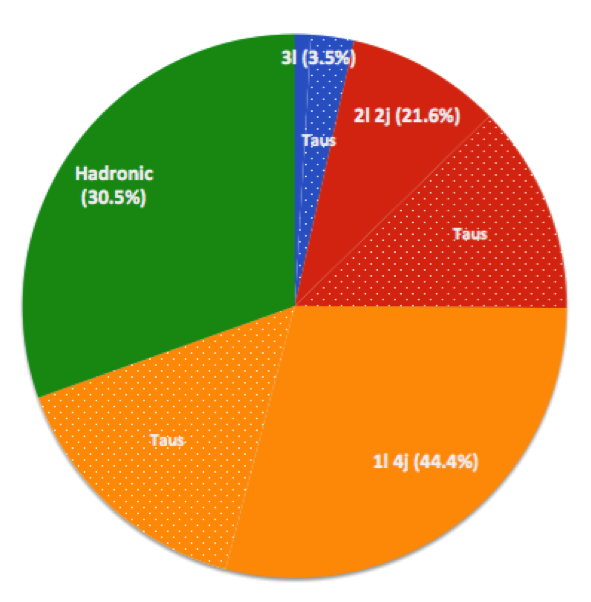
\includegraphics[scale=.8]{figures/branching_fractions.png}
\caption{Pie chart showing the different decay modes contributing 
to the total \xsec for the \www~process. 
The dotted areas indicate the portion of each decay 
mode which is due to the production of tau leptons.}
\label{fig:branching_fractions}
\end{figure}





\section{Data and Simulation Samples}
\subsection{Data}
\label{sec:subsection_data}



This analysis is based on the study of the full proton-proton collision
data from the LHC in 2012. After quality requirements, the amount 
of data used in this analysis corresponds to 
an integrated luminosity of \lumi.
The uncertainty on the integrated luminosity is $2.8\%$ 
following the same methodology as in \cite{Aad:2013ucp}.
%from Van-der-Meer scans taken throughout 2012.
%read this citation.
The data are selected after requiring that at least one
of a series of single lepton triggers passed during data taking, 
specifically, one of the following:
either an electron trigger 
requiring at least one isolated
electron with $\pt>24$~\GeV~, an electron trigger requiring
at least one (possibly non-isolated) electron 
with $\pt>60$~\GeV, a muon 
trigger requiring at least one isolated muon with $\pt>24$~GeV,
or a muon trigger requiring at least one 
(possibly non-isolated) muon with $\pt>36$~GeV.


\subsection{Simulation samples}
%%Do I need to talk about Monte Carlo showering, 
%%hadronization and reconstruction?
%%A general discussion of Monte Carlo could go here

An important tool for the modelling of physics processes
that are/could be produced at the LHC is Monte Carlo simulation (MC).
MC relies on random sampling to connect the matrix element formulations
derived from quantum mechanical pertubation theory into 
actual predictions for the results of proton-proton collisions
at the LHC.
The prediction of a single collision from the MC represents
one possible outcome of the proton-proton collision, with all of the 
products of the hard-scattering and their four-momenta.
This result can be passed through additional MC simulation to describe
hadronization and the soft products of the collision e.g. photon radiation.
Finally, these products are passed through a detailed 
simulation of the ATLAS detector built in \geant~\cite{Agostinelli:2002hh}
so that the same reconstruction algorithms
can be applied as in the data.
This sampling is repeated many times to populate the 
distribution of possible
outcomes. Dedicated MC programs are provided by theorists for 
different processes and to different orders in pertubation theory,
sometimes with different treatments.
Details of the different processes simulated from MC and their
treatment are presented below.




\subsubsection{Signal Processes}
\label{sec:signal}


%%%
%If I'm going to include this, I better read up on it.
%%%
%The production \xsec without Higgs contribution has been calculated 
%to $\mathcal{O}(\alpha_s)$  corrections in Ref~\cite{Binoth:2008kt}.
%$\mathcal{O}(\alpha_s)$ corrections, Higgs boson exchange and spin 
%correlations of $W$ bosons lepton decay are also available
%~\cite{Campanario:2008yg}.  

The SM $WWW$ signal processes are implemented in the Monte
Carlo generator \vbfnlo~\cite{Arnold:2011wj,Arnold:2012xn},
which can generate partonic events at leading-order (LO) in QCD with
next-to-leading-order (NLO) cross-sections, 
and in \madgraph~\cite{MadGraph}, which can generate
partonic events at NLO  with NLO cross-sections. 
The partonic events are further processed 
by \pythiaeight~\cite{Sjostrand:2007gs} and \photos~\cite{Golonka:2005pn} 
to add effects of beam remnant interactions and initial and 
final state radiation. 
SM parameters, such as the Higgs mass,
must be provided to the MC generators as input. 
The underlying event
parameters are set in \pythiaeight~ using the ATLAS tune 
of AU2\cite{atlas:2011zja}.
The MC generators must also be provided an appropriate PDF.
The PDF used  in the LO \vbfnlo~generation is
the LO CTEQ6L1~\cite{Pumplin:2002vw} PDF set;
CT10 NLO~\cite{guzzi:2011sv}
is used in the NLO \vbfnlo~cross-section calculation.
The PDF used in the NLO \madgraph~generation 
and \xsec~calculation is CTEQ6L1 
but this is re-weighted to CT10 NLO using a k-factor of 1.08 to 1.10.
Since the MC generators are computed to finite order in perturbation
theory, renormalization and factorization scales must be chosen.
The renormalization and factorization scales are dynamically
set to the $WWW$ invariant mass in the \vbfnlo~samples; they 
are set to a fixed scale equal to the $Z$ mass in \madgraph.
The \vbfnlo~samples are restricted to leptonic decays of the $W$~bosons
where each lepton has a \pt~of at least 5~\GeV. The \madgraph~
samples include all decays of the $W$~boson, with a requirement 
that jets have a a \pt~of at least 10~\GeV~ but with no requirement
on the \pt~of leptons.
They are compared in a common fiducial phase space,
described in more detail in \sec\ref{sec:fiducial}.
The \vbfnlo~ and \madgraph~samples handle interference 
between $WH\rightarrow WWW(*)$ 
and on-shell $WWW$ production at LO, but \madgraph~is not
able to do this at NLO. As a result, the NLO \madgraph~samples
are split into sepearate samples of 
on-shell \www~ and $WH\rightarrow WWW(*)$ production.
Both sets are further split by the \www~charge mode.
For each sample, the \xsecs are summarized in \tab\ref{tab:signal_xsec} 
in their full phase space and in the common fiducial phase space.
The fiducial \xsecs are observed to be nearly the same
between the two generators.
This serves as a good check of the understanding of the 
signal process. The \madgraph~\xsecs are used throughout the 
remainder of the analysis.

%Do I need to describe the k-factors?
%It would be nice to also add some distributions from Rivet comparing
%the two at truth level.


%Describe the pdf uncertainty calculation.
%what about renormalization and factorization scales




%\begin{table}[ht]
%\centering
%\begin{tabular}{|l||c|c||}
\hline
 & \vbfnlo & \madgraph \\
\hline
\hline
Higgs mass, $m_H$ & 126.0~\GeV & \\ 
Top mass, $m_t$ & 172.4~\GeV  & \\
$Z$ mass, $m_Z$ & 91.1876~\GeV & 91.188~\GeV\\
$W$ mass, $m_W$ & 80.398~\GeV & \\
Fermi constant, $G_F$ & $1.16637\times 10^{-5}~\GeV^{-2}$ & \\
\hline
\end{tabular} 


%\caption{List of the most relevant SM parameters used as input to the 
%signal MC generation.}
%\label{tab:signal_sm_parameters}
%\end{table}


\begin{table}[ht]
\centering
\begin{tabular}{|cc||c|c|c|}
\hline
\multicolumn{2}{|c||} {Sample} &  \multicolumn{2}{c|}{Cross-section [fb]} \\
                              && Inclusive & Fiducial \\
\hline
\hline
%\multirow{3}{*}{\vbfnlo~LO} & $W^{+}W^{+}W^{-}\rightarrow l\nu l\nu l\nu$ & $3.56 \pm 0.005$ & \\
%                            & $W^{-}W^{+}W^{-}\rightarrow l\nu l\nu l\nu$ & $1.88\pm0.003$ & \\ 
%			    \cline{2-4} 
%                            & Sum & $5.44\pm0.006$ & \\ 
%\hline
\multirow{3}{*}{\vbfnlo~NLO} & $W^{+}W^{+}W^{-}\rightarrow l\nu l\nu l\nu$ & $4.95 \pm 0.007$ & $0.2050 \pm 0.0070$\\
                           & $W^{-}W^{+}W^{-}\rightarrow l\nu l\nu l\nu$ & $2.65\pm0.004$ & $0.0987 \pm 0.0037$\\ 
			    \cline{2-4} 
                           %& $WWW\rightarrow l\nu l\nu l\nu$ & $7.60\pm0.008$ & \\ 
                           & Sum & $7.60\pm0.008$ & $0.3037 \pm 0.0072$\\ 
\hline
%With PDF KFactor
\multirow{5}{*}{\madgraph~NLO} & $W^{+}W^{-}W^{+}\rightarrow \textrm{Anything}$ &$59.47\pm0.11$ & $0.0900 \pm 0.0048$\\
                        & $W^{-}W^{+}W^{-} \rightarrow \textrm{Anything}$& $28.069\pm0.076$ & $0.0476 \pm 0.0043$\\
                        & $W^{+}H\rightarrow W^{+}W^{+}W^{-}(*)\rightarrow\textrm{Anything}$ & $99.106\pm0.019$ & $0.1114 \pm 0.0029$\\
                        & $W^{-}H\rightarrow W^{-}W^{+}W^{-}(*) \rightarrow \textrm{Anything}$& $54.804\pm0.010$ & $0.0603 \pm 0.0015$\\
			\cline{2-4} 
                        & Sum & $241.47\pm0.13$ & $0.3092 \pm 0.0072$\\
%Without PDF KFactor
%\multirow{5}{*}{\madgraph~NLO} & $W^{+}W^{-}W^{+}\rightarrow \textrm{Anything}$ &$55.07\pm0.10$ & $0.0818 \pm 0.0044$\\
%                        & $W^{-}W^{+}W^{-} \rightarrow \textrm{Anything}$& $25.99\pm0.07$ & $0.0433 \pm 0.0039$\\
%                        & $W^{+}H\rightarrow W^{+}W^{+}W^{-}(*)\rightarrow\textrm{Anything}$ & $91.765\pm0.018$ & $0.1013 \pm 0.0026$\\
%                        & $W^{-}H\rightarrow W^{-}W^{+}W^{-}(*) \rightarrow \textrm{Anything}$& $50.7440\pm0.0094$ & $0.0548 \pm 0.0014$\\
%			\cline{2-4} 
%                        & Sum & $223.57\pm0.12$ & $0.2812 \pm 0.0066$\\
\hline
\end{tabular}

\caption{Inclusive and common fiducial cross-sections at NLO 
for \vbfnlo~and \madgraph~samples. 
The sum of the inclusive \xsecs are different
because of the different branching fractions in the two cases. 
The sum of the fiducial cross-sections, however, are expected to be similar because
they are computed for the same phase space, as described in \sec\ref{sec:fiducial}.
Only statistical uncertainties are shown.}
\label{tab:signal_xsec}
\end{table}


%%%%
%soud I show the dependence on scales here?
%%%%
%The dependencies of the 
%$\xsecs on the choices of scales have been studied in the two
%references~\cite{Binoth:2008kt,Campanario:2008yg}. 

% The production at LO is a pure electroweak process. The
% NLO correction brings in $\alpha_s$ which actually makes the cross
% sections more sensitive to the choices of scales. 
%It has been pointed
%out that a jet veto should reduce the scale dependence. 

%The $W$ boson is short lived, so one must study its decay products.
%As already mentioned, the focus of this analysis is on the final state 


%need to also show the MadGraph parameters
%maybe rephrase so that I can discuss both in parallel
%get generation parameters from semi-leptonic note
%report both sets of cross-sections here
%include updated info on cross-sections and PDFs 

\begin{figure}[ht!]
\centering
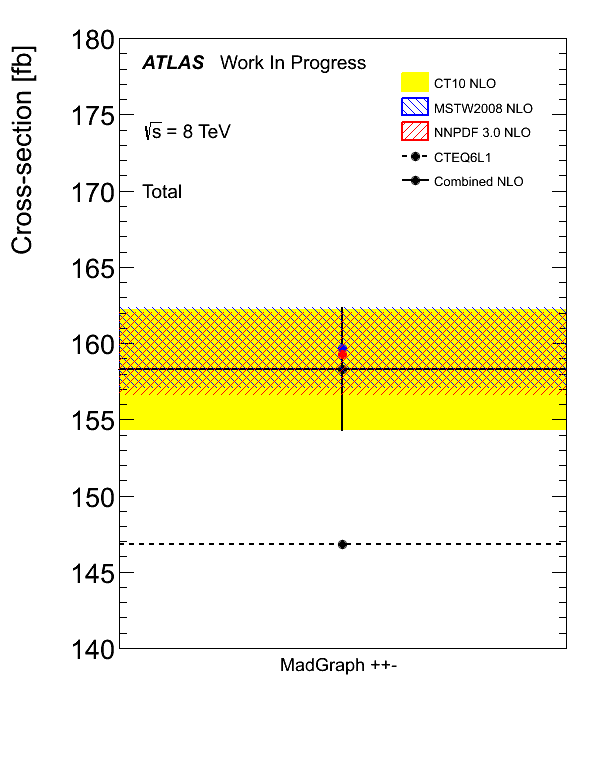
\includegraphics[width=.35\columnwidth]{figures/pdf/MADppm_total_cteq6l1.png}
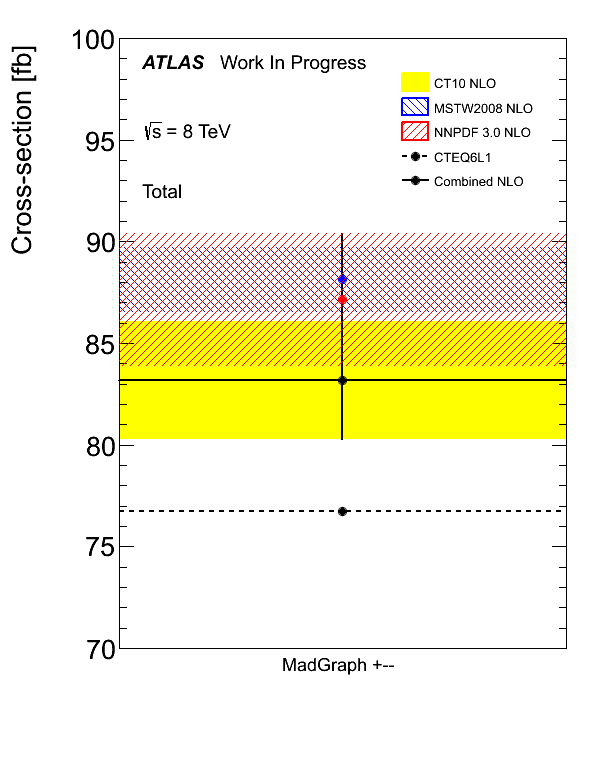
\includegraphics[width=.35\columnwidth]{figures/pdf/MADpmm_total_cteq6l1.png}
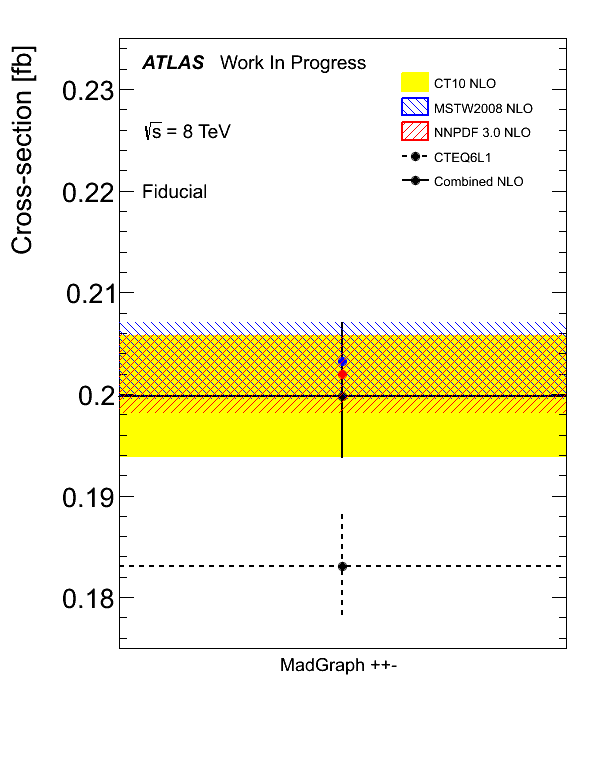
\includegraphics[width=.35\columnwidth]{figures/pdf/MADppm_fiducial_cteq6l1.png}
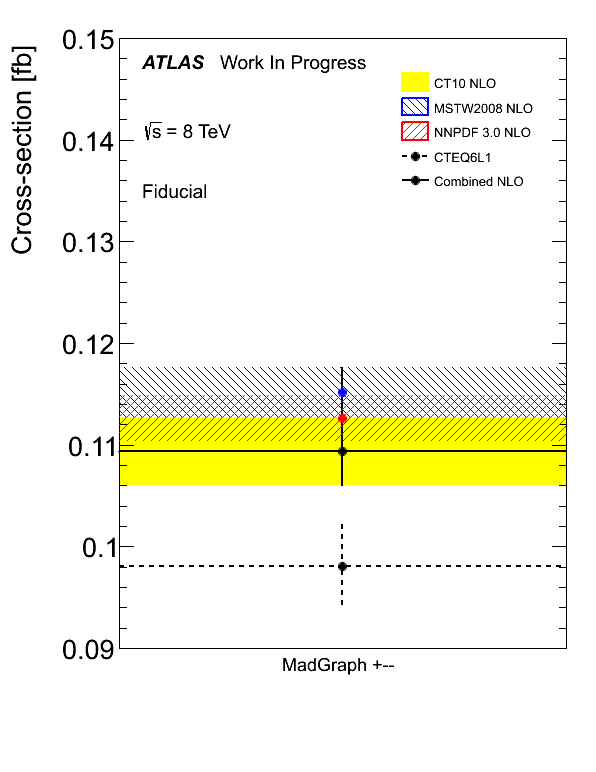
\includegraphics[width=.35\columnwidth]{figures/pdf/MADpmm_fiducial_cteq6l1.png}
\caption{The signal cross-sections for different PDFs along with their
uncertainties are shown on the {\sc MadGraph} $WWW$ signal samples
for the total $WWW$ phase space and branching fraction for
the $W^{+}W^{+}W^{-}$ (top left) and $W^{+}W^{-}W^{-}$ (top right)
charge modes
and in the fiducial region for $W^{+}W^{+}W^{-}$ (bottom left) 
and $W^{+}W^{-}W^{-}$ (bottom right).
The bands show the PDF uncertainty for CT10 NLO (solid yellow),
MSTW 2008 NLO (hashed blue), and NNPDF 3.0 NLO (hashed red). The
solid line shows the envelope of all uncertainty bands used as the final
PDF uncertainty estimate. The central value of CT10 NLO is taken as the
central value of the estimate.
The dashed-line shows the cross-section and 
statistical uncertainty for the CTEQ6L1
pdf sets used in the original generation step.}
\label{fig:signal_pdf_unc}
\end{figure}

\begin{table}[ht!]
\centering
\begin{tabular}{c|c|c}
\hline
 & \multicolumn{2}{c}{PDF Uncertainty}\\
 & $W^{+}W^{+}W^{-}$ & $W^{+}W^{-}W^{-}$ \\
\hline
\hline
Total & $+2.58\%~-2.51\%$ &  $+8.69\%~-3.47\%$ \\
Fiducial & $+3.64\%~-3.00\%$ & $+7.57\%~-3.08\%$ \\
\hline
\end{tabular}
\caption{Summary of PDF uncertainties estimated on NLO {\sc MadGraph} cross-sections
in both the fiducial and total phase space.}
\label{tab:pdfunc}
\end{table}

Uncertainties on the signal prediction mainly come from the choice of PDF, 
the inherent PDF uncertainty, and the renormalization and factorization
scales, as described in \sec\ref{sec:pdf}.
The uncertainty due to the choice of PDF is derived for the {\sc MadGraph} 
cross-sections following a modified version of the pdf4lhc
\cite{Botje:2011sn} recommendations.  The resulting 
uncertainty is shown separately for the two different charge modes
in both the fiducial and the inclusive phase
space in Table~\ref{tab:pdfunc}.
The uncertainty is determined by comparing three different PDFs:
CT10 NLO~\cite{Lai:2010vv}, MSTW2008 NLO~\cite{Martin:2009iq}, 
and NNPDF 3.0 NLO~\cite{Ball:2014uwa}. 
This comparison is presented in \fig\ref{fig:signal_pdf_unc}.  
Symmetric 68\% CL uncertainties 
are determined for CT10 NLO and MSTW 2008 NLO using the 68\% CL 
set provided for MSTW directly and the 90\%CL set for CT10 after
scaling down by 
a factor of 1.645 in order to approximate a 68 \% CL uncertainty. 
The uncertainty of the NNPDF 3.0 NLO PDF set is 
determined by using the standard deviation of the distribution 
of 101 MC PDFs provided in the PDF set; the nominal value is taken
from the mean of the same PDFs.  
The CT10 NLO PDF central value is used as the nominal 
value of the final estimate.
The final PDF uncertainty on that estimate is
taken as the envelope of the uncertainty bands for all three PDF sets.  



The uncertainty on the factorization and renormalization scales are 
determined by varying each of them independently up or down by 
a factor of two. 
The effect of these variations on the cross-sections
as compared to the nominal
are shown separately for the two different charge 
modes in \tab~\ref{tab:scaleVariation}.
The symmetric uncertainty is then determined by taking the maximum 
variation for each charge mode, 
namely, 2.62\% for $W^+W^+W^-$ and 2.53\% for $W^-W^+W^-$. 

\begin{table}[ht!]
    \centering
\begin{tabular}{cc|ccc}
\hline
& \backslashbox{$\mu_F$}{$\mu_R$}     & $\frac{1}{2}M_{WWW}$ & $M_{WWW}$ &  $2M_{WWW}$ \\
\cline{2-5}
\multirow{3}{*}{\Wp\Wp\Wm} &$\frac{1}{2}M_{WWW}$ & 2.62\% & -0.14\% & -2.11\% \\
%\cline{2-5}
&$M_{WWW}$ & 2.13\% & 0 & -2.41\% \\
%\cline{2-5}
&$2M_{WWW}$ & 1.56\% & 0.24\% & -2.42\% \\
\hline
\hline
& \backslashbox{$\mu_F$}{$\mu_R$}     & $\frac{1}{2}M_{WWW}$ & $M_{WWW}$ &  $2M_{WWW}$ \\
\cline{2-5}
\multirow{3}{*}{\Wm\Wp\Wm} &$\frac{1}{2}M_{WWW}$ & 1.91\% & 1.38\% & -2.00\% \\
%\cline{2-5}
&$M_{WWW}$ & 1.61\% & 0 & -2.53\% \\
%\cline{2-5}
&$2M_{WWW}$ & 1.25\% & -1.05\% & -2.12\% \\
\hline
\end{tabular}
\caption{The relative variation of the NLO cross sections corresponding 
to different choices of factorization and renormalization 
scales for the \Wp\Wp\Wm and \Wm\Wp\Wm  processes. }
\label{tab:scaleVariation}
\end{table}

The signal cross-sections and uncertainties are thus determined to be 
\begin{equation}
\sigma^{\textrm{Total}}_{\textrm{Theory}}= 241.47\pm0.13 ~(\textrm{Stat.}) ~^{+10.33}_{-6.08} ~(\textrm{PDF}) ~\pm 6.3 ~(\textrm{Scale}) ~\textrm{fb} %uncertainty?
\end{equation}
for the inclusive \xsec and
\begin{equation}
\label{eq:fiducial_theory}
\sigma^{\textrm{Fiducial}}_{\textrm{Theory}}= 309.2\pm7.2 ~(\textrm{Stat.}) ~^{+15.05}_{-8.36} ~(\textrm{PDF}) ~\pm 8.0 ~(\textrm{Scale}) ~\textrm{ab} %uncertainty?
\end{equation}
for the fiducial cross-section.


%should i include this
%The analysis considers events with three leptons ($e$ or $\mu$) in the final state. The contributions from events in which $W$ bosons decay to $\tau$'s, and the $\tau$'s sequentially decay to $e$ or $\mu$ should be included and is expected to be 40\% of total yield of the 3-lepton final state.  


\subsubsection{aQGC signal}
\label{sec:aqgc_signal}

MC samples of the aQGC signal processes described in \sec\ref{sec:eft}
have been generated using \vbfnlo at NLO in QCD.  (but don't we use LO?)
The cross-sections for the aQGC signal depend on the values
of the couplings $f_{s,0}$ and $f_{s,1}$. MC samples have 
been generated for a grid of points in the $f_{s,0}$ vs $f_{s,1}$ space
and their cross-sections are shown in \fig\ref{fig:aqgc_total_xsec_ununitarized_3l}. %histogram of cross-sections

\begin{figure}[ht!]
\centering
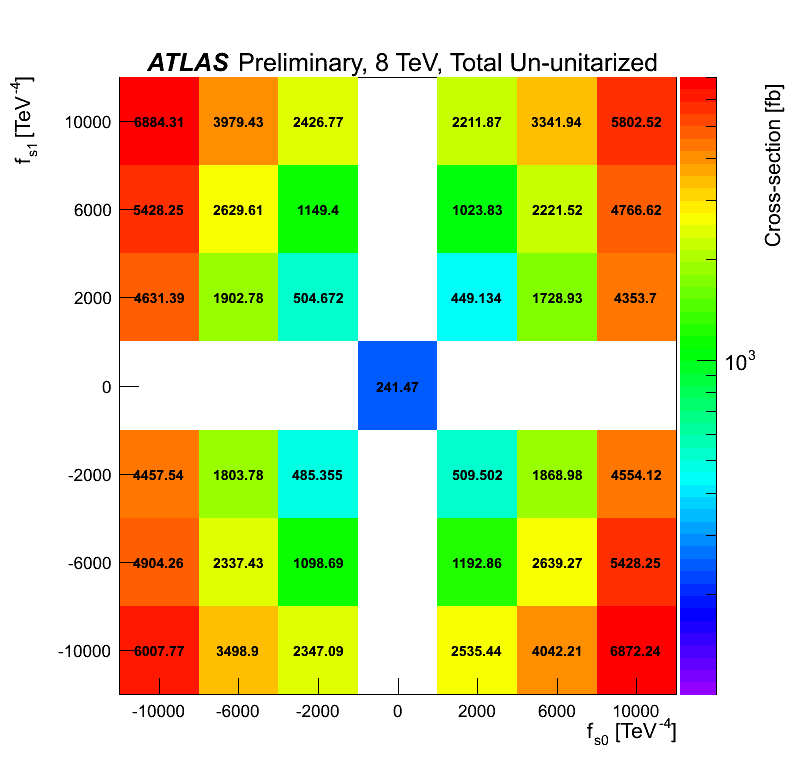
\includegraphics[width=.8\textwidth]{figures/aQGC/total_xsec/www_3l_aqgc_total_ununitarized_noratio.png}
\caption{Total cross-section for non-unitarized aQGC signal samples as a function of $f_{s,0}$ vs $f_{s,1}$.
The total SM cross-section is shown at $f_{s,0}=f_{s,1}=0$ for comparison.}
\label{fig:aqgc_total_xsec_ununitarized_3l}
\end{figure}

The issues of unitarity violation \sec\ref{sec:eft} are taken
into account using a form factor like in \eqn\eqref{eq:form_factor}.
The choices of the exponent, $n$, and form factor scale, $\Lambda$, 
are somewhat ad-hoc. Furthermore, a complete study of the unitarity
behavior of this process has never been performed, so there are not
currently detailed prescriptions on what to choose. 
However, based on discussions with the authors of \vbfnlo, who
are at the moment trying to perform these studies, an exponent
of $n=1$ is expected to be sufficient to achieve unitarity 
for this process.  As for the choice of $\Lambda$, we have
chosen to look at a few different values, which cover a wide
range but which should follow a smooth interpolation. 
This has the advantage of providing information about the
sensitivity to the form factor that can be interpreted 
by theorists as they see fit. Dedicated MC samples
are generated with the unitarization applied for values
of $\Lambda =$ 500~\GeV, 1000~\GeV, 2000~\GeV, and 3000~\GeV.
The cross-sections for each of these unitarization cases
are shown in \fig\ref{fig:aqgc_total_xsec_unitarized_3l}.

\begin{figure}[ht!]
\centering
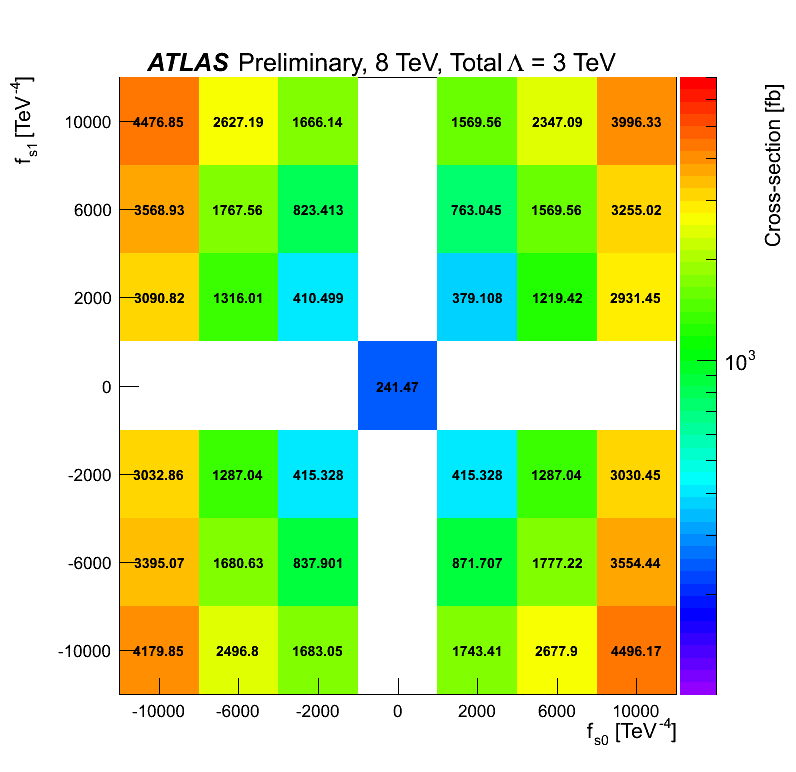
\includegraphics[width=.45\textwidth]{figures/aQGC/total_xsec/www_3l_aqgc_total_3TeV_noratio.png}
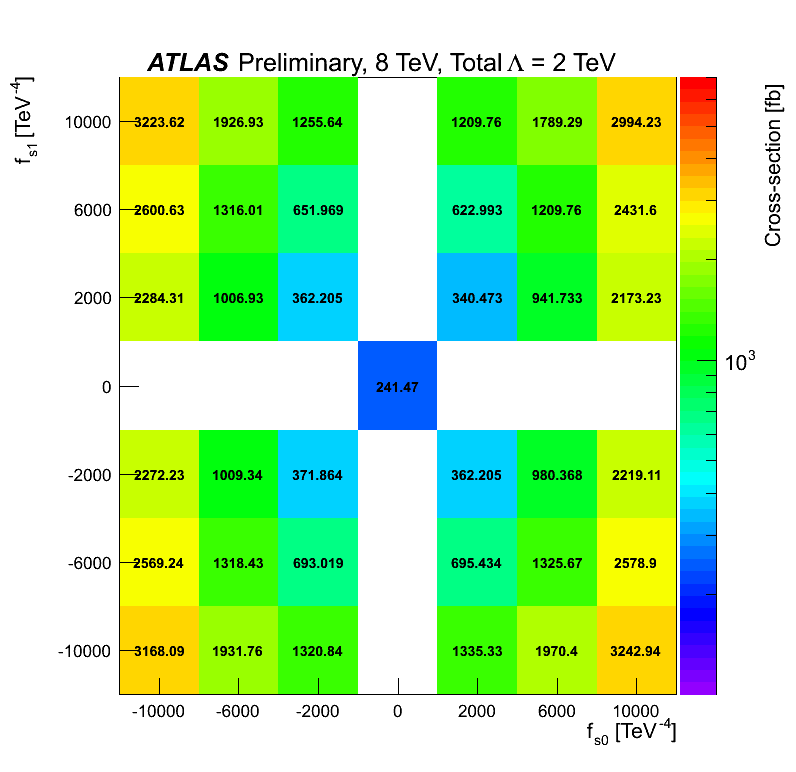
\includegraphics[width=.45\textwidth]{figures/aQGC/total_xsec/www_3l_aqgc_total_2TeV_noratio.png}
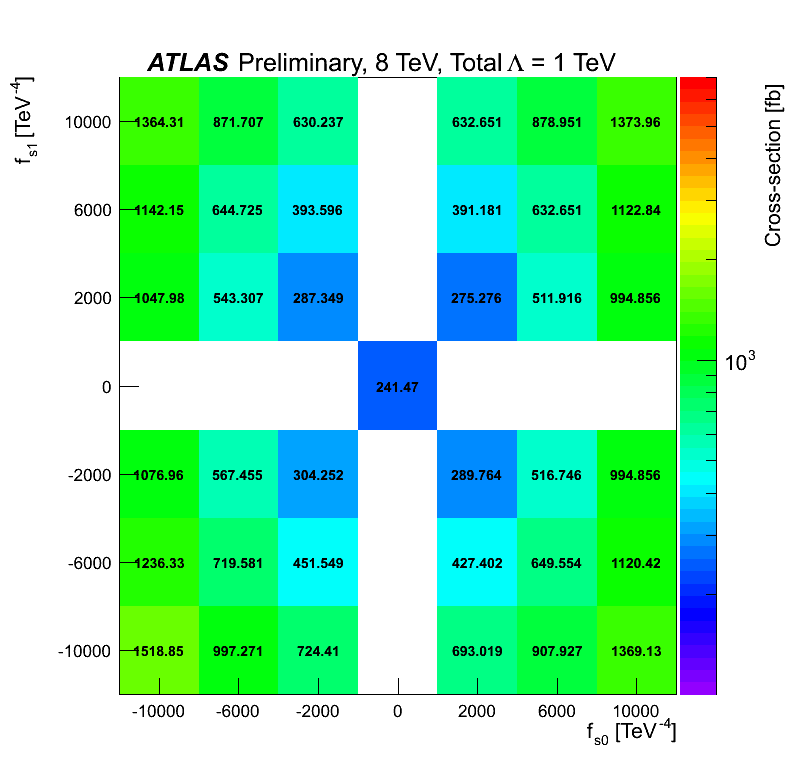
\includegraphics[width=.45\textwidth]{figures/aQGC/total_xsec/www_3l_aqgc_total_1TeV_noratio.png}
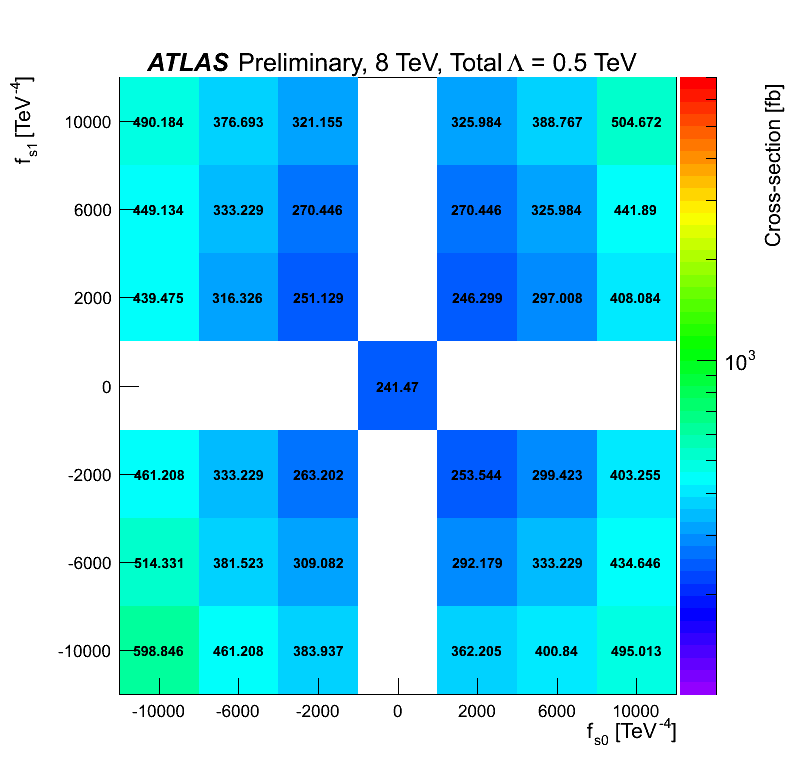
\includegraphics[width=.45\textwidth]{figures/aQGC/total_xsec/www_3l_aqgc_total_p5TeV_noratio.png}
\caption{Total cross-section for unitarized aQGC signal samples as a function of $f_{s,0}$ vs $f_{s,1}$.
Four different values of the unitarization scale, $\Lambda$, are chosen: 3~\TeV~(Top Left),
2~\TeV~(Top Right), 1~\TeV~(Bottom Left), and 0.5~\TeV~(Bottom Right).
The total SM cross-section is shown at $f_{s,0}=f_{s,1}=0$ for comparison.}
\label{fig:aqgc_total_xsec_unitarized_3l}
\end{figure}
























\newpage

\subsubsection{Backgrounds samples}
\label{sec:subsection_datasets_MC}

Only processes containing 3 or more prompt
leptons ($WZ$, $ZZ$, $t\bar{t}V$, $VVV$), or 2 leptons and an 
isolated photon ($Z+\gamma$) are estimated using MC simulation 
samples in this analysis. The other processes are estimated from 
data as this will be explained in Section~\ref{sec:backgrounds_estimation}. 
The samples listed in this section and containing less than 3 prompt leptons 
have been used for preliminary or dedicated studies, but are not used for 
the determination of the final results. The MC samples are pass through the 
GEANT4~\cite{Agostinelli:2002hh} simulation~\cite{Aad:2010ah} of the ATLAS 
detector and reconstructed in the same way as the data.

The diboson and triboson samples are listed in Table~\ref{tab:sample_bkg_dibosons}. The triboson samples other than the signal, \textit{ie}: $ZWW^{*}$ and $ZZZ^{*}$ were generated using the MadGraph~\cite{Alwall_madgraph} generator, hadronized through the Pythia6~\cite{PYTHIA} parton shower, with the AUET2B~\cite{ATL-PHYS-PUB-2011-009} tunes and the CTEQ6L1~\cite{Pumplin:2002vw} PDF set. The $Z\gamma$ samples were generated with the Sherpa~\cite{sherpa} generator and the CT10~\cite{Guzzi:2011sv} PDF set. The $W\gamma$ samples were generated with the AlpGen~\cite{ALPGEN} generator, hadronized through JIMMY~\cite{Jimmy}, with the AUET2C~\cite{ATL-PHYS-PUB-2011-009} tunes and the CTEQ6L1 PDF set. Other diboson samples ($WW$, $WZ$, $ZZ$) were obtained using the Powheg~\cite{Alioli:2008gx,Nason:2004rx,Frixione:2007vw,Alioli:2010xd} generator, hadronized through the Pythia8~\cite{Sjostrand:2007gs} parton shower, with the AU2~\cite{atlasmctunes} tunes and the CT10 PDF set. Dedicated high-stat $WZ$ and $ZZ$ samples were generated to increase the statistics in all the signal region used in this analysis. They were obtained requesting the presence of 3 leptons with $\pt>7~\GeV$.

The dibosons samples where the production is due to loop induced process or Double Parton Scattering (DPS) processes are summarized in Table~\ref{tab:sample_bkg_dibosons_gg2DPI}. The loop induced processes were generated using the gg2ZZ~\cite{Binoth:2008pr} and gg2WW~\cite{Binoth:2006mf} generators, hadronized using JIMMY, with the AU2 tunes and the CT10 PDF set. The DPS processes were generated with the AU2 tunes and the CTEQ6L1 PDF set. The cross section of these processes have been evaluated for the ATLAS same sign WW analysis~\cite{Aad:2014zda}, as this will be explained in Section~\ref{sec:bkg_DPS}.

Single boson processes are summarized in Table~\ref{tab:sample_bkg_Zjets} for the $Z+$jets samples and in Table~\ref{tab:sample_bkg_wjets} for the $W+$jets samples. The $Z+$jets samples were generated with the Sherpa generator and the CT10 PDF set. Low mass Drell-Yan samples were not simluated using the GEANT4 simulation, but with the AF2 simulation, however dedicated scale factors are applied for these samples, when they are used, in the analysis. The $W+$jets samples were generated with the AlpGen generator, hadronized through JIMMY, with the AUET2C tunes and the CTEQ6L1 PDF set.

Samples containing top quarks are summarized in Table~\ref{tab:sample_bkg_top}. $t\bar{t}$ events were generated using the MCatNLO\cite{MCatNLO} generator, hadronized through JIMMY with the CT10 PDF set. Single top samples in the s-channel and in the $Wt$ channel were generated using MCatNLO hadronized through JIMMY with the CT10 PDF set. Single top samples in the t-channel were generated using AcerMC\cite{Kersevan:2004yg}, hadronized using PYTHIA6 with the AUET2B tunes and the CTEQ6L1 PDF set. Finally $t\bar{t}V$ processes were generated using the MadGraph generator, hadronized through the Pythia6 parton shower, with the AUET2B tunes and the CTEQ6L1PDF set.


 % the $Z+jets$ samples in Table~\ref{tab:sample_bkg_Zjets}, the $W+jets$ in Table~\ref{tab:sample_bkg_wjets}, and samples containing top quarks in Table~\ref{tab:sample_bkg_top}.

When $Z+$jets and $Z+\gamma$ samples are used simultaneously, an overlap removal procedure must be used to avoid double counting of FSR events. Events containing an FSR photon with $E_{T}>10~\GeV$ are explicitely vetoed out from the $Z+$jets sample. The algorithm used is the same as what was developped in the $8~\TeV$ ATLAS $WZ$ analysis~\cite{Anger:1663539}.


\begin{table}[ht!]
  \centering
  \begin{footnotesize}
\begin{tabular}{c|c|c|c|c|c|c}
\hline
    &  &  & Cross-Section &  & Event filter  \\
  Sample  & Generator & Sample type & [pb] & k-factor &  efficiency  & used in signal region\\
\hline \hline
167007 & MadGraphPythia & ZWWStar lllnulnu  &  0.0015546  &  1  &  1 & Yes \\
167008 & MadGraphPythia & ZZZStar nunullll  &  0.00033239  &  1  &  1 & Yes \\
145161 & Sherpa & eegammaPt10  &  32.26  &  1  &  1 & Yes \\
145162 & Sherpa & mumugammaPt10  &  32.317  &  1  &  1 & Yes \\
%146430 & AlpgenJimmy & Wgamma Np0 & 230.09 & 1.15 & 1 & No \\
%146431 & AlpgenJimmy & Wgamma Np1 & 59.343 & 1.15 & 1 & No \\
%146432 & AlpgenJimmy & Wgamma Np2 & 21.469 & 1.15 & 1 & No \\
%146433 & AlpgenJimmy & Wgamma Np3 & 7.1032 & 1.15 & 1 & No \\
%146434 & AlpgenJimmy & Wgamma Np4 & 2.1224 & 1.15 & 1 & No \\
%146435 & AlpgenJimmy & Wgamma Np5 & 0.46612 & 1.15 & 1 & No \\
146436 & AlpgenJimmy & Wgamma Np0 & 229.88 & 1.15 & 0.31372 & No \\
146437 & AlpgenJimmy & Wgamma Np1 & 59.518 & 1.15 & 0.44871 & No \\
146438 & AlpgenJimmy & Wgamma Np2 & 21.39  & 1.15 & 0.54461 & No \\
146439 & AlpgenJimmy & Wgamma Np3 & 7.1203 & 1.15 & 0.62974 & No \\
126928 & PowhegPythia8& WpWm ee  &  0.62  &  1.0  &  1 & No  \\
126929 & PowhegPythia8& WpWm me  &  0.62  &  1.0  &  1 & No  \\
126930 & PowhegPythia8& WpWm te  &  0.62  &  1.0  &  1 & No  \\
126931 & PowhegPythia8& WpWm em  &  0.62  &  1.0  &  1 & No \\
126932 & PowhegPythia8& WpWm mm  &  0.62  &  1.0  &  1 & No \\
126933 & PowhegPythia8& WpWm tm  &  0.62  &  1.0  &  1 & No \\
126934 & PowhegPythia8& WpWm et  &  0.62  &  1.0  &  1 & No \\
126935 & PowhegPythia8& WpWm mt  &  0.62  &  1.0  &  1 & No \\
126936 & PowhegPythia8& WpWm tt  &  0.62  &  1.0  &  1 & No \\

185813 & PowhegPythia8& ZZ 4e mll4 TriLeptonFilter & 0.07677 & 1 & 0.57204 & Yes \\
185814 & PowhegPythia8& ZZ 2e2mu mll4 TriLeptonFilter & 0.1757 & 1 & 0.49893 & Yes \\
185815 & PowhegPythia8& ZZ 2e2tau mll4 TriLeptonFilter & 0.1757 & 1 & 0.086032 & Yes \\
185816 & PowhegPythia8& ZZ 4mu mll4 TriLeptonFilter & 0.07677 & 1 & 0.58293 & Yes \\
185817 & PowhegPythia8& ZZ 2mu2tau mll4 TriLeptonFilter & 0.1757 & 1 & 0.087166 & Yes \\
185818 & PowhegPythia8& ZZ 4tau mll4 TriLeptonFilter & 0.07677 & 1 & 0.0076557 & Yes \\

181471 & Sherpa & $ZZ*\rightarrow eeee$  $m_{Z,1} > 4$~GeV, $m_{Z,2} < 4$~GeV  & 2.8286 & 0.880 & 1.0 & No \\
181472 & Sherpa & $ZZ*\rightarrow ee\mu\mu$ $m_{Z,1} > 4$~GeV, $m_{Z,2} < 4$~GeV  & 2.34503 & 0.880 & 1.0 & No \\
181473 & Sherpa & $ZZ*\rightarrow ee\tau\tau$ $m_{Z,1} > 4$~GeV, $m_{Z,2} < 4$~GeV  & 1.59326 & 0.880 & 1.0 & No \\
181474 & Sherpa & $ZZ*\rightarrow \mu\mu ee$ $m_{Z,1} > 4$~GeV, $m_{Z,2} < 4$~GeV  & 0.48613 & 0.880 & 1.0 & No \\
181475 & Sherpa & $ZZ*\rightarrow \mu\mu\mu\mu$ $m_{Z,1} > 4$~GeV, $m_{Z,2} < 4$~GeV  & 0.50835 & 0.880 & 1.0 & No \\
181476 & Sherpa & $ZZ*\rightarrow \mu\mu\tau\tau$ $m_{Z,1} > 4$~GeV, $m_{Z,2} < 4$~GeV  & 0.42288 & 0.880 & 1.0 & No \\
181477 & Sherpa & $ZZ*\rightarrow \tau\tau ee$ $m_{Z,1} > 4$~GeV, $m_{Z,2} < 4$~GeV  & 0.00403 & 0.880 & 1.0 & No \\
181478 & Sherpa & $ZZ*\rightarrow \tau\tau\mu\mu$ $m_{Z,1} > 4$~GeV, $m_{Z,2} < 4$~GeV  & 0.00401 & 0.880 & 1.0 & No \\
181479 & Sherpa & $ZZ*\rightarrow \tau\tau\tau\tau$ $m_{Z,1} > 4$~GeV, $m_{Z,2} < 4$~GeV  & 0.00411 & 0.880 & 1.0 & No \\


% 126937 & PowhegPythia8& ZZ 4e mll4 2pt5  &  0.0735  &  1.0  &  0.90765 \\
% 126938 & PowhegPythia8& ZZ 2e2mu mll4 2pt5  &  0.1708  &  1.0  &  0.82724 \\
% 126939 & PowhegPythia8& ZZ 2e2tau mll4 2pt5  &  0.1708  &  1.0  &  0.58278 \\
% 126940 & PowhegPythia8& ZZ 4mu mll4 2pt5  &  0.0735  &  1.0  &  0.91241 \\
% 126941 & PowhegPythia8& ZZ 2mu2tau mll4 2pt5  &  0.1708  &  1.0  &  0.58725 \\
% 126942 & PowhegPythia8& ZZ 4tau mll4 2pt5  &  0.0735  &  1.0  &  0.10604 \\
126949 & PowhegPythia8& ZZllnunu ee mll4  &  0.168  &  1  &  1 & No \\
126950 & PowhegPythia8& ZZllnunu mm mll4  &  0.168  &  1  &  1 & No \\
126951 & PowhegPythia8& ZZllnunu tt mll4  &  0.168  &  1  &  1 & No \\
185795  &  PowhegPythia8 &  WmZ 3e mll0p25 TriLeptonFilter  &  0.9655  &  1  &  0.051928 & Yes \\
185796  &  PowhegPythia8 &  WmZ e2mu mll0p4614 TriLeptonFilter  &  0.6326  &  1  &  0.073874  & Yes \\
185797  &  PowhegPythia8 &  WmZ e2tau mll3p804 TriLeptonFilter  &  0.1125  &  1  &  0.012544  & Yes \\
185798  &  PowhegPythia8 &  WmZ mu2e mll0p25 TriLeptonFilter  &  0.9687  &  1  &  0.054302  & Yes \\
185799  &  PowhegPythia8 &  WmZ 3mu mll0p4614 TriLeptonFilter  &  0.6479  &  1  &  0.071268  & Yes \\
185800  &  PowhegPythia8 &  WmZ mu2tau mll3p804 TriLeptonFilter  &  0.1125  &  1  &  0.01258  & Yes \\
185801  &  PowhegPythia8 &  WmZ tau2e mll0p25 TriLeptonFilter  &  0.9687  &  1  &  0.012075  & Yes \\
185802  &  PowhegPythia8 &  WmZ tau2mu mll0p4614 TriLeptonFilter  &  0.6326  &  1  &  0.01664 & Yes \\
185803  &  PowhegPythia8 &  WmZ 3tau mll3p804 TriLeptonFilter  &  0.1108  &  1  &  0.0034037  & Yes \\
185804  &  PowhegPythia8 &  WpZ 3e mll0p25 TriLeptonFilter  &  1.416  &  1  &  0.053051 & Yes  \\
185805  &  PowhegPythia8 &  WpZ e2mu mll0p4614 TriLeptonFilter  &  0.9421  &  1  &  0.075904  & Yes \\
185806  &  PowhegPythia8 &  WpZ e2tau mll3p804 TriLeptonFilter  &  0.1755  &  1  &  0.013867 & Yes  \\
185807  &  PowhegPythia8 &  WpZ mu2e mll0p25 TriLeptonFilter  &  1.412  &  1  &  0.055296 & Yes  \\
185808  &  PowhegPythia8 &  WpZ 3mu mll0p4614 TriLeptonFilter  &  0.9572  &  1  &  0.073362 & Yes  \\
185809  &  PowhegPythia8 &  WpZ mu2tau mll3p804 TriLeptonFilter  &  0.1755  &  1  &  0.013891 & Yes \\
185810  &  PowhegPythia8 &  WpZ tau2e mll0p25 TriLeptonFilter  &  1.412  &  1  &  0.012105 & Yes  \\
185811  &  PowhegPythia8 &  WpZ tau2mu mll0p4614 TriLeptonFilter  &  0.9421  &  1  &  0.016718 & Yes  \\
185812  &  PowhegPythia8 &  WpZ 3tau mll3p804 TriLeptonFilter  &  0.172  &  1  &  0.0036427 & Yes  \\
% 129477 & PowhegPythia8& WZ Wm11Z11 mll0p250d0 2LeptonFilter5  &  1.407  &  1.0  &  0.29456 \\
% 129478 & PowhegPythia8& WZ Wm11Z13 mll0p4614d0 2LeptonFilter5  &  0.9382  &  1.0  &  0.35211 \\
% 129479 & PowhegPythia8& WZ Wm11Z15 mll3p804d0 2LeptonFilter5  &  0.1746  &  1.0  &  0.16682 \\
% 129480 & PowhegPythia8& WZ Wm13Z11 mll0p250d0 2LeptonFilter5  &  1.399  &  1.0  &  0.29351 \\
% 129481 & PowhegPythia8& WZ Wm13Z13 mll0p4614d0 2LeptonFilter5  &  0.9537  &  1.0  &  0.35132 \\
% 129482 & PowhegPythia8& WZ Wm13Z15 mll3p804d0 2LeptonFilter5  &  0.1746  &  1.0  &  0.16863 \\
% 129483 & PowhegPythia8& WZ Wm15Z11 mll0p250d0 2LeptonFilter5  &  1.399  &  1.0  &  0.14289 \\
% 129484 & PowhegPythia8& WZ Wm15Z13 mll0p4614d0 2LeptonFilter5  &  0.9382  &  1.0  &  0.18256 \\
% 129485 & PowhegPythia8& WZ Wm15Z15 mll3p804d0 2LeptonFilter5  &  0.1719  &  1.0  &  0.058517 \\
% 129486 & PowhegPythia8& WZ W11Z11 mll0p250d0 2LeptonFilter5  &  0.9795  &  1.0  &  0.29694 \\
% 129487 & PowhegPythia8& WZ W11Z13 mll0p4614d0 2LeptonFilter5  &  0.639  &  1.0  &  0.35302 \\
% 129488 & PowhegPythia8& WZ W11Z15 mll3p804d0 2LeptonFilter5  &  0.1125  &  1.0  &  0.15969 \\
% 129489 & PowhegPythia8& WZ W13Z11 mll0p250d0 2LeptonFilter5  &  0.9359  &  1.0  &  0.29766 \\
% 129490 & PowhegPythia8& WZ W13Z13 mll0p4614d0 2LeptonFilter5  &  0.6488  &  1.0  &  0.35414 \\
% 129491 & PowhegPythia8& WZ W13Z15 mll3p804d0 2LeptonFilter5  &  0.1125  &  1.0  &  0.16023 \\
% 129492 & PowhegPythia8& WZ W15Z11 mll0p250d0 2LeptonFilter5  &  0.9359  &  1.0  &  0.14803 \\
% 129493 & PowhegPythia8& WZ W15Z13 mll0p4614d0 2LeptonFilter5  &  0.639  &  1.0  &  0.18657 \\
% 129494 & PowhegPythia8& WZ W15Z15 mll3p804d0 2LeptonFilter5  &  0.1107  &  1.0  &  0.056651 \\
\hline 
\end{tabular}
\end{footnotesize}
\caption{List of diboson samples used in the analysis. 
For the three lepton signal regions, it is indicated for each
sample whether or not the sample is used.  If not, it is replaced
by a data-driven fake estimate described in Section~\ref{sec:fakebg}.
All samples are used in dilepton control regions.
}
\label{tab:sample_bkg_dibosons}
\end{table}


\begin{table}[ht!]
  \centering
  \begin{footnotesize}
\begin{tabular}{c|c|c|c|c|c|c}
\hline
    &  &  & Cross-Section &  & Event filter  \\
  Sample  & Generator & Sample type & [pb] & k-factor &  efficiency  & used in signal region\\
\hline \hline
116600 & gg2ZZJimmy & ZZ4lep & 0.00459 & 1 & 1 & Yes \\
116601 & gg2ZZJimmy & ZZ4e & 0.000675 & 1 & 1  & Yes \\
116602 & gg2ZZJimmy & ZZ4mu & 0.000675 & 1 & 1  & Yes \\
116603 & gg2ZZJimmy & ZZ2e2mu & 0.00134539 & 1 & 1 & Yes  \\
169471 & gg2wwJimmy & WpWmenuenu & 0.017 & 1 & 1   & No \\
169472 & gg2wwJimmy & WpWmenumunu & 0.017 & 1 & 1  & No  \\
169473 & gg2wwJimmy & WpWmenutaunu & 0.017 & 1 & 1 & No  \\
169474 & gg2wwJimmy & WpWmmunumunu & 0.017 & 1 & 1 & No   \\
169475 & gg2wwJimmy & WpWmmunuenu & 0.017 & 1 & 1  & No  \\
169476 & gg2wwJimmy & WpWmmunutaunu & 0.017 & 1 & 1  & No  \\
169477 & gg2wwJimmy & WpWmtaunutaunu & 0.017 & 1 & 1 & No   \\
169478 & gg2wwJimmy & WpWmtaunuenu & 0.017 & 1 & 1   & No \\
169479 & gg2wwJimmy & WpWmtaunumunu & 0.017 & 1 & 1  & No  \\
147280 & Pythia8 & DPI W W 2l & 0.0258 & 1 & 0.48 & Yes  \\
147281 & Pythia8 & DPI W W 2l2j & 0.0258 & 1 & 0.0752 & Yes  \\
147282 & Pythia8 & DPI W Z 2l & 0.139 & 1 & 0.0539 & Yes  \\
147283 & Pythia8 & DPI W Z 2l2j & 0.139 & 1 & 0.00873 & Yes  \\
147284 & Pythia8 & DPI W gamma 1l1gm & 9.86 & 1 & 0.159 & Yes  \\
147285 & Pythia8 & DPI Z Z 2l & 0.213 & 1 & 0.0547 & Yes  \\
147286 & Pythia8 & DPI Z Z 2l2j & 0.213 & 1 & 0.00457 & Yes  \\
147287 & Pythia8 & DPI Z gamma 1l1gm & 26.5 & 1 & 0.012 & Yes  \\
147288 & Pythia8 & DPI WZ dijet 2l2j & 1.43 & 1 & 0.102 & Yes  \\
147289 & Pythia8 & DPI ZZ dijet 2l2j & 1.86 & 1 & 0.0422 & Yes  \\
147290 & Pythia8 & DPI W diphoton 1l2gm & 0.012 & 1 & 0.0632 & Yes  \\
147291 & Pythia8 & DPI Zll diphoton 1l2gm & 0.00581 & 1 & 0.0259 & Yes  \\
147292 & Pythia8 & DPI Zvv diphoton 2gm & 0.00221 & 1 & 0.0898 & Yes  \\
147293 & Pythia8 & DPI gamma gamma 2gm & 943 & 1 & 0.00422 & Yes  \\
\hline 
\end{tabular}
\end{footnotesize}
\caption{List of loop induced, or DPI, diboson samples used in the analysis.
For the three lepton signal regions, it is indicated for each
sample whether or not the sample is used.  If not, it is replaced
by a data-driven fake estimate described in Section~\ref{sec:fakebg}.
All samples are used in dilepton control regions.
}
\label{tab:sample_bkg_dibosons_gg2DPI}
\end{table}




\begin{table}[ht!]
  \centering
  \begin{footnotesize}
  
\begin{tabular}{c|c|c|c|c|c|c}
\hline
    &  &  & Cross-Section &  & Event filter  \\
  Sample  & Generator & Sample type & [pb] & k-factor &  efficiency  & used in signal region\\
\hline \hline
147770 & Sherpa & Zee  				&  1241.2  &  1  & 1 & No \\
147771 & Sherpa & Zmumu  			&  1241.2  &  1  & 1 & No \\
147772 & Sherpa & Ztautau  			&  1241.2  &  1  & 1 & No \\
173041 & Sherpa & DYeeM08to15 		& 92.148	& 1  & 1 & No \\
173042 & Sherpa & DYeeM015to40 		& 279.06	& 1  & 1 & No \\
173043 & Sherpa & DYmumuM015to40 	& 	92.097  & 1  & 1 & No \\
173044 & Sherpa & DYmumuM015to40 	& 	279.31  & 1  & 1 & No \\
173045 & Sherpa & DYtautauM015to40 	& 92.121	& 1  & 1 & No \\
173046 & Sherpa & DYtautauM015to40 	& 279.26	& 1  & 1 & No \\

% 146830 & AlpgenJimmy & ZeeNp0Excl Mll10to60  &  3477.2  &  1.19  &  1 \\
% 146831 & AlpgenJimmy & ZeeNp1Excl Mll10to60  &  108.8  &  1.19  &  1 \\
% 146832 & AlpgenJimmy & ZeeNp2Excl Mll10to60  &  52.767  &  1.19  &  1 \\
% 14683 & AlpgenJimmy & ZeeNp3Excl Mll10to60  &  11.297  &  1.19  &  1 \\
% 14683 & AlpgenJimmy & ZeeNp4Excl Mll10to60  &  2.5836  &  1.19  &  1 \\
% 14683 & AlpgenJimmy & ZeeNp5Incl Mll10to60  &  0.69267  &  1.19  &  1 \\
% 14684 & AlpgenJimmy & ZmumuNp0Excl Mll10to60  &  3477.1  &  1.19  &  1 \\
% 14684 & AlpgenJimmy & ZmumuNp1Excl Mll10to60  &  108.75  &  1.19  &  1 \\
% 14684 & AlpgenJimmy & ZmumuNp2Excl Mll10to60  &  52.741  &  1.19  &  1 \\
% 14684 & AlpgenJimmy & ZmumuNp3Excl Mll10to60  &  11.241  &  1.19  &  1 \\
% 14684 & AlpgenJimmy & ZmumuNp4Excl Mll10to60  &  2.6005  &  1.19  &  1 \\
% 14684 & AlpgenJimmy & ZmumuNp5Incl Mll10to60  &  0.69373  &  1.19  &  1 \\
% 14685 & AlpgenJimmy & ZtautauNp0Excl Mll10to60  &  3477.1  &  1.19  &  1 \\
% 14685 & AlpgenJimmy & ZtautauNp1Excl Mll10to60  &  108.74  &  1.19  &  1 \\
% 14685 & AlpgenJimmy & ZtautauNp2Excl Mll10to60  &  52.732  &  1.19  &  1 \\
% 14685 & AlpgenJimmy & ZtautauNp3Excl Mll10to60  &  11.326  &  1.19  &  1 \\
% 14685 & AlpgenJimmy & ZtautauNp4Excl Mll10to60  &  2.592  &  1.19  &  1 \\
% 14685 & AlpgenJimmy & ZtautauNp5Incl Mll10to60  &  0.6929  &  1.19  &  1 \\
% 10930 & AlpgenJimmy & ZeebbNp0  &  8.3777  &  1.23  &  1 \\
% 10930 & AlpgenJimmy & ZeebbNp1  &  3.2529  &  1.23  &  1 \\
% 10930 & AlpgenJimmy & ZeebbNp2  &  1.1902  &  1.23  &  1 \\
% 10930 & AlpgenJimmy & ZeebbNp3  &  0.50278  &  1.23  &  1 \\
% 12641 & AlpgenJimmy & ZeeccNp0  &  15.654  &  1.23  &  1 \\
% 12641 & AlpgenJimmy & ZeeccNp1  &  6.8946  &  1.23  &  1 \\
% 12641 & AlpgenJimmy & ZeeccNp2  &  2.9204  &  1.23  &  1 \\
% 12641 & AlpgenJimmy & ZeeccNp3  &  1.1411  &  1.23  &  1 \\
% 10930 & AlpgenJimmy & ZmumubbNp0  &  8.3742  &  1.23  &  1 \\
% 10930 & AlpgenJimmy & ZmumubbNp1  &  3.254  &  1.23  &  1 \\
% 10930 & AlpgenJimmy & ZmumubbNp2  &  1.181  &  1.23  &  1 \\
% 10930 & AlpgenJimmy & ZmumubbNp3  &  0.50669  &  1.23  &  1 \\
% 12641 & AlpgenJimmy & ZmumuccNp0  &  15.649  &  1.23  &  1 \\
% 12641 & AlpgenJimmy & ZmumuccNp1  &  6.893  &  1.23  &  1 \\
% 12642 & AlpgenJimmy & ZmumuccNp2  &  2.9176  &  1.23  &  1 \\
% 12642 & AlpgenJimmy & ZmumuccNp3  &  1.1377  &  1.23  &  1 \\
% 10931 & AlpgenJimmy & ZtautaubbNp0  &  8.3757  &  1.23  &  1 \\
% 10931 & AlpgenJimmy & ZtautaubbNp1  &  3.2427  &  1.23  &  1 \\
% 10931 & AlpgenJimmy & ZtautaubbNp2  &  1.1938  &  1.23  &  1 \\
% 10931 & AlpgenJimmy & ZtautaubbNp3  &  0.49791  &  1.23  &  1 \\
% 11770 & AlpgenJimmy & ZtautauccNp0  &  15.652  &  1.23  &  1 \\
% 11770 & AlpgenJimmy & ZtautauccNp1  &  6.8979  &  1.23  &  1 \\
% 11770 & AlpgenJimmy & ZtautauccNp2  &  2.91  &  1.23  &  1 \\
% 11770 & AlpgenJimmy & ZtautauccNp3  &  1.134  &  1.23  &  1 \\
\hline 
\end{tabular}
  \end{footnotesize}

\caption{List of $Z+jets$ samples used in the analysis. 
For the three lepton signal regions, it is indicated for each
sample whether or not the sample is used.  If not, it is replaced
by a data-driven fake estimate described in Section~\ref{sec:fakebg}.
All samples are used in dilepton control regions.
}
\label{tab:sample_bkg_Zjets}
\end{table}

\begin{table}[ht!]
\centering
  \begin{footnotesize}

\begin{tabular}{c|c|c|c|c|c|c}
\hline
    &  &  & Cross-Section &  & Event filter  \\
  Sample  & Generator & Sample type & [pb] & k-factor &  efficiency  & used in signal region\\
\hline \hline
107680 & AlpgenJimmy & WenuNp0  &  8037.1  &  1.19  &  1  & No \\
107681 & AlpgenJimmy & WenuNp1  &  1579.2  &  1.19  &  1  & No \\
107682 & AlpgenJimmy & WenuNp2  &  477.2   &  1.19  &  1  & No \\
107683 & AlpgenJimmy & WenuNp3  &  133.93  &  1.19  &  1  & No \\
107684 & AlpgenJimmy & WenuNp4  &  35.622  &  1.19  &  1  & No \\
107685 & AlpgenJimmy & WenuNp5  &  10.553  &  1.19  &  1  & No \\
107690 & AlpgenJimmy & WmunuNp0  &  8040   &  1.19  &  1  & No \\
107691 & AlpgenJimmy & WmunuNp1  &  1580.3 &  1.19  &  1  & No \\
107692 & AlpgenJimmy & WmunuNp2  &  477.5  &  1.19  &  1  & No \\
107693 & AlpgenJimmy & WmunuNp3  &  133.94 &  1.19  &  1  & No \\
107694 & AlpgenJimmy & WmunuNp4  &  35.636 &  1.19  &  1  & No \\
107695 & AlpgenJimmy & WmunuNp5  &  10.571 &  1.19  &  1  & No \\
107700 & AlpgenJimmy & WtaunuNp0  &  8035.8&  1.19  &  1  & No \\
107701 & AlpgenJimmy & WtaunuNp1  &  1579.8 &  1.19  &  1  & No \\
107702 & AlpgenJimmy & WtaunuNp2  &  477.55 &  1.19  &  1  & No \\
107703 & AlpgenJimmy & WtaunuNp3  &  133.79 &  1.19  &  1  & No \\
107704 & AlpgenJimmy & WtaunuNp4  &  35.583 &  1.19  &  1  & No \\
107705 & AlpgenJimmy & WtaunuNp5  &  10.54  &  1.19  &  1  & No \\
\hline 
\end{tabular}
  \end{footnotesize}

\caption{List of $W+jets$ used in the analysis.  
For the three lepton signal regions, it is indicated for each
sample whether or not the sample is used.  If not, it is replaced
by a data-driven fake estimate described in Section~\ref{sec:fakebg}.
All samples are used in dilepton control regions.
}
\label{tab:sample_bkg_wjets}
\end{table}


\begin{table}[ht!]
\centering
  \begin{footnotesize}

\begin{tabular}{c|c|c|c|c|c|c}
\hline
    &  &  & Cross-Section &  & Event filter  \\
  Sample  & Generator & Sample type & [pb] & k-factor &  efficiency  & used in signal region\\
\hline \hline
110001 & McAtNloJimmy & ttbar dilepton 		 &  21.81  &  1.146  &  1  & No \\
108343 & McAtNloJimmy & SingleTopSChanWenu   &  0.564  &  1  &  1  & No \\
108344 & McAtNloJimmy & SingleTopSChanWmunu  &  0.564  &  1  &  1  & No \\
108345 & McAtNloJimmy & SingleTopSChanWtaunu &  0.564  &  1  &  1  & No \\
108346 & McAtNloJimmy & SingleTopWtChanIncl  &  22.37  &  1  &  1  & No \\
117360 & AcerMCPythia & singletop tchan e  	 &  9.48  &  1  &  1  & No \\
117361 & AcerMCPythia & singletop tchan mu  	 &  9.48  &  1  &  1  & No \\
117362 & AcerMCPythia & singletop tchan tau   &  9.48  &  1  &  1  & No \\
185878 & MadGraphPythia & ttbarW Np0 3lep & 0.0036 & 1 & 0.51933 & Yes \\
185879 & MadGraphPythia & ttbarW Np1 3lep & 0.0032 & 1 & 0.53383 & Yes \\
117489 & MadGraphPythia & ttbarZ Np0 1lep & 0.069058 & 1 & 0.6978 & Yes \\
117490 & MadGraphPythia & ttbarZ Np1 1lep & 0.013819 & 1 & 0.908 & Yes \\

% 17423 & AlpgenJimmy & ttbarIncl Wlnu Np0Excl  &  0.026953  &  1  &  1 \\
% 17423 & AlpgenJimmy & ttbarIncl Wlnu Np1Excl  &  0.018401  &  1  &  1 \\
% 17423 & AlpgenJimmy & ttbarIncl Wlnu Np2Excl  &  0.0094625  &  1  &  1 \\
% 17423 & AlpgenJimmy & ttbarIncl Wlnu Np3Incl  &  0.0065303  &  1  &  1 \\
% 17423 & AlpgenJimmy & ttbarIncl Wlnu Np2Incl  &  0.014992  &  1  &  1 \\
% 17424 & AlpgenJimmy & ttbarIncl Zll Np0Excl  &  0.0079686  &  1  &  1 \\
% 17424 & AlpgenJimmy & ttbarIncl Zll Np1Excl  &  0.007697  &  1  &  1 \\
% 17425 & AlpgenJimmy & ttbarIncl Zll Np2Excl  &  0.0052547  &  1  &  1 \\
% 17425 & AlpgenJimmy & ttbarIncl Zll Np3Incl  &  0.0039436  &  1  &  1 \\
% 17425 & AlpgenJimmy & ttbarIncl Zll Np2Incl  &  0.0084774  &  1  &  1 \\
\hline 
\end{tabular}
  \end{footnotesize}

\caption{List of processes containing top quarks used in the analysis.
For the three lepton signal regions, it is indicated for each
sample whether or not the sample is used.  If not, it is replaced
by a data-driven fake estimate described in Section~\ref{sec:fakebg}.
All samples are used in dilepton control regions.  }
\label{tab:sample_bkg_top}
\end{table}



\section{Object selection}
\label{sec:Object_selection}
\subsection{Muons}

Muons used in this analysis follow the recommendations and treatment
of the Muon Combined Performance group~\cite{MCP:Guidelines}. STACO
tight muons are used if they are reconstructed from the combination of
an Inner Detector track and a Muon spectrometer one.  They must
satisfy:

\begin{itemize}
\item $\pt>10~\GeV$.
\item $|\eta|<2.5$.
\item The following ID hits criteria must be satisfied:
   \begin{itemize}
   \item $N^{\mathrm{pixel}}_{\mathrm{hits}}+N^{\mathrm{pixel}}_{\mathrm{dead}}>0$.
   \item $N^{\mathrm{SCT}}_{\mathrm{hits}}+N^{\mathrm{SCT}}_{\mathrm{dead}}>4$.
   \item $N^{\mathrm{pixel}}_{\mathrm{holes}}+N^{\mathrm{SCT}}_{\mathrm{holes}}<3$.
   \item if the muon is in $0.1<|\eta|<1.9$ then $(N^{\mathrm{TRT}}_{\mathrm{hits}}+N^{\mathrm{TRT}}_{\mathrm{outliers}}>5)$ and $(N^{\mathrm{TRT}}_{\mathrm{outliers}}<0.9\times{}(N^{\mathrm{TRT}}_{\mathrm{hits}}+N^{\mathrm{TRT}}_{\mathrm{outliers}}))$.
   \item else if the muon is in $|\eta|\leq{}0.1$ or $|\eta|\geq{}1.9$ and $(N^{\mathrm{TRT}}_{\mathrm{hits}}+N^{\mathrm{TRT}}_{\mathrm{outliers}}>5)$ then $(N^{\mathrm{TRT}}_{\mathrm{outliers}}<0.9\times{}(N^{\mathrm{TRT}}_{\mathrm{hits}}+N^{\mathrm{TRT}}_{\mathrm{outliers}}))$.
   \end{itemize}
\item The tracking isolation (defined as the scalar sum of all tracks in a cone of $\Delta{}R<0.2$ around the muon trajectory, and excluding the muon $\pt$): $p_{T}^{Iso(R<0.2)}/p_{T}<0.04$.
% $\pt^{\mathrm{cone20}}/\pt<0.04$.
\item The calorimeter isolation (defined as the scalar sum of all calorimeter deposition in a cone of $\Delta{}R<0.2$ around the muon trajectory, and excluding the muon $\pt$): 
   \begin{itemize}
   \item if $\pt>20~\GeV$ then $E_{T}^{Iso(R<0.2)}/E_{T}<0.1$
   \item else if $\pt<20~\GeV$ then $E_{T}^{Iso(R<0.2)}/E_{T}<0.07$.
   \end{itemize}
    The calorimeter isolation is corrected using the number of primary vertices to account for the occupancy of the event.

\item The transverse impact parameter significance (computed wrt the unbiased Primary Vertex (unbiased-PV)): $\displaystyle
  \frac{|d_{0}|}{|\sigma_{d_{0}}|}<3$
\item The longitudinal impact parameter times the $\sin$ of the track $\theta$ (computed wrt the unbiased Primary Vertex (unbiased-PV)): $\displaystyle
 |z_{0} * \sin{\theta}| < 0.5$~mm
\item In order to avoid duplicate muons, it is checked to see if any other muons are reconstructed within $\Delta R(\mu,\mu)$  < 0.1.  If so, the higher $p_{T}$ muon is kept while the other is thrown away.

\end{itemize}

The electron energy is corrected to reproduce the muon energy scale measured in the data using $Z\to{}\mu\mu$ events.
In MC samples, the muon $\pt$ is smeared to take into account differences between the
simulation and the data. The events are weighted by the product of the reconstruction, identification and trigger efficiency scale factors for each muon. 
These scale factors are determined from by comparing ratio of the efficiencies between data and MC when tag-and-probes method.


\subsection{Electrons}
\label{sec:Object_selection_electrons}

Electrons used in this analysis follow the recommendations of the
Egamma Combined Performance group~\cite{Egamma}. Tight++ electrons are
selected. In order to achieve the best measurement, the electron directions are reconstructed using the
direction of the track, while the energy used is the one from the calorimeter cluster.  

They must satisfy:
\begin{itemize}
\item $\pt>10~\GeV$.
\item $|\eta|<2.47$ and be outside the EM calorimeter transition
  region ($1.37<|\eta|<1.52$).
\item The algorithm (el\_author) used for the electron reconstruction
  should be 1 or 3.
\item The electrons must not be reconstructed close to a known badly
  behaving calorimeter region: ( el\_OQ \& 1446) == 0
  
  \item The tracking isolation (defined as the scalar sum of all tracks in a cone of $\Delta{}R<0.2$ around the muon trajectory, and excluding the electron $\pt$): $p_{T}^{Iso(R<0.2)}/p_{T}<0.04$.
  % $\pt^{\mathrm{cone20}}/\pt<0.04$.
  \item The calorimeter isolation (defined as the scalar sum of all calorimeter deposition in a cone of $\Delta{}R<0.2$ around the muon trajectory, and excluding the electron $\pt$): 
     \begin{itemize}
     \item if $\pt>20~\GeV$ then $E_{T}^{Iso(R<0.2)}/E_{T}<0.1$
     \item else if $\pt<20~\GeV$ then $E_{T}^{Iso(R<0.2)}/E_{T}<0.07$.
     \end{itemize}
      The calorimeter isolation is corrected toward the number of primary vertex to account for the occupancy of the event.
  
% \item The calorimeter isolation: if $\pt>20~\GeV$ then
%   $E_{T}^{\mathrm{cone20}}/\pt<0.1$, else if $\pt<20~\GeV$ then
%   $E_{T}^{\mathrm{cone20}}/\pt<0.07$. The calorimeter isolation is
%   corrected toward the the number of primary vertex to account for the
%   occupancy of the event.
% \item The tracking isolation: $\pt^{\mathrm{cone20}}/\pt<0.04$.

\item The transverse impact parameter significance (computed wrt the unbiased Primary Vertex (unbiased-PV)): $\displaystyle
  \frac{|d_{0}|}{|\sigma_{d_{0}}|}<3$
\item The longitudinal impact parameter times the $\sin$ of the track $\theta$ (computed wrt the unbiased Primary Vertex (unbiased-PV)): $\displaystyle
  |z_{0} * \sin{\theta}| <0.5$~mm
\item In order to avoid duplicate electrons, it is checked to see if any other electrons are reconstructed within $\Delta R(e,e)$  < 0.1.  If so, the higher $p_{T}$ electron is kept while the other is thrown away.


% \item The transverse impact parameter significance: $\displaystyle
%   \frac{|d_{0}^{\mathrm{pv-unbiased}}|}{|\sigma_{d_{0}^{\mathrm{pv-unbiased}}}|}<3$
% \item The longitudinal impact parameter significance: $\displaystyle
%   \frac{|z_{0}^{\mathrm{pv-unbiased}}|}{|\sigma_{z_{0}^{\mathrm{pv-unbiased}}}|}<0.5mm$

\end{itemize}

The electron energy is corrected to reproduce the electron energy scale measured in the data using $Z\to{}ee$ events. In MC samples, their momentum are also smeared to take into accounts differences recorded on the data with the simulation. The MC events are weighted by the product of the reconstruction, identification and trigger efficiency scale factors for each electron. 
These scale factors are determined from by comparing ratio of the efficiencies between data and MC when tag-and-probes method.

\subsection{Jets}

Jets used in this analysis must satisfy the following criteria:

\begin{itemize}
\item Reconstructed with the anti-k$_{\mathrm{T}}$ algorithm, with a parameter $\Delta{}R<0.4$.
\item Calibrated using the LC Topo schema.	
\item Calibrated $\pt>25~\GeV$.
\item $|\eta|<4.5$.
\item Jet-Vertex Fraction: $|JVF| > 0.5$ for jets with calibrated $\pt
  < 50~\GeV$ and $|\eta| < 2.4$. This later cut is used to suppress the jets coming from pile-up events.

\item Jets are tagged as $b-$jets using the MV1 classifier and the $85\%$
  working point.
\end{itemize}

The jet energy is calibrated using the following
method: \begin{verbatim}
  JetCalibrationTool::ApplyJetAreaOffsetEtaJES(...)\end{verbatim}
  
In MC the events are weighted by the product of b-tagging efficiency scale factors for jets that have been tagged as b-jets or by a jet tagging inefficiency scale factor otherwise.

\subsection{Missing transverse energy}
The missing transverse energy ($\MET$) used, when it is used, in this analysis is
MET$\_$RefFinal. This quantity is reconstructed from calorimeter cells with $|\eta|<4.9$ and from muons. 

Calorimeter cells are calibrated according to the reconstructed physics
objects to which they are associated. The cells are associated to
objects in a certain order: electrons, photons, hadronically decaying
$\tau$-leptons, jets and muons. Cells not associated with any such
objects are also taken into account in the \MET calculation as the cell-out term.
% for cells
%  as a soft term.
Finally, the muon momenta are added in the \MET{} calculation to take into account their contributions in the events.

The calibrations and corrections (e.g. momentum smearing) mentionned above and applied on electrons, muons and jets are propagated in the \MET{} calculation for MC simulations.


\subsection{Overlap removal}

It is possible that the reconstructed electrons, muons, and/or jets
may overlap with each other inside the detector.  This can occur
because because of the same physics object being reconstructed as different
objects in the ATLAS detector.  We handle these occurences using the following
scheme in order of precedence:
\begin{itemize}
	\item Electron-Muon Overlap: If$|\Delta R(e,\mu)| < 0.1$ then the  muon is kept while the electron is thrown away.
	\item Electron-Jet Overlap: If $|\Delta R(e,j)| < 0.2$ keep the electron and throw away the jet.
	\item Muon-Jet Overlap: If $|\Delta R(\mu,j)| < 0.2$ keep the muon and throw away the jet
\end{itemize}
For electrons, the direction is taken from the only the electron calorimeter
information.  Muons use the full combined track information while jets
use the direction taken from the anti-k$_{\mathrm{T}}$  algorithm with
a constant energy scale. No momentum smearing or calibration corrections
are applied to the reconstructed object directions. 

Using this scheme means that a precedence is set when 
reconstructed objects overlap such that $\mu > e > j$ where '$>$' should
be interpreted to mean 'is kept instead of'. The motivation for this scheme
is as follows. Muons will frequently radiate photons which then can pair-produce
to electrons.  If the energy of one of the pair-produced electrons is 
large enough then this can be reconstructed as well and will likely be collimated
with the muon.  Since the electron comes from the muon radiation and
since the reverse process with an electron having pair-produced muons
is heavily supressed, the muon is kept preferentially.  The reconstruction
of overlapping electrons and jets
would rely on much of the same calorimeter energy deposits.  But the electron
reconstruction also relies on matching with a well defined inner detector
track.  It is thus assumed that if an electron overlaps with a reconstructed
jet that this is more likely to be the signature of a high energy electron.
Finally, if a muon overlaps with a jet, the muon could come from a heavy flavor 
decay. In this occurs, we choose to keep the event and consider only the muon.



\section{Event Selection}
\label{sec:event_selection}

%rewrite?
The expected number of signal events in the total 2012 LHC 
dataset is expected to be very small compared to the background. %give a number
Fortunately, the three lepton signature of the signal allows us to
quickly throw out many events which do not look like the signal.
Still, this signature is not so unique that 
it removes enough background 
to reveal the signal. 
Thus, we must devise a clever way to discriminate 
between the signal and these backgrounds. We select
events in two stages: first we start
by selecting events which have the general signature of the signal, 
this is referred to as the pre-selection stage; we then 
use more stringent cuts to discriminate between the signal and backgrounds, 
referred to as our signal region selection.
The signal region selection is determined by performing an 
optimization procedure starting from the pre-selection stage 
that minimizes the uncertainty
on the final measurement.  This is described in \sec\ref{sec:optimization}.
The signal region selection is further divided into different
categories that are each used in the final measurement
and which allows us to specially treat the different backgrounds
in each category.  
The selections used are described in more detail below.




\subsection{Pre-selection}
\label{sec:preselection}

The pre-selection is a broad selection which throws
away backgrounds that do not at all resemble the signal process.
It is mainly characterized by requiring the presence of exactly three leptons
(electron or muon) following the requirements listed in 
\sec\ref{sec:object_selection}, each with a $\pt$ of at least $20\GeV$.
In addition, the events are required to be of good quality. This means
that the events were collected under good conditions during data taking,
both from the LHC and ATLAS detector operation\footnote{For instance,
during the 2012 data collection, the LAr component of the EM calorimeter
was known to occasionally produce artificial bursts of noise. These instances
were tracked and events where this occurred were thrown away.}. The event is 
also required to have a primary vertex with at least three associated tracks.
Finally, the event is required to pass the single lepton trigger
requirements listed in \sec\ref{sec:subsection_data} where 
at least one of the three leptons selected must have caused the trigger to fire.



\subsection{Signal Region Selection}
\label{sec:signal_regions}
The signal regions used in this analysis are separated based on the number of 
Same-Flavor Opposite-Sign (SFOS) lepton pairs selected in the event.  That is to say,
the number of lepton pair combinations in the event 
which could feasibly come from the leptonic decay of a $Z$-boson.
This results in three separate signal regions listed 
below with the lepton charge combinations
that fall in each category:
\begin{itemize}
\item \textbf{0 SFOS}: $e^{\pm}e^{\pm}\mu^{\mp}$, 
$\mu^{\pm}\mu^{\pm}e^{\mp}$ 
\item \textbf{1 SFOS}: $e^{\pm}e^{\mp}\mu^{\pm}$, 
$e^{\pm}e^{\mp}\mu^{\mp}$, $\mu^{\pm}\mu^{\mp}e^{\pm}$, $\mu^{\pm}\mu^{\mp}e^{\mp}$
\item \textbf{2 SFOS}: $e^{\pm}e^{\pm}e^{\mp}$, $\mu^{\pm}\mu^{\pm}\mu^{\mp}$
\end{itemize}
Note that in the 2 SFOS region, one lepton is allowed to belong to both 
pair combinations.
Only charge combinations summing to $\pm 1$ are allowed based on charge
conservation (neglecting charge mis-identification).  
The amount of the $W^{\pm}W^{\mp}W^{\pm}$ signal
which falls into each category is purely combinatoric.  
From the above list one can thus see that there are twice as many ways 
for the signal combinations to fall in the 1 SFOS regions as 
there are to fall in either the 0 SFOS or 2 SFOS regions. 
Absent possible differences in signal efficiencies based on the leptons in each 
signal region, one should expect branching 
fractions of 25\%, 50\% and 25\% for the 0, 1, and 2 SFOS signal regions, respectively.


\begin{table}[ht!]
\centering
\begin{small}
\begin{tabular}{|c||c||c||c|}
\hline
&  0 SFOS  	& 1 SFOS		  & 2 SFOS  \\
\hline 
\hline 
\multirow{2}{*}{Pre-selection} & \multicolumn{3}{c|}{Exactly 3 leptons with $P_{T} > 20$~GeV}\\
                               & \multicolumn{3}{c|}{where at least one is trigger matched.  (See Section~\ref{sec:preselection}) }\\
%\hline
%Lepton $P_{T}$ 	&       \multicolumn{3}{c|}{$P_{T} > 20$~GeV}   	  \\
\hline 
b-tagged Jet Veto	& \multicolumn{3}{c|}{$N_{b-jet} = 0$ (85 \% b-tagging efficiency)} \\
\hline 
Same-Flavor Mass &	$m_{\textrm{SF}} > 20$~GeV	& \multicolumn{2}{c|}{} \\
\hline 
Z-Veto                &  $|m_{ee}-m_Z|$ & $m_{\textrm{SFOS}} < m_{Z}-35\GeV$ & $|m_{\textrm{SFOS}}-m_Z|$ \\
($m_Z = 91.1876\GeV$  &  $>15\GeV$                                         & OR   &  $>20\GeV$\\
                      & 					  & $m_{\textrm{SFOS}}>m_{Z}+20\GeV$	   &  \\
%Z-Veto                &  \multirow{3}{*}{$|m_{ee}-m_Z| > 15$~GeV} & $m_{\textrm{SFOS}} < m_{Z}-35\GeV$ & \multirow{3}{*}{$|m_{\textrm{SFOS}}-m_Z| > 20$~GeV} \\
%($m_Z = 91.1876\GeV$  &                                           & OR                                     &  \\
%                      & 					  & $m_{\textrm{SFOS}}>m_{Z}+20\GeV$	   &  \\
\hline 
Missing $E_{T}$		& 		& $E_{T}^{Miss} > 45$~GeV & $E_{T}^{Miss} > 55$~GeV \\
\hline 
Lepton-Missing $E_{T}$ Angle 	& 	\multicolumn{3}{c|}{$|\phi(3l)-\phi(E_{T}^{Miss})| > 2.5$} \\
\hline 
Inclusive Jet veto	& \multicolumn{3}{c|}{$N_{jet} \leq 1$} \\
\hline 
\end{tabular}

\end{small}
\caption{Optimized signal selection split by number of Same-Flavor 
Opposite-Sign (SFOS) lepton pairs.}
\label{tab:signal_selection}
\end{table}

In each signal region, a unique selection is determined by an optimization
procedure that minimizes the uncertainty on the expected SM cross-section
measurement. 
The optimization procedure is described in detail in \sec\ref{sec:optimization}.
The optimization considers many different physical quantities 
with which to perform a possible selection, comparing different
thresholds for a given quantity and for different combinations of 
quantities. After optimization a few different quantities
are determined to be useful for selection. 
The final selection determined from the optimization
is presented in \tab\ref{tab:signal_selection}.
All cuts are decided from the optimization, and are motivated below.

%other metrics like what?


%I would like to show some plots demonstrating the effect of the optimization
%One way is that I could just show all of the different points evaluated
%with their uncertainty and signal like I have shown before. 
%It might be nice to as well overlay some isoforms for different
%constant selections which could give a nice idea of the effect of diff. selections.
%But perhaps there are even better ways to visualize the effect of a 
%multi-dimensional optimization function


%It should be said that a more algorithmic way of choosing the type 
%of quantities to consider could improve this selection. Deep learning...

Since the $WWW$ process is a purely EW process, and since
we are looking only at the fully leptonic channel, the 
signal is expected to have very little hadronic 
activity. Any observed hadronic activity should come exclusively
from the momentum recoil with the $WWW$ system.
Thus, the multi-jet contribution to the signal
should be small and is safe to apply a selection of $\njet \leq 1$
in all signal regions.
Further, the signal is 
expected to have negligible contributions
from heavy flavor jets. As a result, vetoing events with jets
tagged to come from \bee-hadron decays also has
little effect on the signal expectation. This is true even with 
the rate for heavy flavor jet mis-identification for the 
\bee-tagging algorithms. For the 
85\% \bee-tagging efficiency operating point described in 
\sec\ref{sec:object_selection}, the heavy flavor
mis-identification rate is measured to be about 1\%. %cite?


%should this description be moved earlier
Some of the backgrounds include the production of \z~bosons.
The invariant mass of the \z-boson can be reconstructed from the SFOS
pair coming from the \z-boson decay. 
This will result in a peak from these backgrounds
in the invariant mass distribution around 
the $Z$-mass ( $m_{Z}=91.1876$~GeV \cite{PDG:2014}).
The signal, which does not include $Z$-bosons, 
will not have the same peak, but instead
will be relatively flat around the region of the $Z$-peak. 
As a result, removing events within a window around the peak can do a good job
of removing these backgrounds without having a large effect on the signal.
For the 1 and 2 SFOS regions, the mass windows
chosen for the veto are $(m_Z-35\GeV )< m_{\textrm{SFOS}} < (m_Z+20\GeV)$
and $(m_Z-20\GeV )< m_{\textrm{SFOS}} < (m_Z+20\GeV)$, respectively.
The windows are chosen differently based on 
the optimization, described in more detail in \sec\ref{sec:optimization}.
In the 0 SFOS region, by definition, there are no SFOS pairs that could come 
from the decay of a \z-boson. 
The effect of electron charge mis-identification,
discussed in \sec\ref{sec:charge_misid}, however, means that a 
peak can show up in the background
of the $m_{ee}$ distribution for same-sign electron/positron pairs. 
Thus, a veto is performed in this distribution as well, with 
a mass window of $(m_Z-15\GeV) < m_{ee} < (m_Z+15\GeV)$.


The presence of neutrinos in the signal mean that the signal should have a 
relatively large \MET~compared to most of the backgrounds. Thus, 
cutting on the \MET~distribution such that it is large can remove backgrounds
expected to have small \MET, like $Z\gamma$ production.
Still, there are some large backgrounds with neutrinos, like $WZ$, 
and also backgrounds that have contributions to the \MET~from objects that have
missed reconstruction, like $ZZ$, which can also have a moderate to large \MET.
Thus, some care must be taken to choose a threshold to cut on the \MET~and
different thresholds are chosen for each signal 
region.
In the 1 SFOS region the selection is  $\MET > 45\GeV$
and in the 2 SFOS region the selection is $\MET > 55\GeV$;
in the 0 SFOS region, 
there is no requirement on \MET.

%this description probably belongs in an earlier section
The magnitude and direction
of the \MET may be interpreted as coming from the 
vector sum of the neutrinos.  By arguments of 
When comparing the azimuthal direction 
of the missing $E_{T}$ to the azimuthal direction of the vector
sum of the three charged leptons
we find that 
the direction of the three charged leptons
tends to be back-to-back with the direction of the 
missing $E_{T}$. The
backgrounds also show this behavior, but it is less pronounced than 
it is for the signal.  As a result, 
there is some discriminating power when cutting on the difference 
in the two angles: 
\begin{equation}
\deltaphi = \phi(lll)-\phi(\MET) = \cos^{-1}\frac{ \overrightarrow{p_{T}^{lll}}\cdot\overrightarrow{\MET} }{ p_{T}^{lll}\MET } 
\end{equation}
The behavior of this quantity for signal and
background is similar in all three signal regions.
As a result, based on the 
optimization it was chosen to apply the cut
$|\deltaphi| > 2.5$ everywhere.  



\subsection{Fiducial Region Selection}
\label{sec:fiducial}

Imposing the reconstruction level selection in \tab\ref{tab:signal_selection}
implies a reduction in available the phase space with respect to the 
used to compute the total cross-section in \eqn\eqref{eq:www_total_xsec}.
This is made explict by re-computing the cross-section in a reduced
phase space defined at truth level and modeled after the reconstruction
level selection. This is referred to as the ``fiducial'' phase space
and the resulting cross-section as the ``fiducial'' cross-section.



\begin{table}[ht!]
\centering
\begin{small}
\begin{tabular}{|c||c||c||c|}
\hline
&  0 SFOS  	& 1 SFOS		  & 2 SFOS  \\
\hline 
\hline 
All & \multicolumn{3}{c|}{All} \\
\hline 
Tau Veto & \multicolumn{3}{c|}{$N_{\tau} < 1$} \\
\hline 
Fiducial Leptons & \multicolumn{3}{c|}{Exactly 3 leptons with $p_{T} > 20~\mathrm{GeV}$ and $|\eta|<2.5$} \\
\hline 
Lepton Overlap Removal & \multicolumn{3}{c|}{$\Delta R(\ell \ell) > 0.1$}\\
\hline 
Same-Flavor Mass &	$m_{\textrm{SF}} > 20$~GeV	& \multicolumn{2}{c|}{} \\
\hline 
Z-Veto                &  \multirow{2}{*}{$|m_{ee}-m_Z| > 15$~GeV} & No $m_{\textrm{SFOS}}$ with  & \multirow{2}{*}{$|m_{\textrm{SFOS}}-m_Z| > 20$~GeV} \\
($m_Z = 91.1876$~GeV) & 					  & $m_{Z}-35 \textrm{GeV} < m_{\textrm{SFOS}}<m_{Z}+20$~GeV	&  \\
\hline 
Missing $E_{T}$		& 		& $E_{T}^{Miss} > 45$~GeV & $E_{T}^{Miss} > 55$~GeV \\
\hline 
Lepton-Missing $E_{T}$ Angle 	& 	\multicolumn{3}{c|}{$|\phi(3l)-\phi(E_{T}^{Miss})| > 2.5$} \\
\hline 
Inclusive Jet veto	& \multicolumn{3}{c|}{$N_{jet} \leq 1$ with fiducial jets of $p_{T} > 25~\mathrm{GeV}$ and $|\eta| < 4.5$ } \\
\hline 
\end{tabular}

\end{small}
\caption{Fiducial regions based on optimized selection.}
\label{tab:fiducial_selection}
\end{table}

The chosen fiducial region selection 
is listed in \tab\ref{tab:fiducial_selection}.
The fiducial selections are determined at truth level 
using Rivet~\cite{Buckley:2010ar}, which allows for 
comparisons between different generators.
Only prompt leptons (those not originating from hadron decays) are used for 
lepton selections, and these the momentum from nearby prompt photons 
within a cone with $\Delta R = 0.1$ from the lepton are added
back to the lepton momentum in order to remove the effects of final 
state radiation. Generator-level jets are 
reconstructed by running the anti-$k_T$ algorithm with radius 
parameter $\Delta R = 0.4$ on all final-state particles 
after the parton showering and hadronization with the exception of prompt 
leptons, prompt photons, and neutrinos. The \MET~variable is calculated 
using all generator-level neutrinos. 
As can be seen, the selection 
in \tab\ref{tab:fiducial_selection} looks very similar to that in 
\tab\ref{tab:signal_selection} except for the object definitions
using truth information and that 
events are removed if $\tau$ leptons are present from the $W$ decays.  
Thus, the fiducial selection
does not include the branching fraction for $W\rightarrow\tau\nu$ decay 
where the $\tau$ decays leptonically. This allows for a simple definition
of the lepton kinematics coming from the hard scatter, 
which should be easily reproducible by theorists,
as opposed to one which would place detailed requirements on the $\tau$ decay
products as well.
This is done even though there will be some contamination from this process in the final 
reconstruction level selection, as discussed in \sec\ref{sec:inputs}.




%These have trouble with using the slashbox package
%\subsection{Background Due to Charge Mis-identification}
\label{sec:chargeMisID}

As already stated, the events are divided into categories depending on the charge and flavour of the 3 selected leptons: 0SFOS,
1SFOS and 2SFOS. When a lepton charge is mismeasured, 
an event containing 3 real leptons can be mis-classified in one of these categories, this is particularly important for the 0SFOS category, where the $WZ$ and $ZZ$ contamination originates mostly from the lepton charge mis-measurement.
% as a 0SFOS event.
The charge mis-identification (or charge misID in the following) is found to be negligible for muons and impacts mostly electrons. For them
the effect is due to electrons that have gone through a
hard bremsstrahlung followed by an asymetric photon conversion, where only one of the two electrons is reccorded: the one with an opposite charge compare to the original electron.
To estimate the background from electron charge misID, the probability of one electron with fake charge needs to be measured which is also called the charge misID rate,. They are estimated using \Zee\ events
selected from data. These rates are then applied on the $WZ$ and $ZZ$ MC samples to determine the contribution from charge misID in the different signal regions. The methods will be described in detail below.


% (where SFOS means same flavor opposite sign
% electrons).
% When an electron charge is mismeasured, a $WZ$ or $ZZ$ event can
% be mis-classified as a 0SFOS event. Electrons that have gone through a
% hard bremsstrahlung followed by a photon conversion can have their
% charges mismeasured. This effect is found to be negligible for muons.
% To estimate the background from electron charge misidentification, we need to
% measure the charge misidentification rates using \Zee\ events
% selected from data. The methods will be described in detail below.
% starting with the measurement of the charge misID rate, its
% uncertainties and its application.

\subsubsection{Charge misidentification measurement}

Two methods are used to measure the charge misidentification probability: The likelihood method, used for data and simulation, and the truth matching method, used to cross check the likelihood method in the simulated samples.

% In data, the electron charge misID rates are measured with a likelihood method.
% In order to verify the likelihood method validity, the rates are determined from MC \Zee{}, using both the likelihood method and a truth method.
% are also determined from MC\Zee\ samples, using both the likelihood method and a truth method.


% The electron charge misID rates are measured with data using a
% statistical method based on a likelihood. The method is applied on a \Zee\ MC
% sample and the results are compared with the mischarge rates obtained
% using MC truth information. The truth method is applied on \Zee\ MC
% samples
% % (\texttt{mc12\_8TeV.147806.Powheg\\Pythia8\_AU2CT10\_Zee.merge.NTUP\_COMMON.e1169\_s1469\_s1470\_r3542\_r3549\_p1562})
% and constitutes a closure test for the likelihood method.
To perform the charge misidentification measurement, events are selected if they contain two good electrons passing the selection criteria defined in Section~\ref{sec:Object_selection}, and their invariant mass must lay in a window close to the $Z$ pole mass: ($\mZ - 10\GeV$,
$\mZ + 10\GeV$) where \mZ\ is the $Z$ pole mass (91.19~\GeV~\cite{PDG:2014}). The selected events are then divided into two categories: same
sign events (SS) and opposite sign events (OS). The mischarge rates
are measured in 2D bins: $\epsilon(\eta$-\pt). The bin boundaries of \pt\ and
$|\eta|$ are listed in Table~\ref{tab:Etbin and Etabin of mis-charge
  rate}.

\begin{table}[htp]
\centering
% \begin{tabular}{c|ccccccccc}
%   \hline
%   $|\eta|$ bins & [0, 0.8]   & [0.8, 1.15] & [1.15, 1.6] & [1.6, 1.8]
%   & [1.8, 2.0]\\
%   & [2.0, 2.2]  & [2.2, 2.3]  & [2.3, 2.4] & [2.4, 2.5]  \\
%   \hline
%   \pt\ bins [\GeV] & [15, 30] & [30, 40] & [40, 50] & [50, 60]
%                    & [60, 80] & [80, 120] & [120, 1000]  \\

\begin{tabular}{c|c||c|c}
	 \hline
	  $|\eta|$ bins & $|\eta|$ bin index   & \pt\ bins [\GeV] & \pt\ bin index \\
 	 \hline
	  $[0, 0.8]   $   & 1 	   &  $[15, 30]$ & 1 \\
	  $[0.8, 1.15]$   & 2 	   &  $[30, 40]$ & 2 \\
	  $[1.15, 1.6]$   & 3 	   &  $[40, 50]$ & 3 \\
	  $[1.6, 1.8] $   & 4 	   &  $[50, 60]$ & 4 \\
	  $[1.8, 2.0] $   & 5 	   &  $[60, 80]$ & 5 \\
	  $[2.0, 2.2] $   & 6 	   &  $[80, 120]$ & 6 \\
	  $[2.2, 2.3] $   & 7 	   &  $[120, 1000]$ & 7 \\
	  $[2.3, 2.4] $   & 8 	   &  - & - \\
	  $[2.4, 2.5] $   & 9 	   &   - & - \\

%   \hline
%   $|\eta|$ bins & [0, 0.8]   & [0.8, 1.15] & [1.15, 1.6] & [1.6, 1.8]
%   & [1.8, 2.0]\\
%   & [2.0, 2.2]  & [2.2, 2.3]  & [2.3, 2.4] & [2.4, 2.5]  \\
%   \hline
%   \pt\ bins [\GeV] & [15, 30] & [30, 40] & [40, 50] & [50, 60]
%                    & [60, 80] & [80, 120] & [120, 1000]  \\

  \hline
\end{tabular}
\caption{The $|\eta|$ and \pt\ bins used for the measurement of mischarge
  rate. The bin index used in the 1D figures~\ref{fig:LL_Truth_Comparison},~\ref{fig:LL_Rates_Egamma} and~\ref{fig:ChargeMisID_truthRate_finalFig} are also given.}
\label{tab:Etbin and Etabin of mis-charge rate}
\end{table}


% \subsubsection{Truth method and likelihood method}
The truth method is based on the comparison between an electron's true
charge and its reconstructed charge.
% These truth rates are also estimated
% from the same \Zee\ MC samples.
Two good reconstructed electrons are selected, and they are
referred to as ``A'' and ``B'' below, with the selection criteria defined in Section~\ref{sec:Object_selection}.
The two truth electrons are referred to as ``C'' and
``D''. To match the reconstructed electrons to the truth electrons, the distance 
between all pairs (AC, BD, AD and BC), or: 
$\Delta R = \sqrt{\Delta \eta^2 + \Delta \phi^2}$, are computed. 
The matching algorithm is such that if $\Delta R$(AC)+$\Delta R$(BD)$\textless$$\Delta
R$(AD)+$\Delta R$(BC), the electron A is matched to C and the electron B is matched to D
otherwise A matched D and B matched C. 
Also the events containing one reconstructed electron matched to a truth electron with $\Delta{}R>0.5$ are not considered to avoid incorrect
matching. 
Once the matching is done, the charge between the reconstructed electron and
the true electron are compared. This allow to compute the rates as a function of $|\eta|$ and \pt. \\
% counting the number of charge misidentified electrons
% and record their $\eta$ and \pt.\\
  
The charge misID rate is parameterized as a function of
$|\eta|$ and \pt. The $\eta$ dependence is particularly important since
the material distribution (and therefore the conversion rate) is
strongly dependent on the region of the detector. The likelihood method assumes that for \Zee\ events, the probability
of reconstructing a pair of same sign electrons is ($\varepsilon_1 +
\varepsilon_2$) where $\varepsilon_1$ and $\varepsilon_2$ are the
probabilities of charge misID for the two electrons,
respectively. Within the likelihood method the charge misID rates are measured as a function of ($\eta$,\pt), from
the total number of events and the number of events with a pair of
same sign electrons, by maximizing the following likelihood function
constructed following a Poisson statistics assumption in each bin: 
\begin{equation}
    \ln\mathcal{L}(\varepsilon|N_{tot},N_{ss}) =
    \sum_{i,j}\ln\left[N_{tot}^{i,j}(\varepsilon_{i}+\varepsilon_{j})\right] N_{SS}^{i,j}-N_{tot}^{i,j}(\varepsilon_{i}+\varepsilon_{j})
    \label{eq:lnL_chargeMisID}
\end{equation}
where $N_{tot}^{i,j}$ and $N_{SS}^{i,j}$ are the total number of
candidate events and the number of same-sign electron
pairs, having the first and second lepton in the $i$-th and $j$-th bin
respectively.

% \subsubsection{Comparison between Likelihood rate and Truth rate}
   
The comparison between the rates obtained using the likelihood method and the rates obtained using the truth method for the same $Z\rightarrow ee$ MC sample is shown in Figure~\ref{fig:LL_Truth_Comparison}. In this figure, only the statistical uncertainties on the measurements are shown.
This comparison allow to see that the two sets of rates are compatible with statistical errors in most of the bins where they were measured. The difference between these two sets of rates is taken into account as a systematic uncertainty in the final measurement.
% Through the comparison, one can see that the rates measured with the
% likelihood method are compatible with that obtained with the truth
% method. The difference between these two sets of rates is taken into account as a systematic in the final measurement.

   % The mis-charge rate for $Z\rightarrow ee$ MC sample is measured
   % using the likelihood method and is compared with truth mischarge
   % rate in Fig.~\ref{fig:LL_Truth_Comparison}.

\begin{figure}[htp]
\centering
% 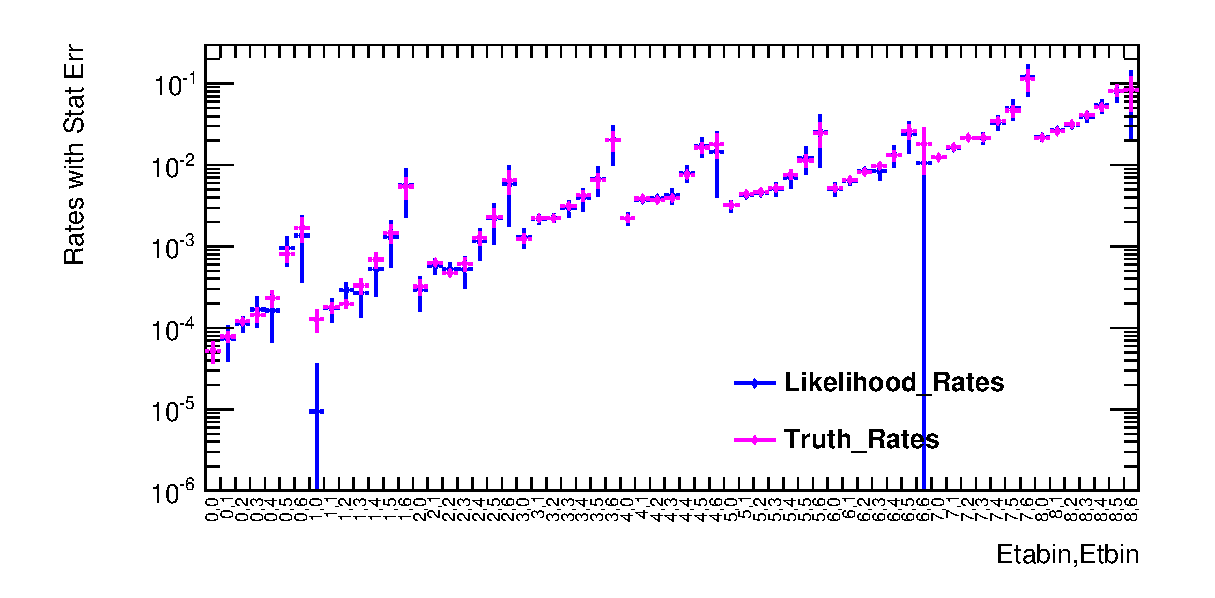
\includegraphics[width=0.8\textwidth]{figures/ChargeMisID/LL_TR_Com.eps}
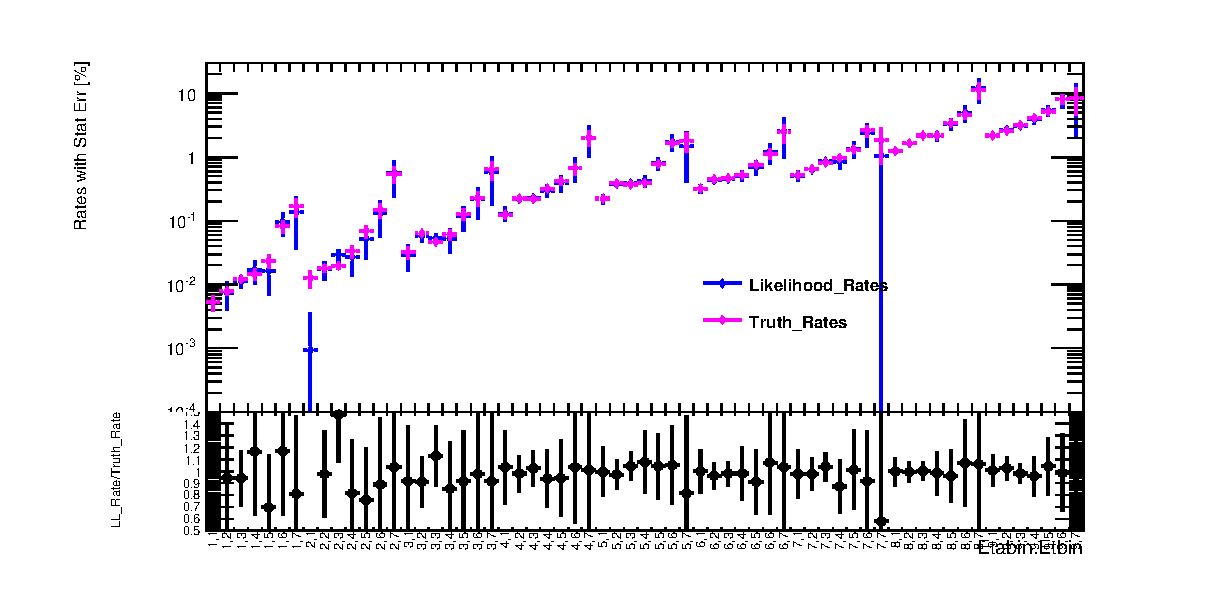
\includegraphics[width=0.8\textwidth]{figures/ChargeMisID/LL_TR_Com_new.eps}

\caption{Comparisons of the charge misID rates obtained with the likelihood method and the truth method. The two sets of rates shown here were both measured with the same \Zee\ MC sample.
Statistical errors are shown. The $x$ axis label is
  the $|\eta|$, \pt\ bin index, as defined in Table~\ref{tab:Etbin and Etabin of mis-charge rate}.}
  
% This is mis-charge rate comparison between likelihood and
%   truth method considering statistic errors. The two sets of rates
%   here are both measured with \Zee\ MC samples. The $x$ axis label is
%   the \eta, \pt\ bin index.}
\label{fig:LL_Truth_Comparison}
\end{figure}  

% Through the comparison, one can see that the rates measured with the
% likelihood method are compatible with that obtained with the truth
% method. The difference between these two sets of rates is taken into account as a systematic in the final measurement.
%

 % \subsubsection{Estimation of the charge misID rates in the data}


The misID rates measured in data using the likelihood method are shown in Figure~\ref{fig:LL_Rates_Egamma}.

% The likelihood method is then applied in the data to measure the charge misID rates.
%  % using the skimmed data from Egamma stream.
% % in Egamma stream we measure the data-driven rates with
% % (\texttt{user.along528.data12\_8TeV.period*.physics\_EGamma.PhysCont.NTUP\_SMWWW.SMN2N\_2\\Lep\_v1\_EXT0}
% % where * is A,B,C,D,E,G,H,I,J,L. These samples are slimmed with loose
% % di-lepton requirement, the di-lepton slim require there are at least 2
% % tagged high \pt\ leptons where tagged high \pt\ means Electron/Muon
% % satisfies any object quality requirement (loose, medium or tight for
% % muons and loose++,\\medium++,tight++,
% % veryLooseLL,looseLL,mediumLL,tightLL, or veryTightLL for electrons)
% % and has a pt of at least 10 GeV.).
%
% They are measured using the same selection described above. This estimation is used as the central value for the charge misID rates measurement. Figure~\ref{fig:LL_Rates_Egamma}, show the central value of the rate and their statistical error as a function of the $|\eta|$ and \pt\ bin index defined in Table~\ref{tab:Etbin and Etabin of mis-charge rate}.

% They are shown as a function of the \eta and \pt\ bin index defined in Table~\ref{tab:Etbin and Etabin of mis-charge rate}, in Figure~\ref{fig:LL_Rates_Egamma}.


\begin{figure}[htp]
\centering
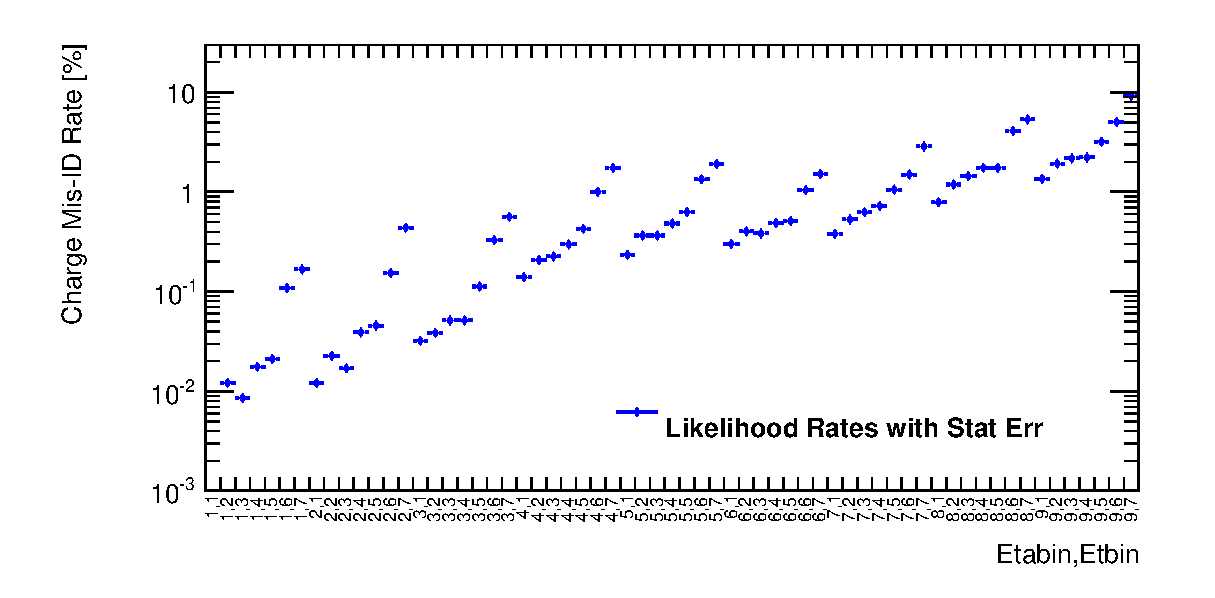
\includegraphics[width=0.8\textwidth]{figures/ChargeMisID/Egamma_LLB_new.eps}
\caption{Electron charge misID rates obtained from data with the likelihood method. Statistical errors are shown. The $x$ axis label is
  the $|\eta|$, \pt\ bin index, as defined in Table~\ref{tab:Etbin and Etabin of mis-charge rate}.}

% This is electron mis-charge rates measured from data with likelihood method and its statistic errors. Label on x axis is \eta, \pt\ bin indices.}
\label{fig:LL_Rates_Egamma}
\end{figure}


 \subsubsection{Systematic effect on charge misID rates due to background contamination}

The contamination of non-$Z\rightarrow{}ee$ processes in the previous selection is taken into account as a systematic.

In order to study this effect, a template fit approach is used. The signal template is obtained from the same MC simulation sample used above, while the background template is obtained from a looser data selection enriched in background events. Due to statistic constraints the background template is obtained in each $|\eta|$ bins, but the $\pt$ bins are grouped together. The event selection for the background template request the presence of a good isolated electron as defined in Section~\ref{sec:Object_selection}, and a second electron failing the tight++ identification cut. 

The two templates are then used on the invariant mass distribution of the electron pairs, in each $\pt$ and $|\eta|$ bins to determine the background contribution, subtract it and recompute the rate by maximizing the likelihood defined in Eq.~(\ref{eq:lnL_chargeMisID}). The difference between this new set of rates and the central value is then taken as a systematic uncertainty on the method, and are summarized in Table~\ref{tab:Charge_MisID_Bkg_Sys}. Further details on this method are also provided in Appendix~\ref{sec:appendix_chargeMisID}.

% The uncertainty due to the background contamination is summarized in Table~\ref{tab:Bkg Sys}.

% We estimate the background effect with
% coarser binning and include the shift in mischarge rate in the
% systematics.


%  We apply the likelihood method and event selection mentioned before
%  to data and we get the data-driven electron mis-charge rates, but
%  the rates are measured from data so there will be background events
%  remaining in the selected events. We use those rates directly
%  measured from data as central values and then subtract the
%  background contribution in the rates, we can calculate another set
%  of likelihood rates using the events without background, we may
%  call those rates clean rates. The difference between central values
%  and clean rates is the background systematic.



\begin{table}
\footnotesize
\centering
\begin{tabular}{c|c|c|c|c|c|c|c|c|c}
  \hline
  \backslashbox{\pt[\GeV]}{$|$\eta$|$} &[0,0.8] &[0.8,1.15] &[1.15,1.60] &[1.60,1.80] &[1.80,2.0] &[2.0,2.20] &[2.20,2.30] &[2.30,2.40] &[2.40,2.50] \\ 
  \hline
  [15,30] &8.85 &5.63 &5.75 &5.85 &5.79 &5.64 &5.64 &5.68 &5.49 \\
  \hline
  [30,40] &5.73 &5.71 &5.83 &5.97 &5.75 &5.78 &5.72 &5.81 &5.59 \\
  \hline
  [40,50] &5.76 &5.69 &5.71 &5.71 &5.65 &5.71 &5.62 &5.71 &5.62 \\
  \hline
  [50,60] &5.74 &5.55 &5.64 &5.53 &5.61 &5.65 &5.41 &5.49 &5.65 \\
  \hline
  [60,80] &5.77 &5.57 &5.71 &5.99 &5.59 &5.66 &5.35 &5.53 &5.41 \\
  \hline
  [80,120] &5.79 &5.63 &5.73 &5.71 &5.74 &5.77 &5.36 &5.74 &5.89 \\
  \hline
  [120,1000] &5.76 &5.71 &5.54 &5.76 &5.52 &5.61 &5.73 &5.98 &6.14  \\
  \hline
\end{tabular}
\caption{Systematic uncertainties on the central value charge misID rates expressed in percent. These uncertainties were obtained considering the impact of the background contamination in the selection.}
% Numbers here are background systematics over central values
%   in percent.}
\label{tab:Charge_MisID_Bkg_Sys}
\end{table} 
 


\subsubsection{Final rates}

The rates with the final errors used in the analysis are shown in Figure~\ref{fig:ChargeMisID_truthRate_finalFig}. The total systematic uncertainty is obtained doing a quadratic sum of the error obtained comparing the MC likelihood method and the truth method, shown in Table~\ref{tab:MCLLTruthSys}, and the error obtained considering the background contamination in the selection. The rates are also given in Table~\ref{tab:LL_finalRates}.

 \begin{figure}[htp]
 \centering
 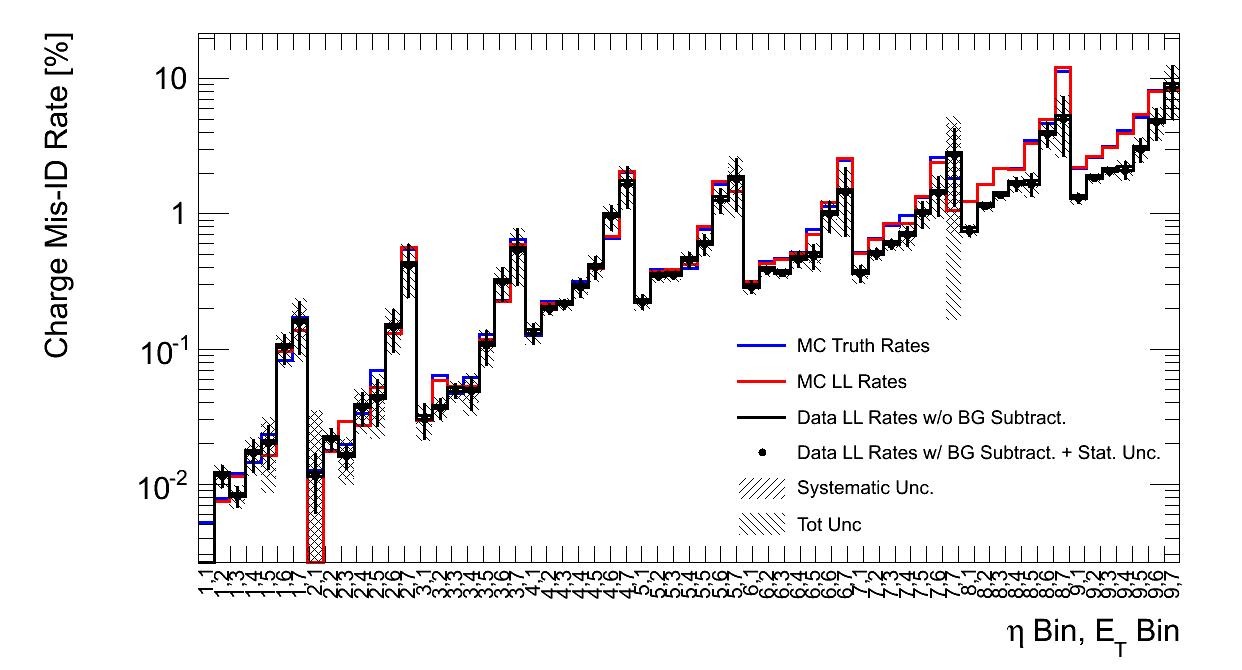
\includegraphics[width=0.8\textwidth]{figures/ChargeMisID/Validation_ChargeMisIDRates_PTvsEta_FinalRateWithSys.png}
 \caption{Electron charge misID rates obtained from data with the likelihood method. All the errors are now shown. The $x$ axis label is
  the $|\eta|$, \pt\ bin index, as defined in Table~\ref{tab:Etbin and Etabin of mis-charge rate}.}
 \label{fig:ChargeMisID_truthRate_finalFig}
 \end{figure}

\begin{table}
\footnotesize
\centering
\begin{tabular}{c|c|c|c|c|c|c|c|c|c}
  \hline
  \backslashbox{\pt[\GeV]}{$|$\eta$|$} &[0,0.8] &[0.8,1.15] &[1.15,1.60] &[1.60,1.80] &[1.80,2.0] &[2.0,2.20] &[2.20,2.30] &[2.30,2.40] &[2.40,2.50] \\
  \hline
  [15,30] & $> 100$ & $> 100$ &9.24 &3.12 &0.70 &0.05 &2.27 &0.25 &0.80 \\
  \hline
  [30,40] & 5.98 &2.58 &9.91 &2.14 &2.97 &3.84 &2.51 &0.63 &2.44\\
  \hline
  [40,50] & 6.22 &32.26 &11.36 &2.19 &4.12 &2.17 &3.52 &0.43 &2.13 \\
  \hline
  [50,60] & 14.22 &22.92 &17.20 &6.72 &7.13 &2.08 &14.80 &1.75 &4.52 \\
  \hline
  [60,80] & 43.45 &32.03 &9.39 &6.14 &3.93 &9.86 &1.19 &4.22 &3.84 \\
  \hline
  [80,120] & 14.59 &12.57 &2.51 &3.14 &4.73 &6.90 &9.40 &6.40 &1.34 \\
  \hline
  [120,1000] & 23.46 &3.02 &9.53 &1.02 &22.98 &3.17 &73.12 &5.61 &3.31 \\
  \hline
\end{tabular}
\caption{The absolute value of the difference between the charge mis-identification rates derived in MC using the truth method and using the likelihood method.  Numbers
are shown as a percent of the MC likelihood method.  These are transported to the likelihood rates in data and used as a systematic. }
\label{tab:MCLLTruthSys}
\end{table}



\begin{table}
\footnotesize
\centering
\begin{tabular}{c|c|c|c|c|c|c|c|c|c}
  \hline
  \backslashbox{\pt[\GeV]}{$|$\eta$|$} &[0,0.8] &[0.8,1.15] &[1.15,1.60] &[1.60,1.80] &[1.80,2.0] &[2.0,2.20] &[2.20,2.30] &[2.30,2.40] &[2.40,2.50] \\
  \hline
  $ \times 10^{}$
  [15,30] &$1.7370\times 10^{-11}$ &$9.4036\times 10^{-6}$ &0.0003 &0.0013 &0.0022 &0.0032 &0.0051 &0.0124 &0.0219\\
  \hline
  [30,40] &$7.4276\times 10^{-5}$ &0.0002 &0.0006 &0.0022 &0.0038 &0.0043 &0.0064 &0.0165 &0.0268 \\
  \hline
  [40,50] &0.0001 &0.0003 &0.0005 &0.0023 &0.0039 &0.0046 &0.0085 &0.0218 &0.0311 \\
  \hline
  [50,60] &0.0002 &0.0003 &0.0005 &0.0030 &0.0042 &0.0051 &0.0085 &0.0213 &0.0394 \\
  \hline
  [60,80] &0.0002 &0.0005 &0.0012 &0.0040 &0.0080 &0.0070 &0.0134 &0.0332 &0.0540 \\
  \hline
  [80,120] &0.0009 &0.0013 &0.0023 &0.0068 &0.0172 &0.0122 &0.0239 &0.0497 &0.0810 \\
  \hline
  [120,1000] &0.0014 &0.0056 &0.0059 &0.0204 &0.0147 &0.0255 &0.0106 &0.1208 &0.0820  \\
  \hline
\end{tabular}
\caption{Electron charge mis-ID rates, obtained with the likelihood method on the data.}
\label{tab:LL_finalRates}
\end{table}




Although the likelihood method, which is used to determined the rates from the data, was validated in MC using the truth method, it is quite important to validate the rates as much as possible, and to verify that if there are remaining differences they are covered within the systematic uncertainties that were assigned.

%As already stated, the charge misID rates are particularely important for the determination of the $WZ$ and $ZZ$ background contamination in the 0SFOS region. Therefore two more tests are conducted to test their validity.

We performed a test to recompute the charge misID rates using the truth method and a $WZ$ MC sample, and compare these new rates to the old one obtained with the $Z\to{}ee$ events. In principle, the charge misID is mostly due to detector effects, and it is therefore not expected to see any differences using one physics process or another one, as long as the GEANT4 geometry of the detector that was used to generate the events is the same. To perform this study, given the lower statistic available in the $WZ$ MC sample a different binning is used, it is summarized in Table~\ref{tab:Etbin and Etabin of mis-charge rate for WZ comparisons}. The new rates obtained are compared in Figure~\ref{fig:ChargeMisID_truthRate_Zee_WZ}. In this figure only the statistical error of each measurement is shown. A very good agreement between the two sets of rates is observed.



\begin{table}[htp]
\centering

\begin{tabular}{c|c||c|c}
	 \hline
	  $|\eta|$ bins & $|\eta|$ bin index   & \pt\ bins [\GeV] & \pt\ bin index \\
 	 \hline
	  $[0, 1.15]   $   & 0 	   &  $[15, 40]$ & 0 \\
	  $[1.15, 1.8] $   & 1 	   &  $[40, 60]$ & 1 \\
	  $[1.8, 2.2] $   & 2	   &  $[60, 100]$ & 2 \\
	  $[2.2, 2.5] $   & 3 	   &  $[100, 1000]$ & 3 \\

  \hline
\end{tabular}
\caption{The $|\eta|$ and \pt\ bins used for the comparison of mischarge
  rate obtained with MC $Z\to{}ee$ sample and MC $WZ$ sample. The bin index used in the 1D figures~\ref{fig:ChargeMisID_truthRate_Zee_WZ} are given.}
\label{tab:Etbin and Etabin of mis-charge rate for WZ comparisons}
\end{table}



 \begin{figure}[htp]
 \centering
 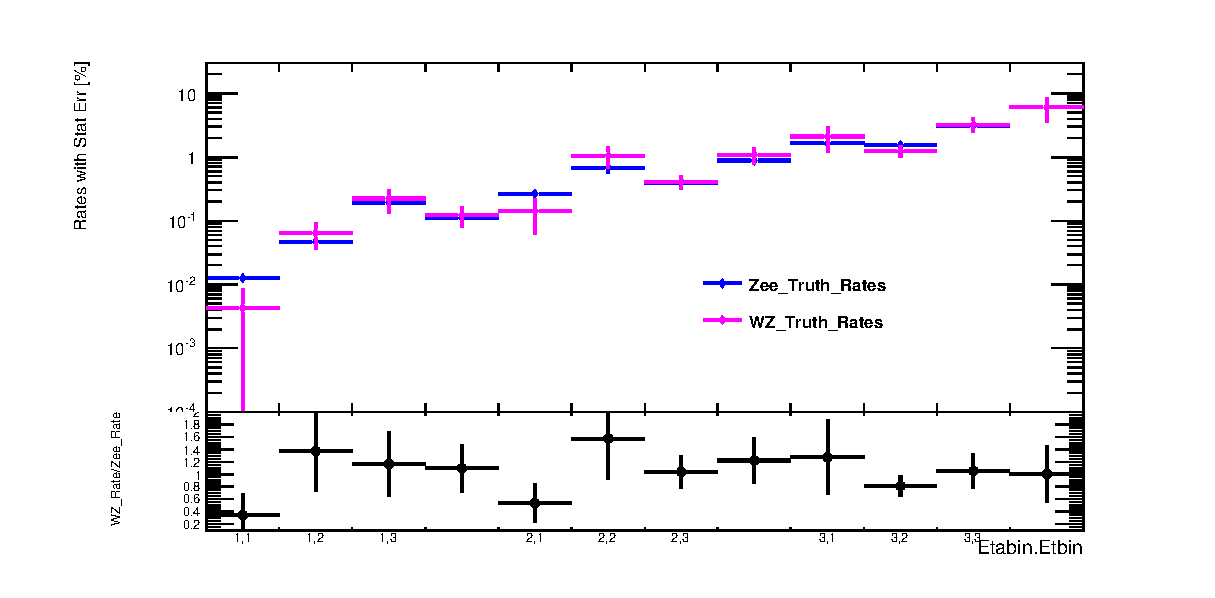
\includegraphics[width=0.8\textwidth]{figures/ChargeMisID/Validation_ChargeMisIDRates_PTvsEta_CompareSSRate.eps}
 \caption{Electron charge misID rates obtained from MC $Z\to{}ee$ with the likelihood method are compared with rates obtained using the truth method in a MC $WZ$ sample. Errors shown here are purely statistics. The $x$ axis label is
  the $|\eta|$, \pt\ bin index, as defined in Table~\ref{tab:Etbin and Etabin of mis-charge rate for WZ comparisons}.}
 \label{fig:ChargeMisID_truthRate_Zee_WZ}
 \end{figure}


\subsubsection{Application and validation of rates}
As already stated, the charge misID rates are primarily important for the determination of the $WZ$ and $ZZ$ background contamination in the 0SFOS region. 
Once derived, the rates are applied to $WZ$ and $ZZ$ MC samples based on whether or not a charge flip could cause the event to appear in the 0 SFOS region.  
In particular, the following di-boson decays are considered:
\begin{itemize}
\item $WZ\rightarrow e^{\pm}\nu~ e^{+}e^{-}$
\item $WZ\rightarrow \mu^{\pm}\nu~ e^{+}e^{-}$
\item $WZ\rightarrow \tau^{\pm}\nu~ e^{+}e^{-}$
\item $ZZ\rightarrow e^{+}e^{-}~e^{+}e^{-}$
\item $ZZ\rightarrow \mu^{+}\mu^{-}~ e^{+}e^{-}$
\end{itemize}
No other decay channels are considered.  These all share in common that they have at least one electron-positron pair.  
Except for the $WZ\rightarrow \tau^{\pm}\nu~e^{+}e^{-}$ decay channel, decay channels with tau leptons are not considered
because they are suppressed by the tau branching fraction and are considered to be negligible.

The charge mis-identification rates are then applied to these channels on an event-by-event basis as follows.
For each event that is processed, its decay channel is identified at truth level. Each reconstructed lepton
is examined  and assigned a rate, or a probability to charge flip, based on its reconstructed $\pt$ and $\eta$ values.
The probability for a charge flip to occur in an event is then approximately the sum of rates for the individual electrons:
\begin{equation}
\textrm{Probability of Charge Mis-Identification in Event} = \sum_{i \in \textrm{Electrons}}  \textrm{Rate}(\pt^i,\eta^i) + \textrm{Higher Order Terms}
\end{equation}
Higher order terms where multiple electrons are charge mis-identified is small and considered to be negligible.
We are only concerned with the probability that a charge flip results in the event falling into the 0 SFOS region. 
Consider a step function, $\Theta(e)$, defined for an individual event:
\[
\Theta(e) = 
\begin{cases}
\hfill 1 \hfill & \text{if flipping charge of $e$ classifies event as 0 SFOS} \\
\hfill 0 \hfill & \text{if flipping charge of $e$ does NOT classify event as 0 SFOS}\\
\end{cases}
\]
Then the probability that a charge mis-identification occurs and results in the event falling in the 0 SFOS region is:
\begin{equation}
\textrm{Probability that event is classified as 0 SFOS} = \sum_{i \in \textrm{Electrons}}  \textrm{Rate}(\pt^i,\eta^i)\Theta(i) + \textrm{Higher Order Terms}
\end{equation}
Again, we ignore the case where multiple electrons have their charge mis-identified.  
This probability is then used as an event by event weight. 



Once the weight has been determined, we then artificially flip the charge of one of the electrons/positrons in the event.
If there is only one electron in the event that will lead the event to fall in the 0 SFOS region, its charge is flipped
and one proceeds to the next event.  However, if there are multiple electrons in the event, there is an ambiguity that must be resolved
about which electron's charge should be flipped. One must then be careful in this case to not introduce any bias.
We decided to choose a procedure where we pick a single electron from the event at random based on the charge flip rates
of the individual electrons. Thus, for an individual electron in an event, the probability that it is chosen to have its charge
flipped is:
\begin{equation}
\textrm{Probability that $e$ has charge flipped} = \textrm{Rate}(\pt^e,\eta^e)\Theta(e)~/\sum_{i \in \textrm{Electrons}} \textrm{Rate}(\pt^i,\eta^i)\Theta(i)
\end{equation}

Consider an example 
where the event under consideration comes from the decay $WZ\rightarrow e^{+}\nu e^{+}e^{-}$. Assume all three charged leptons pass reconstruction and are selected then label them as: $e^{+}_1~e^{+}_2e^{-}_3$. In this case,
the only way that this event could be classified as 0 SFOS when flipping the charge of only one electron/positron is to flip the charge of the electron.
Thus, $\Theta(e^{+}_1)=\Theta(e^{+}_2)=0$ and $\Theta(e^{-}_3)=1$.  The event weight will then be equal to the rate of charge mis-identification for  $e^{-}_3$ and it
will have it's charge flipped to be positive.

Now consider an example of an event with the decay of $ZZ\rightarrow \mu^{+}\mu^{-}~ e^{+}e^{-}$.
If all four leptons are reconstructed and selected, the event will not be considered at all in the three lepton selection of this analysis, so consider the 
case where the $\mu^{+}$ is not selected leaving three leptons labeled as: $\mu^{-}_1 e^{+}_2 e^{-}_3$.  The probability for the muon to charge flip
is negligible which leaves the electron and the positron. Flipping the charge of either one at a time will result in the event being classified as 0 SFOS.  Thus, in
this case $\Theta(\mu^{-}_1)=0$ and $\Theta(e^{+}_2)=\Theta(e^{-}_3)=1$. The event weight will then be the sum of the rates for $e^{+}_2$ and $e^{-}_3$.
The probability that the electron has its charge flipped is then $\frac{\textrm{Rate}(e^{-}_3) }{ \textrm{Rate}(e^{+}_2)+ \textrm{Rate}(e^{-}_3)}$ and similarly for the positron.

This procedure has been validated on the $WZ$ and $ZZ$ samples by comparing the predictions taken directly from MC to the predictions reweighted in the 0 SFOS signal region using the procedure just described. This is done in Figure~\ref{fig:ChargeMisID_Validation_WZ} for the $WZ$ samples and on Figure~\ref{fig:ChargeMisID_Validation_ZZ} for the $ZZ$ samples. It can be seen the agreement in the shape looks good for all the distributions. An offset between the two distributions is observed. This difference is covered partially by the systematic uncertainties of the method.  Any remaining difference could be expected from the difference in rates observed at high $\eta$ and high $E_{T}$ as seen in Fig.~\ref{fig:ChargeMisID_truthRate_finalFig} and serves as justification for using the data-driven method.

There is no special treamtent of the charge mis-identification contribution to other background contributions in the 0 SFOS region or to any contributions to the 
1 and 2 SFOS signal regions, including diboson processes, as the effect is expected to be very small.  Any charge mis-identification events are thus taken directly 
from MC in this case.


 \begin{figure}[htp]
 \centering
 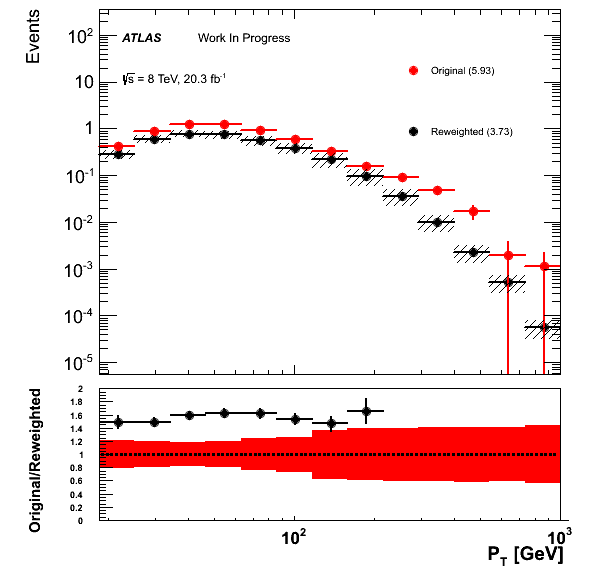
\includegraphics[width=0.4\textwidth]{figures/ChargeMisID/Validation_ChargeMisIDRates_WZ_PTLepton.png}
 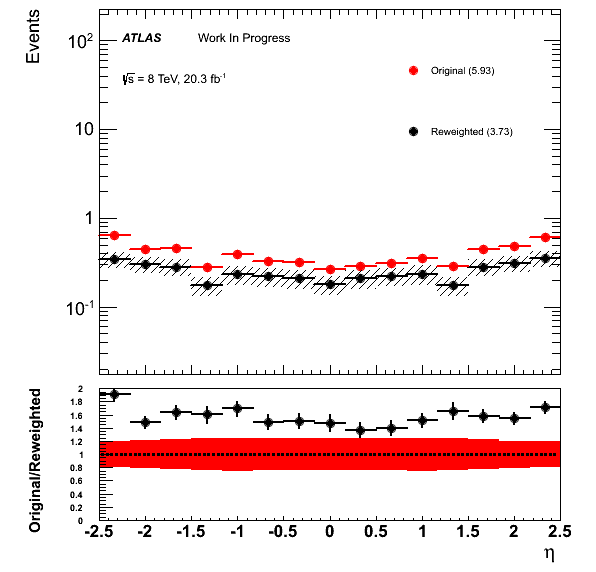
\includegraphics[width=0.4\textwidth]{figures/ChargeMisID/Validation_ChargeMisIDRates_WZ_EtaLepton.png}
 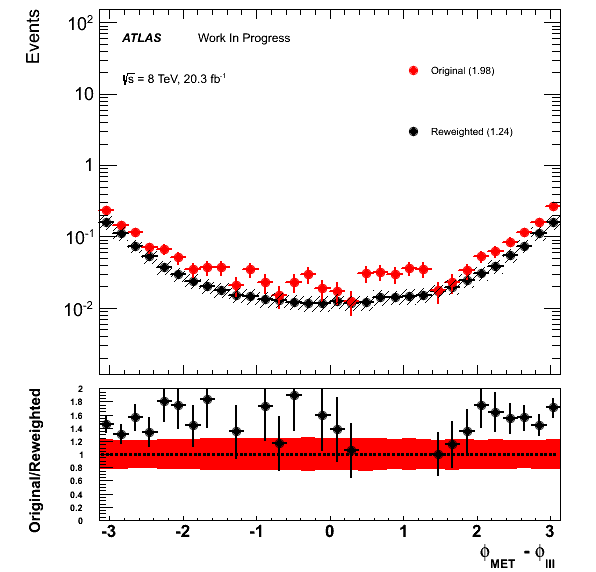
\includegraphics[width=0.4\textwidth]{figures/ChargeMisID/Validation_ChargeMisIDRates_WZ_DeltaPhi.png}
 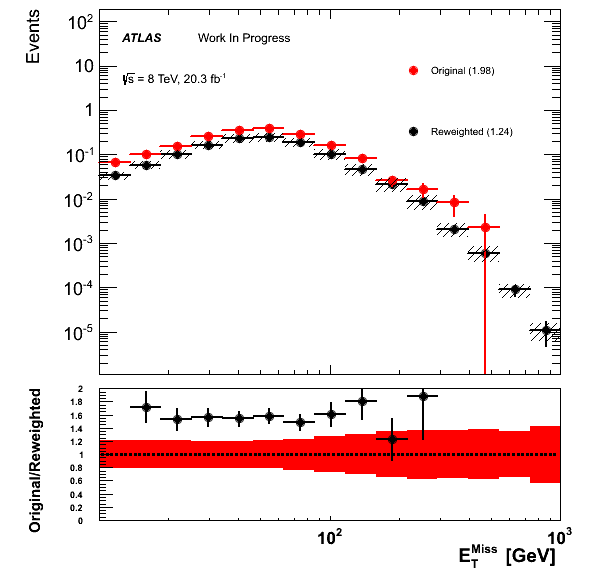
\includegraphics[width=0.4\textwidth]{figures/ChargeMisID/Validation_ChargeMisIDRates_WZ_MET.png}
 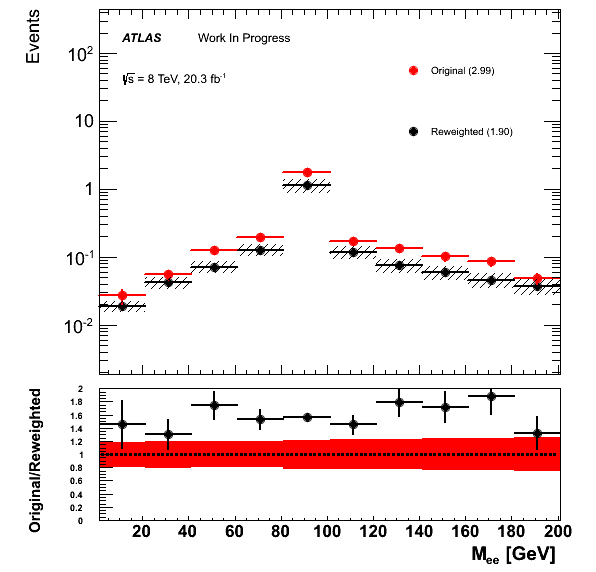
\includegraphics[width=0.4\textwidth]{figures/ChargeMisID/Validation_ChargeMisIDRates_WZ_Mee.png}
 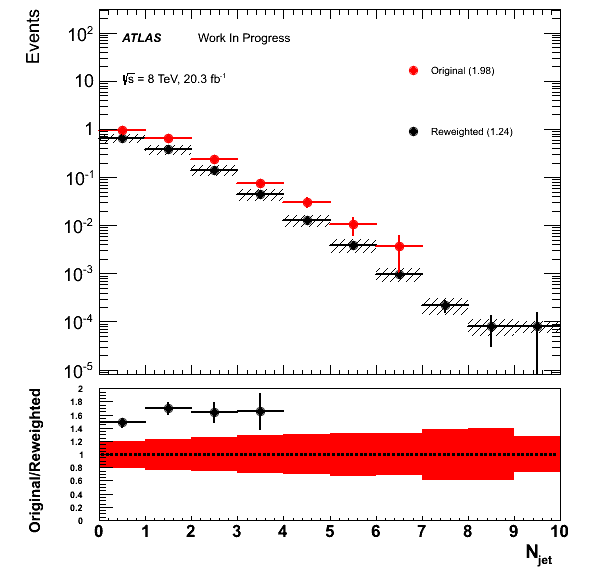
\includegraphics[width=0.4\textwidth]{figures/ChargeMisID/Validation_ChargeMisIDRates_WZ_JetMultiplicity.png}

 \caption{Validation of the charge mis-ID rates comparing MC $WZ\rightarrow \ell ee$ ($\ell=e,\mu$) samples reweighted with the charge misID rates measured in the MC $Z\to{}ee$ 
 sample to the original MC predictions. Distribution of lepton $p_{T}$, $\eta$, $\Delta \phi(3l,E_{T}^{Miss})$,\met{}, Same-sign di-electron invariant mass, and jet multiplicity.}
 \label{fig:ChargeMisID_Validation_WZ}
 \end{figure}
 
 
 \begin{figure}[htp]
 \centering
 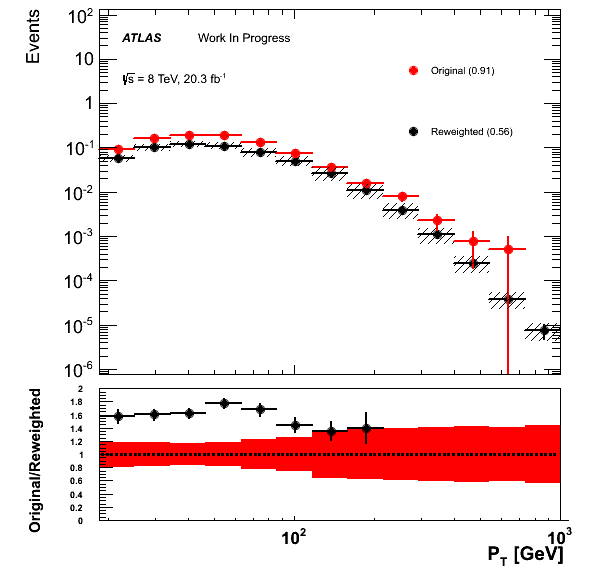
\includegraphics[width=0.4\textwidth]{figures/ChargeMisID/Validation_ChargeMisIDRates_ZZ_PTLepton.png}
 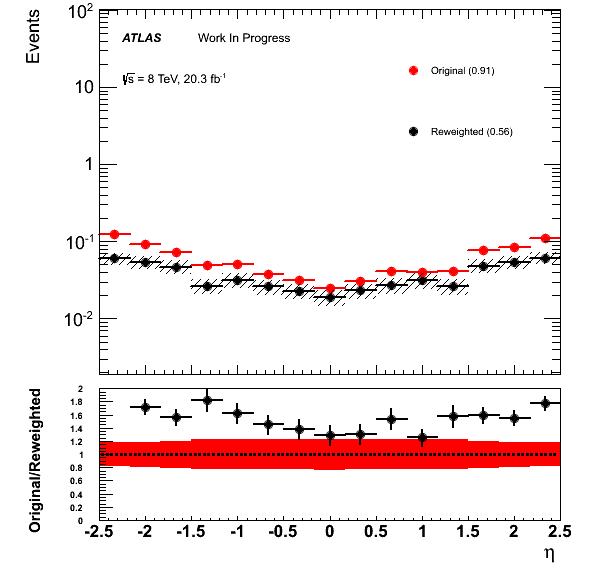
\includegraphics[width=0.4\textwidth]{figures/ChargeMisID/Validation_ChargeMisIDRates_ZZ_EtaLepton.png}
 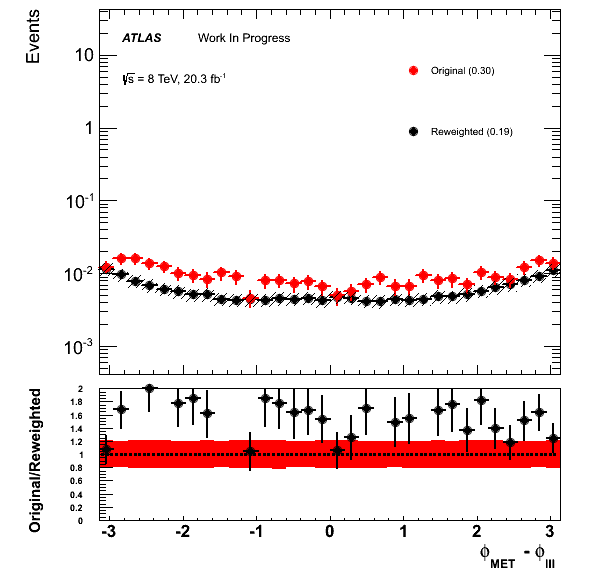
\includegraphics[width=0.4\textwidth]{figures/ChargeMisID/Validation_ChargeMisIDRates_ZZ_DeltaPhi.png}
 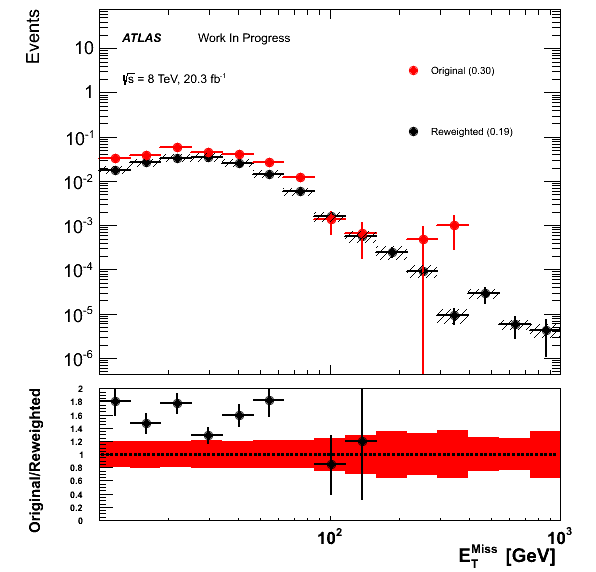
\includegraphics[width=0.4\textwidth]{figures/ChargeMisID/Validation_ChargeMisIDRates_ZZ_MET.png}
 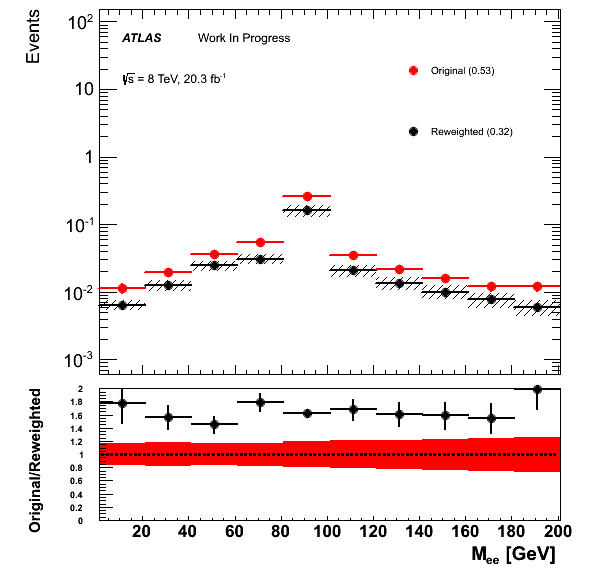
\includegraphics[width=0.4\textwidth]{figures/ChargeMisID/Validation_ChargeMisIDRates_ZZ_Mee.png}
 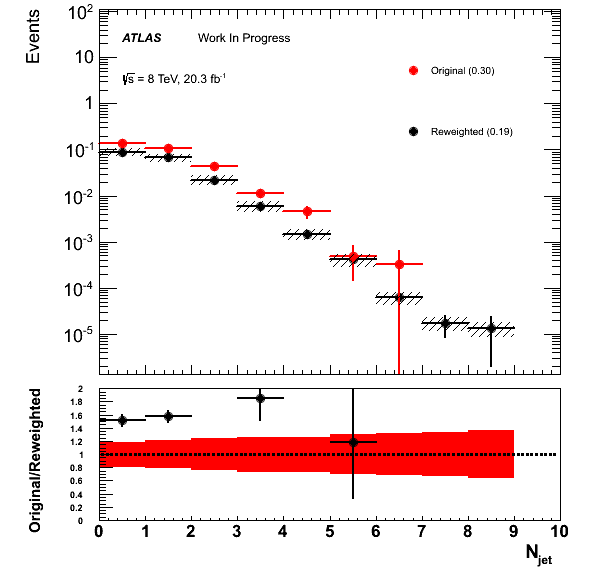
\includegraphics[width=0.4\textwidth]{figures/ChargeMisID/Validation_ChargeMisIDRates_ZZ_JetMultiplicity.png}

 \caption{Validation of the charge mis-ID rates comparing MC $ZZ\rightarrow \ell \ell ee$ ($\ell=e,\mu$) samples reweighted with the charge misID rates measured in the MC $Z\to{}ee$ 
 sample to the original MC predictions. Distribution of lepton $p_{T}$, $\eta$, $\Delta \phi(3l,E_{T}^{Miss})$,\met{}, Same-sign di-electron invariant mass, and jet multiplicity.}
 \label{fig:ChargeMisID_Validation_ZZ}
 \end{figure}







\section{Background Estimates}
\label{sec:bg_estimates}

%
Details of the MC based background estimations are described below.
Any additional normalizations or uncertainties are summarized
in Table~\ref{tab:mcnorm}.

\begin{table}[htp]
\centering
    \begin{tabular}{|c|cc|}
    \hline
    Background & Normalization Factor & Unceratinty \\ 
    \hline\hline
    $WZ$ & 1.08 & 10~\% \\
    $ZZ$ & 1.05 & 15~\% \\
    %$Z\gamma$ & & 30~\% \\
    $\ttbar +V$ & 1.0 & 30~\% \\
    $ZWW+ZZZ$ & 1.0 & 50~\% \\
    \hline
  \end{tabular}
  

\caption{Summary of normalizations and their uncertainties for the
MC based background estimates used in the analysis.}
\label{tab:mcnorm}
\end{table}



\subsubsection{$WZ\rightarrow lll\nu$}
\label{sec:wzbg}

The $WZ\rightarrow lll \nu$ background is the most important prompt background 
to the $WWW$ signal process. Thus, it must be studied carefully.
The most recent measurements of the $WZ$ process at the LHC
\cite{Aad:2012twa,Anger:1663539,CMS-PAS-SMP-12-006} 
show some tension with the current NLO MC predictions for this process, 
with differences of about 10 to 15\%. 
Studies of other di-boson processes 
\cite{Grazzini:2015nwa,Cascioli:2014yka}
suggest that this could be resolved by 
moving to a NNLO calculation.
For the $WZ$ process, however, this type of calculation is not yet available.
As a result, we instead use the so-called ``2D Sideband'' method
\cite{Aad:2013izg} to derive a correction using the data itself.
This correction is applied to the $WZ$ background MC estimate using
\powheg~mentioned in \sec\ref{sec:www_bg_samples}.

The 2D sideband method is able to determine an estimate
for the process of interest using the data while also correcting
for background contamination. 
To do this, first a signal region 
is chosen which is enriched in the process of interest.
This signal region should have at least two 
independent selection requirements which when inverted suppress
the signal and enhance the backgrounds to that signal.
Next, by inverting one, the other, or both selection requirements, 
three different control regions can be formed
where the signal is suppressed and the backgrounds are enhanced 
with respect to the signal region. 
These control regions are referred to as ``sidebands''.
The three sidebands and the signal region may be
related to each other assuming independence of the two different selection
requirements. If this assumption holds, then the relative change in the 
backgrounds should be the same
when inverting one cut while keeping the other fixed, and vice-versa.
In this way, one may solve algebraically for the background contamination 
in the signal region and subtract it out, resulting in a pure
estimate of the signal from the data. 


In this case, the signal region is chosen to be enhanced in the $WZ$ process.
The backgrounds to this process are from electroweak contributions (like
$ZZ$, \ttV, and $VVV$) and from backgrounds with fake leptons.
The contributions to the signal region are thus parameterized as
\begin{equation}
\label{eq:wzparam}
N^{\textrm{Data}} =  N^{WZ} + N^{\textrm{Fake}} + N^{\textrm{Electroweak}}
\end{equation}
These backgrounds include processes without \z-bosons.
Thus, the presence of the \z-boson in the signal means that applying a \z-veto of 
$|m_{\textrm{SFOS}}-m_{\z}|<15\GeV$
will suppress these contributions to the background.
Also, requiring that the leptons be isolated does a good job of 
suppressing the fake background.
Thus, the same track and calorimeter isolation requirements
are applied to electrons and muons as in the $WWW$ signal regions
described in \sec\ref{sec:object_selection}.

%%%Do I want to show this figure?

%\begin{figure}[htp]
%\centering
%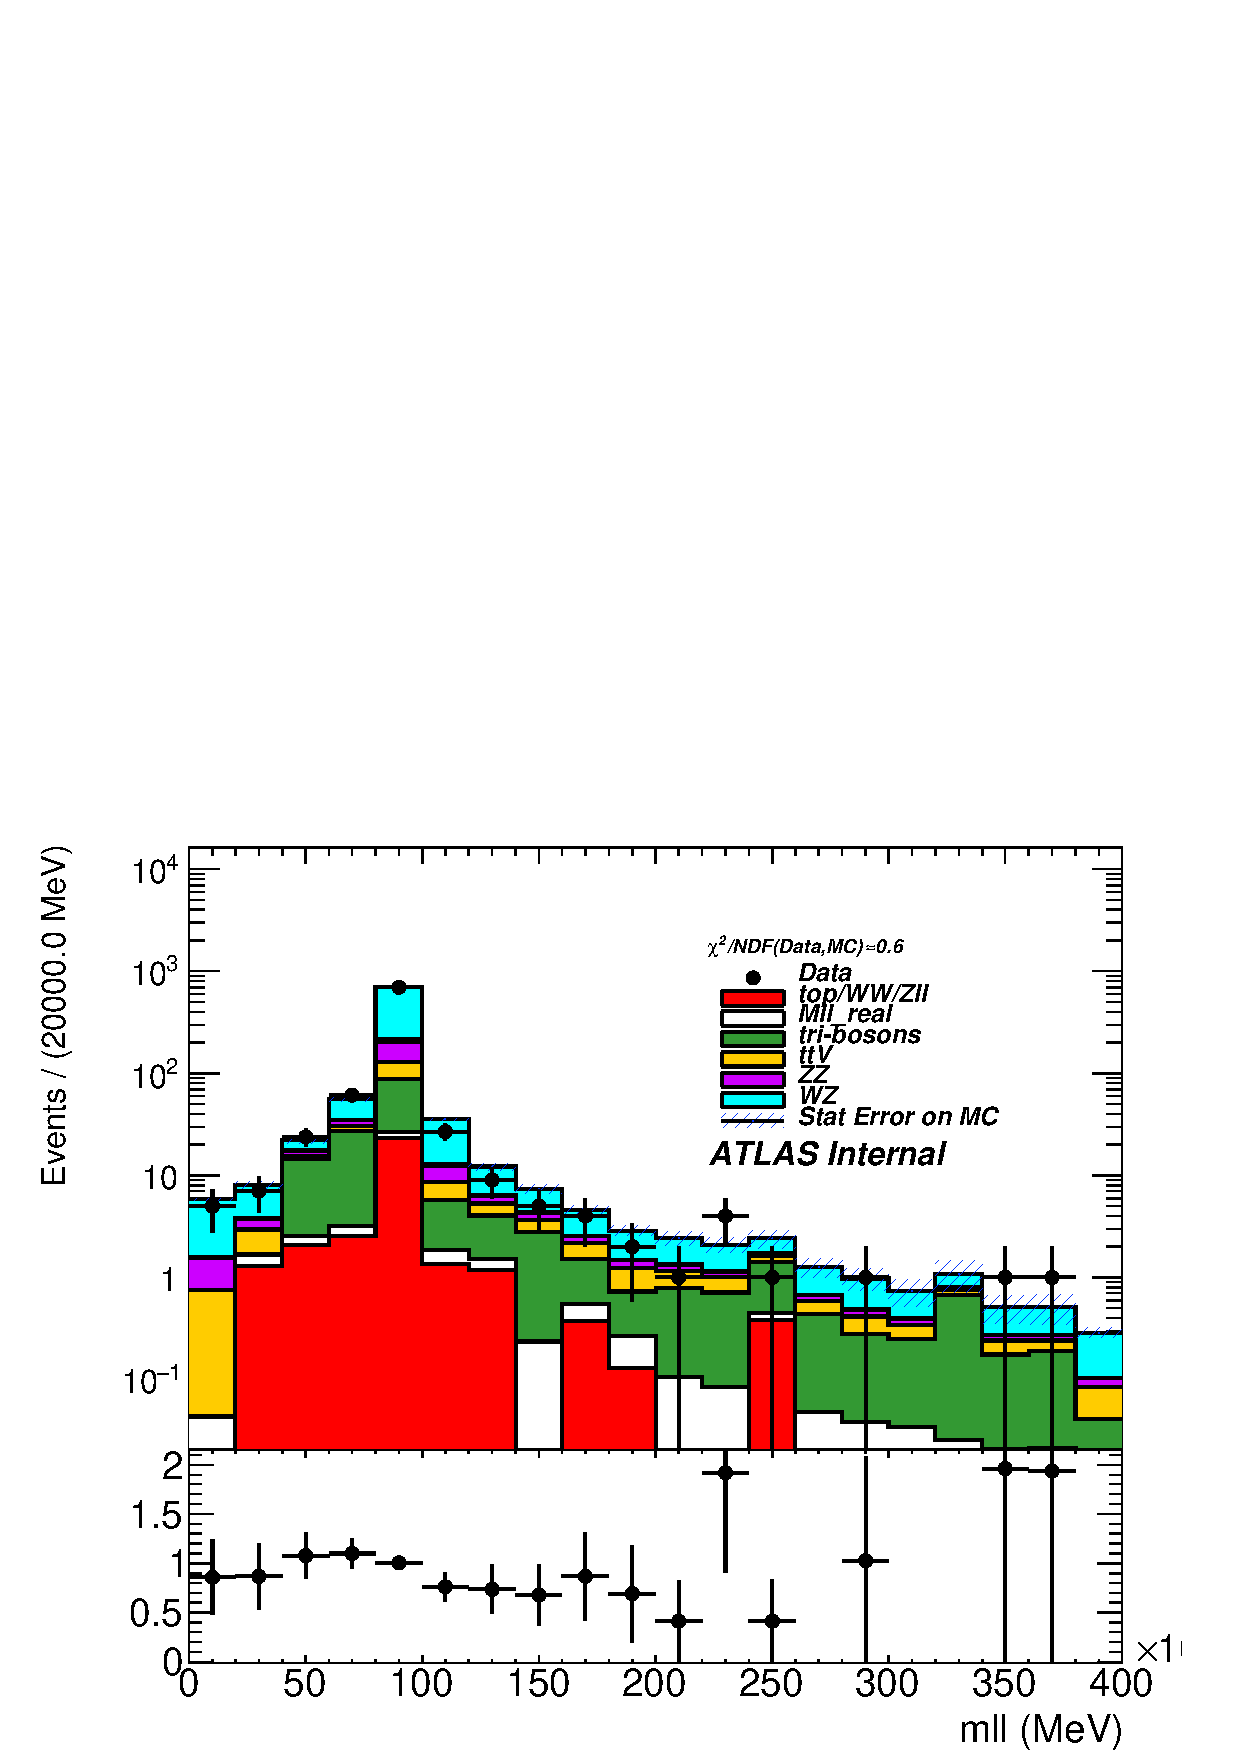
\includegraphics[width=0.45\textwidth]{figures/WZ_CR/2DSideband_WZCR_Isolated}
%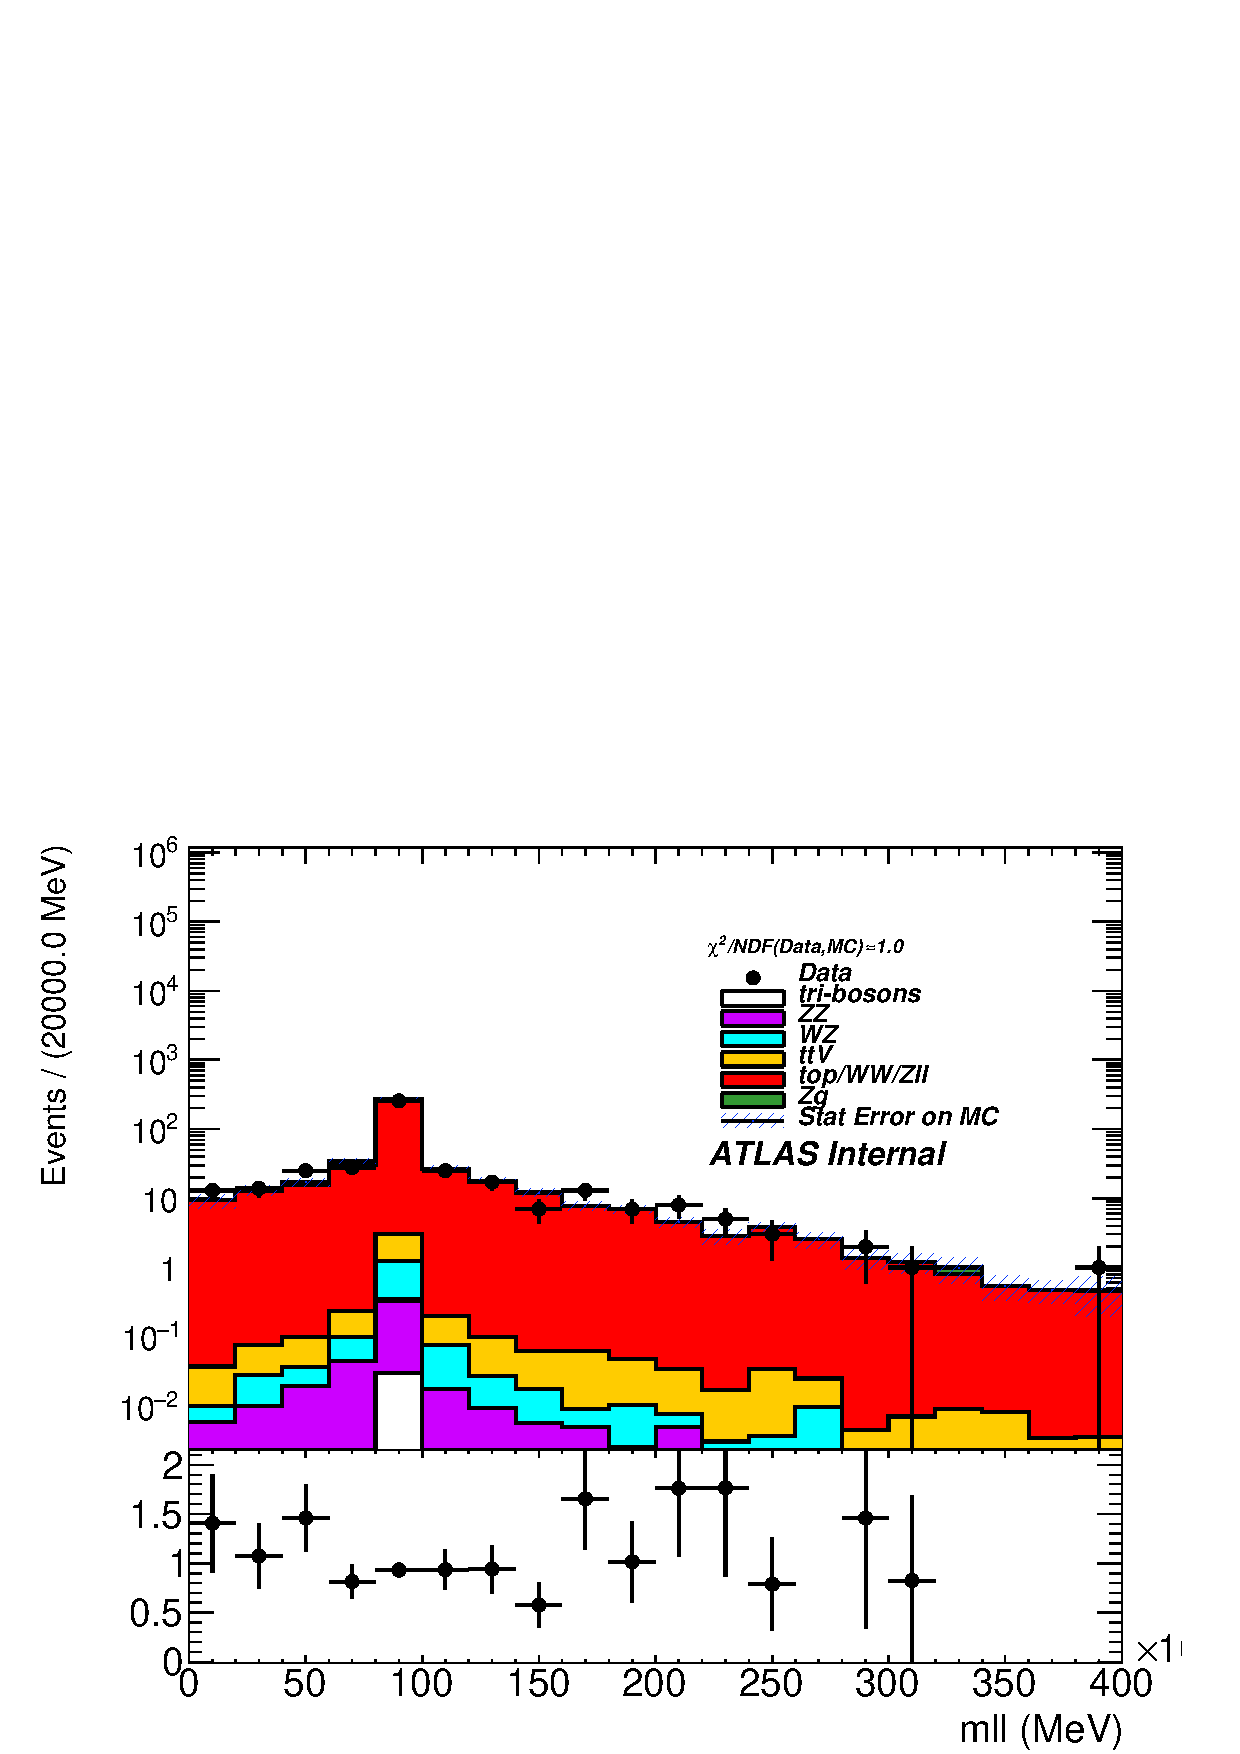
\includegraphics[width=0.45\textwidth]{figures/WZ_CR/2DSideband_WZCR_NonIsolated}
%\caption{ Distribution of $m_{\ell\ell}^{SFOS}$ in the isolated and  non-isolated 
%control regions. The agreement between the data and the MC expectation
%is not expected to be perfect, since the MC does not do a good job 
%of modeling the fake background. The 2D sideband method uses the data
%to estimate the fake background.}
%\label{fig:wz_sidebands}
%\end{figure}

The \z-veto and the isolation requirements are 
independently inverted\footnote{The thresholds are also slightly shifted 
so that there is a ``dead'' region between the signal regions and sidebands 
which is not used by either. This ensures separation between all regions.}
to form the three sidebands.
%The distribution of $m_{\textrm{SFOS}}$ is shown in
%\fig\ref{fig:wz_sidebands} in both the the isolated and non-isolated regions.
The expectation in each sideband can be parameterized
in the same way as \eqn\eqref{eq:wzparam}, resulting in one
equation for each region. By specifying the \z-veto condition
as $A$ and the isolation condition as $B$, \eqn\eqref{eq:wzparam}
can be rewritten as:
\begin{equation}
\label{eq:wzparam2}
N^{\textrm{Data}}_{A,B} =  N^{WZ}_{A,B} + N^{\textrm{Fake}}_{A,B} + N^{\textrm{Electroweak}}_{A,B}
\end{equation}
representing the four different equations after varying $A$ and $B$ indpendently.
For example, the signal region is when $A=\textrm{With \z-veto}$ and
$B=\textrm{Isolated}$.
One more equation can be found by assuming that the effect of 
the isolation cut on the fake background is independent of the \z-veto.
That is to say, it is assumed that:
\begin{equation}
\label{eq:wz_constraint}
R^{\textrm{Fake}}_{\textrm{With \z-veto}} = R^{\textrm{Fake}}_{\textrm{Without \z-veto}}
\end{equation}
where 
\begin{equation}
R^{\textrm{Fake}}_{A} = 
\frac{N^{\textrm{Fake}}_{A,\textrm{Isolated}}}
{N^{\textrm{Fake}}_{A,\textrm{Non-Isolated}}}
\end{equation}
This results in five equations: the expectations,
\eqn\eqref{eq:wzparam2}, from varying the conditions $A$ and $B$ independently,
and \eqn\eqref{eq:wz_constraint}.




If we can solve the equations above for $N^{WZ}_{A,B}$ in the signal region,
when $A=\textrm{With \z-veto}$ and $B=\textrm{Isolated}$,
then we have our estimate. 
This is 5 equations and 16 unnkowns. The four unknowns, $N^{\textrm{Data}}_{A,B}$,
are determined using the data directly while 
the electroweak backgrounds, $N^{\textrm{Electroweak}}_{A,B}$,
and the $WZ$ contributions in the sidebands, $N^{WZ}_{A,B}$ 
(when $A=\textrm{With \z-veto}$ and $B=\textrm{Isolated}$ are not both true)
are determined using $WZ$ MC. This reduces the problem to 5 equations
and 5 unknowns. Thus, we can solve algebraically for the remaining unkowns
including the desired value for the $WZ$ estimate in the signal region.

\begin{table}
\centering


\begin{tabular}{|cc|cc|}
\hline
%\multicolumn{3}{|c|}{$N^{\textrm{Data}}_{A,B}$}\\
\multirow{3}{*}{$N^{\textrm{Data}}_{A,B}$}&
\backslashbox{A}{B}& Isolated & Non-Isolated \\
\cline{2-4}
&With \z-veto & $724\pm27$ & $272\pm16$ \\
&Without \z-veto & $67\pm8$  & $118\pm11$ \\
\hline
\hline
%\multicolumn{3}{|c|}{$N^{\textrm{Electroweak}}_{A,B}$}\\
\multirow{3}{*}{$N^{\textrm{Electroweak}}_{A,B}$}&
\backslashbox{A}{B}& Isolated & Non-Isolated \\
\cline{2-4}
&With \z-veto & $172\pm3$ & $7.7\pm0.9$ \\
&Without \z-veto & $29\pm2$  & $1.9\pm0.6$ \\
\hline\hline
%\multicolumn{3}{|c|}{$N^{WZ}_{A,B}$ (MC)}\\
\multirow{3}{*}{$N^{WZ}_{A,B}$}&
\backslashbox{A}{B}& Isolated & Non-Isolated \\
\cline{2-4}
%&With \z-veto & $498\pm1$& $0.896\pm0.050$ \\
&With \z-veto & ---& $0.896\pm0.050$ \\
&Without \z-veto & $31.82\pm0.35$  & $0.095\pm0.015$ \\
\hline
\end{tabular}

\caption{All of the inputs used to constrain the system of five equations
from \eqn\eqref{eq:wzparam} and \eqn\eqref{eq:wz_constraint}.
The values are derived in the signal region and three sideband regions
described in the text. $N^{\textrm{Data}}_{A,B}$ are determined directly
from the data; $N^{\textrm{Electroweak}}_{A,B}$ and $N^{WZ}_{A,B}$ are 
determined in MC. The value for $N^{WZ}_{\textrm{With \z-veto,Isolated}}$ is
not used as an input and is instead solved for as the the main
parameter of interest. Still, the value is determined in MC to be
$498 \pm 1$.  Only statistical uncertainties are shown.}
\label{tab:wz_input}
\end{table}

\begin{table}
\centering


\begin{tabular}{|cc|cc|}
\hline
%\multicolumn{3}{|c|}{$N^{\textrm{Data}}_{A,B}$}\\
\multirow{3}{*}{$N^{\textrm{Fake}}_{A,B}$}&
\backslashbox{A}{B}& Isolated & Non-Isolated \\
\cline{2-4}
%&With \z-veto & $8\pm23$ &  \\ %this is the number provided by louis
&With \z& $14 \pm 43$ & $263\pm 16 $\\
&Without \z&  $6.2 \pm 8.3$ & $116 \pm 11$\\
\hline
\hline
\multirow{3}{*}{$N^{WZ}_{A,B}$}&
\backslashbox{A}{B}& Isolated & Non-Isolated \\
\cline{2-4}
&With \z& $537\pm35$ & --- \\ %I calculated 537.97 \pm 33.04
&Without \z& ---  & --- \\
\hline
\end{tabular}

\caption{Outputs from the system of five equations
from \eqn\eqref{eq:wzparam} and \eqn\eqref{eq:wz_constraint}
after including the numbers from \tab\ref{tab:wz_input} as input.
The value for $N^{WZ}_{\textrm{With \z-veto, Isolated}}$ is 
the value of primary interest.  Only statistical uncertainties are shown.}
\label{tab:wz_output}
\end{table}


The inputs to the system of equations are summarized in 
\tab\ref{tab:wz_input}\footnote{Note that the $WZ$ MC prediction in 
the signal region is not used except as a comparison.}.
The derived values after solving the system of equations are
summarized in \tab\ref{tab:wz_output}. 
The derived estiamte for the $WZ$ contribution to 
the signal region is 
$537 \pm 35$
events, where the uncertainty is purely statistical. 
Compare this to the estimate from MC of 
$498 \pm 1$ events.
The ratio of the two can be used to derive a k-factor of
$1.08\pm0.07\stat$.


Systematic uncertainties are also derived on the method
by varying the 
thresholds used to define the sideband regions, varying the normalization
of the MC estimates in \tab\ref{tab:wz_input}, and by varying the degree
of equality in \eqn\eqref{eq:wz_constraint}. The effect of each
uncertainty is propogated to the estimate of the $WZ$ normalization in
the signal region and are combined in quadrature. The total systematic
uncertainty is found to be 5.9\%. 
The final k-factor is thus $1.08 \pm0.07\stat\pm0.07\syst$.

The derived k-factor is applied to the MC estimate in another control
region enhanced in the $WZ$ process. This control region is determined
using the pre-selection region as described in \sec\ref{sec:preselection}
plus an additional requirement that there be 2 SFOS lepton pairs.
This gives a good test of the $WZ$ normalization in a control region
which is closer to the $WWW$ signal regions. 
The comparison is shown in \fig\ref{fig:WZ_2SFOS_CR} where
the data is shown to be in good agreement with the corrected $WZ$ MC
estimate, as desired.

\begin{figure}[htp]
\centering
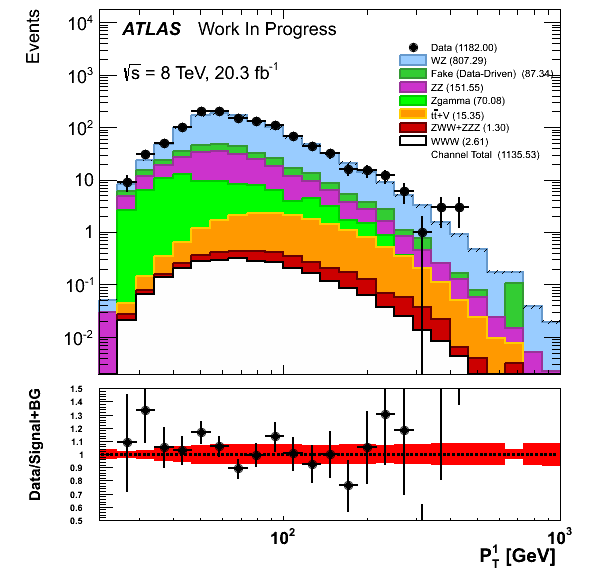
\includegraphics[width=0.4\textwidth]{figures/WZ_CR/LeadingLeptonPt_histratio.png}
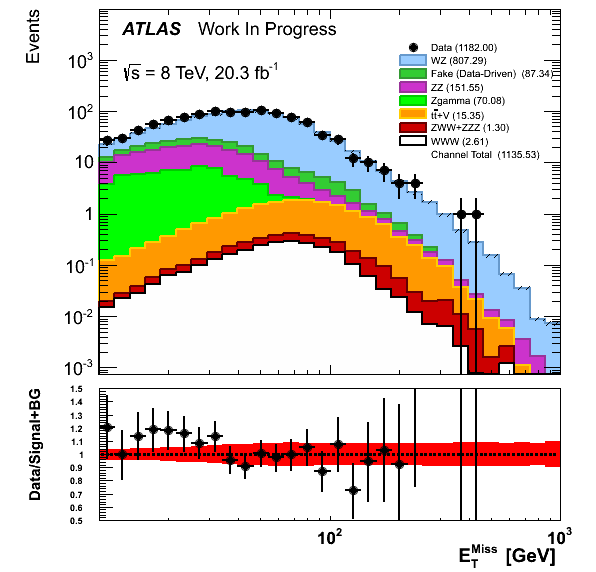
\includegraphics[width=0.4\textwidth]{figures/WZ_CR/MET_Et_histratio.png}
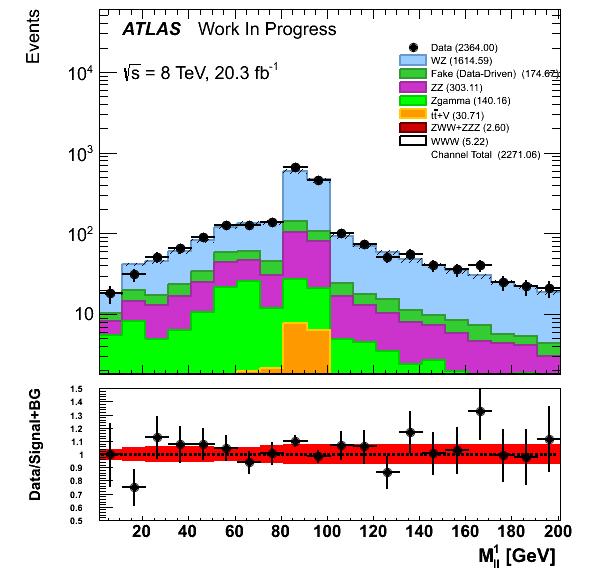
\includegraphics[width=0.4\textwidth]{figures/WZ_CR/InvariantMassSFOS_histratio.png}
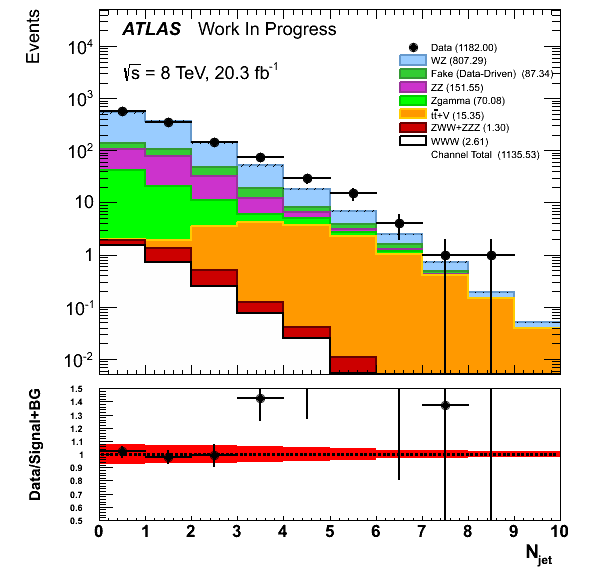
\includegraphics[width=0.4\textwidth]{figures/WZ_CR/NJets_histratio.png}
\caption{$WZ$ control region with 3 lepton pre-selection plus 2 SFOS requirement. 
Distributions show leading lepton $p_{T}$, $\MET$, $m_{12}$, and jet multiplicity. 
The systematic band shows the uncertainty on the $WZ$ k-factor.}
\label{fig:WZ_2SFOS_CR}
\end{figure}  

As a further test of the method, a MC estimate which includes the $WZ$ signal as
well as the electroweak and fake backgrounds is used as input in place 
of $N^{\textrm{Data}}_{A,B}$ to see if the MC estimate for the $WZ$
contribution in the signal region can be recovered. This is referred to as
a closure test.  The measured value for the $WZ$ normalization from the 
closure test is found to be  $495\pm39$, which is indeed consistent with the
estimate from pure MC of $498\pm1$. The closure test also shows consistent
results when varying the normalizations of the different compoenents 
in the MC independently.




\subsubsection{$ZZ\rightarrow llll$}
\label{sec:zzbg}

The $ZZ\rightarrow llll$ process has a similar cross-section as 
the $WZ\rightarrow lll\nu$ process but is 
suppressed by the probability that exactly one lepton is not reconstructed. 
Still, this probability is large enough that the $ZZ$ background is one of the 
largest in the 1 and 2 SFOS signal regions.  This background is simulated
using MC as descrbed in \sec\ref{sec:www_bg_samples}.
Unlike the $WZ$ process, NNLO predictions are available 
from~\cite{Cascioli:2014yka,Baglio:2013toa,Bierweiler:2013dja}
that suggest a k-factor of 1.05 on the overall $ZZ$ prediction.
The uncertainty on the prediction is determined to be 
15\%~\cite{Cascioli:2014yka,Baglio:2013toa,Bierweiler:2013dja}.
This correction is used instead of determining a correction in the data
like in \sec\ref{sec:wzbg}.

We may check how well the NLO $ZZ\rightarrow llll$ MC prediction and 
NNLO normalization correction describe the process in the data by looking
in a four lepton control region. The leptons are required to have
the same quality requirements as in \sec\ref{sec:object_selection}.
The leptons are sorted by \pt~with the highest \pt~lepton
required to have $\pt>25\GeV$, the next two to have
$\pt>15\GeV$, and the lowest \pt~lepton to have $\pt>10\GeV$.
From these leptons, two separate SFOS pairs are formed. If there
is any ambiguity, first an SFOS pair is formed which gives the greatest
possible di-lepton invariant mass and the remaining leptons form the other pair.
This is a similar procedure to~\cite{Aad:2014wra}. Finally, 
to suppress background contamination in the control region,
the invariant mass of both SFOS pairs are required to be near the \z-mass, 
with $60<m_{\textrm{SFOS}}<120\GeV$ for both.
The results of the comparison are summarized for a few different distributions
in \fig\ref{fig:ZZ_CR} and on the total yield in \tab\ref{tab:ZZ_CR}.
The expectation is shown to agree well with the observed data within the 
stated systematic uncertainty on the k-factor of 15\%. 


%%%%Should I say anything about this off shell business? Probably not.
%It was also checked whether or not the contribution of $ZZ^{*}$ where 
%the $Z^{*}$ boson is very offshell, $m_{Z^{*}} < 4$~GeV, while the other boson
%has a  mass $m_Z > 4$~GeV has any impact on the signal regions. This was 
%evaluted by looking at the samples with channel numbers
%$181471$ through $181479$ in Table~\ref{tab:sample_bkg_dibosons}.  
%The contribution from these samples were found to be negligible, with a 
%statistical uncertainty compatible with exaxtly 0 events in the individual 
%signal regions. As a result, these samples were not considered any further 
%and are not included in the final background  estimate for the signal regions 
%or in the ZZ control regions.


\begin{figure}[htp]
\centering
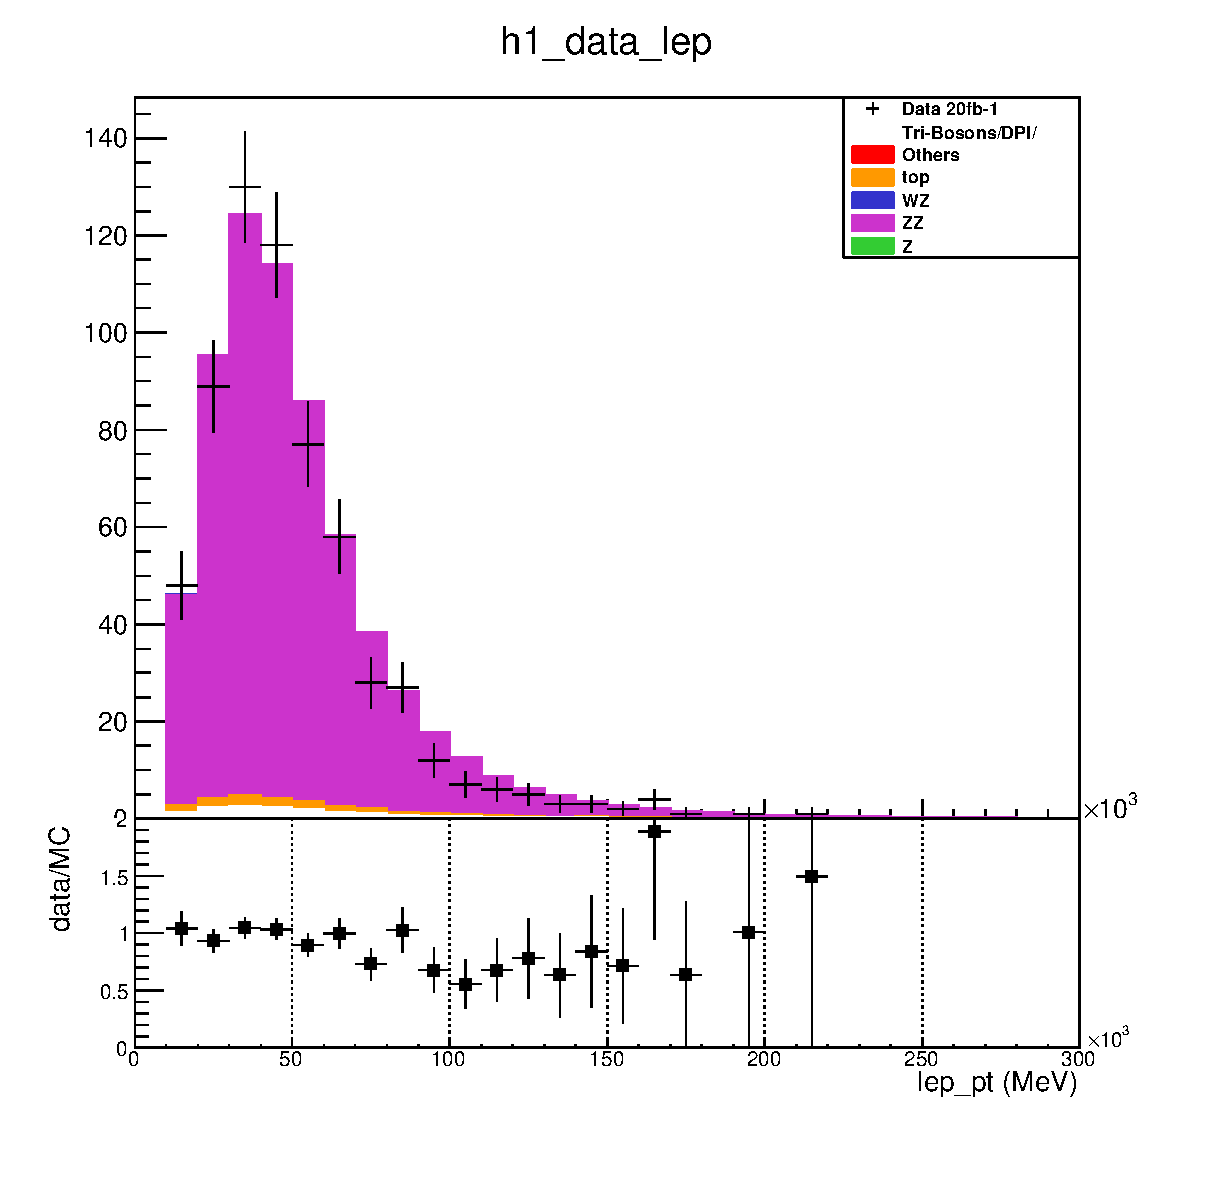
\includegraphics[width=0.4\textwidth]{figures/ZZ_CR/ZZ_CR_lep_pt.eps}
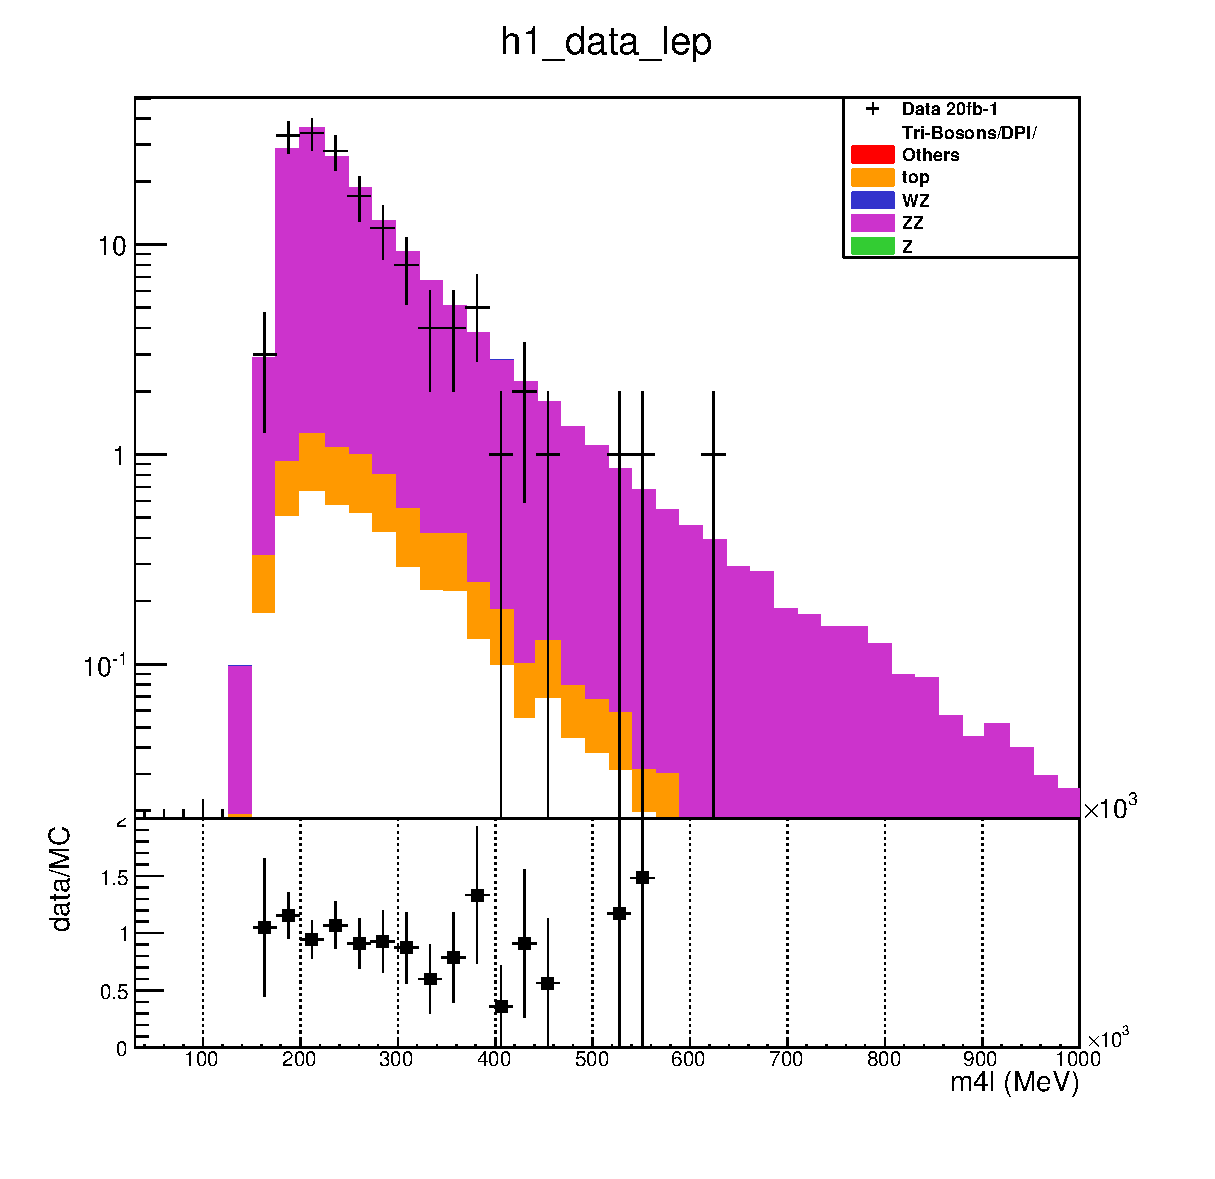
\includegraphics[width=0.4\textwidth]{figures/ZZ_CR/ZZ_CR_m4l.eps}
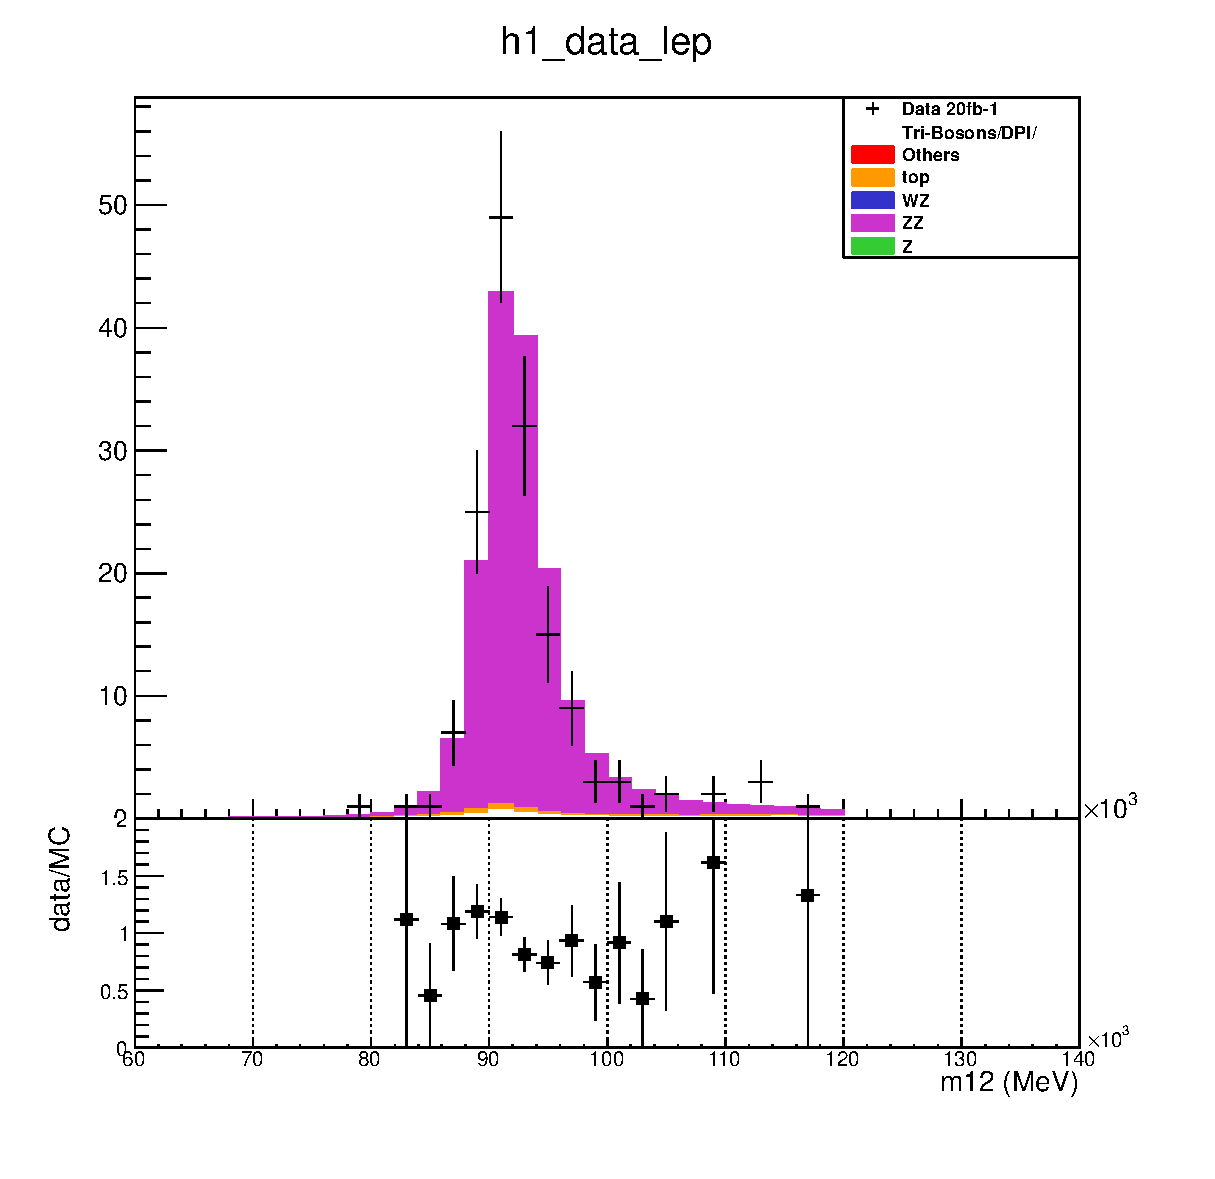
\includegraphics[width=0.4\textwidth]{figures/ZZ_CR/ZZ_CR_m12.eps}
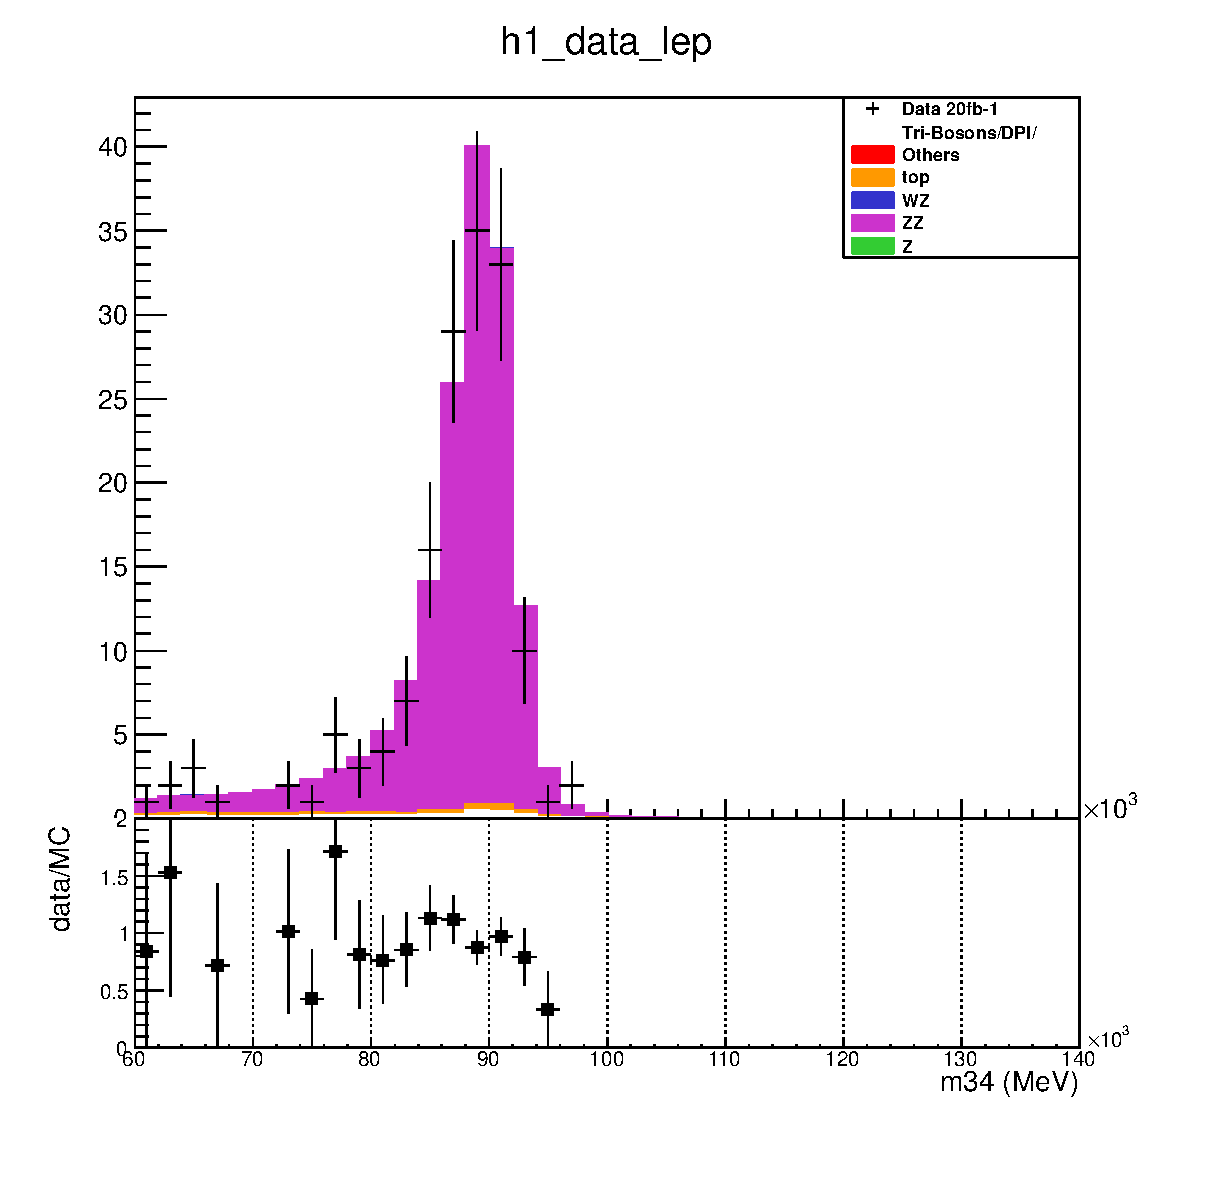
\includegraphics[width=0.4\textwidth]{figures/ZZ_CR/ZZ_CR_m34.eps}

\caption{$ZZ\rightarrow lll$ control region with two separate SFOS pairs. 
Distribution are shown for the lepton \pt, the leading di-lepton mass ($m_{12}$), 
the minimum di-lepton mass ($m_{34}$), and the four lepton mass ($m_{4l}$).}
\label{fig:ZZ_CR}
\end{figure}  

\begin{table}[htp]
\centering
\begin{tabular}{|c||c|c|c|c|}
\hline
 & Event Yield\\ 
\hline\hline
$WZ$ &  $0.05 \pm 0.01$\\ 
$ZZ$ &  $156.2 \pm 0.3$(stat) $\pm 22.3$(syst) \\ 
% $gg2ZZ$ &	$21.3 \pm 0.2$ \\
$Z\gamma$ &  $0.0 \pm 0.0$\\ 
Fake (MC) &  $3.6 \pm 0.2$\\ 
triboson and $t\bar{t}+V$ &  $4.1 \pm 0.2$\\ 
\hline
Expected Signal + Background &  $164.0 \pm 0.3$ (stat) $\pm 22.3$(syst)\\ 
\hline
Observed Data &  $155$\\ % \pm 12$\\ 
\hline
\end{tabular}
\caption{Number of data and predicted events in the $ZZ$ control region. 
The error quoted on the MC samples represents only the statistical error. 
The systematic error due to the k-factor on the $ZZ$ sample is also shown.}
\label{tab:ZZ_CR}
\end{table}


\clearpage

\subsubsection{$Z\gamma$}
\label{sec:zgammabg}

The $\z\gamma$ process can produce three leptons and thus fall into the 
signal regions as described in \sec\ref{sec:www_bg_samples}.
Measurements of this process within ATLAS
have shown that this process is well described from MC simulation
using the \sherpa~generator at both 7 and 8\TeV~\cite{Aad:2013izg,Auerbach:1631102}.
Thus, no further correction or uncertainty on the normalization is applied.

The description of the $\z\gamma$ process is tested in a three lepton control
region starting from the 
pre-selection (described in \sec\ref{sec:preselection}) and with the same
lepton quality requirements as in \sec\ref{sec:object_selection}.
One of the three leptons should be an electron while the remaining two 
are required to form a di-muon SFOS pair. For this final state to be produced
by the $\z\gamma$ process, the electron should always come from 
pair production off of the photon, $\gamma$, which itself radiates
off of the initial state \z~boson.  As a result, the invariant mass
of the di-muon pair coming from the \z-decay will typically be shifted
slightly below the \z-mass. However, the invariant mass of the three lepton 
system should restore this shift such that the mass peak is again centered 
on the \z-mass. Thus, in order to further suppress backgrounds to the 
$\z\gamma$ process, we also require that the three-lepton invariant
mass, $m_{\mu\mu e}$, be within 15\GeV of the \z-mass.
The prediction after this selection is compared to data for a few different
distributions in \fig\ref{fig:Zgamma_CR} and for the total yield
in \tab\ref{tab:Zgamma_CR}. The control region is clearly enhanced
in the $\z\gamma$ process, and furthermore shows very good agreement. 
This is even true for distributions of the electron kinematics, 
such as $\eta$ and $\pt$, which suggests that the photon conversion
mechanism is being well modelled.

\begin{figure}[htp]
\centering
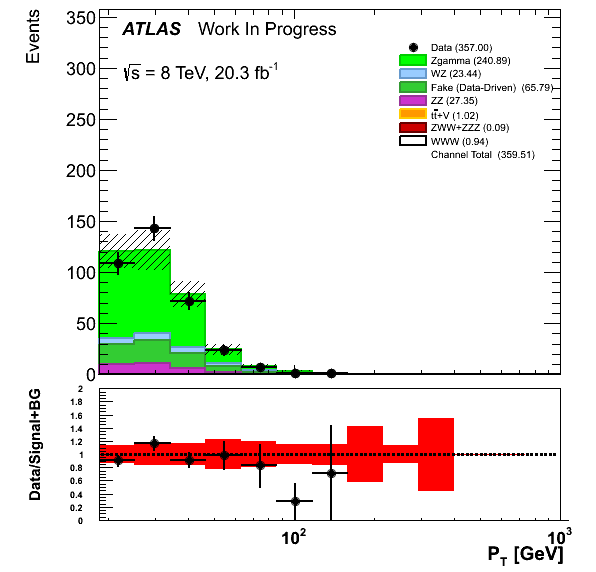
\includegraphics[width=0.4\textwidth]{figures/ZG_CR/AllLeptonPt_histratio.png}
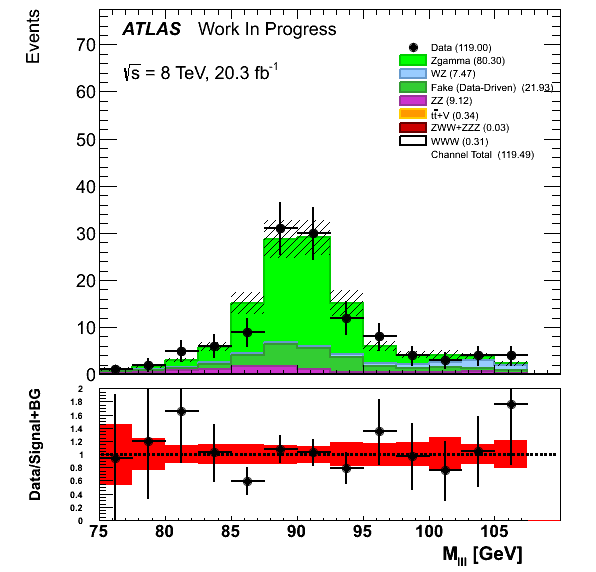
\includegraphics[width=0.4\textwidth]{figures/ZG_CR/InvariantMassThreeLep_histratio.png}
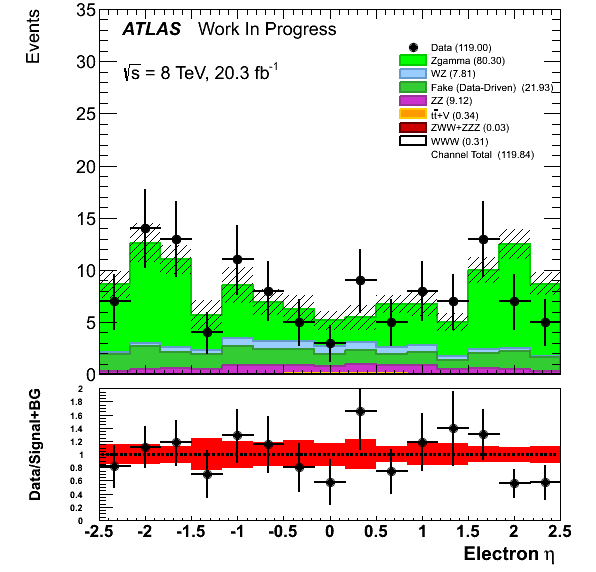
\includegraphics[width=0.4\textwidth]{figures/ZG_CR/ElectronEta_histratio.png}
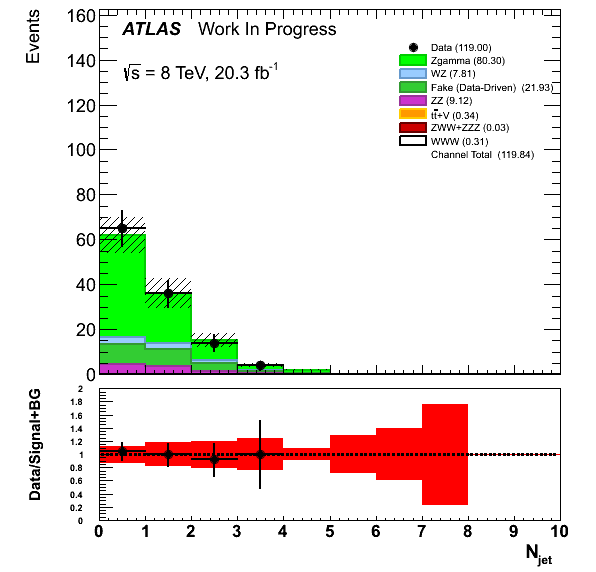
\includegraphics[width=0.4\textwidth]{figures/ZG_CR/NJets_histratio.png}

\caption{Three lepton $Z\gamma$ control cegion. Distribution are shown for the
lepton $p_{T}$, three lepton invariant mass ($m_{\mu\mu e}$), electron $\eta$, 
and jet multiplicity.}
\label{fig:Zgamma_CR}
\end{figure}  


\begin{table}[ht!]
\centering
\begin{tabular}{|c||c|c|c|c|}
\hline
 & Event Yield\\ 
\hline\hline
$WZ$ &  $7.47 \pm 0.11$\\ 
$ZZ$ &  $9.116 \pm 0.075$\\ 
$Z\gamma$ &  $80.3 \pm 2.8$\\ 
$ZWW+ZZZ$ &  $0.0285 \pm 0.0046$\\ 
$t\bar{t}+V$ &  $0.338 \pm 0.012$\\ 
Fake (data-driven) &  $21.9 \pm 1.2$\\ 
$WWW$ &  $0.3142 \pm 0.0072$\\ 
\hline
Expected Background &  $119.2 \pm 3.1$\\ 
Expected Signal + Background &  $119.5 \pm 3.1$\\ 
\hline
Observed Data &  $119 \pm 11$\\ 
\hline
\end{tabular}

\caption{Expected and observed event yields for the Z$\gamma$ control region. 
Only statistical uncertainties are shown.}
\label{tab:Zgamma_CR}
\end{table}



\subsubsection{Double parton scattering, $\ttbar + V$, and $VVV$}

\paragraph{DPS}
\label{sec:bkg_DPS}
Double parton scattering (DPS) backgrounds are also taken into account in the analysis. To estimate their contribution a list of samples used in the same sign WW analysis~\cite{Aad:2014zda,DPS:Twiki} has been used. The cross section of these processes can not be taken directly from MC, but it must be further studied. Considering the DPS production of $A+B$, where $A$ and $B$ can be products of any single-parton, the cross section can can be factorised as~\cite{Gaunt:2010pi}:
\begin{equation}
	\sigma^{DPS}_{(A+B)}=\frac{m}{2}\times{}\frac{\sigma^{S}_{A}\times{}\sigma^{S}_{B}}{\sigma_{eff}}
\end{equation}	

Where $\sigma^{S}_{(A/B)}$ is the single-parton scattering production cross-section of the process $A/B$, $m$ is a factor which takes the value of 1 when $A=B$ and 2 when $A\ne B$, $\sigma_{eff}$ is the effective cross section of the proton. A measurement of $\sigma_{eff} =15\pm3(stat)^{+5}_{-3}(syst)$ mb for 7~\TeV{} $p-p$ collisions has been recently performed by ATLAS~\cite{Aad:2013bjm}. By factorizing the cross-section in this form, the correlation between the two parton interactions are neglected.

The samples and cross section that have been used in this analysis are given in Table~\ref{tab:sample_bkg_dibosons_gg2DPI}. An uncertainty of $50\%$ is applied on the normalization of these processes. Among these processes the one that can give a tri-lepton final state are: $WZ$, $ZZ$, and $Z\gamma$.
	
Their contributions are found to be negligible.


\paragraph{Other backgrounds}
The other backgrounds evaluated from MC are the one containing three real leptons: $t\bar{t}+V$, $WWZ$, and $WZZ$.
The PDF and scale uncertainties for the $t\bar{t}+V$ processes have been evaluated by other member of the ATLAS collaboration~\cite{ttV:Twiki}, and found
to be about $30\%$ of their normalization. These processes have been recently measured by the ATLAS collaboration~\cite{ATLAS-CONF-2015-032}, and their normalization are found to be consistent with the NLO predictions.

An equivalent $30\%$ uncertainty is assigned for the other $VVV$ contributions ($ZWW^{*}$ and $ZZZ^{*}$) that are not coming from our signal.

% Other background contributions are arising from tt¯+V, t+V and VVV processes. They will be estimated
%  using MC samples and global normalization uncertainties are associated to these MC predictions. An
%  uncertainty of 30\% is assigned to the tt¯+ V contribution, according to [27]. An uncertainty of 30\% is
%  also assigned to the VVV contribution.

%
%include diagram

\unitlength = 0.8mm %necessary for feynmp
\begin{figure}[ht]
\centering
\vspace{5 mm}
\begin{fmffile}{feynchargemisid}
		\begin{fmfgraph*}(80,50)
			\fmfleft{i1}
			\fmfright{o1,o2,o3}
			\fmf{fermion}{i1,v1}
			\fmf{fermion}{v1,o3}
			\fmf{photon,label=$\gamma$}{v1,v2}
			\fmf{fermion}{o1,v2}
			\fmf{fermion}{v2,o2}
			\fmflabel{$e^-$}{i1}
			\fmflabel{$e^+$}{o1}
			\fmflabel{$e^-$}{o2}
			\fmflabel{$e^-$}{o3}
			%\fmflabel{$W^+$}{i1}
			%\fmflabel{$e_L,\mu_L,\tau_L$}{o1}
			%\fmflabel{$\overline{\nu}_{e,R},\overline{\nu}_{\mu,R},\overline{\nu}_{\tau,R}$}{o2}
			%\fmflabel{$e_L$}{o1}
			%\fmflabel{$\overline{\nu}_{e,R}$}{o2}
		\end{fmfgraph*}
\end{fmffile}
\vspace{2 mm}
\caption{Feynman diagram showing combination of bremsstrahlung and pair-production 
processes that lead to electron charge mis-identification. In this case, 
we start with an electron and end with two electrons and a positron. For
electron charge mis-identification to occur, the positron would have to 
be the only final state particle that is reconstructed.}
\label{fig:feyn_chargemisid}
\end{figure}


High energy electrons
produced from the 
hard scatter of the proton-proton
collisions of the LHC
will frequently radiate photons in the presence of the ATLAS
detector material via bremsstrahlung. 
Furthermore, it is also common %how common?
for high energy photons to convert into electron-positron pairs.
Chaining these two processes together will cause 
an electron to radiate a photon which then produces an
electron-positron pair, resulting in a three body final state with
two electrons and a positron, such as in the Feynman diagram
of \fig\ref{fig:feyn_chargemisid}.
For muons, their larger mass suppresses these phenomena
such that the similar effect for muons is completely negligible.

Often, the energy difference between the products in the final state will
be large, such that most of the energy is carried away in only one
product.  It is thus possible that a majority of the energy of the initial
electron is carried away in the positron, which
has an opposite charge.  If the energy imbalance is large enough,
the other two final state electrons may not have enough
energy to be reconstructed. As a result, the initial electron
will instead be measured as a positron, and the 
charge of the initial state electron will have effectively 
been mis-identified. The situation is reversed if starting
with a positron.  Throughout the rest of this  section we use 
electrons to collectively refer to both electrons and positrons
unless otherwise specified.



The strong dependence of charge mis-identification 
upon the ATLAS material means that care must be
taken when describing this process. In particular, the material 
description in MC, while sophisticated, is not perfect. 
Thus, it would be better to use the data itself to determine
a model for these rates where it does not rely on a model of the detector.
Thus, we extract the rates of electron charge 
mis-identification using the data and only use the rates determined
in MC as a cross-check.




The background due to electron charge mis-identification is most important 
for this analysis
in the 0 SFOS signal region, described in \sec\ref{sec:signal_regions},
where it is one of the only mechanisms by which the $WZ$ and $ZZ$ 
processes enter this region\footnote{The $WZ$ and $ZZ$ processes
can also enter in the 0 SFOS region if the $Z$ bosons
decay to $\tau$ leptons which then subsequently decay into 
either electrons or muons with the proper charge and flavor combination.
See \sec\ref{sec:chargemisid_validation}}.
Without electron charge mis-identification, these events would fall
equally in the 1 and 2 SFOS regions.
As will be seen shortly, the overall rate of electron charge mis-identification
is quite small. 
Furthermore, it will be seen that the total background in the 0 SFOS region is 
a good deal smaller than the 1 and 2 SFOS regions. Thus, the
migration of events from the 1 and 2 SFOS regions to the 0 SFOS 
region, resulting from electron charge mis-identification, has
a larger relative impact on the background in the 0 SFOS 
region\footnote{There is also a migration from the 0 SFOS to the 1 and 2 SFOS 
regions, but the relative number of 0 SFOS events to 1 and 2 SFOS
events before electron mis-identification is so small as to make this
effect completely negligible.}.
As a result, we focus only on modeling the background due to electron
charge mis-identification in the 0 SFOS region and assume that an 
out of the box estimate of this background from MC is adequate for the 
1 and 2 SFOS regions.


The electron charge mis-identification background is determined
for the 0 SFOS signal region by first extracting the electron charge
mis-identification rates using the data as a model,
described below. The extracted
rates are compared to an alternative method using only MC. 
The difference between the two is used as a systematic on the
rates. The rates are then used to re-weight the $WZ$ and $ZZ$ MC samples
on an event-by-event basis 
according to the probability that electron charge mis-identification
could cause the event to migrate into the 0 SFOS region. In this way, 
the full statistics of the MC samples can be utilized to get a model of
the behavior of these processes in the 0 SFOS region, while also taking 
into account a more accurate material description. Other backgrounds
due to electron charge mis-identification are assumed to be negligible.
More details on the methods used to extract the rates and the re-weighting
method are provided below.




\subsubsection{Charge Mis-identification Rate Extraction}
\label{sec:chargemisd_rates}

The rate of electron charge mis-identification is defined as 
the probability that an electron has its charge mis-identified.
These rates depend highly on the kinematics of the individual electrons.
In particular, the sensitivity to material dependence described above 
means that the rate depends on where in the detector the electrons
pass through. In general, the material density of the ATLAS
detector increases for high \eta~(i.e. as the electron gets closer to the
beam pipe), as seen in \sec\ref{sec:atlas_id}. The rate also increases as a function of the electron energy, 
or \pt. These are the two most important kinematic variables for determining
the rate\footnote{The material also varies as a function of the azimuthal angle,
$\phi$, in the detector. However, this is a sub-dominant effect. Furthermore,
increasing the dimensionality further significantly harms the statistical 
power of the method. Thus it is ignored.}, and 
so the rate extraction is binned as a function of both with nine $\eta$ 
bins ranging from 0 to 2.5 and six \pt~bins ranging from 15 to 120 \GeV~plus
an additional overflow bin for $\pt>120\GeV$.



The rates are studied in a region with two electrons passing the object
selection from \sec\ref{sec:object_selection} and that have
a di-lepton mass within 10~\GeV~of the \z~mass. No requirements are placed
on their charge. Two different methods
are used: one using purely MC and one using the data.
The method using MC takes $\z\rightarrow ee$ MC simulation 
and relies on being able to determine the charge of each electron from the 
\z~decay by looking 
directly at the hard scattering process as provided by the generator.
This is called ``truth'' information, at which point the processes of radiation
and pair-production have not occurred. It then compares
these truth electrons to the ``reconstructed'' electrons 
measured after all processes, including those of radiation and pair-production,
have been simulated and reconstructed
in the detector. The truth and reconstructed electrons
are matched by asking that they are nearby each other in $\eta$ and $\phi$.
The charge of the matched truth and reconstruction electrons 
are then compared to see if 
the charges agree
and tallying  this 
for the appropriate $\pt$ and $\eta$ bin. Once all MC events
have been recorded, the rate per bin may be determined simply 
by taking the ratio of the number of electrons where the truth and reconstructed
electron charge disagreed per bin to the total number of electrons per bin. 

The method using the data instead is the nominal method used 
for extracting the electron charge mis-identification
rates.
It uses the same selection as in the MC method, with the events
categorized based on whether the electrons from the \z~decay 
are of the same-sign or of opposite-sign.
However, in this case
there is no truth information to tell which electron's charge
has been mis-identified. Instead, we assume that those events in
the same-sign category are due purely to charge mis-identification
and attempt to extract the rates by minimizing a likelihood.
Refer to the rate for an electron in a 
particular $\pt$ and $\eta$ bin $i$ as $\varepsilon_i$.
Also, refer to the total number of di-electron events observed in data with one electron
in bin $i$ and the other in bin $j$ as $N_{i,j}$.
Given the rates, the expected number of same-sign events
should be approximately $N_{i,j}(\varepsilon_i + \varepsilon_j)$,
where we have ignored higher order terms, which account for  
the probability for both electrons to have their
charges flipped, since they should be small. We do
not know the rates \emph{a priori}, but they should follow 
a Poisson likelihood given the observed total number of events,
$N_{i,j}$, and the the observed number of same sign events,
$N_{i,j}^{\textrm{SS}}$, with the following form:
\begin{equation}
\curlyl( \varepsilon_i,\varepsilon_j | N_{i,j}^{\textrm{SS}},N_{i,j})
=
\frac{(N_{i,j}(\varepsilon_i+\varepsilon_j))^{N^{\textrm{SS}}_{i,j}} e^{-N_{i,j}(\varepsilon_i+\varepsilon_j)}}{N^{\textrm{SS}}_{i,j}!}
\end{equation}
From this, we may construct a log likelihood which can be minimized
as a function of $\varepsilon_i$ and $\varepsilon_j$:
\begin{equation}
-\ln \curlyl( \varepsilon_i,\varepsilon_j | N_{i,j}^{\textrm{SS}},N_{i,j}) = 
N_{i,j}(\varepsilon_i+\varepsilon_j)
- N^{\textrm{SS}}_{i,j} \ln(N_{i,j}(\varepsilon_i+\varepsilon_j))
\end{equation}
where the terms that are not dependent on $\varepsilon_i$
and $\varepsilon_j$ have been dropped.
Thus, given the data, the values of $\varepsilon_i$ and $\varepsilon_j$
at the minimum value of the log likelihood are taken as the estimate
of the rates.
Backgrounds to the $Z\rightarrow ee$ process are subtracted using MC.

\begin{figure}[htp]
\centering
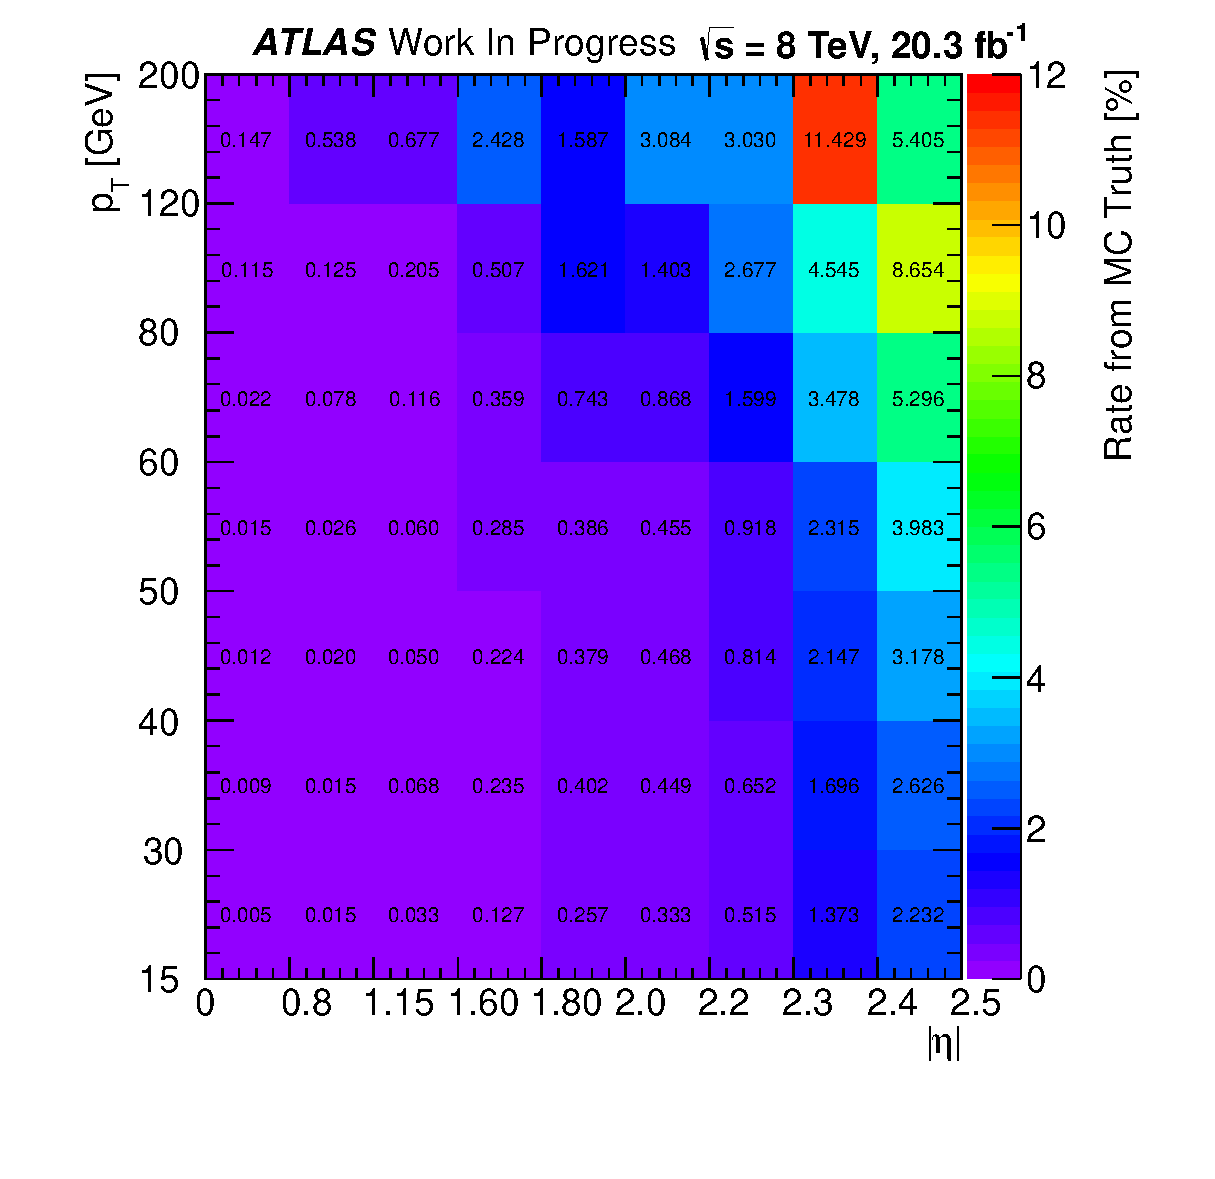
\includegraphics[width=0.45\columnwidth]{figures/ChargeMisID/Nov5_2015_TruthRates_Plot.eps}
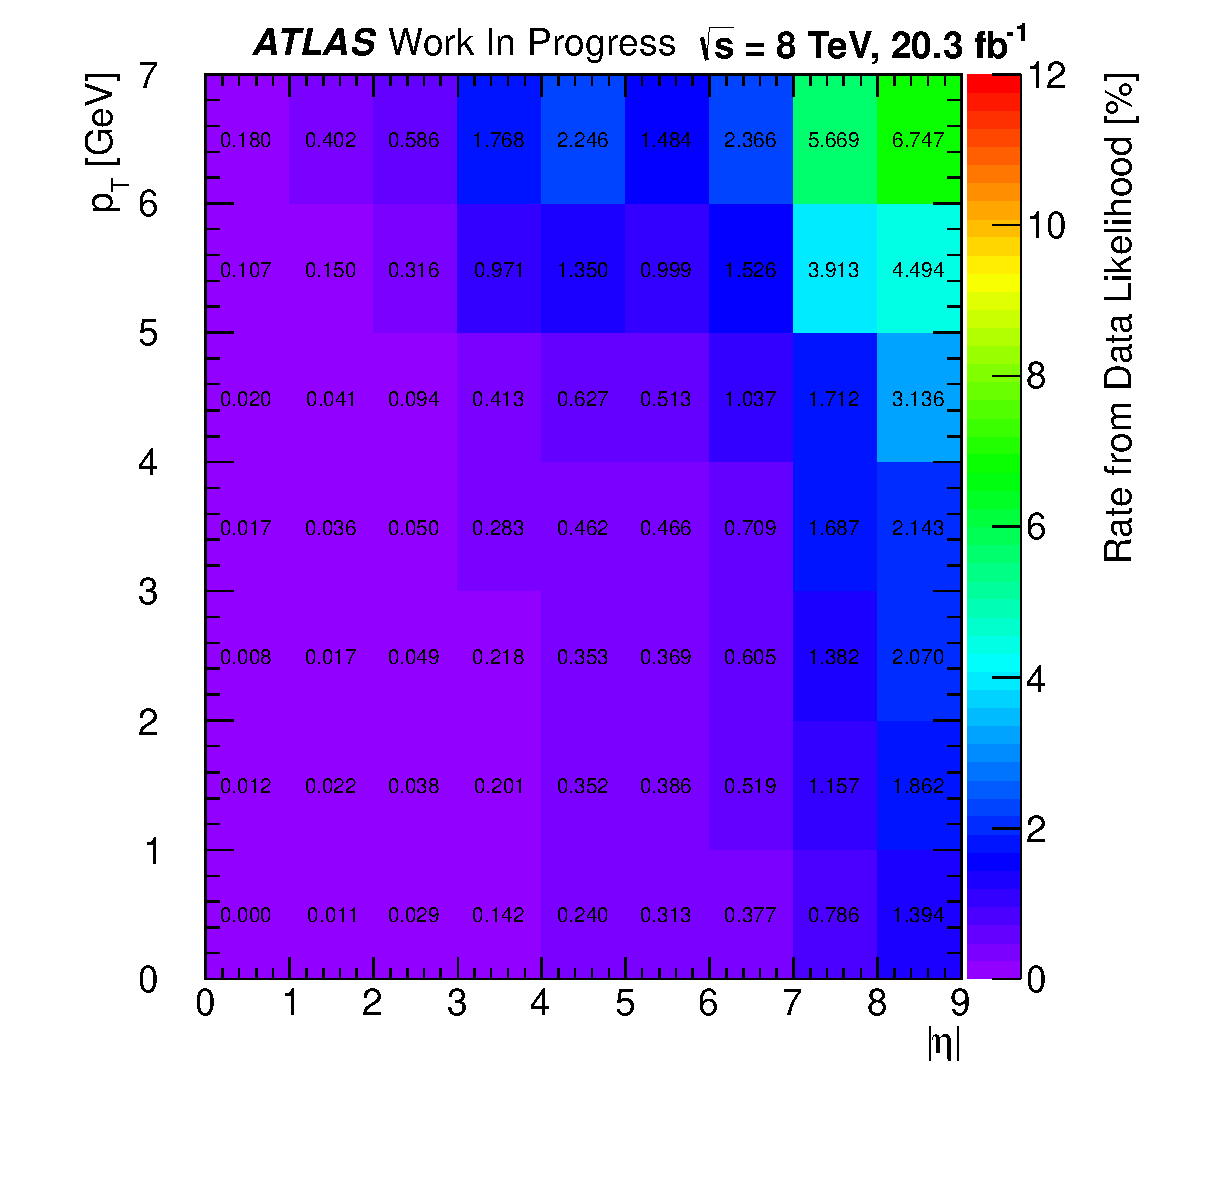
\includegraphics[width=0.45\columnwidth]{figures/ChargeMisID/Nov5_2015_DataRates_Plot.eps}
\caption{Electron charge mis-identification rates as a function of
the electron \pt and $\eta$ extracted using the MC
truth method (left) and the likelihood method in data (right). }
\label{fig:chargemisid_rates_contour}
\end{figure}

The rates for the two different methods are 
shown in \fig\ref{fig:chargemisid_rates_contour}.
For low values of \pt~and $\eta$, where most electrons fall, 
the rate is small enough to be negligible. 
The rate increases gradually along both dimensions, reaching as much as
6.7\% in the region $\pt > 120\GeV$ and $2.4 < |\eta| < 2.5$ as measured
in the data, which corresponds to the highest bin in both dimensions. 
Still, the average rate is only around 0.01 \% to 0.1 \%.
The rates measured using MC truth information are systematically higher
than those measured in data, almost by a factor of two, discussed later.
%figure 4.45 in jinst?
%or maybe https://atlas.web.cern.ch/Atlas/GROUPS/PHYSICS/PAPERS/PERF-2013-05/
%or https://atlas.web.cern.ch/Atlas/GROUPS/PHYSICS/PAPERS/PERF-2013-03/
%might it be that the material description was improved in a later version of the MC?
%mc12b is known to have a maybe 20-30% lower rate of photon conversions overall
%according to Jake, I guess because of the material description.
%could the improved simulation referred to in one of the papers above
%be for something that was included after mc12b? probably
%ruiqi used this sample for the MC generation:
%mc12 8TeV.147806.Powheg Pythia8 AU2CT10 Zee.merge.NTUP COMMON.e1169 s1469 s1470 r3542 r3549 p1562
%this twiki
%https://twiki.cern.ch/twiki/bin/view/Atlas/MC12cWiki?rev=3
%claims that improvements to the geometry came in mc12c
%However, these improvements claim that the improved geometry
%describes more material at high eta. It seems like this would only 
%make the disagreement between the mc and data rates, assuming
%that more material really does cause more conversion
%the paper claims the difference is in part to an incomplete
%description of SCT cooling pipes.
%the most discrepant region is between eta of 1.4 and 1.6, where the 
%difference would be consistent if material were removed.
%but this then would seem to suggest that the differences show up mostly
%in eta bin 3, which they do not. Instead it grows starting
%for eta > 2.0




%note: the material description shouldn't be affecting our zgamma
%estimate since it requires a b-layer hit so these are converting early

Some variations on the method are also performed
in order to better assess its performance 
and to determine systematic uncertainties.
One variation is to perform the same likelihood extraction
as in the data, but using only reconstructed MC. This produces
similar rates to the truth MC method, suggesting that the differences
seen between the data likelihood method and the truth MC method
are not due to the method itself. 
Another variation is to extract the rates from the data with the 
likelihood method but without performing the background
subtraction. 
%In the original method, the background subtraction is performed by...  ...with a template fit like in \fig\ref{fig:chargemisid_fitexample}.  
%\begin{figure}[htp]
%\centering
%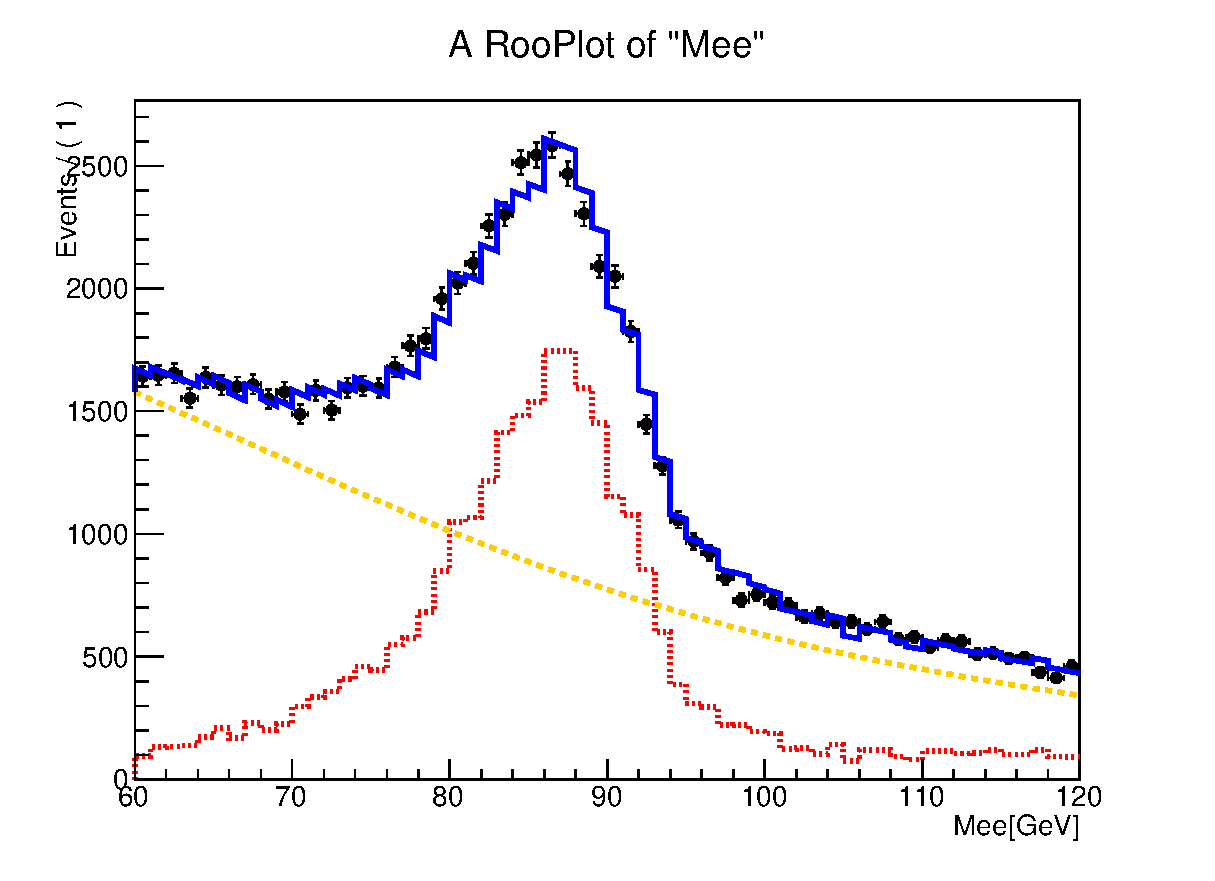
\includegraphics[width=0.6\textwidth]{figures/ChargeMisID/Tot_Polynomial_0_2.eps}
%\caption{Plot of the di-lepton invariant mass 
%in the region where one electron has $0 < |\eta_1| < 0.8$
%and the other has $1.15 < |\eta_2|<1.6$. The data (black points)
%are shown in a region where the electron isolation cuts are removed
%and the electron quality requirements are loosened.
%A template from $Z\rightarrow ee$ MC (red line) and a polynomial
%curve (orange line) are used to fit the data. The sum of the fit
%(blue line) is seen to fit the data well.}
%\label{fig:chargemisid_fitexample}
%\end{figure} 


The different variations on  rate estimation are compared to the 
nominal estimate to extract
a final systematic. In \fig\ref{fig:ChargeMisID_truthRate_finalFig},
the two-dimensional rates are unfolded into one-dimension
with the bins numbered counting from low values of $\eta$ and \pt~to
high values. The rates with and without background
subtraction are seen to agree quite well, only 
differing by about 5-6\% throughout.  
The red curve shows the rates evaluated using the same likelihood method
applied to the data, but using only reconstructed MC. 
This variation on the likelihood method using just MC
is seen to follow the MC truth method closely, except in a few bins where the statistics
are low. The relative difference between the MC truth and MC likelihood methods
is transported to the nominal estimate in data and used as another systematic.
There is a factor of two difference in the rates evaluated using MC
and those using data, with the difference persisting regardless of the methods used. 
This suggests that the difference is coming from the MC itself, motivating the
use of the data-driven rate evaluation in the first place. 
As such, the difference between the methods using data and those using MC is not
used as a systematic.
The systematic uncertainties are combined in quadrature with the statistical
uncertainty on the nominal estimate to arrive at a final uncertainty on the
rates, shown as a hashed band.


\begin{figure}[htp]
\centering
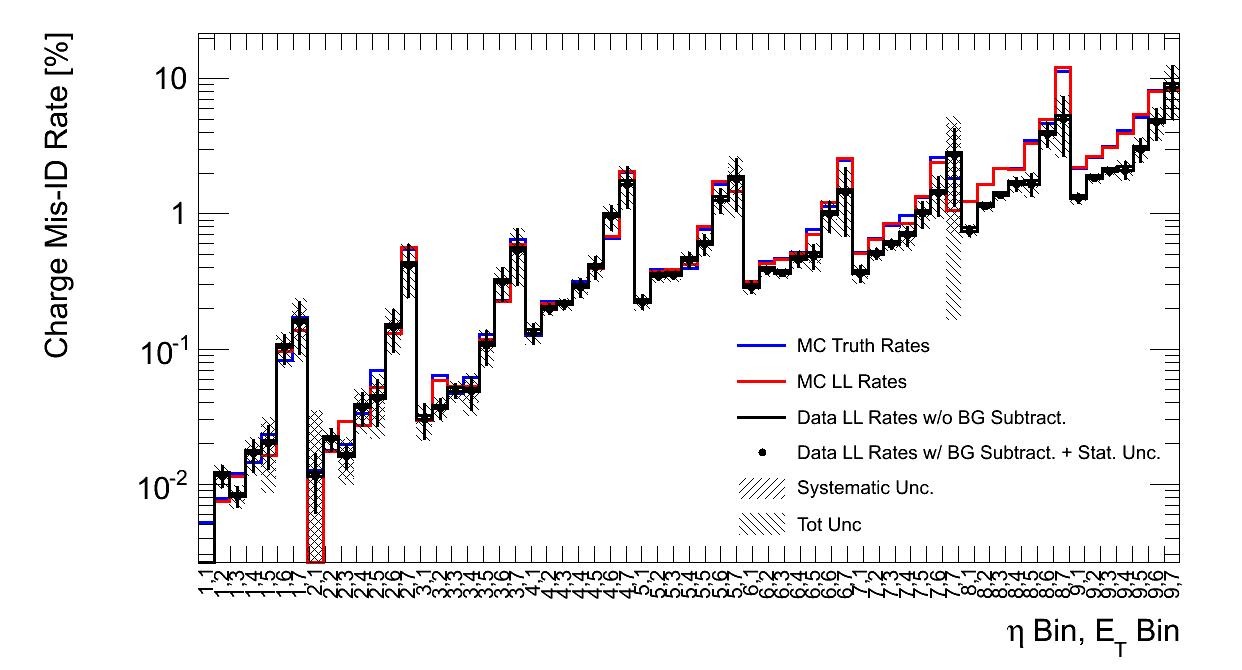
\includegraphics[width=0.9\textwidth]{figures/ChargeMisID/Validation_ChargeMisIDRates_PTvsEta_FinalRateWithSys.png}
\caption{Summary of electron charge mis-identification rates using
the likelihood method in data with background subtraction (black points) 
and without background subtraction (black line), the MC truth 
method (blue line), and the likelihood method in MC (red).
Systematic uncertainties are extracted as described in the text and are shown
in the gray hashed band pointing from bottom left to top right. 
The systematic uncertainties are combined with the statistical uncertainties
on the black points to arrive at a total uncertainty on the rates, shown 
in the hashed band pointing from bottom right to top left.}
\label{fig:ChargeMisID_truthRate_finalFig}
\end{figure}




\subsubsection{Di-boson MC Re-weighting}


The electron charge mis-identification  rates are primarily important for the determination of the $WZ$ and $ZZ$ background contamination in the 0 SFOS region,
as mentioned already.
Once derived, the rates are applied to $WZ$ and $ZZ$ MC samples based on 
whether or not a charge flip could cause the event to appear in the 0 SFOS region.  
In particular, the following di-boson decays are considered:
\begin{itemize}
\item $WZ\rightarrow e^{\pm}\nu~ e^{+}e^{-}$
\item $WZ\rightarrow \mu^{\pm}\nu~ e^{+}e^{-}$
\item $WZ\rightarrow \tau^{\pm}\nu~ e^{+}e^{-}$
\item $ZZ\rightarrow e^{+}e^{-}~e^{+}e^{-}$
\item $ZZ\rightarrow \mu^{+}\mu^{-}~ e^{+}e^{-}$
\end{itemize}
No other decay channels are considered.  These all share in common that they 
have at least one electron-positron pair.  
Except for the $WZ\rightarrow \tau^{\pm}\nu~e^{+}e^{-}$ decay channel, 
decay channels with tau leptons are not considered
because they are suppressed by the tau branching fraction and are 
thus negligible.

The charge mis-identification rates are then applied to these channels on an 
event-by-event basis as follows.
For each event that is processed, its decay channel is identified 
at truth level. Each reconstructed lepton
is examined  and assigned a rate, i.e. a probability to charge flip, 
based on its reconstructed $\pt$ and $\eta$ values.
The probability for a charge flip to occur in an event is then approximately 
the sum of rates for the individual electrons:
\begin{equation}
p(\textrm{Charge Mis-Identification in Event}) \approx \sum_{i \in \textrm{Electrons}}  \textrm{Rate}(\pt^i,\eta^i) 
\end{equation}
Higher order terms where multiple electrons are charge mis-identified is negligible.
We are only concerned with the probability that a charge flip results in the 
event falling into the 0 SFOS region. 
Consider a step function, $\Theta(e)$, defined for an individual event:
\[
\Theta(e) = 
\begin{cases}
\hfill 1 \hfill & \text{if flipping charge of $e$ classifies event as 0 SFOS} \\
\hfill 0 \hfill & \text{if flipping charge of $e$ does NOT classify event as 0 SFOS}\\
\end{cases}
\]
Then the probability that a charge mis-identification occurs and results in 
the event falling in the 0 SFOS region is:
\begin{equation}
p(\textrm{Event is classified as 0 SFOS}) \approx \sum_{i \in \textrm{Electrons}}  \textrm{Rate}(\pt^i,\eta^i)\Theta(i) 
\end{equation}
Again, we ignore the case where multiple electrons have their charge 
mis-identified.  This probability is then used as an event-by-event weight. 


Once the weight has been determined, we then artificially flip the charge of 
one of the electrons/positrons in the event.
If there is only one electron in the event that will lead the event 
to fall in the 0 SFOS region, its charge is flipped
and one proceeds to the next event.  However, if there are multiple electrons 
in the event, there is an ambiguity that must be resolved
about which electron's charge should be flipped. One must then be careful in 
this case to not introduce any bias.
We decided to choose a procedure where we pick a single electron from the 
event at random based on the charge flip rates
of the individual electrons. Thus, for an individual electron in an 
event, the probability that it is chosen to have its charge
flipped is:
\begin{equation}
p(\textrm{$e$ has been charge flipped}) = \textrm{Rate}(\pt^e,\eta^e)\Theta(e)~/\sum_{i \in \textrm{Electrons}} \textrm{Rate}(\pt^i,\eta^i)\Theta(i)
\end{equation}

Consider an example where the event under consideration comes from the 
decay $WZ\rightarrow e^{+}\nu e^{+}e^{-}$. Assume all three charged leptons 
pass reconstruction and are selected then label 
them as: $e^{+}_1~e^{+}_2e^{-}_3$. In this case,
the only way that this event could be classified as 0 SFOS when 
flipping the charge of only one electron/positron is to flip the 
charge of the electron.
Thus, $\Theta(e^{+}_1)=\Theta(e^{+}_2)=0$ and $\Theta(e^{-}_3)=1$.  The event 
weight will then be equal to the rate of charge mis-identification 
for  $e^{-}_3$ and it will have it's charge flipped 
to be positive\footnote{This results in a final state
which does not fall into our signal region, since the sum of the
charge of the three electrons is +3. Thus, it is just for illustration purposes}.

Now consider an example of an event with 
the decay of $ZZ\rightarrow \mu^{+}\mu^{-}~ e^{+}e^{-}$.
If all four leptons are reconstructed and selected, the event will not 
be considered at all in the three lepton selection of this analysis, so 
consider the case where the $\mu^{+}$ is not selected leaving three leptons 
labeled as: $\mu^{-}_1 e^{+}_2 e^{-}_3$.  The probability for the muon to 
charge flip is negligible which leaves the electron and the positron. Flipping 
the charge of either one at a time will result in the event being 
classified as 0 SFOS.  Thus, in
this case $\Theta(\mu^{-}_1)=0$ and $\Theta(e^{+}_2)=\Theta(e^{-}_3)=1$. The 
event weight will then be the sum of the rates for $e^{+}_2$ and $e^{-}_3$.
The probability that the electron has its charge flipped is then 
$\frac{\textrm{Rate}(e^{-}_3) }{ \textrm{Rate}(e^{+}_2)+ \textrm{Rate}(e^{-}_3)}$ 
and similarly for the positron.

\subsubsection{Validation}
\label{sec:chargemisid_validation}
This procedure has been validated on the $WZ$ and $ZZ$ samples by comparing 
the predictions taken directly from MC to the predictions re-weighted in the 
0 SFOS signal region using the procedure just described. This is done in 
\fig\ref{fig:ChargeMisID_Validation_WZ} for the $WZ$ samples and on 
\fig\ref{fig:ChargeMisID_Validation_ZZ} for the $ZZ$ samples. It can be seen 
the agreement in the shape looks good for all the distributions. An offset 
between the two distributions is observed. This difference is covered partially by 
the systematic uncertainties of the method.  Any remaining difference could 
be expected from the difference in rates observed at high $\eta$ and 
high $E_{T}$ as seen in \fig\ref{fig:ChargeMisID_truthRate_finalFig} and 
serves as justification for using the data-driven method.


\begin{figure}[ht]
\centering
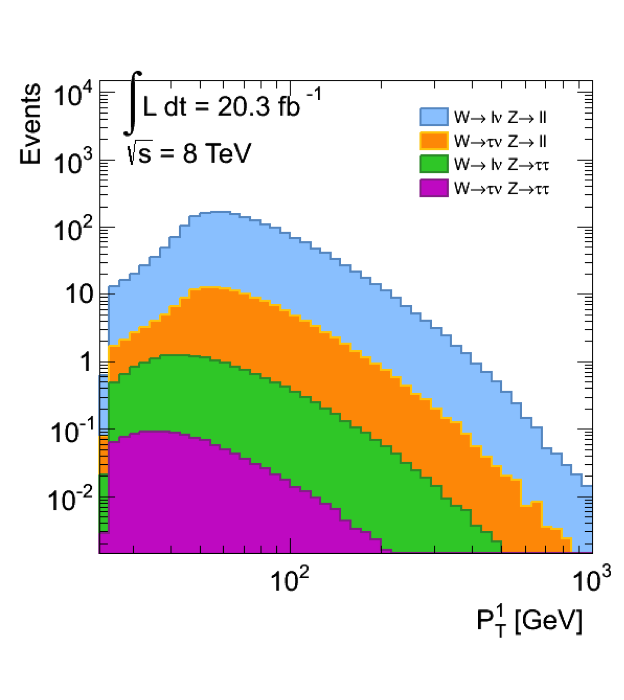
\includegraphics[width=.45\textwidth]{figures/ChargeMisID/preselection_wz_br.png}
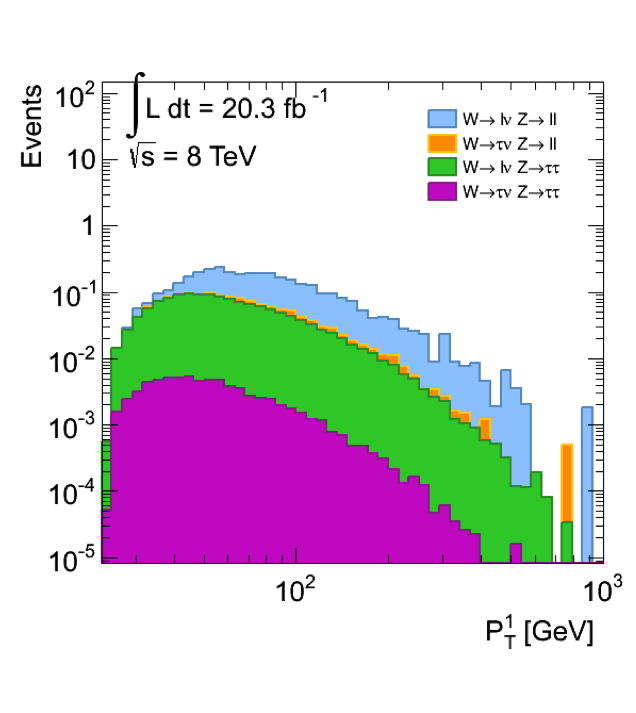
\includegraphics[width=.45\textwidth]{figures/ChargeMisID/0sfos_wz_br.png}
\caption{Plots of the different branching fractions of the $WZ$ process
as a function of the leading lepton \pt~at pre-selection (left)
and after also applying a requirement that events have 0 SFOS lepton
pairs (right). The individual decays of $W$ and $Z$ are split up
into whether they decay into taus ($\tau$) or into electrons and muons (denoted $l$).
The taus also subsequently decay. The contributions from $WZ\to l\nu ll$ 
and $WZ \to \tau \nu  ll$ after applying the 0 SFOS selection
are due purely to charge mis-identification.}
\label{fig:chargemisid_wz_br}
\end{figure}

The proportion of contributions to the $WZ$ background coming from 
charge mis-identification in the 0 SFOS region is demonstrated in 
\fig\ref{fig:chargemisid_wz_br}. Here we can see that the 
large contribution from $WZ$ decaying to electrons and muons (but not taus)
at pre-selection (see \sec\ref{sec:preselection})
survives and is non-negligible, even after applying the 0 SFOS cut.
This can only come from the electron charge being mis-identified.
It is worth noting, however, that there is also a sizable
contribution to the 0 SFOS region when the $Z$ decays to taus
since it is possible to have two leptonically decaying taus that satisfy
the 0 SFOS requirements while correctly identifying the charge.
A similar behavior occurs also for the $ZZ$ contribution.


There is no special treatment of the charge mis-identification contribution to 
other background contributions in the 0 SFOS region or to any contributions to the 
1 and 2 SFOS signal regions, including di-boson processes, as the effect is 
expected to be very small.  Any charge mis-identification events are thus 
taken directly from MC in this case.


 \begin{figure}[htp]
 \centering
 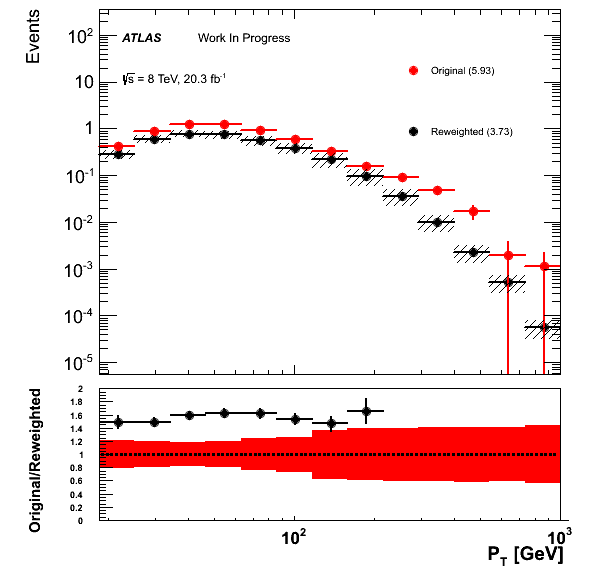
\includegraphics[width=0.4\textwidth]{figures/ChargeMisID/Validation_ChargeMisIDRates_WZ_PTLepton.png}
 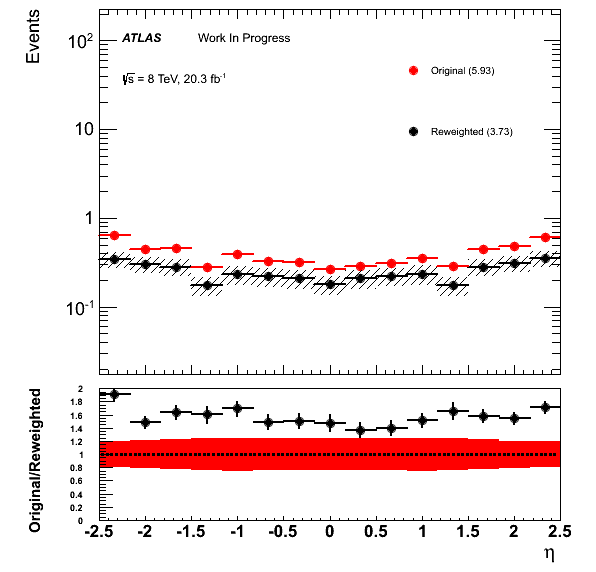
\includegraphics[width=0.4\textwidth]{figures/ChargeMisID/Validation_ChargeMisIDRates_WZ_EtaLepton.png}
 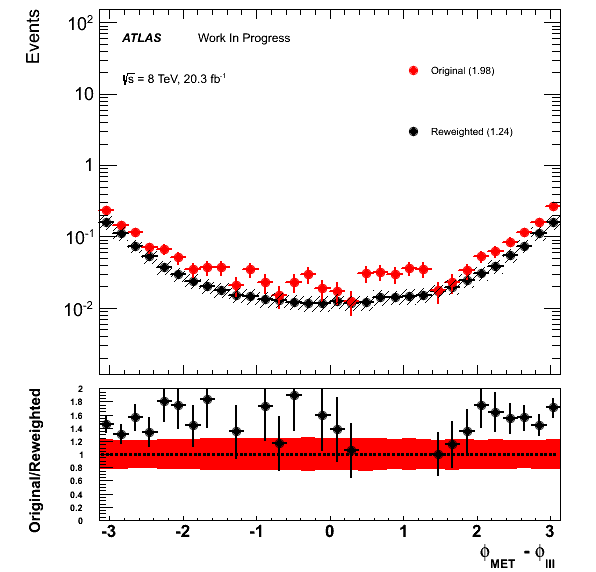
\includegraphics[width=0.4\textwidth]{figures/ChargeMisID/Validation_ChargeMisIDRates_WZ_DeltaPhi.png}
 \includegraphics[width=0.4\textwidth]{figures/ChargeMisID/Validation_ChargeMisIDRates_WZ_MET.png}
 \includegraphics[width=0.4\textwidth]{figures/ChargeMisID/Validation_ChargeMisIDRates_WZ_Mee.png}
 \includegraphics[width=0.4\textwidth]{figures/ChargeMisID/Validation_ChargeMisIDRates_WZ_JetMultiplicity.png}

 \caption{Validation of the charge mis-ID rates comparing 
 MC $WZ\rightarrow \ell ee$ ($\ell=e,\mu$) samples re-weighted with the 
 charge mis-ID rates measured in the MC $Z\to{}ee$ 
 sample to the original MC predictions. Distribution of 
 lepton $p_{T}$, $\eta$, $\Delta \phi(3l,E_{T}^{Miss})$,\met{}, Same-sign 
 di-electron invariant mass, and jet multiplicity.}
 \label{fig:ChargeMisID_Validation_WZ}
 \end{figure}
 
 
 \begin{figure}[htp]
 \centering
 \includegraphics[width=0.4\textwidth]{figures/ChargeMisID/Validation_ChargeMisIDRates_ZZ_PTLepton.png}
 \includegraphics[width=0.4\textwidth]{figures/ChargeMisID/Validation_ChargeMisIDRates_ZZ_EtaLepton.png}
 \includegraphics[width=0.4\textwidth]{figures/ChargeMisID/Validation_ChargeMisIDRates_ZZ_DeltaPhi.png}
 \includegraphics[width=0.4\textwidth]{figures/ChargeMisID/Validation_ChargeMisIDRates_ZZ_MET.png}
 \includegraphics[width=0.4\textwidth]{figures/ChargeMisID/Validation_ChargeMisIDRates_ZZ_Mee.png}
 \includegraphics[width=0.4\textwidth]{figures/ChargeMisID/Validation_ChargeMisIDRates_ZZ_JetMultiplicity.png}

 \caption{Validation of the charge mis-ID rates comparing 
 MC $ZZ\rightarrow \ell \ell ee$ ($\ell=e,\mu$) samples re-weighted with the 
 charge mis-ID rates measured in the MC $Z\to{}ee$ 
 sample to the original MC predictions. Distribution of 
 lepton $p_{T}$, $\eta$, $\Delta \phi(3l,E_{T}^{Miss})$,\met{}, Same-sign 
 di-electron invariant mass, and jet multiplicity.}
 \label{fig:ChargeMisID_Validation_ZZ}
 \end{figure}



  
%
%might try to show that fake estimate can be approximated just
%by TTL inputs, maybe using a histogram
%they are produced under ~/analysis/www/scripts/plot/plotDataMxM_Comparisons.py


As discussed in \sec\ref{sec:object_selection},
the leptons reconstructed by the ATLAS detector are selected
to optimize the measurement resolution and identification efficiency.
But this identification is not perfect. A jet,
for instance, perhaps from a charged pion, could leave a single
track in the inner detector along with a narrow energy deposit in the
EM calorimeter; a very similar signature to an electron. Or, 
a \bee-hadron could decay into a final state with a high energy muon,
making it difficult to distinguish from a muon produced in the hard interaction.
We call these mis-reconstructed leptons, ``fake'' leptons. 
By contrast, those leptons that have been correctly identified are 
referred to as ``real''.

In particle physics it is 
never the case that the features describing 
a given particle are completely separable
from another, even hypothetically. Instead,
the characteristic features for a type of particle will 
overlap with that of other particles. For example, both electrons
and jets are characterized in part by the presence of calorimeter
deposits in the EM calorimeter. 
The calorimeter deposits form a cone 
pointing back to the collision point, and the radius
of this cone will follow some distribution. On average,
the deposit from an electron will have a smaller radius 
than that of a jet. So, on average the radius of calorimeter
deposits can be used to distinguish between the two physics
processes. But the overlap of these two distributions is 
significant enough that using this radius alone
will give an unsatisfactorily high error rate for identification.
The error rate can be improved by adding information 
from the inner detector, and so on, further reducing
the error rate but never reaching zero.
So, while rare, the large number of collisions produced by the LHC
means that the measurement of fake leptons will inevitably occur. 
Thus, we must take them into account.

The modeling of these fake leptons are in general 
heavily dependent upon the conditions of the detector. 
The detector is described in MC simulation using \geant, thus
it is possible and relatively straightforward 
to model these processes using MC directly.
However, in practice, this usually proves to be inadequate
because some of the effects which produce fake leptons 
are so rare that it may be difficult to generate enough MC
collisions to obtain adequate statistics.
The dataset from the LHC, however, has an extremely large sample size.
The trick is then how to extract from the data the information we need
for the signal regions of interest in an accurate and unbiased way.


We choose to use the Generalized Matrix Method~\cite{Gillam:2014xua}, 
which may estimate from data the contribution of any combination
fake and real leptons. It has been implemented previously in 
\cite{Arguin:1558979}. Versions of the matrix
method have been implemented in previous experiments prior to the LHC.
The first version to be implemented within ATLAS
\cite{ATLAS-CONF-2010-087}
was restricted to the estimation of events with 
exactly one fake lepton.
Variations of the method have been implemented in numerous publications
by ATLAS and CMS ever since. % (though less often by CMS).
In essence, the method relies on the definition of two different selections,
referred to as ``tight'' and ``loose'', defined such that
``real'' leptons are more likely to pass the ``tight'' selection
than ``fake'' leptons. If the probability of the ``real'' and 
``fake'' leptons to pass these selections can be determined (typically
in control regions), 
then in principle the easily defined
``tight'' and ``loose'' selections may be used
as a proxy
to extract an estimate of the 
``real'' and ``fake'' lepton
contributions in a region of one's choosing.
The method is described in more detail below.



\subsubsection{Generalized Matrix Method}
\label{sec:mxm}

The Generalized Matrix Method allows one to extract from data the expected
number of events with any combination of fake and real leptons.
For any given selection, some fraction of the events will have 
real leptons, fake leptons, or some combination of the two.
For a selection with exactly one lepton, the lepton 
can simply be either real or fake.  Suppose one then defines
two orthogonal single lepton
selections with in general different combinations of real and fake leptons.
Furthermore, design one of the selections to be much more likely to have
real leptons than fake leptons, usually taken 
to be the signal region selection. We will call this the ``tight'' selection.
We can measure directly the number of events in the data that
pass this ``tight'' selection and call it $n_T$. Choose the other selection
to have a different composition of real and fake leptons. Since the 
``tight'' selection is enriched in real leptons, this can be achieved
if this other selection has a larger proportion of fake leptons.
We will call this the
``loose'' selection and designate the number of events measured
in this selection as $n_L$. 

The total number of real leptons that fall in 
both regions can be called $n_R$. The probability that one of these
real leptons passes the tight selection is called the 
real efficiency, or sometimes the real rate, and is denoted by 
$\real$. Similarly, the total number of fake leptons 
that fall in both regions is denoted $n_F$ and the probability 
that one of these fake leptons passes the tight selection is 
called the fake efficiency, or fake rate, and is 
denoted by $\fake$. The condition that
more real leptons pass the tight selection can thus be summarized by saying
that $\real>>\fake$ be true.

The expected values
%\footnote{The issue of deriving an expected value instead from a 
%measured value is an important one which shows how 
%this method can be break down as will be discussed shortly.} 
of  $n_T$ and $n_L$,
denoted $\langle n_T\rangle$ and $\langle n_L\rangle$,
can be related to $n_R$ and $n_F$ using these rates via a system of
equations:
\begin{align}
  \label{eq:mxm_single}
  \begin{pmatrix} \langle n_T\rangle \\ \langle n_L\rangle \end{pmatrix} 
  &= 
  \begin{pmatrix}
  \real & \fake \\ \realbar & \fakebar
  \end{pmatrix} 
  \begin{pmatrix} n_R \\ n_F \end{pmatrix}
\end{align}
where I have introduced the notation $\realbar = 1-\real$
and $\fakebar =1-\fake$.
Note that this equation is a function of the measured values of
$n_R$ and $n_F$ which we are actually seeking to find in terms of the 
expectations of $n_T$ and $n_L$. Thus, it is in fact more
useful to solve for $n_R$ and $n_F$ by taking the inverse:
\begin{equation}
  \label{eq:mxm_single_inverted}
  \begin{pmatrix} n_R \\ n_F \end{pmatrix} 
  =
  %&= 
  \frac{1}{\real-\fake}
  \begin{pmatrix}
  \fakebar & -\fake \\ -\realbar & \real
  \end{pmatrix} 
  \begin{pmatrix} \langle n_T\rangle \\ \langle n_L\rangle \end{pmatrix}
\end{equation}

So far everything is exact and as long as the condition
that $\real>>\fake$ is true,
as it should be by construction, 
then there is no risk of encountering the singular condition
when $\real=\fake$.
But in the matrix method, 
we wish to use the \emph{measured} values of $n_T$
and $n_T$ to derive an \emph{estimate} of the expectation
for $n_R$ and $n_F$, denoted $\hat{n}_R$ and $\hat{n}_F$. 
Thus, in a rather \emph{ad hoc} way 
we interpret \eqn\eqref{eq:mxm_single_inverted} as follows:
\begin{equation}
  \label{eq:mxm_single_inverted_approx}
  \begin{pmatrix} \langle n_R\rangle \\ \langle n_F\rangle \end{pmatrix} 
  %&
  \approx
  \begin{pmatrix} \hat{n}_R \\ \hat{n}_F \end{pmatrix} 
  %&= 
  =
  \frac{1}{\real-\fake}
  \begin{pmatrix}
  \fakebar & -\fake \\ -\realbar & \real
  \end{pmatrix} 
  \begin{pmatrix} n_T \\ n_L \end{pmatrix}
\end{equation}
This equation solves for the estimators, $\hat{n}_R$ and $\hat{n}_F$,
as a function of the measured values $n_T$ and $n_L$, as well 
as the rates. The estimators are in general only approximately equal
to the expected values, as discussed in \cite{Gillam:2014xua}.
This approximation can break down, sometimes even giving negative values
for the estimate.  Though it should be adequate if the number
of events falling in the ``tight'' and ``loose'' selections are 
not too small.
We will assume that the method holds, but these concerns are important
to keep in mind whenever using this method.


We now have a way to approximately solve for the estimate
of the real and fake lepton contributions to a single lepton 
selection in our data sample. But, ultimately we are interested
in an estimate of 
the number of fake leptons that fall into our tight selection, call it
estimate $\hat{f}_{T}$.
And in principle we can also solve for the number of fake leptons
that are loose, $\hat{f}_{L}$, though this is not our focus. 
These estimates can be solved for then in a straightforward way, by 
selecting only the estimated component of fakes.
\begin{equation}
  \begin{pmatrix} \hat{f}_T \\ \hat{f}_L \end{pmatrix} 
  %&= 
  =
  \begin{pmatrix}
  \real & \fake \\ \realbar & \fakebar
  \end{pmatrix} 
  \begin{pmatrix} 0\\ \hat{n}_F \end{pmatrix}
  %&=
  =
  \begin{pmatrix}
  \real & \fake \\ \realbar & \fakebar
  \end{pmatrix} 
  \begin{pmatrix}
  0 & 0\\ 0 & 1
  \end{pmatrix} 
  \begin{pmatrix} \hat{n}_R\\ \hat{n}_F \end{pmatrix}
\end{equation}
Solving for $\hat{n}_R$ and $\hat{n}_F$ and then 
Substituting in for equation \eqn\eqref{eq:mxm_single_inverted_approx}
gives an expression for the expected number of tight and loose
selected fake leptons as determined from the rates and the measured
value of tight and loose leptons:
\begin{align}
  \label{eq:mxm_final_single}
  \begin{pmatrix} \hat{f}_T \\ \hat{f}_L \end{pmatrix} 
  &=
  \begin{pmatrix}
  \real & \fake \\ \realbar & \fakebar
  \end{pmatrix} 
  \begin{pmatrix}
  0 & 0\\ 0 & 1
  \end{pmatrix} 
  \frac{1}{\real-\fake}
  \begin{pmatrix}
  \fakebar & -\fake \\ -\realbar& \real
  \end{pmatrix} 
  \begin{pmatrix} n_T\\ n_L \end{pmatrix}
\end{align}
Then,  since we are only interested in $\hat{f}_T$, 
we may simply pluck out the estimated number of tight leptons
from fakes:
\begin{align}
  \label{eq:mxm_final_single2}
  \begin{pmatrix} \hat{f}_T \\ 0 \end{pmatrix} 
  &=
  \begin{pmatrix}
  1 & 0\\ 0 & 0
  \end{pmatrix} 
  \begin{pmatrix}
  \real & \fake \\ \realbar & \fakebar
  \end{pmatrix} 
  \begin{pmatrix}
  0 & 0\\ 0 & 1
  \end{pmatrix} 
  \frac{1}{\real-\fake}
  \begin{pmatrix}
  \fakebar & -\fake \\ -\realbar& \real
  \end{pmatrix} 
  \begin{pmatrix} n_T\\ n_L \end{pmatrix}
\end{align}
Evaluating the expression for $\hat{f}_T$ gives:
\begin{align}
\hat{f}_T &= \frac{\fake}{\real-\fake} \Big( \real(n_T+n_L) - n_T \Big)  \\
           &= \Big( \frac{\fake}{\real-\fake} 
	      -\real\Big) n_T 
	      + \Big(\frac{\fake}{\real-\fake} \real \Big)n_L\\
           &= w_T~n_T + w_L~n_L
\end{align}
where in the last line we have reorganized the coefficients in front
of $n_T$ and $n_L$ into parameters $w_T$ and $w_L$ which are dependent
upon the rates. 

Practically, the final estimate of $\hat{f}_T$
can be determined by looping over each event in data, weighting each event
using either $w_T$ for those passing the tight selection and
$w_L$ for those passing the loose selection, and then 
summing up all of the weighted events.  This is a very useful 
strategy since it allows one to compute the estimate on the fly
using a setup similar to the one already used to process the data itself. %reword?
Note that since $\real>>\fake$ and $0<\real<1$,
$w_T$ will always be negative. Thus the method will produce negative weights.
This is not a concern as long as we keep in mind that the sum
is the only thing that is ultimately of interest.
However, it is worth noticing that the total estimate can itself
be negative when 
%$\real n_L< \realbar n_T$.
$\real / \realbar < n_T/n_L$.
Though this can in general be avoided as long as $\real$
is close to unity and if $n_L$ is
as large as or larger than $n_T$, which should usually be the case
anyway. In any case, it shows that it is possible to get negative
results if the proper conditions are not met.

It will prove useful to rewrite \eqn\eqref{eq:mxm_final_single}
in a more general form:
\begin{equation}
\label{eq:mxm_general}
\hat{F} = \mathbf{\Phi}\mathbf{W}\mathbf{\Phi}^{-1} N
\end{equation}
where for the single lepton case
\begin{equation}
N=\begin{pmatrix} n_T \\ n_L\end{pmatrix}
\end{equation}
and 
\begin{equation}
\hat{F}=\begin{pmatrix} \hat{f}_T \\ \hat{f}_L\end{pmatrix}.
\end{equation}
The quantity $\mathbf{\Phi}$ is the matrix from \eqn\eqref{eq:mxm_single}
\begin{equation}
\mathbf{\Phi} = 
  \begin{pmatrix}
  \real& \fake\\ \realbar& \fakebar
  \end{pmatrix} 
\end{equation}
and $\mathbf{\Phi}^{-1}$ is its inverse. Finally, $\mathbf{W}$
is the fake selection matrix which in this case is identified with
\begin{equation}
\mathbf{W}=\begin{pmatrix} 0 & 0 \\ 0 & 1 \end{pmatrix}
\end{equation}
And if we want only the estimate of the remaining tight leptons
like in \eqn\eqref{eq:mxm_final_single2}
then we can do 
\begin{equation}
\label{eq:mxm_general_tight}
\hat{T} = \mathbf{M}\mathbf{\Phi}\mathbf{W}\mathbf{\Phi}^{-1} N
\end{equation}
where 
\begin{equation}
\hat{T}=\begin{pmatrix} \hat{f}_T \\ 0 \end{pmatrix}
\end{equation}
and $\mathbf{M}$ is the tight selection matrix:
\begin{equation}
\mathbf{M}=\begin{pmatrix} 1 & 0 \\ 0 & 0 \end{pmatrix}
\end{equation}




So far we have considered only the rates
in a single category or bin and for a single lepton. 
But this process can be extended easily for different bins with in general different rates, 
(using the lepton \pt, for instance)
by simply keeping track of each bin using an index. For example,
in bin $i$, one would measure the rates $\real^i$ and $\fake^i$
as well as the values $n_T^i$ and $n_L^i$ to arrive at the expectations
for $\hat{f}^i_T$ and $\hat{f}^i_L$ in bin $i$.
Equation~\eqref{eq:mxm_general} then becomes 
$\hat{F}^i = \mathbf{\Phi}^i\mathbf{W}(\mathbf{\Phi}^{-1})^i N^i$.
One may then sum over all the of the bins to get a total estimate
if desired.

The matrix method can be also extended to multiple leptons,
resulting in the generalized matrix method. 
Consider the three lepton case, which is most relevant to this
analysis. 
Equation \eqref{eq:mxm_general_tight} becomes
\begin{equation}
\hat{T}^{ijk} = \mathbf{M}\mathbf{\Phi}^{ijk}\mathbf{W}(\mathbf{\Phi}^{-1})^{ijk} N^{ijk}
\end{equation}
where each of the three leptons can be in separate bins $i$, $j$, and $k$.
The matrix $\mathbf{\Phi}^{ijk}$
can by constructed by taking the Kronecker product, denoted by $\otimes$,
of the individual single lepton matrices of rates for each lepton:
\begin{align}
  \mathbf{\Phi}^{ijk} &=
  \begin{pmatrix}
  \real^i & \fake^i \\ \realbar^i & \fakebar^i
  \end{pmatrix} 
  \otimes
  \begin{pmatrix}
  \real^j & \fake^j \\ \realbar^j & \fakebar^j
  \end{pmatrix} 
  \otimes
  \begin{pmatrix}
  \real^k & \fake^k \\ \realbar^k & \fakebar^k
  \end{pmatrix} \\
  &=
  \begin{pmatrix} 
  \real^i\real^j\real^k  &
  \real^i\real^j\fake^k  &
  \real^i\fake^j\real^k  &
  \real^i\fake^j\fake^k  &
  \fake^i\real^j\real^k  &
  \fake^i\real^j\fake^k  &
  \fake^i\fake^j\real^k  &
  \fake^i\fake^j\fake^k  \\
  \real^i\real^j\realbar^k  &
  \real^i\real^j\fakebar^k  &
  \real^i\fake^j\realbar^k  &
  \real^i\fake^j\fakebar^k  &
  \fake^i\real^j\realbar^k  &
  \fake^i\real^j\fakebar^k  &
  \fake^i\fake^j\realbar^k  &
  \fake^i\fake^j\fakebar^k  \\
  \real^i\realbar^j\real^k  &
  \real^i\realbar^j\fake^k  &
  \real^i\fakebar^j\real^k  &
  \real^i\fakebar^j\fake^k  &
  \fake^i\realbar^j\real^k  &
  \fake^i\realbar^j\fake^k  &
  \fake^i\fakebar^j\real^k  &
  \fake^i\fakebar^j\fake^k  \\
  \real^i\realbar^j\realbar^k  &
  \real^i\realbar^j\fakebar^k  &
  \real^i\fakebar^j\realbar^k  &
  \real^i\fakebar^j\fakebar^k  &
  \fake^i\realbar^j\realbar^k  &
  \fake^i\realbar^j\fakebar^k  &
  \fake^i\fakebar^j\realbar^k  &
  \fake^i\fakebar^j\fakebar^k  \\
  \realbar^i\real^j\real^k  &
  \realbar^i\real^j\fake^k  &
  \realbar^i\fake^j\real^k  &
  \realbar^i\fake^j\fake^k  &
  \fakebar^i\real^j\real^k  &
  \fakebar^i\real^j\fake^k  &
  \fakebar^i\fake^j\real^k  &
  \fakebar^i\fake^j\fakebar^k  \\
  \realbar^i\real^j\realbar^k  &
  \realbar^i\real^j\fakebar^k  &
  \realbar^i\fake^j\realbar^k  &
  \realbar^i\fake^j\fakebar^k  &
  \fakebar^i\real^j\realbar^k  &
  \fakebar^i\real^j\fakebar^k  &
  \fakebar^i\fake^j\realbar^k  &
  \fakebar^i\fake^j\fakebar^k  \\
  \realbar^i\realbar^j\real^k  &
  \realbar^i\realbar^j\fake^k  &
  \realbar^i\fakebar^j\real^k  &
  \realbar^i\fakebar^j\fake^k  &
  \fakebar^i\realbar^j\real^k  &
  \fakebar^i\realbar^j\fake^k  &
  \fakebar^i\fakebar^j\real^k  &
  \fakebar^i\fakebar^j\fake^k  \\
  \realbar^i\realbar^j\realbar^k  &
  \realbar^i\realbar^j\fakebar^k  &
  \realbar^i\fakebar^j\realbar^k  &
  \realbar^i\fakebar^j\fakebar^k  &
  \fakebar^i\realbar^j\realbar^k  &
  \fakebar^i\realbar^j\fakebar^k  &
  \fakebar^i\fakebar^j\realbar^k  &
  \fakebar^i\fakebar^j\fakebar^k  
  \end{pmatrix} 
\end{align}
and we can solve for the inverse.  
We are only interested in the components with at least one
fake lepton, thus we construct the matrix $\mathbf{W}$ such that:
\begin{equation}
\mathbf{W} = 
\begin{pmatrix}
0 & 0 & 0 & 0 & 0 & 0 & 0 & 0 \\
0 & 1 & 0 & 0 & 0 & 0 & 0 & 0 \\
0 & 0 & 1 & 0 & 0 & 0 & 0 & 0 \\
0 & 0 & 0 & 1 & 0 & 0 & 0 & 0 \\
0 & 0 & 0 & 0 & 1 & 0 & 0 & 0 \\
0 & 0 & 0 & 0 & 0 & 1 & 0 & 0 \\
0 & 0 & 0 & 0 & 0 & 0 & 1 & 0 \\
0 & 0 & 0 & 0 & 0 & 0 & 0 & 1 \\
\end{pmatrix}
\end{equation}
Furthermore, we have the vector 
\begin{equation}
N^{ijk}=\begin{pmatrix} 
  n_{TTT}^{ijk}\\
  n_{TTL}^{ijk}\\
  n_{TLT}^{ijk}\\
  n_{TLL}^{ijk}\\
  n_{LTT}^{ijk}\\
  n_{LTL}^{ijk}\\
  n_{LLT}^{ijk}\\
  n_{LLL}^{ijk}
  \end{pmatrix}.
\end{equation}
In this case, there is only one configuration that gives 
three tight leptons.  Thus, the matrix $\mathbf{M}$ is constructed
to be an $8 \times 8$ matrix with 1 in the first element and 
all other elements equal to 0. This results in the vector
$T^{ijk}$ having all elements equal to 0 except for the first,
denoted $\hat{f}_{TTT}^{ijk}$, which is the
estimate of the number of three lepton events with three tight leptons 
in bins $i$, $j$, and $k$,
where at least one lepton is fake.
Putting everything together, we can solve for 
$\hat{f}_{TTT}^{ijk}$:
\begin{align}
\begin{split}
\label{eq:mxm_threeleptons}
\hat{f}^{ijk}_{TTT} = ~& w_{TTT}(i,j,k)~n^{ijk}_{TTT}  \\
   &+(w_{TTL}(i,j,k)~n^{ijk}_{TTL} + j\leftrightarrow k + i \leftrightarrow k)\\
   &+(w_{LLT}(i,j,k)~n^{ijk}_{LLT} + j\leftrightarrow k + i \leftrightarrow k) \\
   &+w_{LLL}(i,k,j)~n^{ijk}_{LLL}
\end{split}
\end{align}
where the terms like $j\leftrightarrow k$ are intended to indicate
a copy of the first term in parentheses but with the indices 
switched as shown. Each term has a $w$ function that is a function
of the three lepton indices. These are the weights
extracted by the method and they end up taking a simple form:
\begin{equation}
\label{eq:mxm_wttt}
w_{TTT}(i,j,k) = 
-\frac{\real^i\fakebar^i}{\real^i-\fake^i}
\frac{\real^j\fakebar^j}{\real^j-\fake^j}
\frac{\real^k\fakebar^k}{\real^k-\fake^k}
\end{equation}
\begin{equation}
\label{eq:mxm_wttl}
w_{TTL}(i,j,k) = 
\frac{\real^i\fakebar^i}{\real^i-\fake^i}
\frac{\real^j\fakebar^j}{\real^j-\fake^j}
\frac{\real^k\fake^k}{\real^k-\fake^k}
\end{equation}
\begin{equation}
\label{eq:mxm_wllt}
w_{LLT}(i,j,k) =  
- \frac{\real^i\fake^i}{\real^i-\fake^i}
\frac{\real^j\fake^j}{\real^j-\fake^j}
\frac{\real^k\fakebar^k}{\real^k-\fake^k}
\end{equation}
\begin{equation}
\label{eq:mxm_wlll}
w_{LLL}(i,j,k) =  
\frac{\real^i\fake^i}{\real^i-\fake^i}
\frac{\real^j\fake^j}{\real^j-\fake^j}
\frac{\real^k\fake^k}{\real^k-\fake^k}
\end{equation}


One can see that for the case of zero or two loose leptons present, 
the magnitude of the weights are always negative (as long
as $\real > \fake$), while for those with one or three loose leptons 
present the magnitude is positive. As with the single
lepton case, this is not a concern as the sum should remain positive.
However, it might cause some concern to see that 
the magnitude of these weights decrease the more loose leptons 
are present, thus the highest magnitude weight
will in general be $w(i,j,k)_{TTT}$, which is negative!
Fortunately, in the sum this is balanced by the number of 
leptons observed, which tends to have the opposite trend.
As a result, it is those terms with exactly one loose lepton
observed that end up dominating the entire calculation, which
has a positive weight. 

\begin{table}[ht]
\centering
\begin{tabular}{c|cr@{}l}
Matrix Method Term & \multicolumn{3}{c}{Contribution} \\
\hline
\hline
TTT & &-217&.6\\
TTL & &3074&.8 \\
TLL & &-1&.2 \\
LLL & &2&.7 \\ 
Other & &0&.2 \\
\hline
Sum & &2858&.9
\end{tabular}
\label{tab:mxm_components}
\caption{Contribution of individual terms to the overall fake lepton 
prediction in the fake three lepton pre-selection region. The 
term called ``Other'' includes events with more than three leptons. }
\end{table}

The generalized matrix method has been 
evaluated using the rates described later 
in \sec\ref{sec:fake_and_real_rates}
at the pre-selection stage described in \sec\ref{sec:preselection}.
This is shown in \tab\ref{tab:mxm_components}
after summing over all bins $i$, $j$, and $k$.
The prediction is shown separately for each term in 
\eqn\eqref{eq:mxm_threeleptons}, where for example TTL means
the sum over the second line using the weights $w_{TTL}(i,j,k)$.
It also includes all other possible contributions from 
events with more than three leptons, labeled as ``Other''. 
From this it is clear that the TTL 
term (which also includes the TLT and LTT terms) 
dominates the calculation,
though the effects of the negative weights, in particular from the TTT
term, can clearly be seen in the sum. The contributions
from events with more than three leptons is observed to be small.
Thus, one could arrive at a good approximation to this full method
by just using \eqn\eqref{eq:mxm_threeleptons} along with just the
weights in \eqn\eqref{eq:mxm_wttt} and \eqref{eq:mxm_wttl}.

%\begin{figure}
%\centering
%\includegraphics[width=.45\columnwidth]{figures/CompareMxMComponents/ChargeSameSign_PreselCustomRates_Mar19/png/LeadingLeptonPt.png}
%\includegraphics[width=.45\columnwidth]{figures/CompareMxMComponents/ChargeSameSign_PreselCustomRates_Mar19/png/SubleadingLeptonPt.png}
%\includegraphics[width=.45\columnwidth]{figures/CompareMxMComponents/ChargeSameSign_PreselCustomRates_Mar19/png/MinimumLeptonPt.png}
%\includegraphics[width=.45\columnwidth]{figures/CompareMxMComponents/ChargeSameSign_PreselCustomRates_Mar19/png/MET_Et_STVF.png}
%\caption{Fake background estimate at pre-selection broken into tight and loose lepton configuration components for the leading (top left), sub-leading (top right), and minimum lepton \pt~(bottom left) as well as the \met~(bottom right). The three lepton TTT (orange dots), TTL (pink dots), TLL (blue dots), and LLL (yellow dots) components are shown along with any other components (green dots) such as those with four leptons initially.  The sum of all these components is also shown (black line). (what if I showed the absolute value of these weights?)}
%\label{fig:mxm_components}
%\end{figure}


In the analysis, a specialized code is used to evaluate the 
Generalized Matrix Method
on all possible combinations of input and output leptons and checks
to see which leptons pass the final selection. 
It uses the on-the-fly
weighting method described above and uses a tensor
formulation that improves the computational efficiency of the method.
This is also used as described in \cite{Gillam:2014xua}.
Uncertainties are calculated by propagating through 
the uncertainties on the rates. 
Using the standard propagation of uncertainty, this relies
on the derivative of the expectation with respect to the rates.
Fortunately, this can be calculated in a straightforward way,
though it will not be described here.
Correlations between different bins are assumed to be negligible and 
are ignored.  However, since the method relies on calculating multiple
weights from the same event, there is a correlation in the uncertainty
if these weights end up falling in the same bin. To handle this 
correlation the uncertainty for these weights are added linearly 
as opposed to in quadrature when extracting the final uncertainty 
on the method. The effect of treating the correlation on the uncertainty is observed to
be mostly negligible.

\subsubsection{Rate Determination}
\label{sec:fake_and_real_rates}

The Generalized Matrix Method relies on being able to determine
the real and fake rates to be used as inputs to the method.
This is usually done by looking into control regions
which are designed to be enhanced in sources of real and fake leptons.
It is important to note that we can never know with certainty 
whether a lepton is real or fake. Instead we must be clever enough
to find leptons that we are confident are of the appropriate type.
One clever trick is to use a method called the tag-and-probe method
to better identify real or fake leptons in the control regions;
it will be described shortly.
Once we have obtained our two separate collections of leptons,
one we believe to be rich in real leptons and the other in fake leptons,
we can use these leptons to extract the real and fake rates, respectively.
The real rate, $\real^i$, in category (or bin) $i$,
is simply defined as the ratio of tight candidate real leptons
over the number of tight plus loose candidate real leptons:
\begin{equation}
\label{eq:real_rate}
\real^i = \frac{r_T^i}{r_T^i+r_L^i}
\end{equation}
where $r_T^i$ and $r_L^i$ are the number of tight and loose candidate
real leptons in category $i$, to be 
distinguished from the $n_T^i$ and $n_L^i$ which
are the number of candidate and loose real leptons in the signal regions
and whose origin is unknown.
Similarly, the fake rate, $\fake^i$, in category $i$, 
is defined as the ratio of tight candidate fake leptons over
the number of tight plus loose candidate fake leptons:
\begin{equation}
\label{eq:fake_rate}
\fake^i = \frac{f_T^i}{f_T^i+f_L^i}
\end{equation}
where $f_T^i$ and $f_L^i$ are the number of tight and loose candidate
fake leptons in category $i$.

The real and fake rates are not universally the same for all leptons, 
and in fact can vary strongly. Thus, the choice of categories, $i$, is
an important one. The rates are usually split by lepton
flavor and also in bins of at least one kinematic quantity.
The splitting of the categories by flavor is 
very important as the rates are 
typically very different for electrons and muons. 
This is in part because
the loose and tight selections are usually chosen to be different
by necessity.
The tight selections are the same as in \sec\ref{sec:object_selection}
for both electrons and muons.  The loose selections, however,
are similar to the tight selection except that
the isolation requirements are removed and the object quality 
classification is loosened for electrons.
Another reason for categories by lepton flavor
is that the control regions which are enhanced in real and fake sources
of leptons are typically different for electrons and muons.
Thus, we choose to evaluate the rates separately for both.


The rates also tend to vary as a function of the lepton kinematics.
Thus, we further divide the electron
and muon categories into sub-categories of mutually exclusive bins of
$\pt$. The number of bins and the bin edges are determined 
to best capture the shape while also maintaining adequate statistics
in each category. In practice it is usually not possible to subdivide
the \pt~by more than a few bins. For the same reason, while
the rates also surely vary according to other kinematic criteria, 
like $\eta$, it is usually not possible to subdivide in more than
one kinematic variable and still have good statistics.


The control regions are chosen so as to be dominated by a single 
physics process.  For determining the real rates, the 
control region is chosen to be enhanced in $Z\rightarrow ll$
while the control region for determining the fake rates is
chosen to be enhanced in 
$W\rightarrow l\nu$ plus jets.
The reason for this choice is to allow for the application of the
tag-and-probe method, which uses one well defined lepton, the
``tag'', to identify the process, and another lepton, the ``probe'',
as the lepton under study. Both of these control regions
have at least one lepton object. 

%\begin{figure}[ht!]
%\centering
%\subfigure{
%\includegraphics[width=0.4\columnwidth]{figures/fakes_bkg/CRs/hPtElectronZBosonloosecut_total_new.eps}
%}
%\centering
%\subfigure{
%\includegraphics[width=0.4\columnwidth]{figures/fakes_bkg/CRs/hPtMuonZBosonloosecut_total_new.eps}
%}
%\vspace{-10mm}\caption{Invariant mass distribution of two opposite charge and same flavor di-lepton invariant mass electrons (left) and muons (right). Update figures!!}
%\label{fig:realEff_CRs}
%\end{figure}

\begin{figure}[ht!]
\centering
\includegraphics[width=0.495\columnwidth]{figures/fakes_bkg/CRs/RealTP/ProbeTightElectronPt_histratio.png}
\includegraphics[width=0.495\columnwidth]{figures/fakes_bkg/CRs/RealTP/ProbeTightMuonPt_histratio.png}
\includegraphics[width=0.495\columnwidth]{figures/fakes_bkg/CRs/RealTP/ProbeElectronPt_histratio.png}
\includegraphics[width=0.495\columnwidth]{figures/fakes_bkg/CRs/RealTP/ProbeMuonPt_histratio.png}
\caption{Probe lepton \pt\ distributions in SFOS tag and probe control regions used to derive real rates.  Electron (left) and muon (right) are shown
when the probe lepton is either tight (top) or no additional selection (besides the pre-selection) is required (bottom)}
\label{fig:realEff_CRsPt}
\end{figure}

In the control regions enhanced
in $Z\rightarrow ll$, if one well-reconstructed 
tag lepton passing the tight selection is found then the presence
of an additional lepton will almost certainly be the other real
lepton from the $Z$ decay. Thus, this second ``probe''
lepton, which can pass either the loose or tight selection
requirement is our candidate real lepton.
Note that if the probe lepton also passes the tight selection
then it could also be used as a tag. In fact, ignoring
this possibility can introduce a bias. Thus, we consider both 
leptons as either tag or probe candidates.
Only events where 
the tag lepton passes the same single lepton triggers and trigger
matching requirements as in \sec\ref{sec:event_selection} are used. 
We also require the presence of a 
probe lepton that forms an SFOS pair with the
tag whose di-lepton mass is within 10~\GeV of the \z-mass.
Two control regions are formed: one from $e^{+}e^{-}$ tag-probe
pairs for determining the electron real rates and another
from $\mu^{+}\mu^{-}$ tag-probe pairs for determining the muon
real rates. 
%The \z-peak in the di-lepton invariant mass distribution for the two control regions are shown in \fig\ref{fig:realEff_CRs} comparing the data to the model.
Since the rates are also determined as a function of the lepton
\pt, the lepton \pt~distributions are shown in 
\fig\ref{fig:realEff_CRsPt}
for the data as well as the expectation.
They are show separately for electrons
and muons and based on whether the probe leptons
pass just the tight selection 
(the top row of \fig\ref{fig:realEff_CRsPt})
or both the loose and tight selections
(the bottom row of \fig\ref{fig:realEff_CRsPt}).
The data clearly agrees well with the expectation, which is dominated
by the $Z\rightarrow ll$ process, as expected. The ratio of the 
candidate real leptons passing just the tight selection 
over those passing the loose and tight selections 
determines the real rate according to \eqn\eqref{eq:real_rate}.

The real rates are shown separately for electrons and muons 
in \fig\ref{fig:realEff} after adjusting to a coarser binning
to improve the statistics. 
It is interesting to note that the real rates
are uniformly lower for electrons than for muons, but both follow
the same trend of increasing as a function of the lepton \pt, 
and are relatively high even for the lowest value of 81\%.
The difference between the rates calculated 
either the data or the MC exclusively 
is taken as a systematic uncertainty on the nominal estimate
from the data. 
The rates and the systematic uncertainties
are summarized for electrons
in \tab\ref{tab:realEff_El} and for muons in \tab\ref{tab:realEff_Mu}.




\begin{figure}[ht!]
\centering
\includegraphics[width=0.495\columnwidth]{figures/fakes_bkg/Efficiencies/ElectronRealRates.png}
\includegraphics[width=0.495\columnwidth]{figures/fakes_bkg/Efficiencies/MuonRealRates.png}
\caption{Real lepton efficiency as a function of \pt\ and measured in data (red) and MC (blue) for electrons (left) and muons (right).}
\label{fig:realEff}
\end{figure}


%\tabcolsep=0.11cm
\begin{table}[ht!]
\centering
\begin{tabular}{|l||c|c||c|c||c|}
\hline
&\multicolumn{2}{c||}{Data}&\multicolumn{2}{c||}{MC}&\multicolumn{1}{c|}{}\\ & $\varepsilon_r$ & $\sigma_{stat}$ & $\varepsilon_r$ & $\sigma_{stat}$ & $\sigma_{sys}$\\ 
\hline\hline
%$p_{T}\in[10,15]$ GeV &  $0.6285$ &  $0.0034$ &  $0.6420$ &  $0.0036$ &  $0.0135$\\ 
%$p_{T}\in[15,20]$ GeV &  $0.6960$ &  $0.0024$ &  $0.7056$ &  $0.0025$ &  $0.0096$\\ 
$p_{T}\in[20,30]$ GeV &  $0.8105$ &  $0.0011$ &  $0.8134$ &  $0.0013$ &  $0.0028$\\ 
$p_{T}\in[30,50]$ GeV &  $0.8732$ &  $0.0005$ &  $0.8794$ &  $0.0006$ &  $0.0062$\\ 
$p_{T} > 50$ GeV &  $0.9097$ &  $0.0012$ &  $0.9150$ &  $0.0012$ &  $0.0053$\\ 
\hline
\end{tabular}

\caption{Measured real efficiencies for electrons including statistical and systematic absolute uncertainties. 
Systematic is calculated by taking the difference
between the efficiencies measured in data and MC.  The efficiency measured in data is used as the nominal central value.
} 
\label{tab:realEff_El}
\end{table} 

%\tabcolsep=0.11cm
\begin{table}[ht!]
\centering
\begin{tabular}{|l||c|c||c|c||c|}
\hline
&\multicolumn{2}{c||}{Data}&\multicolumn{2}{c||}{MC}&\multicolumn{1}{c|}{}\\ & $\varepsilon$ & $\sigma_{stat}$ & $\varepsilon$ & $\sigma_{stat}$ & $\sigma_{sys}$\\ 
\hline\hline
%$p_{T}\in[10,15]$ GeV &  $0.8684$ &  $0.0033$ &  $0.8763$ &  $0.0036$ &  $0.0079$\\ 
%$p_{T}\in[15,20]$ GeV &  $0.8906$ &  $0.0024$ &  $0.8956$ &  $0.0025$ &  $0.0050$\\ 
$p_{T}\in[20,30]$ GeV &  $0.9217$ &  $0.0010$ &  $0.9291$ &  $0.0012$ &  $0.0074$\\ 
$p_{T}\in[30,50]$ GeV &  $0.9700$ &  $0.0004$ &  $0.9737$ &  $0.0006$ &  $0.0038$\\ 
$p_{T} > 50$ GeV &  $0.9862$ &  $0.0011$ &  $0.9878$ &  $0.0011$ &  $0.0017$\\ 
\hline
\end{tabular}

\caption{Measured real efficiencies for muons including statistical and systematic absolute uncertainties.
Systematic is calculated by taking the difference
between the efficiencies measured in data and MC.  The efficiency measured in data is used as the nominal central value.
} 
\label{tab:realEff_Mu}
\end{table} 


On the other hand, in the 
$W\rightarrow l\nu + \textrm{Jets}$ control region there
is only one real lepton being produced by the process.
If a well reconstructed tag lepton passing the tight selection
is found in this control 
region it is most likely coming from the $W$ decay.
In this case, if we measure a second ``probe'' lepton it is most likely
a jet faking a lepton. Thus, we have found a candidate fake lepton.
The control regions are formed by requiring the presence
of one tag lepton passing the tight selection
plus trigger requirements
of \sec\ref{sec:event_selection} with a $\pt>40\GeV$ and 
a probe lepton passing either the loose or tight selection.
The leptons are required to have the same sign, since
on average a fake lepton will have equal probably of
a positive or negative charge, while background processes
like $WW$,$\ttbar$, and $Z$ production produce opposite-sign lepton
pairs.  Only muons are used as tag leptons. 
The reason for this is that the chance of an electron passing tight selection
to be a jet fake is higher than that for muons. It is also 
possible for electrons to come from photon conversion  (PC)
while for muons this is very unlikely. Thus, using only muons as tag
leptons further reduces contamination from backgrounds in this control
region. The control region is then split based on whether the probe
lepton is an electron or a muon in order to determine the electron
and muon fake rates separately.
Events with additional leptons are thrown away.
To suppress contamination from multi-jet background processes
to the $W\rightarrow l\nu + \textrm{Jets}$ process, like QCD,
a cut of $\met>10\GeV$ is also applied.

The fake rate that is determined depends upon the source of fake leptons.
One way to assess this sensitivity is to consider the number of
\bee-jets present in the event. We consider two different
cases regarding the \bee-jet multiplicity: inclusive and exclusive.
The inclusive case makes no requirement on the number of \bee-jets
while the exclusive case asks that at least one \bee-jet is present.
These two different scenarios are ultimately compared in order to assess
a final systematic on the fake rate. The exclusive case
is used as the nominal estimate.


The processes contributing to the fake rate are known
to not be well modeled by MC, as discussed earlier in \sec\ref{sec:bg_fake}.
This is the primary reason for attempting to estimate the fake
lepton contribution from data in the first place. Thus,
we do not seek to describe the data using MC.
However, this control region is also not as pure with sources
of fake leptons as the real lepton control region is for real leptons,
because the neutrino in the $W\rightarrow l\nu$ control region
cannot be identified directly.
In particular, there is a significant contamination from processes
with real leptons, like $WW$, $\ttbar$, and $Z$ processes as well
as processes from photon conversion sources, even after the attempts
at reducing these backgrounds in the control region selection described above.
These backgrounds can be modeled using MC and so we attempt to subtract the
MC estimates of these backgrounds from the data before extracting the fake
rates. In effect, this means that the values of $f_{T}^{i}$ and
$f_{L}^i$ in \eqn\eqref{eq:fake_rate} are not taken directly from the
data but are instead corrected by the subtraction
\begin{equation}
\label{eq:fake_num_breakdown}
f_{T/L}^{i} = 
N^{\textrm{Data},i}_{T/L} 
- N^{\textrm{Real},i}_{T/L}
- N^{\textrm{PC},i}_{T/L}
\end{equation}
where $N^{\textrm{Data},i}_{T/L}$ is the number of tight or loose
probe leptons selected from data in bin $i$ of the fake lepton control region,
while $N^{\textrm{Real},i}_{T/L}$  and $N^{\textrm{PC},i}_{T/L}$
are the number of tight or loose probe leptons estimated from MC
to fall in bin $i$ of the fake lepton control region for real
lepton and photon conversion background sources, respectively.
The separate contributions to these terms are shown as a function
of the lepton \pt~for muons in \fig\ref{fig:fakeEff_CRs_muon} and for electrons
in \fig\ref{fig:fakeEff_CRs_electron}. They are split based on whether the lepton
passes just the tight selection or both the tight and loose selections
and also by the inclusive and exclusive \bee-jet multiplicity categories.
These are then used to calculate the fake rate as in \eqn\eqref{eq:fake_rate}.
A detailed breakdown of the numbers going into the fake rate calculation
are summarized in the exclusive \bee-jet multiplicity category for 
electrons in \tab\ref{tab:fakeCR_Yield_Electron_BJetGt0}
and for muons in \tab\ref{tab:fakeCR_Yield_Muon_BJetGt0}.


\begin{table}[ht!]
%\small
\begin{tabular}{|c|cc||c|c|c|}
\hline
\multicolumn{3}{|c||}{} & $p_{T}\in[20,30]$ GeV & $p_{T}\in[30,50]$ GeV & $p_{T} > 50$ GeV\\ 
\hline
\hline
\multirow{23}{*}{Tight Probes} & Data & &  $44.0 \pm 6.6$ &  $53.0 \pm 7.3$ &  $77.0 \pm 8.8$\\ 
\cline{2-6}
&\multirow{11}{*}{Real} &WWW &  $0.0422 \pm 0.0028$ &  $0.0642 \pm 0.0035$ &  $0.1008 \pm 0.0045$\\ 
&& VVV &  $0.0064 \pm 0.0024$ &  $0.0208 \pm 0.0044$ &  $0.0320 \pm 0.0055$\\ 
&& Top &  $4.39 \pm 0.59$ &  $8.91 \pm 0.86$ &  $25.3 \pm 1.8$\\ 
&& ZZ &  $0.380 \pm 0.034$ &  $0.605 \pm 0.042$ &  $0.932 \pm 0.053$\\ 
&& WZ &  $4.70 \pm 0.48$ &  $7.02 \pm 0.59$ &  $12.92 \pm 0.82$\\ 
&& WW &  $0.0 \pm 0$ &  $0.171 \pm 0.066$ &  $0.46 \pm 0.13$\\ 
&& Z &  $0.0 \pm 0$ &  $0.0 \pm 0$ &  $0.0 \pm 0$\\ 
&& Ztautau &  $0.0 \pm 0$ &  $0.42 \pm 0.42$ &  $0.0063 \pm 0.0063$\\ 
&& Wgamma &  $0.0 \pm 0$ &  $0.0 \pm 0$ &  $0.0 \pm 0$\\ 
&& W+Jets &  $0.0 \pm 0$ &  $0.0 \pm 0$ &  $0.0 \pm 0$\\ 
\cline{3-6}
&& Sum &  $9.52 \pm 0.76$ &  $17.2 \pm 1.1$ &  $39.7 \pm 2$\\ 
\cline{2-6}
\cline{2-6}
&\multirow{11}{*}{Photon Conv.}& WWW &  $0.0 \pm 0$ &  $0.0 \pm 0$ &  $0.00013 \pm 0.00013$\\ 
&& VVV &  $0.0 \pm 0$ &  $0.0 \pm 0$ &  $0.0012 \pm 0.0012$\\ 
&& Top &  $2.3 \pm 0.5$ &  $5.79 \pm 0.86$ &  $19.7 \pm 1.7$\\ 
&& ZZ &  $0.0 \pm 0$ &  $0.0029 \pm 0.0029$ &  $0.00096 \pm 0.00096$\\ 
&& WZ &  $0.0 \pm 0$ &  $0.0 \pm 0$ &  $0.0 \pm 0$\\ 
&& WW &  $0.027 \pm 0.027$ &  $0.016 \pm 0.016$ &  $0.145 \pm 0.074$\\ 
&& Z &  $1.26 \pm 0.38$ &  $0.65 \pm 0.25$ &  $0.7 \pm 0.3$\\ 
&& Ztautau &  $0.0 \pm 0$ &  $0.73 \pm 0.73$ &  $0.0 \pm 0$\\ 
&& Wgamma &  $2.80 \pm 0.71$ &  $3.40 \pm 0.76$ &  $6.0 \pm 1.1$\\ 
&& W+Jets &  $0.0 \pm 0$ &  $4.3 \pm 4.3$ &  $0.0 \pm 0$\\ 
\cline{3-6}
&& Sum &  $6.37 \pm 0.95$ &  $14.9 \pm 4.5$ &  $26.6 \pm 2$\\ 
\cline{2-6}
\cline{2-6}
&\multicolumn{2}{|c||}{Data - Real - Photon Conv.} &  $28.1 \pm 6.7$ &  $20.9 \pm 8.7$ &  $10.6 \pm 9.2$\\ 
\hline
\hline
\multirow{23}{*}{All Probes} & Data & &  $662 \pm 26$ &  $450 \pm 21$ &  $297 \pm 17$\\ 
\cline{2-6}
&\multirow{11}{*}{Real}& WWW &  $0.0737 \pm 0.0038$ &  $0.0907 \pm 0.0041$ &  $0.1231 \pm 0.0049$\\ 
&& VVV &  $0.0064 \pm 0.0024$ &  $0.0235 \pm 0.0046$ &  $0.0322 \pm 0.0055$\\ 
&& Top &  $9.99 \pm 0.98$ &  $14.9 \pm 1.2$ &  $32.8 \pm 2.2$\\ 
&& ZZ &  $0.682 \pm 0.049$ &  $0.86 \pm 0.05$ &  $1.073 \pm 0.056$\\ 
&& WZ &  $10.17 \pm 0.71$ &  $10.99 \pm 0.75$ &  $16.46 \pm 0.94$\\ 
&& WW &  $0.76 \pm 0.17$ &  $1.31 \pm 0.22$ &  $1.58 \pm 0.24$\\ 
&& Z &  $0.0 \pm 0$ &  $0.0 \pm 0$ &  $0.14 \pm 0.14$\\ 
&& Ztautau &  $0.0 \pm 0$ &  $1.6 \pm 1.3$ &  $0.0063 \pm 0.0063$\\ 
&& Wgamma &  $0.31 \pm 0.24$ &  $0.0 \pm 0$ &  $0.0 \pm 0$\\ 
&& W+Jets &  $0.0 \pm 0$ &  $0.0 \pm 0$ &  $5.0 \pm 5$\\ 
\cline{3-6}
&& Sum &  $22.0 \pm 1.3$ &  $29.8 \pm 1.9$ &  $57.2 \pm 5.5$\\ 
\cline{2-6}
\cline{2-6}
&\multirow{11}{*}{Photon Conv.}& WWW &  $0.0008 \pm 0.0004$ &  $0.00013 \pm 0.00013$ &  $0.00084 \pm 0.00039$\\ 
&& VVV &  $0.0 \pm 0$ &  $0.0 \pm 0$ &  $0.0026 \pm 0.0019$\\ 
&& Top &  $14.7 \pm 2.3$ &  $21.3 \pm 1.9$ &  $35.0 \pm 2.9$\\ 
&& ZZ &  $0.0038 \pm 0.0038$ &  $0.0059 \pm 0.0036$ &  $0.0015 \pm 0.0011$\\ 
&& WZ &  $0.061 \pm 0.052$ &  $0.078 \pm 0.069$ &  $0.06 \pm 0.03$\\ 
&& WW &  $0.243 \pm 0.082$ &  $0.54 \pm 0.13$ &  $0.60 \pm 0.14$\\ 
&& Z &  $22.0 \pm 2.9$ &  $9.3 \pm 2.2$ &  $7.6 \pm 1.8$\\ 
&& Ztautau &  $2.1 \pm 1.3$ &  $2.7 \pm 2.1$ &  $1.4 \pm 1.4$\\ 
&& Wgamma &  $41.0 \pm 2.8$ &  $29.7 \pm 2.3$ &  $25.2 \pm 2.1$\\ 
&& W+Jets &  $ 48 \pm 19$ &  $ 33 \pm 14$ &  $ 40 \pm 14$\\ 
\cline{3-6}
&& Sum &  $128 \pm 19$ &  $ 97 \pm 14$ &  $109 \pm 15$\\ 
\cline{2-6}
\cline{2-6}
&\multicolumn{2}{|c||}{Data - Real - Photon Conv.} &  $512 \pm 32$ &  $324 \pm 26$ &  $130 \pm 23$\\ 
\hline
\hline
\multicolumn{3}{|c||}{Rate} &  $0.055 \pm 0.014$ &  $0.065 \pm 0.027$ &  $0.082 \pm 0.072$\\ 
\hline
\end{tabular}

\centering
\small
\begin{tabular}{|c|c||c|c|c|}
\hline
\multicolumn{2}{|c||}{} & $p_{T}\in[20,30]$ GeV & $p_{T}\in[30,50]$ GeV & $p_{T} > 50$ GeV\\ 
\hline
\hline
\multirow{4}{*}{Tight} & Data  &  $44$ &  $53$ &  $77$\\ 
&Real&   $9.52 \pm 0.76$ &  $17.2 \pm 1.1$ &  $39.7 \pm 2$\\ 
&PC &  $6.37 \pm 0.95$ &  $14.9 \pm 4.5$ &  $26.6 \pm 2$\\ 
\cline{2-5}
&Data - Real - PC &  $28.1 \pm 6.7$ &  $20.9 \pm 8.7$ &  $10.6 \pm 9.2$\\ 
\hline
\hline
\multirow{4}{*}{All} & Data  &  $662$ &  $450$ &  $297$\\ 
&Real&  $22.0 \pm 1.3$ &  $29.8 \pm 1.9$ &  $57.2 \pm 5.5$\\ 
&PC &  $128 \pm 19$ &  $ 97 \pm 14$ &  $109 \pm 15$\\ 
\cline{2-5}
&Data - Real - PC &  $512 \pm 32$ &  $324 \pm 26$ &  $130 \pm 23$\\ 
\hline
\hline
\multicolumn{2}{|c||}{Rate (Tight/All)} &  $0.055 \pm 0.014$ &  $0.065 \pm 0.027$ &  $0.082 \pm 0.072$\\ 
\hline
\end{tabular}

\caption{Calculation of fake rate for electrons when $\nbjet> 0$. }
%in the different $p_{T}$ bins used in the final method.
%The observed data are is dominated by the fake contribution in this control region
%while the contributions from real leptons and leptons from photon 
%conversion are computed using MC and shown separately for the individual hard 
%processes as well as for the sum.  This is shown both when the probe
%lepton is tight (top) and when it is either loose or tight (bottom). The
%final rate is computed by taking the ratio of the tight probes in data
%over all probes after subtracting out the real and photon conversion parts.  
%In all cases, only statistical uncertainties are shown.  }
\label{tab:fakeCR_Yield_Electron_BJetGt0}
\end{table}

\begin{table}[ht!]
%\small
\begin{tabular}{|c|cc||c|c|c|}
\hline
\multicolumn{3}{|c||}{} & $p_{T}\in[20,30]$ GeV & $p_{T}\in[30,40]$ GeV & $p_{T} > 40$ GeV\\ 
\hline
\hline
\multirow{23}{*}{Tight} & Data & &  $48.0 \pm 6.9$ &  $23.0 \pm 4.8$ &  $63.0 \pm 7.9$\\ 
\cline{2-6}

&\multirow{11}{*}{Real} &WWW &  $0.0704 \pm 0.0037$ &  $0.0610 \pm 0.0034$ &  $0.1991 \pm 0.0063$\\ 
&& VVV &  $0.0092 \pm 0.0029$ &  $0.010 \pm 0.003$ &  $0.0301 \pm 0.0053$\\ 
&& Top &  $3.96 \pm 0.55$ &  $4.00 \pm 0.46$ &  $15.67 \pm 0.88$\\ 
&& ZZ &  $0.34 \pm 0.03$ &  $0.191 \pm 0.022$ &  $0.493 \pm 0.037$\\ 
&& WZ &  $4.5 \pm 0.4$ &  $3.51 \pm 0.37$ &  $10.03 \pm 0.63$\\ 
&& WW &  $0.0 \pm 0$ &  $0.0 \pm 0$ &  $0.0 \pm 0$\\ 
&& Z &  $0.0 \pm 0$ &  $0.0 \pm 0$ &  $0.0 \pm 0$\\ 
&& Ztautau &  $0.0 \pm 0$ &  $0.0 \pm 0$ &  $0.0 \pm 0$\\ 
&& Wgamma &  $0.0 \pm 0$ &  $0.0 \pm 0$ &  $0.0 \pm 0$\\ 
&& W+Jets &  $0.0 \pm 0$ &  $0.0 \pm 0$ &  $0.0 \pm 0$\\ 
\cline{3-6}
&& Sum &  $8.85 \pm 0.68$ &  $7.78 \pm 0.59$ &  $26.4 \pm 1.1$\\ 
\cline{2-6}
\cline{2-6}
&\multirow{11}{*}{PC} &WWW &  $0.0 \pm 0$ &  $0.0 \pm 0$ &  $0.0 \pm 0$\\ 
&& VVV &  $0.0 \pm 0$ &  $0.0 \pm 0$ &  $0.0 \pm 0$\\ 
&& Top &  $0.0 \pm 0$ &  $0.0 \pm 0$ &  $0.0 \pm 0$\\ 
&& ZZ &  $0.0 \pm 0$ &  $0.0 \pm 0$ &  $0.0 \pm 0$\\ 
&& WZ &  $0.0 \pm 0$ &  $0.0 \pm 0$ &  $0.0 \pm 0$\\ 
&& WW &  $0.0 \pm 0$ &  $0.0 \pm 0$ &  $0.0 \pm 0$\\ 
&& Z &  $0.0 \pm 0$ &  $0.0 \pm 0$ &  $0.0 \pm 0$\\ 
&& Ztautau &  $0.0 \pm 0$ &  $0.0 \pm 0$ &  $0.0 \pm 0$\\ 
&& Wgamma &  $0.0 \pm 0$ &  $0.0 \pm 0$ &  $0.0 \pm 0$\\ 
&& W+Jets &  $0.0 \pm 0$ &  $0.0 \pm 0$ &  $0.0 \pm 0$\\ 
\cline{3-6}
&& Sum &  $0.0 \pm 0$ &  $0.0 \pm 0$ &  $0.0 \pm 0$\\ 
\cline{2-6}
\cline{2-6}
&\multicolumn{2}{|c||}{Data - Real - PC} &  $39.1 \pm 7$ &  $15.2 \pm 4.8$ &  $36.6 \pm 8$\\ 
\hline
\hline
\multirow{23}{*}{All}&Data &  & $1910 \pm 44$ &  $750 \pm 27$ &  $774 \pm 28$\\ 
\cline{2-6}
&\multirow{11}{*}{Real}& WWW &  $0.0790 \pm 0.0039$ &  $0.0646 \pm 0.0035$ &  $0.2074 \pm 0.0064$\\ 
&& VVV &  $0.0127 \pm 0.0034$ &  $0.0118 \pm 0.0032$ &  $0.0306 \pm 0.0053$\\ 
&& Top &  $4.53 \pm 0.57$ &  $4.49 \pm 0.49$ &  $16.77 \pm 0.91$\\ 
&& ZZ &  $0.385 \pm 0.033$ &  $0.220 \pm 0.024$ &  $0.517 \pm 0.037$\\ 
&& WZ &  $6.62 \pm 0.51$ &  $4.52 \pm 0.43$ &  $11.60 \pm 0.69$\\ 
&& WW &  $0.0 \pm 0$ &  $0.0 \pm 0$ &  $0.0 \pm 0$\\ 
&& Z &  $0.0 \pm 0$ &  $0.0 \pm 0$ &  $0.0 \pm 0$\\ 
&& Ztautau &  $8.2 \pm 2.8$ &  $4.2 \pm 1.9$ &  $1.4 \pm 1$\\ 
&& Wgamma &  $0.0 \pm 0$ &  $0.0 \pm 0$ &  $0.0 \pm 0$\\ 
&& W+Jets &  $0.0 \pm 0$ &  $0.0 \pm 0$ &  $0.0 \pm 0$\\ 
\cline{3-6}
&& Sum &  $19.8 \pm 2.9$ &  $13.5 \pm 2$ &  $30.5 \pm 1.5$\\ 
\cline{2-6}
\cline{2-6}
&\multirow{11}{*}{PC}& WWW &  $0.0 \pm 0$ &  $0.0 \pm 0$ &  $0.0 \pm 0$\\ 
&& VVV &  $0.0 \pm 0$ &  $0.0 \pm 0$ &  $0.0 \pm 0$\\ 
&& Top &  $0.094 \pm 0.094$ &  $0.0 \pm 0$ &  $0.0 \pm 0$\\ 
&& ZZ &  $0.0 \pm 0$ &  $0.0 \pm 0$ &  $0.0 \pm 0$\\ 
&& WZ &  $0.0 \pm 0$ &  $0.0 \pm 0$ &  $0.0 \pm 0$\\ 
&& WW &  $0.0 \pm 0$ &  $0.0 \pm 0$ &  $0.0 \pm 0$\\ 
&& Z &  $0.0 \pm 0$ &  $0.0 \pm 0$ &  $0.0 \pm 0$\\ 
&& Ztautau &  $0.0 \pm 0$ &  $0.0 \pm 0$ &  $0.0 \pm 0$\\ 
&& Wgamma &  $0.0 \pm 0$ &  $0.0 \pm 0$ &  $0.0 \pm 0$\\ 
&& W+Jets &  $9.2 \pm 9.2$ &  $0.0 \pm 0$ &  $0.0 \pm 0$\\ 
\cline{3-6}
&& Sum &  $9.3 \pm 9.2$ &  $0.0 \pm 0$ &  $0.0 \pm 0$\\ 
\cline{2-6}
\cline{2-6}
&\multicolumn{2}{|c||}{Data - Real - PC} &  $1881 \pm 45$ &  $737 \pm 27$ &  $744 \pm 28$\\ 
\hline
\hline
\multicolumn{3}{|c||}{Rate} &  $0.0208 \pm 0.0037$ &  $0.0207 \pm 0.0066$ &  $0.049 \pm 0.011$\\ 
\hline
\end{tabular}

\centering
\small
\begin{tabular}{|c|c||c|c|c|}
\hline
\multicolumn{2}{|c||}{} & $p_{T}\in[20,30]$ GeV & $p_{T}\in[30,40]$ GeV & $p_{T} > 40$ GeV\\ 
\hline
\hline
\multirow{4}{*}{Tight} & Data  &  $48$ &  $23$ &  $63$\\ 
&Real &  $8.85 \pm 0.68$ &  $7.78 \pm 0.59$ &  $26.4 \pm 1.1$\\ 
&PC &  $0.0 \pm 0$ &  $0.0 \pm 0$ &  $0.0 \pm 0$\\ 
\cline{2-5}
&Data - Real - PC &  $39.1 \pm 7$ &  $15.2 \pm 4.8$ &  $36.6 \pm 8$\\ 
\hline \hline
\multirow{4}{*}{All}&Data &  $1910$ &  $750$ &  $774$\\ 
&Real &  $19.8 \pm 2.9$ &  $13.5 \pm 2$ &  $30.5 \pm 1.5$\\ 
&PC &  $9.3 \pm 9.2$ &  $0.0 \pm 0$ &  $0.0 \pm 0$\\ 
\cline{2-5}
&Data - Real - PC&  $1881 \pm 45$ &  $737 \pm 27$ &  $744 \pm 28$\\ 
\hline \hline
\multicolumn{2}{|c||}{$\varepsilon_f$ (Tight/All)} &  $0.0208 \pm 0.0037$ &  $0.0207 \pm 0.0066$ &  $0.049 \pm 0.011$\\ 
\hline
\end{tabular}

\caption{Calculation of fake rate for muons when $\nbjet > 0$. }
%in the different $p_{T}$ bins used in the final method.
%The observed data are is dominated by the fake contribution in this control region
%while the contributions from real leptons and leptons from photon 
%conversion are computed using MC and shown separately for the individual hard 
%processes as well as for the sum.  This is shown both when the probe
%lepton is tight (top) and when it is either loose or tight (bottom). The
%final rate is computed by taking the ratio of the tight probes in data
%over all probes after subtracting out the real and photon conversion parts.  
%In all cases, only statistical uncertainties are shown.  }
\label{tab:fakeCR_Yield_Muon_BJetGt0}
\end{table}



\newpage
\begin{figure}[ht]
\centering
\subfigure{
\includegraphics[width=0.45\columnwidth]{figures/fakes_bkg/CRs/SameSignMuonMuon/NoStack/ProbeTightMuonPt.eps}
}
%\centering
%\subfigure{
%\includegraphics[width=0.3\columnwidth]{figures/fakes_bkg/CRs/SameSignMuonMuon/NoStack/ProbeTightMuonPtBJetEq0.eps}
%}
\centering
\subfigure{
\includegraphics[width=0.45\columnwidth]{figures/fakes_bkg/CRs/SameSignMuonMuon/NoStack/ProbeTightMuonPtBJetGt0.eps}
}
%\vspace{-1mm}
\centering
\subfigure{
\includegraphics[width=0.45\columnwidth]{figures/fakes_bkg/CRs/SameSignMuonMuon/NoStack/ProbeLooseORTightMuonPt.eps}
}
%\centering
%\subfigure{
%\includegraphics[width=0.45\columnwidth]{figures/fakes_bkg/CRs/SameSignMuonMuon/NoStack/ProbeLooseORTightMuonPtBJetEq0.eps}
%}
\centering
\subfigure{
\includegraphics[width=0.45\columnwidth]{figures/fakes_bkg/CRs/SameSignMuonMuon/NoStack/ProbeLooseORTightMuonPtBJetGt0.eps}
}
%\vspace{-10mm}
\caption{Transverse momentum distributions \pt\ of tight probe 
muons (top) and loose OR tight probe muons (bottom) passing signal 
selection criteria in the control Same-Sign $\mu-\mu$ control region 
without any additional requirement on $b$-jets in the event (left) and 
at least one $b$-jet (right). 
The amount observed in data (black points) corresponds 
to $N_T^{\textrm{Data},i}+N_L^{\textrm{Data},i}$ (bottom) and $N_T^{\textrm{Data},i}$ (top) following the notation
in \eqn\ref{eq:fake_num_breakdown}.
Meanwhile, the contribution determined in MC to come from 
real leptons (blue line) and from photon conversion (red line) are shown 
separately; they are not stacked. The real lepton contribution corresponds to 
$N_T^{\textrm{Real},i}+N_L^{\textrm{Real},i}$ (bottom) and $N_T^{\textrm{Real},i}$ 
(top) and the photon conversion 
contribution 
corresponds to $N_T^{\textrm{PC},i}+N_L^{\textrm{PC},i}$ (bottom) 
and $N_T^{\textrm{PC},i}$ (top) again using the notation 
in Eq.~\ref{eq:fake_rate}. 
The photon conversion is 
observed to be negligible for muons.  }
\label{fig:fakeEff_CRs_muon}
\end{figure}

\begin{figure}[ht]
\centering
\subfigure{
\includegraphics[width=0.45\columnwidth]{figures/fakes_bkg/CRs/SameSignElectronMuon/NoStack/ProbeTightElectronPt.eps}
}
%\centering
%\subfigure{
%\includegraphics[width=0.3\columnwidth]{figures/fakes_bkg/CRs/SameSignElectronMuon/NoStack/ProbeTightElectronPtBJetEq0.eps}
%}
\centering
\subfigure{
\includegraphics[width=0.45\columnwidth]{figures/fakes_bkg/CRs/SameSignElectronMuon/NoStack/ProbeTightElectronPtBJetGt0.eps}
}
\centering
\subfigure{
\includegraphics[width=0.45\columnwidth]{figures/fakes_bkg/CRs/SameSignElectronMuon/NoStack/ProbeLooseORTightElectronPt.eps}
}
%\centering
%\subfigure{
%\includegraphics[width=0.3\columnwidth]{figures/fakes_bkg/CRs/SameSignElectronMuon/NoStack/ProbeLooseORTightElectronPtBJetEq0.eps}
%}
\centering
\subfigure{
\includegraphics[width=0.45\columnwidth]{figures/fakes_bkg/CRs/SameSignElectronMuon/NoStack/ProbeLooseORTightElectronPtBJetGt0.eps}
}
%\vspace{-1mm}
%\vspace{-10mm}
\caption{Transverse momentum distributions \pt\ of tight probe 
electrons (top) and loose OR tight probe muons (bottom) passing signal 
selection criteria in the control Same-Sign $e-\mu$ control region 
without any additional requirement on $b$-jets in the event (left) and 
at least one $b$-jet (right). 
The amount observed in data (black points) corresponds 
to $N_T^{\textrm{Data},i}+N_L^{\textrm{Data},i}$ (bottom) and $N_T^{\textrm{Data},i}$ (top) following the notation
in \eqn\ref{eq:fake_num_breakdown}.
Meanwhile, the contribution determined in MC to come from 
real leptons (blue line) and from photon conversion (red line) are shown 
separately; they are not stacked. The real lepton contribution corresponds to 
$N_T^{\textrm{Real},i}+N_L^{\textrm{Real},i}$ (bottom) and $N_T^{\textrm{Real},i}$ 
(top) and the photon conversion 
contribution 
corresponds to $N_T^{\textrm{PC},i}+N_L^{\textrm{PC},i}$ (bottom) 
and $N_T^{\textrm{PC},i}$ (top) again using the notation 
in Eq.~\ref{eq:fake_rate}. }
\label{fig:fakeEff_CRs_electron}
\end{figure}


\subsubsection{Fake lepton background validation}

%A Monte Carlo closure test of the generalized matrix method is performed.  The fake rates are computed from MC samples in the di-lepton control regions defined in section~\ref{sec:fakecomposition}, and the method is then applied on the most important MC samples contributing to the event pre-selection: $Z$+jets and $t\bar{t}$.  The event pre-selection is used for this test, because the statistics available for the MC samples containing fake leptons in the signal region is too small to be able to draw any conclusion. Figure~\ref{fig:MCFakeRatesClosure}, show the MC fake rates obtained from the CR, while figure~\ref{fig:MCClosureCheckMatrixMethod} show the MC agreement with the MC events re-weighted using the generalized matrix method in the event pre-selection region, for the third-leading lepton $\pt$ and the $\met$ distribution. As it can be seen the shape agreement and the overall normalization are pretty good, showing that the matrix method is performing well.  

%\begin{figure}[ht!]
%\centering
%\includegraphics[width=0.42\columnwidth]{figures/ClosureCheck_MatrixMethod/ElFakeRates_MC_topZjets_new.pdf}
%\includegraphics[width=0.42\columnwidth]{figures/ClosureCheck_MatrixMethod/MuFakeRates_MC_topZjets_new.pdf}
%\caption{Distribution of the fake rates obtained from MC samples in the di-lepton control regions. The errors shown here are statistical only. These rates are used to performed a MC closure check of the global matrix method.}
%\label{fig:MCFakeRatesClosure}
%\end{figure}

%\begin{figure}[ht!]
%\centering
%\includegraphics[width=0.42\columnwidth]{figures/ClosureCheck_MatrixMethod/PtThirdLepSignal_TTT_total_new.pdf}
%\includegraphics[width=0.42\columnwidth]{figures/ClosureCheck_MatrixMethod/VR_PMET_lepTTT_total_new.pdf}
%\caption{Distributions of the third leading lepton $\pt$ and $\met$ in the event pre-selection region, for $Z$+jets and $t\bar{t}$, compared to events from these samples re-weighted using the global matrix method and the rates shown in Figure~\ref{fig:MCFakeRatesClosure}. Good agreement is observed}
%\label{fig:MCClosureCheckMatrixMethod}
%\end{figure}




The performance of the fake background estimate is tested in a control region
designed to be enhanced in this background while being orthogonal to the signal regions
described in \sec\ref{sec:signal_regions}.
The control region starts by using the event pre-selection region described 
in Section~\ref{sec:preselection}. To reduce contamination 
from the $WZ$ process, we require that there are 0 SFOS 
lepton pairs present in the event.
Finally, in order to enforce 
orthogonality with the signal regions
we require that $\nbjet \geq 1$. 
As such it is very close to the 0 SFOS signal region where we are most sensitive.

\begin{table}[ht!]
\centering
\begin{tabular}{|c||c|c|c|c|}
\hline
 & Event Yield\\ 
\hline\hline
$WZ$ &  $0.338 \pm 0.021$\\ 
$ZZ$ &  $0.0747 \pm 0.0064$\\ 
$Z\gamma$ &  $0.0058 \pm 0.0058$\\ 
$ZWW+ZZZ$ &  $0.026 \pm 0.005$\\ 
$t\bar{t}+V$ &  $3.228 \pm 0.039$\\ 
Fake (data-driven) &  $10.91 \pm 0.73$\\ 
$WWW$ &  $0.1431 \pm 0.0052$\\ 
\hline
Expected Background &  $14.58 \pm 0.73$\\ 
Expected Signal + Background &  $14.72 \pm 0.73$\\ 
\hline
Observed Data &  $18.0 \pm 4.2$\\ 
\hline
\end{tabular}

\caption{Expected and observed yields for the fake lepton control region. Only statistical
uncertainties are shown.}
\label{tab:FakeCR}
\end{table}




The total predicted events and observed data in this region are shown in \tab\ref{tab:FakeCR}.
The control region is clearly dominated by the fake lepton background, with $10.91 \pm 0.73\stat$ 
fake lepton events predicted out of a total of $14.72 \pm 0.73\stat$. Furthermore, the shapes
of the predicted and observed kinematic distributions are also shown along with the
fake lepton background systematic uncertainties in \fig\ref{fig:FakeCR}.  From this, 
we can see that the data is largely consistent with the prediction. This is true not just
for the overall normalization, but also for the shapes, though the control region is also 
limited by the number of statistics available. Since the fake lepton background
seems to describe the data well in this control region, we have confidence in the method
and choose to use the estimate also in the signal regions. 



\begin{figure}[h!]
\centering
\includegraphics[width=0.45\textwidth]{figures/Fake_CR/LeadingLeptonPt_histratio.eps}
\includegraphics[width=0.45\textwidth]{figures/Fake_CR/SubleadingLeptonPt_histratio.eps}
\includegraphics[width=0.45\textwidth]{figures/Fake_CR/MinimumLeptonPt_histratio.eps}
\includegraphics[width=0.45\textwidth]{figures/Fake_CR/MET_Et_histratio.eps}
\includegraphics[width=0.45\textwidth]{figures/Fake_CR/NBTaggedJets_histratio.eps}
\includegraphics[width=0.45\textwidth]{figures/Fake_CR/NJets_histratio.eps}
%\includegraphics[width=0.3\columnwidth]{figures/Fake_CR/NMuons_histratio.eps}
\caption{Distributions in a control region designed to study the data-driven 
fake lepton background estimate.  }
\label{fig:FakeCR}
\end{figure}






%\tabcolsep=0.11cm
\begin{table}[ph!]
\begin{center}
\small{
    \begin{tabular}{lc}
%      \hline
%      Cut            & Value/description \\
      \hline
      \hline
      \multicolumn{2}{c}{\textbf{Preselected electron}}\\
      \hline
      Algorithm      & Central Electrons (author is 1 or 3)\\
      \hline
      Acceptance     & $\pt > 10\,\GeV, |\eta| < 2.47$ excluding crack region \\
      \hline
      Quality & \texttt{Medium++} \\
%      \hline
%      Further cuts & not touching dead OTX region\\
      \hline
      Impact parameter & $|d_0/\sigma(d_0)| < 3.0$\\ 
      & $|z_0 \cdot sin(\theta)|<$ 0.5 mm \\
      \hline
      $e$-$e$ isolation             & $\Delta{}R(e,e)>0.2$ \\
      \hline
      $e$-$\mu$ isolation      & $\Delta{}R(e,\mu)>0.2$ \\
      \hline
      \multicolumn{2}{c}{\textbf{Signal electron}}\\
      \hline
      Quality & \texttt{Tight++} \\
%      \hline
%      Track   & with match \\
      \hline
      Track isolation   & \pt cone20/\pt $<0.04$\\
      \hline
      Calorimeter isolation & \ET cone20/\ET$<0.10$\\% for \pt$>20$\GeV\\
      					  % & \ET cone20/\ET$<0.07$ for \pt$<20$\GeV\\
     \hline
     \hline
\end{tabular}
}
\end{center}
\caption{Summary of the electron selection criteria used for the global matrix method. The signal requirements defined in Section~\ref{sec:Object_selection} are applied on top of the lepton pre-selection.}
\label{tab:eledef}
\end{table}

\tabcolsep=0.11cm
\begin{table}[ph!]
  \begin{center}%\renewcommand\arraystretch{1.2}
  \small{
    \begin{tabular}{lc}
%      \hline
 %     Cut            & Value/description \\
      \hline
      \hline
      \multicolumn{2}{c}{\textbf{Preselected muon}}\\
      \hline
      Algorithm      & STACO combined \\
      \hline
      Acceptance     & $\pt > 10\,\GeV, |\eta| < 2.5$ \\
      \hline
      Quality        & Tight    \\
      \hline
      Inner detector track quality & MCP ID Hits selection\\
      \hline
            Impact parameter & $|d_0/\sigma(d_0)| < 3.0$\\ 
      & $|z_0 \cdot sin(\theta)|<$ 0.5 mm \\
      \hline
      $\mu$-$\mu$ isolation             & $\Delta{}R(\mu,\mu)>0.2$ \\
      \hline
      \multicolumn{2}{c}{\textbf{Signal muon}}\\
      \hline
      Track isolation   & \pt cone20/\pt $<3.0$\\
      \hline
      Calorimeter isolation & \ET cone20/\ET $<0.10$\\% for \pt$>20$\GeV\\
      						%& \ET cone20/\ET $<0.07$ for \pt$<20$\GeV\\
      \hline
      \hline
    \end{tabular}
    }
  \end{center}
   \caption{Summary of the muon selection criteria used for the global matrix method. The signal requirements defined in Section~\ref{sec:Object_selection} are applied on top of the lepton pre-selection.} 
    \label{tab:muondef}
\end{table}



The efficiencies for real preselected leptons to pass the tight requirements are measured in data as a function of the lepton $\pt$. The measurement is performed in data samples enriched with real leptons from $Z\rightarrow l^+l^-$ decay with a standard tag-and-probe method. The tag passes all signal lepton selections and is trigger matched, while the requirement imposed to the probe is to satisfy only the lepton pre-selection cuts. Their invariant mass has to be within $Z$-mass window: $m_{ll}\in[80, 100]$~\GeV{}. If both leptons satisfy the tag requirements, they are alternatively considered as the tag in order to avoid any bias introduced by its selection. The invariant mass for two opposite sign same-flavor leptons is illustrated in Fig. \ref{fig:realEff_CRs}.

The $\pt$ distributions for both the number of probes passing the signal requirements, $n^{\mathrm{Tight}}$, and the total number of probes, $n$, are shown separately in the electron and muon control regions used to derive the rates in Figure~\ref{fig:realEff_CRsPt}.
The efficiency, $\varepsilon_i$, is calculated in each $\pt$ bin, $i$, by taking the ratio of $n_{i}^{\mathrm{Tight}}$ over $n_i$. That is,
\begin{align*}
%\varepsilon_i=\frac{n_T^{\mathrm{probe}}}{n^{\mathrm{probe}}}
\varepsilon_i=\frac{n_{i}^{\mathrm{Tight}}}{n_{i}}
\end{align*}
The final binning of the efficiency is chosen to be coarse enough
to have good statistics in the ratio while also preserving shape information as a function
of $\pt$. 
The final efficiencies determined using both data and MC 
can be seen in Fig. \ref{fig:realEff}.

Two sources of systematic uncertainties are taken into account. Firstly, the measurement may be affected by the selection of $20$~\GeV\ $Z$-mass window. It has been thus varied by $5$~\GeV\ and the final effect has been proved to be negligible. Secondly, the measurement is done in Drell-Yan data without any  specific treatment of the other background. Therefore, the difference between the efficiencies measured in data and MC is taken as a systematic.  A summary of the rates measured in
data and MC used to compute the systematic uncertainties are shown for electrons
in Table~\ref{table:realEff_El} and for Muons in Table~\ref{table:realEff_Mu}.

\begin{figure}[h!]
\centering
\subfigure{
\includegraphics[width=0.4\columnwidth]{figures/fakes_bkg/CRs/hPtElectronZBosonloosecut_total_new.eps}
}
\centering
\subfigure{
\includegraphics[width=0.4\columnwidth]{figures/fakes_bkg/CRs/hPtMuonZBosonloosecut_total_new.eps}
}
\vspace{-10mm}\caption{Invariant mass distribution of two opposite charge and same flavor di-lepton invariant mass electrons (left) and muons (right).}
\label{fig:realEff_CRs}
\end{figure}


\begin{figure}[h!]
\centering
\includegraphics[width=0.4\columnwidth]{figures/fakes_bkg/CRs/RealTP/ProbeTightElectronPt_histratio.png}
\includegraphics[width=0.4\columnwidth]{figures/fakes_bkg/CRs/RealTP/ProbeTightMuonPt_histratio.png}
\includegraphics[width=0.4\columnwidth]{figures/fakes_bkg/CRs/RealTP/ProbeElectronPt_histratio.png}
\includegraphics[width=0.4\columnwidth]{figures/fakes_bkg/CRs/RealTP/ProbeMuonPt_histratio.png}
\caption{Probe lepton \pt\ distributions in SFOS tag and probe control regions used to derive real rates.  Electron (left) and muon (right) are shown
when the probe lepton is either tight (top) or no additional selection (besides the pre-selection) is required (bottom)}
\label{fig:realEff_CRsPt}
\end{figure}


\begin{figure}[h!]
\centering
\includegraphics[width=0.45\columnwidth]{figures/fakes_bkg/Efficiencies/ElectronRealRates.png}
\includegraphics[width=0.45\columnwidth]{figures/fakes_bkg/Efficiencies/MuonRealRates.png}
\caption{Real lepton efficiency as a function of \pt\ and measured in data (red) and MC (blue) for electrons (left) and muons (right).}
\label{fig:realEff}
\end{figure}

\clearpage

%\tabcolsep=0.11cm
\begin{table}[h!]
\centering
\input{tables/ElectronRealRates.tex}
\caption{Measured real efficiencies for electrons including statistical and systematic absolute uncertainties. 
Systematic is calculated by taking the difference
between the efficiencies measured in data and MC.  The efficiency measured in data is used as the nominal central value.
} 
\label{table:realEff_El}
\end{table} 

%\tabcolsep=0.11cm
\begin{table}[h!]
\centering
\input{tables/MuonRealRates.tex}
\caption{Measured real efficiencies for muons including statistical and systematic absolute uncertainties.
Systematic is calculated by taking the difference
between the efficiencies measured in data and MC.  The efficiency measured in data is used as the nominal central value.
} 
\label{table:realEff_Mu}
\end{table} 


\clearpage

\subsubsection{Fake lepton efficiency}

The fake efficiency represents the probability that a fake lepton satisfying the preselected criteria passes also the signal requirements. 
The measurement, performed separately for each $\pt$ bin, $i$, is performed in fake-enriched samples by looking at the number of probe leptons in data 
passing pre-selection, $n_i$, and comparing to the number which only pass also the tight
selection, $n^{Tight}_i$. Contamination from real leptons, $n^{\mathrm{Real}}_i$ and $n^{\mathrm{Tight}, \mathrm{Real}}_i$, 
and from photon converted leptons, $n^{\mathrm{PC}}_i$ and $n^{\mathrm{Tight},\mathrm{PC}}_i$, 
is corrected using MC by subtracting from the totals.  The rate is then determined as follows:
%\begin{align*}
\begin{equation}
\zeta_i=\frac{n^{\mathrm{Tight}}_i-n^{\mathrm{Tight},\mathrm{Real}}_i-n^{\mathrm{Tight},\mathrm{PC}}_i} {n_i -n^{\mathrm{Real}}_i -n^{\mathrm{PC}}_i }
\label{eq:fakerate}
\end{equation}
%\end{align*}
Since the rates depend on the fake lepton origin, the derivation is done separately for electrons and muons.     

The classification of leptons in MC as being either real or from photon conversion is performed on an event-by-event basis at truth level using the MCTruthClassifier tool~\cite{MCtruthclassifier:twiki}.  
Since this is a di-lepton control region, the majority of events with a real lepton
tag and a probe lepton due to photon conversion comes from the $W\gamma$ process where the photon converted lepton is an electron.
As expected, the number of probe muons coming from photon conversion are observed to be negligible.

Efficiencies are measured from a data set enriched with one tight lepton that passes the signal lepton selections with \pt$>40$~\GeV\ and 
one fake candidate satisfying only the pre-selection criteria defined in tables~\ref{tab:eledef} and~\ref{tab:muondef}. Events with additional loose or tight leptons are rejected. 
The QCD background may also enter these control regions, especially in low \met\ . Therefore, an additional \met$>10$~\GeV\ requirement is introduced. 
In order to reduce the contamination from real processes like $t\bar{t}$, $WW$ and $Z$, the two leptons are required to have the same sign.
Finally, the control regions are split based on the flavor of the tag and probe leptons.  The muon rates are determined in the region
with two muons while the electron rates are determined in the region with a muon tag and an electron probe.  The choice of a muon tag 
in the region used to derive the electron rates is particularly important since allowing electron tags have a large contamination from $Z$ backgrounds.
This is true even after the same-sign requirement because of charge mis-identification.  
The charge mis-identification rate for muons is negligible
and so allows one to use the muon-muon control region for the muon rates, which has the least contamination.
This behavior can be seen in the distributions of probe muon transverse momentum in the same-sign muon-muon tag-and-probe control region used to derive
the muon fake rates shown in Fig.~\ref{fig:fakeEff_CRs_muon} while
the distributions of probe electron transverse momentum are shown in the same-sign electron-muon tag-and-probe control region used to derive
the electron fake rates shown in Fig.~\ref{fig:fakeEff_CRs_electron}.
The control regions for both electrons and muons are further split based on the number of b-tagged jets in the event, 
which has an effect on the source of the fake leptons.  In particular, requiring b-tagged jets increases the fraction
of fake leptons coming from heavy flavor. Two different sets of control regions were ultimately considered, those
with at least one b-tagged jet and those without any requirement on the presence of b-tagged jets.  The region
with at least one b-tagged jet ($N_{b-jet} > 0$) is used as the central value since it contains more heavy flavor contributions
and so compares better with the signal regions, as described later in Section~\ref{sec:fakecomposition}.  The other is used 
to determine a systematic on the composition, described later.  


A detailed breakdown of the numbers used to compute the fake rates are shown in Appendix~\ref{sec:appendix_fakebg}.
%would it be useful to show the other di-lepton control regions in an appendix?

Three systematic uncertainties are considered. First, the subtraction of the processes with 
two real leptons ($t\bar{t}V$, $VV$ and $VVV$) using MC prediction introduced an uncertainty on 
their cross-sections. This effect is estimated by varying the MC normalization by $\pm 20$\%.  %should rerun with 5%
We refer to this is as the 'correlated' systematic uncertainty.
Second, given that the extraction regions and the signal regions have different kinematic selections, 
the fake leptons of different origin dominate. This kinematic dependence of fake efficiencies has been estimated 
by modifying the requirements of the sample used for the measurement. In particular, the cut thresholds 
on the $E_{T}^{Miss}$ and tag lepton $\pt$ used
for determining the di-lepton control regions are varied. The $E_{T}^{Miss}$ threshold is 
varied in 5~GeV steps scanning a range of $\pm 10$~GeV around the nominal
threshold of $E_{T}^{Miss} > 10$~GeV while the $\pt$ threshold is varied in 5~GeV steps in a range of $\pm 20$~GeV 
around the nominal threshold of $\pt > 40$~GeV.  When varying the $E_{T}^{Miss}$ cut, the $\pt$ cut
is kept at the nominal threshold and vise-versa. This is referred to as the 'uncorrelated' systematic.
These are determined separately for electrons and muons, since they use different control regions. The 'uncorrelated' and
'correlated' systematics for electrons and muons are then combined together by adding in quadrature on an event-by-event basis.
As a result the uncertainty is presented as a single systematic uncertainty on the fake electron
contribution and a separate single systematic on the fake muon contribution.
The third and final systematic contribution comes from the choice of control region, based on the number of b-tagged
jets, as described earlier.  The nominal control regions for both the electron and muon cases is when 
there is at least one b-tagged jet present.  The difference between the rates for the nominal case
and the region where no requirement is placed on the presence of b-tagged jets is chosen as a systematic.
We have determined that the difference in the composition in these two regions adequately covers the difference
in composition that may be present due to the extrapolation from the control regions to the signal regions. This is 
discussed in more detail in Section~\ref{sec:fakecomposition}.  Another set of control regions was studied
which vetoes any b-tagged jets, but this was observed to give a very large difference in composition which is 
probably too conservative of an estimate to be used as a reasonable systematic.
The rates along with the statistical and systematic uncertainties are summarized in Fig.~\ref{fig:fakeEff} 
as well as in Tables \ref{table:fakeEff_El} and \ref{table:fakeEff_Mu}.
The final binning of the efficiency is chosen to be coarse enough
to have good statistics in the ratio while also preserving shape information as a function
of $\pt$. 


%\begin{figure}[h!]
%\centering
%\subfigure{
%\includegraphics[width=0.3\columnwidth]{figures/fakes_bkg/CRs/CR1N_probePt_all_total.eps}
%}
%\centering
%\subfigure{
%\includegraphics[width=0.3\columnwidth]{figures/fakes_bkg/CRs/CR2N_probePt_all_total.eps}
%}\\ 
%\vspace{-14mm}
%\subfigure{
%\includegraphics[width=0.3\columnwidth]{figures/fakes_bkg/CRs/CR1N_probePt_tight_total.eps}
%}
%\centering
%\subfigure{
%\includegraphics[width=0.3\columnwidth]{figures/fakes_bkg/CRs/CR2N_probePt_tight_total.eps}
%}
%\vspace{-10mm}\caption{Transverse momentum distributions \pt\ of probe electron (left) and muon (right) in the control regions. The probe passes pre-selection (top) and signal (bottom) criteria.}
%\label{fig:fakeEff_CRs}
%\end{figure}








\begin{figure}[ht!]
\centering
\includegraphics[width=0.45\columnwidth]{figures/fakes_bkg/Efficiencies/ElectronFakeRates.png}
\includegraphics[width=0.45\columnwidth]{figures/fakes_bkg/Efficiencies/MuonFakeRates.png}
%\vspace{-10mm}
\caption{Distributions of the electron (left) and muon (right) fake rates as a function of \pt\ extracted in the control regions for three different selections: without any additional requirement on $b$-jets in the event and at least one $b$-jet.}
\label{fig:fakeEff}
\end{figure}




%\tabcolsep=0.1cm
%\begin{table}
%\centering
%\resizebox{0.8\textwidth}{!}{
%\begin{tabular}{l|c|c|c|c|c|c|c} 
%\hline
%\multicolumn{4}{c}{Electrons} &\multicolumn{4}{c}{Muons}\\ \hline
%\pt\ region & Fake eff. & $\sigma_{\mathrm{stat}}$ & $\sigma_{\mathrm{syst}}$ &\pt\ region & Fake eff. & $\sigma_{\mathrm{stat}}$ & $\sigma_{\mathrm{syst}}$ \\\hline
%$\pt \in [10, 15]$ \GeV\ & $0.$ & $0.$ & $0.$ 
%& $\pt \in [10, 15]$ \GeV\ & $0.$ & $0.$ & $0.$ \\
%$\pt \in [15, 30]$ \GeV\ & $0.$ & $0.$ & $0.$
%& $\pt \in [15, 20]$ \GeV\ & $0.$ & $0.$ & $0.$ \\
%$\pt\in [30, 50]$ \GeV\ & $0.$ & $0.$ & $0.$
%& $\pt\in [20, 40]$ \GeV\ & $0.$ & $0.$ & $0.$ \\
%$\pt > 50$ \GeV\ & $0.$ & $0.$ & $0.$
%& $\pt > 40$ \GeV\ & $0.$ & $0.$ & $0.$ \\
%\hline
%\end{tabular}  }
%\caption{Measured fake efficiencies for electrons and muons including statistical and systematic absolute uncertainties.} 
%\label{table:fakeEff_All}
%\end{table} 

\begin{table}[h]
\centering
\input{tables/ElectronFakeRates.tex}
\caption{Measured fake efficiencies for electrons measured in three regions: with no additional requirements on the presence of $b$-jets and with at least one $b$-jet in a event. Statistical and systematic absolute uncertainties are also shown.} 
\label{table:fakeEff_El}
\end{table} 


\begin{table}[h]
\centering
\input{tables/MuonFakeRates.tex}
\caption{Measured fake efficiencies for muons measured in three regions: with no additional requirements on the presence of $b$-jets and with at least one $b$-jet in the event.  Statistical and systematic absolute uncertainties are also shown.} 
\label{table:fakeEff_Mu}
\end{table} 


\clearpage

\subsubsection{Study of the fake lepton composition}
\label{sec:fakecomposition}

The use of the generalized matrix method to determine the 
relies on the assumption that the 
fake rates derived in the di-lepton control regions may be extrapolated to the three lepton signal regions.  
The fake rate depends primarily on the source of the fake leptons, thus
one can check the validity of this assumption by looking at the composition of the
different fake lepton sources in the di-lepton control regions and comparing 
them to the
composition in the three lepton signal regions. 

The fake composition is investigated by classifying the MC events as a function of the origin of the fake leptons found in each event.  The MCTruthClassifier tool~\cite{MCtruthclassifier:twiki} is used
to identify the fake laptops origin as follows:

\begin{itemize}
\item Real - Prompt leptons
		\begin{itemize}
		\item \emph{IsoElectron} 
		\item \emph{IsoMuon}
		\item In $Z\gamma$ events classified as either \emph{UnknownElectron} or \emph{UnknownMuon} and parent of lepton is $\gamma$.
		\item In $Z\rightarrow\tau\tau$ events classified as either \emph{NonIsoElectron} or \emph{NonIsoMuon} and lepton has $\tau$ as parent.
		\end{itemize}
\item Heavy Flavor (HF) - Leptons from heavy flavor jets or heavy hadron decays
		\begin{itemize}
		\item \emph{NonIsoElectron} 
		\item \emph{NonIsoMuon}
		\end{itemize}
\item Light Flavor (LF) -  Leptons from light flavor jets
		\begin{itemize}
		\item \emph{Hadron} 
		\item \emph{Others}
		\item In $ZWW$ and $ZZZ$ events classified as either \emph{UnknownElectron} or \emph{UnknownMuon} and parent of lepton is either an up quark, down quark, or a gluon.
		\end{itemize}
\item Photon Conversion (PC)  - Leptons due to radiation
		\begin{itemize}
		\item \emph{BkgElectron} 
		\item \emph{BkgMuon}
		\end{itemize}

\end{itemize}

The composition is shown for electrons in the di-lepton control 
regions in Table~\ref{table:CompositionElectronCR} and in the event pre-selection and in region close to the signal regions in Table~\ref{table:CompositionElectronSR}.
First, one can see that the PC contribution is roughly half of the fake contribution
estimate using MC
in the control regions and in the region close to the signal regions. Since this is being estimated
using MC close to the signal regions, 
this component is subtracted out in order to remove any double counting
in the final estimate. Then, after subtraction,
if one compares the composition in the control regions
to the composition in the region close to the signal regions only for electrons, 
in particular after tight selection, one can see that 
the composition is similar for both, 
with about 50 to 75 \% coming from HF and the rest from LF.

For the muons, one can see the composition in the di-lepton control regions in 
Table~\ref{table:CompositionMuonCR} and in the event pre-selection
and region close to the signal regions in Table~\ref{table:CompositionMuonSR}. For the muons the PC
component is negligible, as expected, and there is no need for subtraction.
In this case, the composition is dominated by HF, contributing about 90\% with the
rest coming from LF.  This is true in the region close to the signal regions and in the control regions.

The differences observed in the composition between the inclusive $b-jet$ and $b-jet$ 
tagged di-lepton control regions is observed to be of a similar size
to the difference in the composition for the region close to the signal regions for both the electron 
and muon cases.
Thus, comparing the rates derived in the control regions using the two different
$b-jet$ criteria should take into account any differences in the composition due
to extrapolation. This is the motivation for choosing the difference in these two 
control regions as an additional systematic on the fake rates.

Using this study of the composition, we conclude that the composition appears to be
consistent between the control regions and the region close to the signal regions.  We have chosen 
a comparison of two different di-lepton control regions to be used a systematic
which should take into account any remaining differences in the composition.

It should be said that in the di-lepton control regions, 
the MC estimate strongly underestimates the amount observed
in data, presumably because of additional sources of fakes 
not modeled in our MC, such as from QCD. 
The difference in the estimates can be clearly seen in Figures~\ref{fig:fakeEff_CRs_muon_stacked}
and \ref{fig:fakeEff_CRs_electron_stacked} which show the stacked MC estimate from real, photon conversion,
heavy flavor and light flavor sources compared to data.
Thus, the composition estimates shown are only reliable 
if these additional sources would have a similar composition to the ones observed
in this study that we are able to model. This effectively 
puts a large uncertainty on the composition estimates observed in this study. Also,
because the additional sources are most likely dominated by QCD, the PC 
contribution to these sources should be small. Thus, the PC component before subtraction
is likely overstated as shown in 
Tables~\ref{table:CompositionElectronCR} 
and \ref{table:CompositionElectronSR}.
As discussed earlier, we subtract the PC
component from the data when obtaining the fake rate. This procedure then assumes
explicitly that all of the photon conversion contribution is modeled in MC and is 
small.


\begin{figure}[h!]
\centering
\subfigure{
\includegraphics[width=0.45\columnwidth]{figures/fakes_bkg/CRs/SameSignMuonMuon/Stacked/ProbeTightMuonPt.eps}
}
%\centering
%\subfigure{
%\includegraphics[width=0.3\columnwidth]{figures/fakes_bkg/CRs/SameSignMuonMuon/Stacked/ProbeTightMuonPtBJetEq0.eps}
%}
\centering
\subfigure{
\includegraphics[width=0.45\columnwidth]{figures/fakes_bkg/CRs/SameSignMuonMuon/Stacked/ProbeTightMuonPtBJetGt0.eps}
}
%\vspace{-1mm}
\centering
\subfigure{
\includegraphics[width=0.45\columnwidth]{figures/fakes_bkg/CRs/SameSignMuonMuon/Stacked/ProbeLooseORTightMuonPt.eps}
}
%\centering
%\subfigure{
%\includegraphics[width=0.45\columnwidth]{figures/fakes_bkg/CRs/SameSignMuonMuon/Stacked/ProbeLooseORTightMuonPtBJetEq0.eps}
%}
\centering
\subfigure{
\includegraphics[width=0.45\columnwidth]{figures/fakes_bkg/CRs/SameSignMuonMuon/Stacked/ProbeLooseORTightMuonPtBJetGt0.eps}
}
\vspace{-10mm}\caption{Transverse momentum distributions \pt\ of tight probe muons (top) and loose OR tight probe muons (bottom) passing signal selection criteria in the control Same-Sign $\mu-\mu$ control region without any additional requirement on $b$-jets in the event (left) and at least one $b$-jet (right). 
The amount observed in data (black points) corresponds to $n$ (bottom) and $n_{\textrm{Tight}}$ (top) in Eq.~\ref{eq:fakerate}. 
Meanwhile, the contribution determined in MC to come from real leptons (blue), photon conversion (red), heavy flavor (green) and light
flavor (orange) are shown stacked on top of each other. 
The difference between the data and MC does not effect the data-driven
fake estimate but may have an impact on the composition estimate.
}
\label{fig:fakeEff_CRs_muon_stacked}
\end{figure}

\begin{figure}[h!]
\centering
\subfigure{
\includegraphics[width=0.45\columnwidth]{figures/fakes_bkg/CRs/SameSignElectronMuon/Stacked/ProbeTightElectronPt.eps}
}
%\centering
%\subfigure{
%\includegraphics[width=0.3\columnwidth]{figures/fakes_bkg/CRs/SameSignElectronMuon/Stacked/ProbeTightElectronPtBJetEq0.eps}
%}
\centering
\subfigure{
\includegraphics[width=0.45\columnwidth]{figures/fakes_bkg/CRs/SameSignElectronMuon/Stacked/ProbeTightElectronPtBJetGt0.eps}
}
\centering
\subfigure{
\includegraphics[width=0.45\columnwidth]{figures/fakes_bkg/CRs/SameSignElectronMuon/Stacked/ProbeLooseORTightElectronPt.eps}
}
%\centering
%\subfigure{
%\includegraphics[width=0.3\columnwidth]{figures/fakes_bkg/CRs/SameSignElectronMuon/Stacked/ProbeLooseORTightElectronPtBJetEq0.eps}
%}
\centering
\subfigure{
\includegraphics[width=0.45\columnwidth]{figures/fakes_bkg/CRs/SameSignElectronMuon/Stacked/ProbeLooseORTightElectronPtBJetGt0.eps}
}
%\vspace{-1mm}
\vspace{-10mm}\caption{Transverse momentum distributions \pt\ of tight probe electron (top) and loose or tight probe electrons (bottom) passing signal selection criteria in the Same-Sign $e-\mu$ control region without any additional requirement on $b$-jets in the event (left) and at least one $b$-jet (right).
The amount observed in data (black points) corresponds to $n$ (bottom) and $n_{\textrm{Tight}}$ (top) in Eq.~\ref{eq:fakerate}. 
Meanwhile, the contribution determined in MC to come from real leptons (blue), photon conversion (red), heavy flavor (green) and light
flavor (orange) are shown stacked on top of each other.
The difference between the data and MC does not effect the data-driven
fake estimate but may have an impact on the composition estimate.
}
\label{fig:fakeEff_CRs_electron_stacked}
\end{figure}

%%%%%%%%%%%scaled

%\begin{figure}[h!]
%\centering
%\subfigure{
%\includegraphics[width=0.45\columnwidth]{figures/fakes_bkg/CRs/SameSignMuonMuon/Scaled/coarse/ProbeTightMuonPtFakeRate_histratio.png}
%}
%\centering
%\subfigure{
%\includegraphics[width=0.45\columnwidth]{figures/fakes_bkg/CRs/SameSignMuonMuon/Scaled/coarse/ProbeTightMuonPtBJetGt0FakeRate_histratio.png}
%}
%\centering
%\subfigure{
%\includegraphics[width=0.45\columnwidth]{figures/fakes_bkg/CRs/SameSignMuonMuon/Scaled/coarse/ProbeLooseORTightMuonPtFakeRate_histratio.png}
%}
%\centering
%\subfigure{
%\includegraphics[width=0.45\columnwidth]{figures/fakes_bkg/CRs/SameSignMuonMuon/Scaled/coarse/ProbeLooseORTightMuonPtBJetGt0FakeRate_histratio.png}
%}
%\vspace{-10mm}\caption{Scaled....Transverse momentum distributions \pt\ of tight probe muons (top) and loose OR tight probe muons (bottom) passing signal selection criteria in the control Same-Sign $\mu-\mu$ control region without any additional requirement on $b$-jets in the event (left) and at least one $b$-jet (right). 
%The amount observed in data (black points) corresponds to $n$ (bottom) and $n_{\textrm{Tight}}$ (top) in Eq.~\ref{eq:fakerate}. 
%Meanwhile, the contribution determined in MC to come from real leptons (blue), photon conversion (red), heavy flavor (green) and light
%flavor (orange) are shown stacked on top of each other. 
%The difference between the data and MC does not effect the data-driven
%fake estimate but may have an impact on the composition estimate.
%}
%\label{fig:fakeEff_CRs_muon_stacked_scaled}
%\end{figure}

%\begin{figure}[h!]
%\centering
%\subfigure{
%\includegraphics[width=0.45\columnwidth]{figures/fakes_bkg/CRs/SameSignElectronMuon/Scaled/coarse/ProbeTightElectronPtFakeRate_histratio.png}
%}
%\centering
%\subfigure{
%\includegraphics[width=0.45\columnwidth]{figures/fakes_bkg/CRs/SameSignElectronMuon/Scaled/coarse/ProbeTightElectronPtBJetGt0FakeRate_histratio.png}
%}
%\centering
%\subfigure{
%\includegraphics[width=0.45\columnwidth]{figures/fakes_bkg/CRs/SameSignElectronMuon/Scaled/coarse/ProbeLooseORTightElectronPtFakeRate_histratio.png}
%}
%\centering
%\subfigure{
%\includegraphics[width=0.45\columnwidth]{figures/fakes_bkg/CRs/SameSignElectronMuon/Scaled/coarse/ProbeLooseORTightElectronPtBJetGt0FakeRate_histratio.png}
%}
%\vspace{-10mm}\caption{Scaled...Transverse momentum distributions \pt\ of tight probe electron (top) and loose or tight probe electrons (bottom) passing signal selection criteria in the Same-Sign $e-\mu$ control region without any additional requirement on $b$-jets in the event (left) and at least one $b$-jet (right).
%The amount observed in data (black points) corresponds to $n$ (bottom) and $n_{\textrm{Tight}}$ (top) in Eq.~\ref{eq:fakerate}. 
%Meanwhile, the contribution determined in MC to come from real leptons (blue), photon conversion (red), heavy flavor (green) and light
%flavor (orange) are shown stacked on top of each other.
%The difference between the data and MC does not effect the data-driven
%fake estimate but may have an impact on the composition estimate.
%}
%\label{fig:fakeEff_CRs_electron_stacked_scaled}
%\end{figure}


\begin{table}[ht!]
\centering
\input{tables/ElectronCRComposition.tex}
\caption{
Composition of fake electrons taken from  MC events in the same-sign electron-muon di-lepton control regions
used to extract electron fake rates. The composition is split as either Heavy Flavor (HF), Photon
Conversion (PC), and Light Flavor (LF) are shown. In the ``PC subtracted'' case, the PC component
has been explicitly removed.  This corresponds to the scenario ultimately used in the
fake rate estimation.
}
\label{table:CompositionElectronCR}
\end{table}

\begin{table}[ht!]
\centering
\input{tables/ElectronSRComposition.tex}
\caption{
Composition of fake electrons taken from  MC events in the event pre-selection and regions close to the signal regions used in the analysis. 
The composition is split as either Heavy Flavor (HF) or Light Flavor (LF). 
}
\label{table:CompositionElectronSR}
\end{table}


\begin{table}[ht!]
\centering
\input{tables/MuonCRComposition.tex}
\caption{
Composition of fake muons taken from  MC events in the event pre-selection and regions close to the signal regions used in the analysis. 
The composition is split as either Heavy Flavor (HF), Photon
Conversion (PC), and Light Flavor (LF) are shown. The photon conversion component
is measured to be negligible. No PC subtraction is performed.
}
\label{table:CompositionMuonCR}
\end{table}

\begin{table}[ht!]
\centering
\input{tables/MuonSRComposition.tex}
\caption{
Composition of fake muons taken from  MC events in the same-sign muon-muon di-lepton control regions
used to extract the muon fake rates. The composition is split into either Heavy Flavor (HF) or Light Flavor (LF). 
}
\label{table:CompositionMuonSR}
\end{table}

\clearpage
\subsubsection{Fake lepton background validation}

A Monte Carlo closure test of the generalized matrix method is performed. The fake rates are computed from MC samples in the di-lepton control regions defined in section~\ref{sec:fakecomposition}, and the method is then applied on the most important MC samples contributing to the event pre-selection: $Z$+jets and $t\bar{t}$. The event pre-selection is used for this test, because the statistics available for the MC samples containing fake leptons in the signal region is too small to be able to draw any conclusion. Figure~\ref{fig:MCFakeRatesClosure}, show the MC fake rates obtained from the CR, while figure~\ref{fig:MCClosureCheckMatrixMethod} show the MC agreement with the MC events re-weighted using the generalized matrix method in the event pre-selection region, for the third-leading lepton $\pt$ and the $\met$ distribution. As it can be seen the shape agreement and the overall normalization are pretty good, showing that the matrix method is performing well.

\begin{figure}[ht!]
\centering
\includegraphics[width=0.42\columnwidth]{figures/ClosureCheck_MatrixMethod/ElFakeRates_MC_topZjets_new.pdf}
\includegraphics[width=0.42\columnwidth]{figures/ClosureCheck_MatrixMethod/MuFakeRates_MC_topZjets_new.pdf}
\caption{Distribution of the fake rates obtained from MC samples in the di-lepton control regions. The errors shown here are statistical only. These rates are used to performed a MC closure check of the global matrix method.}
\label{fig:MCFakeRatesClosure}
\end{figure}

\begin{figure}[ht!]
\centering
\includegraphics[width=0.42\columnwidth]{figures/ClosureCheck_MatrixMethod/PtThirdLepSignal_TTT_total_new.pdf}
\includegraphics[width=0.42\columnwidth]{figures/ClosureCheck_MatrixMethod/VR_PMET_lepTTT_total_new.pdf}
\caption{Distributions of the third leading lepton $\pt$ and $\met$ in the event pre-selection region, for $Z$+jets and $t\bar{t}$, compared to events from these samples re-weighted using the global matrix method and the rates shown in Figure~\ref{fig:MCFakeRatesClosure}. Good agreement is observed}
\label{fig:MCClosureCheckMatrixMethod}
\end{figure}




The ability of the generalized matrix method just described to model accurately
the fake lepton background is tested in a control region designed to be enhanced
in the fake lepton background while maintaining orthogonality with the signal
regions described in Section~\ref{sec:signal_regions}. The control region 
starts by using the event pre-selection region described in Section~\ref{sec:preselection}. To reduce contamination in the 
control region from the $WZ$ process, it is required that none
of the three leptons selected form a Same-Flavor Opposite-Sign lepton pair.
Finally, to ensure orthogonality with the signal regions which require that no
$b$-tagged jets are present in the event, this control region requires
the presence of at least one $b$-tagged jet in the event. 

This control region
is clearly dominated by the data-driven fake lepton background as can
be seen in Fig.~\ref{fig:FakeCR} and in Table~\ref{tab:FakeCR}. 
Furthermore, Table~\ref{tab:FakeCR} shows good agreement between data
and the fake background modeling on the total event yield, which is within 
the statistical uncertainties.  One can even see from
Fig.~\ref{fig:FakeCR} that the shape description does a reasonable job,
although the statistical uncertainty is a bit too large to draw strong conclusions.
One can also see that the systematic uncertainty easily covers most
of the differences that are observed. Thus, we conclude that the fake background
description is working and may be used in our signal regions.  Especially since
the fake background is most important in the 0 SFOS region (described in more
detail in Section~\ref{sec:signal_regions}) which differs primarily from this
control region only by the $b$-veto requirement.




\begin{figure}[ht!]
\centering
\includegraphics[width=0.3\columnwidth]{figures/Fake_CR/LeadingLeptonPt_histratio.eps}
\includegraphics[width=0.3\columnwidth]{figures/Fake_CR/SubleadingLeptonPt_histratio.eps}
\includegraphics[width=0.3\columnwidth]{figures/Fake_CR/MinimumLeptonPt_histratio.eps}
\includegraphics[width=0.3\columnwidth]{figures/Fake_CR/MET_Et_histratio.eps}
\includegraphics[width=0.3\columnwidth]{figures/Fake_CR/NBTaggedJets_histratio.eps}
\includegraphics[width=0.3\columnwidth]{figures/Fake_CR/NJets_histratio.eps}
\includegraphics[width=0.3\columnwidth]{figures/Fake_CR/NMuons_histratio.eps}
\caption{Distributions in a control region designed to study the data-driven fake lepton background estimate.  The selection used is as follows: Event pre-selection + 0 SFOS + at least 1 $b$-jet.  Good agreement is observed}
\label{fig:FakeCR}
\end{figure}

\begin{table}[ht!]
\centering
\input{tables/FakeCR_Yields.tex}
\caption{Expected and observed yields for the fake lepton control region.}
\label{tab:FakeCR}
\end{table}






\subsection{Signal Region Yields}
\label{sec:signal_yield}
\begin{figure}[ht!]
\centering
\includegraphics[width=0.5\columnwidth]{figures/SFOSSignalRegions.png}
\caption{Yields after full selection in the 0, 1 and 2 SFOS regions.  
The most important systematic uncertainties are shown, namely from the 
fake estimates and the uncertainties on the WZ and ZZ k-factors.}
\label{fig:sig_yields_nsfos}
\end{figure}

The optmized signal region selection
described in \sec\ref{sec:optimization} and \sec\ref{sec:signal_regions}
and listed in \tab\ref{tab:signal_selection} is applied 
to the data as well as the signal plus background model.
A plot of the predicted yields for the 
signal plus background, along with systematic uncertainties,
is compared to the data for each signal region
in \fig\ref{fig:sig_yields_nsfos}. A detailed 
breakdown of the predicted yields and overall uncertainties
on each background as well as the signal prediction and observed
data
are presented in \tab\ref{tab:sys_summary}.
A breakdown of the systematic uncertainty contributions
to the signal and the backgrounds in each signal region
are summarized in \tab\ref{tab:sys_breakdown}.
More details are presented about each signal region below.



\begin{table}[ht!]
\centering
\renewcommand{\tabcolsep}{2pt}
\small\begin{tabular}{c|rclrclrcl}
\hline
\hline
 & \multicolumn{3}{c}{0 SFOS} & \multicolumn{3}{c}{1 SFOS} & \multicolumn{3}{c}{2 SFOS}\\ 
\hline
$WZ$ &  $0.6176 $&$\pm$&$ 0.0043~^{+0.0699}_{-0.0701}$ &  $11.89 $&$\pm$&$ 0.14~^{+1.32}_{-1.29}$ &  $9.05 $&$\pm$&$ 0.13~^{+0.99}_{-1.00}$\\ 
ZZ &  $0.0658 $&$\pm$&$ 0.0039~^{+0.0112}_{-0.0112}$ &  $0.581 $&$\pm$&$ 0.016~^{+0.106}_{-0.105}$ &  $0.477 $&$\pm$&$ 0.011~^{+0.095}_{-0.086}$\\ 
$WWZ+WZZ$ &  $0.1126 $&$\pm$&$ 0.0099~^{+0.0146}_{-0.0117}$ &  $0.140 $&$\pm$&$ 0.011~^{+0.015}_{-0.013}$ &  $0.0785 $&$\pm$&$ 0.0080~^{+0.0097}_{-0.0106}$\\ 
$t\overline{t}+$V &  $0.0388 $&$\pm$&$ 0.0043~^{+0.0061}_{-0.0077}$ &  $0.0503 $&$\pm$&$ 0.0048~^{+0.0074}_{-0.0089}$ &  $0.0239 $&$\pm$&$ 0.0033~^{+0.0074}_{-0.0058}$\\ 
DPS &  $0.0 $&$\pm$&$ 0.0~^{+0.0}_{-0.0}$ &  $0.0088 $&$\pm$&$ 0.0080~^{+0.0080}_{-0.0084}$ &  $0.023 $&$\pm$&$ 0.016~^{+0.019}_{-0.029}$\\ 
$Z\gamma$ &  $0.0 $&$\pm$&$ 0.0~^{+0.0}_{-0.0}$ &  $0.20 $&$\pm$&$ 0.13~^{+0.29}_{-0.13}$ &  $0.110 $&$\pm$&$ 0.096~^{+0.163}_{-0.288}$\\ 
Fake &  $1.51 $&$\pm$&$ 0.26~^{+1.40}_{-1.29}$ &  $1.90 $&$\pm$&$ 0.34~^{+1.90}_{-1.77}$ &  $0.49 $&$\pm$&$ 0.16~^{+0.47}_{-0.46}$\\ 
Signal &  $1.320 $&$\pm$&$ 0.015~^{+0.072}_{-0.078}$ &  $1.369 $&$\pm$&$ 0.015~^{+0.072}_{-0.080}$ &  $0.603 $&$\pm$&$ 0.010~^{+0.031}_{-0.035}$\\ 
\hline
Total Background &  $2.35 $&$\pm$&$ 0.26~^{+1.40}_{-1.30}$ &  $14.77 $&$\pm$&$ 0.39~^{+2.36}_{-2.22}$ &  $10.25 $&$\pm$&$ 0.23~^{+1.15}_{-1.22}$\\ 
Total Predicted &  $3.67 $&$\pm$&$ 0.26~^{+1.41}_{-1.30}$ &  $16.14 $&$\pm$&$ 0.39~^{+2.33}_{-2.18}$ &  $10.86 $&$\pm$&$ 0.23~^{+1.12}_{-1.19}$\\ 
\hline
Data &  \multicolumn{3}{c}{$5$} &  \multicolumn{3}{c}{$13$} &  \multicolumn{3}{c}{$6$}\\ 
\hline
\end{tabular}

\caption{A summary of the expected yields compared to data for all 
three signal regions.  Statistical uncertainties are shown 
as a symmetric uncertainty on the central value. Systematic uncertainties 
are shown as an asymmetric uncertainty and are shown
after taking the quadrature sum of all individual uncertainties. 
In the actual analysis, each systematic uncertainty is
treated as an individual nuisance paramter and are NOT added in quadrature.  
The presentation here serves only as a demonstration
of the overall size of the systematic uncertainties for each source in the 
individual signal regions.}
\label{tab:sys_summary}
\end{table}

\begin{table}[ht!]
\centering
\small
\renewcommand{\arraystretch}{1.5}
\begin{tabular}{c||ccc|ccc}
\hline

\multirow{2}{*}{Source of Uncertainty} & \multicolumn{3}{|c|}{Signal} & \multicolumn{3}{c}{Backgound} \\
 & 0 SFOS& 1 SFOS & 2 SFOS & 0 SFOS & 1 SFOS & 2 SFOS\\ 
\hline\hline
Electron &  $^{+1.56}_{-1.47}$  &  $^{+1.66}_{-1.61}$  &  $^{+1.02}_{-1.06}$  &  $^{+0.68}_{-0.69}$  &  $^{+2.34}_{-1.49}$  &  $^{+1.05}_{-1.54}$ \\ 
Muon &  $^{+0.56}_{-0.54}$  &  $^{+0.54}_{-0.54}$  &  $^{+0.74}_{-0.83}$  &  $^{+0.19}_{-0.19}$  &  $^{+1.09}_{-0.48}$  &  $^{+0.81}_{-0.80}$ \\ 
MET &  $^{+1.38}_{-1.75}$  &  $^{+0.71}_{-0.89}$  &  $^{+0.23}_{-0.35}$  &  $^{+0.79}_{-0.73}$  &  $^{+1.38}_{-0.11}$  &  $^{+2.12}_{-2.66}$ \\ 
Jet &  $^{+2.36}_{-2.26}$  &  $^{+2.06}_{-2.34}$  &  $^{+1.56}_{-2.22}$  &  $^{+1.10}_{-1.06}$  &  $^{+2.74}_{-2.03}$  &  $^{+2.94}_{-4.41}$ \\ 
Trigger &  $^{+0.09}_{-0.09}$  &  $^{+0.09}_{-0.09}$  &  $^{+0.20}_{-0.20}$  &  $^{+0.06}_{-0.06}$  &  $^{+0.09}_{-0.09}$  &  $^{+0.21}_{-0.21}$ \\ 
Matrix Method & --- & --- & --- &  $^{+58.56}_{-53.98}$  &  $^{+12.64}_{-11.78}$  &  $^{+4.34}_{-4.23}$ \\ 
Charge Mis-ID & --- & --- & --- &  $^{+0.45}_{-0.44}$  & --- & ---\\ 
Pileup &  $^{+0.92}_{-0.77}$  &  $^{+1.10}_{-1.30}$  &  $^{+1.50}_{-1.24}$  &  $^{+0.52}_{-0.42}$  &  $^{+0.22}_{+0.00}$  &  $^{+1.39}_{-1.40}$ \\ 
Luminosity &  $^{+2.80}_{-2.80}$  &  $^{+2.80}_{-2.80}$  &  $^{+2.80}_{-2.80}$  &  $^{+2.80}_{-2.80}$  &  $^{+2.80}_{-2.80}$  &  $^{+2.80}_{-2.80}$ \\ 
Theory &  $^{+5.55}_{-3.75}$  &  $^{+5.55}_{-3.75}$  &  $^{+5.55}_{-3.75}$  &  $^{+2.66}_{-2.66}$  &  $^{+8.07}_{-8.07}$  &  $^{+8.85}_{-8.85}$ \\ 
Statistical &  $^{+1.14}_{-1.14}$  &  $^{+1.12}_{-1.12}$  &  $^{+1.70}_{-1.70}$  &  $^{+10.99}_{-10.99}$  &  $^{+2.67}_{-2.67}$  &  $^{+2.20}_{-2.20}$ \\ 
\hline
\end{tabular}

\caption{Categorized systematic uncertainties 
for signal and background predictions in all three signal regions.
All uncertainties are shown as a percentage of the nominal
prediction.  }
\label{tab:sys_breakdown}
\end{table}


\clearpage
\subsubsection{0 SFOS Signal Region}



\begin{table}[ht!]
\centering
\small
\begin{tabular}{l||c|c||c|c||c|c}
\hline
 &                 \multicolumn{2}{c||}{Signal}            &  \multicolumn{2}{c||}{Background} &  \multicolumn{2}{c}{Data} \\
  & Yield & Eff. & Yield & Eff. & Yield & Eff.\\
  \hline\hline
  1. Pre-selection &  $9.78$ & --- &  $2388.48$ & --- & $2472$ &  --- \\ 
  \hline
  2. 0 SFOS &  $2.31$ &  $0.24$ &  $21.36$ &  $0.0089$ & $30$ &  $0.01$\\ 
  \hline
  3. Charge Sum $= \pm 1$ &  $2.30$ &  $1.00$ &  $19.55$ &  $0.92$ & $27$ &  $0.90$\\ 
  \hline
  4. $N_{\mathrm{b-jet}} = 0$ &  $2.29$ &  $0.99$ &  $8.59$ &  $0.44$ & $10$ &  $0.37$\\ 
  \hline
  5. $m_{SF} > 20$ GeV &  $2.25$ &  $0.98$ &  $8.32$ &  $0.97$ & $10$ &  $1.00$\\ 
  \hline
  6. $|m_{ee} - m_{Z}| > 15$ GeV &  $2.06$ &  $0.91$ &  $7.09$ &  $0.85$ & $9$ &  $0.90$\\ 
  \hline
  7. $|\Delta\phi(3l,E_{T}^{Miss})| > 2.5$ &  $1.41$ &  $0.69$ &  $2.51$ &  $0.35$ & $6$ &  $0.67$\\ 
  \hline
  8. $N_{\mathrm{Jet}} \leq 1$ &  $1.34$ &  $0.95$ &  $2.35$ &  $0.94$ & $5$ &  $0.83$\\ 
  \hline
  \end{tabular}


\caption{Cut-flows showing the event yields and efficiencies for each cut in the 0 SFOS signal region
starting from event pre-selection separately for the total signal and total bacgkround predictions, along with the observed data. 
Event yields for MC backgrounds and signal include all weights and are normalized to an integrated luminosity of $20.3~\mathrm{fb}^{-1}$.  
The fake lepton background only includes the matrix method weights.  The data is unweighted.
Efficiencies show the ratio of the yield with respect
to the previous cut.  The efficiency is first calculated at the first cut after event pre-selection.  }
\label{tab:cutflow_weighted_0sfos}
\end{table}

\begin{table}[ht!]
\centering
\small
\begin{tabular}{l||c|c||c|c||c|c}
\hline
 &  \multicolumn{6}{c}{Background} \\
 & \multicolumn{2}{c||}{$WZ$} & \multicolumn{2}{c||}{$ZZ$} & \multicolumn{2}{c}{$t\bar{t}+V$} \\ 
 & Yield & Eff. & Yield & Eff. & Yield & Eff. \\
\hline\hline
Pre-selection &  $1566.91$ & --- &  $323.60$ &  --- &  $36.93$ &  --- \\
\hline
0 SFOS &  $2.84$ &  $0.002$ &  $0.50$ &  $0.002$ &  $0.26$ &  $0.01$ \\
\hline
Charge Sum $= \pm 1$ &  $1.92$ &  $0.68$ &  $0.33$ &  $0.65$ &  $0.26$ &  $0.99$ \\
\hline
$N_{\mathrm{b-jet}} = 0$ &  $1.91$ &  $0.99$ &  $0.33$ &  $0.99$ &  $0.25$ &  $0.98$ \\
\hline
$m_{SF} > 20$ GeV &  $1.88$ &  $0.98$ &  $0.32$ &  $0.98$ &  $0.25$ &  $0.98$ \\
\hline
$|m_{ee} - m_{Z}| > 15$ GeV &  $1.27$ &  $0.68$ &  $0.21$ &  $0.66$ &  $0.22$ &  $0.90$ \\
\hline
$|\Delta\phi(3l,E_{T}^{Miss})| > 2.5$ &  $0.65$ &  $0.51$ &  $0.07$ &  $0.34$ &  $0.09$ &  $0.38$ \\
\hline
$N_{\mathrm{Jet}} \leq 1$ &  $0.62$ &  $0.95$ &  $0.07$ &  $0.91$ &  $0.04$ &  $0.45$ \\
\hline
\end{tabular}




\begin{tabular}{l||c|c||c|c||c|c}
\hline
 &  \multicolumn{6}{c}{Background} \\
 & \multicolumn{2}{c||}{$ZZZ+ZWW$} & \multicolumn{2}{c||}{$Z\gamma$} & \multicolumn{2}{c}{Fake}  \\ 
 & Yield & Eff. & Yield & Eff. & Yield & Eff. \\
\hline\hline
Pre-selection &  $3.12$ & --- &  $219.80$ &  --- &  $238.12$ &  --- \\ 
\hline
0 SFOS &  $0.25$ &  $0.08$ &  $0.20$ &  $0.001$ &  $17.31$ &  $0.07$ \\ 
\hline
Charge Sum $= \pm 1$ &  $0.25$ &  $1.00$ &  $0.00$ &  $0.00$ &  $16.79$ &  $0.97$ \\ 
\hline
$N_{\mathrm{b-jet}} = 0$ &$0.25$ &  $0.99$ &  $0.00$ &  $0.00$ &  $5.85$ &  $0.35$ \\ 
\hline
$m_{SF} > 20$ GeV &$0.24$ &  $0.98$ &  $0.00$ &  $0.00$ &  $5.63$ &  $0.96$ \\ 
\hline
$|m_{ee} - m_{Z}| > 15$ GeV &$0.22$ &  $0.90$ &  $0.00$ &  $0.00$ &  $5.17$ &  $0.92$ \\ 
\hline
$|\Delta\phi(3l,E_{T}^{Miss})| > 2.5$ &$0.13$ &  $0.59$ &  $0.00$ &  $0.00$ &  $2.17$ &  $0.42$ \\ 
\hline
$N_{\mathrm{Jet}} \leq 1$ &$0.11$ &  $0.86$ &  $0.00$ &  $0.00$ &  $1.51$ &  $0.70$ \\ 
\hline
\end{tabular}




\caption{Cut-flows showing the event yields and efficiencies for each cut in the 0 SFOS signal region
starting from event pre-selection and binned by background category. 
Event yields for MC backgrounds and signal include all weights and are normalized to an integrated luminosity of $20.3~\mathrm{fb}^{-1}$.  
The fake lepton background only includes the matrix method weights.  The data is unweighted.
Efficiencies show the ratio of the yield with respect
to the previous cut.  The efficiency is first calculated at the first cut after event pre-selection.  }
\label{tab:cutflow_weighted_0sfos_bg}
\end{table}

\begin{figure}[ht!]
\centering
\includegraphics[width=0.3\columnwidth]{figures/appendix_signal_selection/Nov24Update_FakeSys_KFacSys_LinearY_Rebin/output/jobs/MxM/DataFull_Rates_May13_FakeRatesExactly2Loose_MuonMxMBJetGt0_ElBJetGt0SubtractPC_MxM/PreselectionNov23_15_0SFOS_physics/weight_all/eps/TotalCharge_histratio.eps}
\includegraphics[width=0.3\columnwidth]{figures/appendix_signal_selection/Nov24Update_FakeSys_KFacSys_LinearY_Rebin/output/jobs/MxM/DataFull_Rates_May13_FakeRatesExactly2Loose_MuonMxMBJetGt0_ElBJetGt0SubtractPC_MxM/PreselectionNov23_15_0SFOS_ChargeAbs1_physics/weight_all/eps/NBTaggedJets_histratio.eps}
\includegraphics[width=0.3\columnwidth]{figures/appendix_signal_selection/Nov24Update_FakeSys_KFacSys_LinearY_Rebin/output/jobs/MxM/DataFull_Rates_May13_FakeRatesExactly2Loose_MuonMxMBJetGt0_ElBJetGt0SubtractPC_MxM/PreselectionNov23_15_0SFOS_ChargeAbs1_BVeto85_physics/weight_all/eps/InvariantMassSF_histratio.eps}
\includegraphics[width=0.3\columnwidth]{figures/appendix_signal_selection/Nov24Update_FakeSys_KFacSys_LinearY_Rebin/output/jobs/MxM/DataFull_Rates_May13_FakeRatesExactly2Loose_MuonMxMBJetGt0_ElBJetGt0SubtractPC_MxM/PreselectionNov23_15_0SFOS_ChargeAbs1_BVeto85_SFMllGt20_physics/weight_all/eps/InvariantMassElEl_histratio.eps}
\includegraphics[width=0.3\columnwidth]{figures/appendix_signal_selection/Nov24Update_FakeSys_KFacSys_LinearY_Rebin/output/jobs/MxM/DataFull_Rates_May13_FakeRatesExactly2Loose_MuonMxMBJetGt0_ElBJetGt0SubtractPC_MxM/PreselectionNov23_15_0SFOS_ChargeAbs1_BVeto85_SFMllGt20_SSMeeZVeto15_physics/weight_all/eps/DeltaPhiMET123_Abs_histratio.eps}
\includegraphics[width=0.3\columnwidth]{figures/appendix_signal_selection/Nov24Update_FakeSys_KFacSys_LinearY_Rebin/output/jobs/MxM/DataFull_Rates_May13_FakeRatesExactly2Loose_MuonMxMBJetGt0_ElBJetGt0SubtractPC_MxM/PreselectionNov23_15_0SFOS_ChargeAbs1_BVeto85_SFMllGt20_SSMeeZVeto15_DeltaPhi2p5_physics/weight_all/eps/NJets_histratio.eps}
\includegraphics[width=0.3\columnwidth]{figures/appendix_signal_selection/Nov24Update_FakeSys_KFacSys_LinearY_Rebin/output/jobs/MxM/DataFull_Rates_May13_FakeRatesExactly2Loose_MuonMxMBJetGt0_ElBJetGt0SubtractPC_MxM/PreselectionNov23_15_0SFOS_ChargeAbs1_BVeto85_SFMllGt20_SSMeeZVeto15_DeltaPhi2p5_NJetLt2_physics/weight_all/eps/NMuons_histratio.eps}

%\includegraphics[width=0.3\columnwidth]{figures/appendix_signal_selection/PreselectionJune2_NoSTVF_0SFOS_ChargeAbs1_physics/weight_all/eps/NBTaggedJets_histratio.eps}
%\includegraphics[width=0.3\columnwidth]{figures/appendix_signal_selection/PreselectionJune2_NoSTVF_0SFOS_ChargeAbs1_BVeto85_physics/weight_all/eps/InvariantMassSF_histratio.eps}
%\includegraphics[width=0.3\columnwidth]{figures/appendix_signal_selection/PreselectionJune2_NoSTVF_0SFOS_ChargeAbs1_BVeto85_SFMllGt20_physics/weight_all/eps/InvariantMassElEl_histratio.eps}
%\includegraphics[width=0.3\columnwidth]{figures/appendix_signal_selection/PreselectionJune2_NoSTVF_0SFOS_ChargeAbs1_BVeto85_SFMllGt20_SSMeeZVeto15_physics/weight_all/eps/DeltaPhiMET123_Abs_histratio.eps}
%\includegraphics[width=0.3\columnwidth]{figures/appendix_signal_selection/PreselectionJune2_NoSTVF_0SFOS_ChargeAbs1_BVeto85_SFMllGt20_SSMeeZVeto15_DeltaPhi2p5_physics/weight_all/eps/NJets_histratio.eps}
%\includegraphics[width=0.3\columnwidth]{figures/appendix_signal_selection/PreselectionJune2_NoSTVF_0SFOS_ChargeAbs1_BVeto85_SFMllGt20_SSMeeZVeto15_DeltaPhi2p5_NJetLt2_physics/weight_all/eps/NMuons_histratio.eps}
\caption{Distributions showing data compared to the signal plus background estimate in the 0 SFOS region at each stage 
of the selection before the cuts are applied to the given distribution. 
Plots should be read sequentially from left to right
and from top to bottom. 
Referring to Table~\ref{tab:cutflow_weighted_0sfos}, the top left
plot is shown before cut \#3 is applied, top middle is before cut \#5, and
so on until the bottom right which is after all cuts are applied.
}
\label{fig:0sfos}
\end{figure}

The prediction from the 0 SFOS signal region at each stage of the selection
is summarized in 
\tab\ref{tab:cutflow_weighted_0sfos}
for the signal and background predictions, as well as for the data.
There is also a more detailed set of predictions at each stage for the 
different background sources in 
\tab\ref{tab:cutflow_weighted_0sfos_bg}. 
From this, we can clearly see the enormous impact of the 0 SFOS
cut on removing the backgrounds, for the $WZ$ background in particular.
We can also see the strong impact that the \nbjet~and \deltaphi~
cuts have without removing much of the signal.
We can also see the signal plus background predictions as 
compared to the data
for the distribution just before each cut is applied in 
\fig\ref{fig:0sfos}. From this we can clearly see
that the data seems to be well modeled at each stage of the selection.

After the full selection is applied,
the 0 SFOS signal region is found to be the most sensitive of the three
channels, as expected, with a predicted signal to background ratio of 56\%.
This can be seen from \tab\ref{tab:sys_summary}, where the expected signal
is 1.344 compared to an expected background of 2.35. Together they 
combine to give a total prediction of 3.69 signal plus background events. 
The Poisson probability of observing $\leq 5$ events with 3.69 events expected 
from the signal plus background prediction is 30.7\%. 
Thus, we can see that this is in good agreement with the observed 5 events in data
from the statistical uncertainty alone. 

The fake background makes up more than half of the total expected background
prediction, with 1.51 background events predicted from fakes compared to 
2.35 events expected from the total background.  The systematic
uncertainty on the fake background is approaching 100\%.
As can be seen in \tab\ref{tab:sys_breakdown}, this results in the
systematic uncertainty on the total background estimate 
that is approaching 60\%, or roughly the size of the fake
background contribution.
This further increases the compatibility 
of the data with the expectation, but also reduces the sensitivity.

The other backgrounds are less important. The $WZ$ background
is the second largest, coming from charge mis-identification, 
with $0.6176$ events predicted. The uncertainty on the $WZ$
background is dominated by that from the $WZ$ normalization uncertainty,
which is 10\%, and also has a small contribution from the 
charge mis-identification estimate uncertainty.
The $VVV$ contributions is the third largest, predicting 0.1126
with a small uncertainty.
The $ZZ$ background has a similar source and 
uncertainty as the $WZ$, but is about 10 times
smaller in size. The $\ttV$ background contributes even less
and the DPS and $Z\gamma$ backgrounds have
0 contribution within the statistical uncertainties of the MC.



\subsubsection{1 SFOS Signal Region}

\begin{table}[ht!]
\small
\centering
\begin{tabular}{l||c|c||c|c||c|c}
\hline
 &                 \multicolumn{2}{c||}{Signal}            &  \multicolumn{2}{c||}{Background} &  \multicolumn{2}{c}{Data} \\
   & Yield & Eff. & Yield & Eff. & Yield & Eff.\\
   \hline\hline
   %1. Pre-selection &  $9.78$ & --- &  $2388.48$ & --- & $2472$ &  --- \\
   %\hline
   1. 1 SFOS &  $4.67$ &  --- &  $1231.49$ &  --- & $1260$ &  --- \\ 
   \hline
   2. $N_{\mathrm{b-jet}} = 0$ &  $4.42$ &  $0.94$ &  $1086.66$ &  $0.88$ & $1095$ &  $0.87$\\ 
   \hline
   3. NOT $m_Z - 35~\mathrm{GeV} <$  &  \multirow{2}{*}{$2.76$} &  \multirow{2}{*}{$0.63$} &  \multirow{2}{*}{$97.96$} &  \multirow{2}{*}{$0.090$} & \multirow{2}{*}{$93$} &  \multirow{2}{*}{$0.08$}\\ 
    \hfill$ m_{\mathrm{SFOS}} < m_Z + 20~\mathrm{GeV}$  & & & & &  & \\
   \hline
   4. $E_{T}^{Miss} > 45$ GeV &  $1.91$ &  $0.69$ &  $29.83$ &  $0.30$ & $27$ &  $0.29$\\ 
   \hline
   5. $|\Delta\phi(3l,E_{T}^{Miss})| > 2.5$ &  $1.48$ &  $0.77$ &  $16.73$ &  $0.56$ & $16$ &  $0.59$\\ 
   \hline
   6. $N_{\mathrm{Jet}} \leq 1$ &  $1.39$ &  $0.94$ &  $14.77$ &  $0.88$ & $13$ &  $0.81$\\ 
   \hline
   \end{tabular}

\caption{Cut-flows showing the event yields and efficiencies for each cut in the 1 SFOS signal region
starting from event pre-selection separately for the total signal and total background predictions, along with the observed by data. 
Event yields for MC backgrounds and signal include all weights and are normalized to an integrated luminosity of $20.3~\mathrm{fb}^{-1}$.  
The fake lepton background only includes the matrix method weights.  The data is unweighted.
Efficiencies show the ratio of the yield with respect
to the previous cut.  The efficiency is first calculated at the first cut after event pre-selection.  }
\label{tab:cutflow_weighted_1sfos}
\end{table}

\begin{table}[ht!]
\small
\centering
\begin{tabular}{l||c|c||c|c||c|c}
\hline
 &       \multicolumn{6}{c}{Background}\\
 &  \multicolumn{2}{c||}{$WZ$} & \multicolumn{2}{c||}{$ZZ$} & \multicolumn{2}{c}{$t\bar{t}+V$} \\ 
 & Yield & Eff. & Yield & Eff. & Yield & Eff. \\
\hline\hline
Pre-selection & $1566.91$ & --- &  $323.60$ & --- &  $36.93$ & ---  \\
\hline
1. 1 SFOS &  $757.38$ &  $0.48$ &  $171.39$ &  $0.53$ &  $18.10$ &  $0.49$ \\ 
\hline
2. $N_{\mathrm{b-jet}} = 0$ &  $696.90$ &  $0.92$ &  $150.14$ &  $0.88$ &  $1.42$ &  $0.08$\\ 
\hline
3. NOT $m_Z - 35~\mathrm{GeV} <$  &  \multirow{2}{*}{$44.30$} &  \multirow{2}{*}{$0.06$} &  \multirow{2}{*}{$13.79$} &  \multirow{2}{*}{$0.09$} &  \multirow{2}{*}{$0.37$} &  \multirow{2}{*}{$0.26$} \\ 
\hfill $ m_{\mathrm{SFOS}} < m_Z + 20~\mathrm{GeV}$ & & & &  & & \\
\hline
4. $E_{T}^{Miss} > 45$ GeV &  $21.38$ &  $0.48$ &  $1.46$ &  $0.11$ &  $0.29$ &  $0.78$ \\ 
\hline
5. $|\Delta\phi(3l,E_{T}^{Miss})| > 2.5$ &  $13.07$ &  $0.61$ &  $0.71$ &  $0.49$ &  $0.11$ &  $0.39$ \\ 
\hline
6. $N_{\mathrm{Jet}} \leq 1$ &  $11.90$ &  $0.91$ &  $0.58$ &  $0.82$ &  $0.05$ &  $0.45$ \\ 
\hline
\end{tabular}

\begin{tabular}{l||c|c||c|c||c|c}
\hline
 &       \multicolumn{6}{c}{Background}\\
 &  \multicolumn{2}{c||}{$ZZZ+ZWW$} & \multicolumn{2}{c||}{$Z\gamma$} & \multicolumn{2}{c}{Fake} \\ 
 & Yield & Eff. & Yield & Eff. & Yield & Eff. \\
\hline\hline
%1. Pre-selection &  $3.12$ & --- &  $219.80$ & --- &  $238.12$ & ---  \\
%\hline
1 SFOS &  $1.55$ &  --- &  $149.60$ &  --- &  $133.47$ &  --- \\ 
\hline
$N_{\mathrm{b-jet}} = 0$ &  $1.31$ &  $0.84$ &  $136.96$ &  $0.92$ &  $99.93$ &  $0.75$ \\ 
\hline
NOT $m_Z - 35~\mathrm{GeV} <$  &  \multirow{2}{*}{$0.34$} &  \multirow{2}{*}{$0.26$} &  \multirow{2}{*}{$22.44$} &  \multirow{2}{*}{$0.16$} &  \multirow{2}{*}{$16.72$} &  \multirow{2}{*}{$0.17$} \\ 
$ m_{\mathrm{SFOS}} < m_Z + 20~\mathrm{GeV}$ & & & & & &  \\
\hline
$E_{T}^{Miss} > 45$ GeV &  $0.24$ &  $0.71$ &  $1.36$ &  $0.06$ &  $5.10$ &  $0.31$ \\ 
\hline
$|\Delta\phi(3l,E_{T}^{Miss})| > 2.5$ &  $0.17$ &  $0.69$ &  $0.20$ &  $0.15$ &  $2.47$ &  $0.48$ \\ 
\hline
$N_{\mathrm{Jet}} \leq 1$ &  $0.14$ &  $0.84$ &  $0.20$ &  $1.00$ &  $1.90$ &  $0.77$\\ 
\hline
\end{tabular}

\caption{Cut-flows showing the event yields and efficiencies for each cut in the 1 SFOS signal region
starting from event pre-selection and binned by background category. 
Event yields for MC backgrounds and signal include all weights and are normalized to an integrated luminosity of $20.3~\mathrm{fb}^{-1}$.  
The fake lepton background only includes the matrix method weights.  The data is unweighted.
Efficiencies show the ratio of the yield with respect
to the previous cut.  The efficiency is first calculated at the first cut after event pre-selection.  }
\label{tab:cutflow_weighted_1sfos_bg}
\end{table}


%1 SFOS consolidated
\begin{figure}[ht!]
\centering
\includegraphics[width=0.3\columnwidth]{figures/appendix_signal_selection/Nov24Update_FakeSys_KFacSys_LinearY_Rebin/output/jobs/MxM/DataFull_Rates_May13_FakeRatesExactly2Loose_MuonMxMBJetGt0_ElBJetGt0SubtractPC_MxM/PreselectionNov23_15_1SFOS_ChargeAbs1_physics/weight_all/eps/NBTaggedJets_histratio.eps}
\includegraphics[width=0.3\columnwidth]{figures/appendix_signal_selection/Nov24Update_FakeSys_KFacSys_LinearY_Rebin/output/jobs/MxM/DataFull_Rates_May13_FakeRatesExactly2Loose_MuonMxMBJetGt0_ElBJetGt0SubtractPC_MxM/PreselectionNov23_15_1SFOS_ChargeAbs1_BVeto85_physics/weight_all/eps/InvariantMassSFOS_histratio.eps}
\includegraphics[width=0.3\columnwidth]{figures/appendix_signal_selection/Nov24Update_FakeSys_KFacSys_LinearY_Rebin/output/jobs/MxM/DataFull_Rates_May13_FakeRatesExactly2Loose_MuonMxMBJetGt0_ElBJetGt0SubtractPC_MxM/PreselectionNov23_15_1SFOS_ChargeAbs1_BVeto85_ZVetoLow35High25GeV_physics/weight_all/eps/MET_Et_histratio.eps}
\includegraphics[width=0.3\columnwidth]{figures/appendix_signal_selection/Nov24Update_FakeSys_KFacSys_LinearY_Rebin/output/jobs/MxM/DataFull_Rates_May13_FakeRatesExactly2Loose_MuonMxMBJetGt0_ElBJetGt0SubtractPC_MxM/PreselectionNov23_15_1SFOS_ChargeAbs1_BVeto85_ZVetoLow35High25GeV_METGt45GeV_physics/weight_all/eps/DeltaPhiMET123_Abs_histratio.eps}
\includegraphics[width=0.3\columnwidth]{figures/appendix_signal_selection/Nov24Update_FakeSys_KFacSys_LinearY_Rebin/output/jobs/MxM/DataFull_Rates_May13_FakeRatesExactly2Loose_MuonMxMBJetGt0_ElBJetGt0SubtractPC_MxM/PreselectionNov23_15_1SFOS_ChargeAbs1_BVeto85_ZVetoLow35High25GeV_METGt45GeV_DeltaPhi2p5_physics/weight_all/eps/NJets_histratio.eps}
\includegraphics[width=0.3\columnwidth]{figures/appendix_signal_selection/Nov24Update_FakeSys_KFacSys_LinearY_Rebin/output/jobs/MxM/DataFull_Rates_May13_FakeRatesExactly2Loose_MuonMxMBJetGt0_ElBJetGt0SubtractPC_MxM/PreselectionNov23_15_1SFOS_ChargeAbs1_BVeto85_ZVetoLow35High25GeV_METGt45GeV_DeltaPhi2p5_NJetLt2_physics/weight_all/eps/NMuons_histratio.eps}


%\includegraphics[width=0.3\columnwidth]{figures/appendix_signal_selection/PreselectionMay29_1SFOS_ChargeAbs1_physics/weight_all/eps/NBTaggedJets_histratio.eps}
%\includegraphics[width=0.3\columnwidth]{figures/appendix_signal_selection/PreselectionMay29_1SFOS_ChargeAbs1_BVeto85_physics/weight_all/eps/InvariantMassSFOS_histratio.eps}
%\includegraphics[width=0.3\columnwidth]{figures/appendix_signal_selection/PreselectionMay29_1SFOS_ChargeAbs1_ZVetoLow35High25GeV_physics/weight_all/eps/MET_Et_histratio.eps}
%\includegraphics[width=0.3\columnwidth]{figures/appendix_signal_selection/PreselectionJune2_NoSTVF_1SFOS_ChargeAbs1_ZVetoLow35High25GeV_BVeto85_METGt45GeV_physics/weight_all/eps/DeltaPhiMET123_Abs_histratio.eps}
%\includegraphics[width=0.3\columnwidth]{figures/appendix_signal_selection/PreselectionJune2_NoSTVF_1SFOS_ChargeAbs1_ZVetoLow35High25GeV_BVeto85_METGt45GeV_DeltaPhi2p5_physics/weight_all/eps/NJets_histratio.eps}
%\includegraphics[width=0.3\columnwidth]{figures/appendix_signal_selection/PreselectionJune2_NoSTVF_1SFOS_ChargeAbs1_ZVetoLow35High25GeV_BVeto85_METGt45GeV_DeltaPhi2p5_NJetLt2_physics/weight_all/eps/NMuons_histratio.eps}
\caption{Distributions showing data compared to the signal plus background estimate in the 1 SFOS region at each stage 
of the selection before the cuts are applied to the given distribution. Plots should be read sequentially from left to right
and from top to bottom. 
Referring to Table~\ref{tab:cutflow_weighted_1sfos}, the top left
plot is shown before cut \#3 is applied, top middle is before cut \#4, and
so on until the bottom right which is after all cuts are applied.}
\label{fig:1sfos}
\end{figure}



The 1 SFOS signal region is not as sensitive as the 0 SFOS region, with 
a signal to background ratio of about 9.2\%.
The background is overwhelmingly dominated by $WZ$ contributions. 
Similar to the 0 SFOS region, the predictions and data
at each stage of the 1 SFOS signal region selection are shown in
\tab\ref{tab:cutflow_weighted_1sfos}
and 
\tab\ref{tab:cutflow_weighted_1sfos_bg}. 
The 1 SFOS requirement leaves much of the $WZ$ and $ZZ$ backgrounds,
but the \z-veto and \MET~cuts
are very effective at removing most of this while keeping the signal.


Again, we can also see the signal plus background predictions as 
compared to the data
for the distribution just before each cut is applied in 
the 1 SFOS region by looking at \fig\ref{fig:1sfos}. 
Here, the distributions again appear to be well modeled
at each stage of the selection.  Looking closer
at the \njet~distribution, we can see that there is a deficit
of data in the $\njet=1$ bin which is kept in the seleciton
and results in a slight deficit in the prediction. 
Further, if we look at the \nmu~distibution we see that
this deficit seems to fall exclusively in the $\nmu=1$ bin.
A more detailed investigation of the cutflows
in the individual $\nmu=1$ and $\nmu=2$ bins suggests that 
this is most likely a statisitcal fluctuation.
Overall, the deficit is not very significant, with the Poisson
probability of observing 13 or less events with 16.16 expected
being 26.2\%.


The fake background is only the second largest background in 
this region, making up about 13\% of the total. Still, even with 
the 10\% uncertainty on the normalization of the dominant $WZ$
background, the fake background uncertainty is the largest
uncertainty on the background estimation, approaching 13\%, as
can be seen in \tab\ref{tab:sys_breakdown}.
The \ttV~ and $VVV$ backgrounds are of a similar absolute size as in
the 0 SFOS region, but the larger overall background makes them
even less important. The DPS and $Z\gamma$ uncertainties
contribute a finite amount to the background within the statistical
uncertainties, but remain negligible.

%\begin{table}[ht!]
%\centering
%\begin{tabular}{|c||c|c|c|c|}
\hline
 & $eee$ & $ee\mu$ & $e\mu\mu$ & $\mu\mu\mu$\\ 
\hline\hline
$WZ$ &  $0.0 \pm 0$ &  $5.321 \pm 0.099$ &  $6.58 \pm 0.11$ &  $0.0 \pm 0$\\ 
$ZZ$ &  $0.0 \pm 0$ &  $0.324 \pm 0.012$ &  $0.259 \pm 0.011$ &  $0.0 \pm 0$\\ 
$Z\gamma$ &  $0.0 \pm 0$ &  $0.0 \pm 0$ &  $0.20 \pm 0.13$ &  $0.0 \pm 0$\\ 
$ZWW+ZZZ$ &  $0.0 \pm 0$ &  $0.0660 \pm 0.0077$ &  $0.074 \pm 0.008$ &  $0.0 \pm 0$\\ 
$t\bar{t}+V$ &  $0.0 \pm 0$ &  $0.0207 \pm 0.0031$ &  $0.0296 \pm 0.0036$ &  $0.0 \pm 0$\\ 
Fake (data-driven) &  $0.0 \pm 0$ &  $0.71 \pm 0.18$ &  $1.19 \pm 0.29$ &  $0.0 \pm 0$\\ 
$WWW$ &  $0.0 \pm 0$ &  $0.61 \pm 0.01$ &  $0.760 \pm 0.012$ &  $0.0 \pm 0$\\ 
\hline
Expected Background &  $0.0 \pm 0$ &  $6.44 \pm 0.21$ &  $8.33 \pm 0.34$ &  $0.0 \pm 0$\\ 
Expected Signal + Background &  $0.0 \pm 0$ &  $7.05 \pm 0.21$ &  $9.09 \pm 0.34$ &  $0.0 \pm 0$\\ 
\hline
Observed Data &  $0.0 \pm 0$ &  $2.0 \pm 1.4$ &  $11.0 \pm 3.3$ &  $0.0 \pm 0$\\ 
\hline
\end{tabular}

%\caption{ Expected and observed event yields binned by lepton flavor combination for the optimized 1 SFOS signal region selection defined as follows: event pre-selection + 1 SFOS + b-veto + Z-veto + $\Delta\phi$ + $N_{jet}$ requirements.
%Only statistical uncertainties are shown.
%}
%\label{tab:1sfos}
%\end{table}

\subsubsection{2 SFOS Signal Region}

\begin{table}[ht!]
\small
\centering
%\scriptsize
\begin{tabular}{l||c|c||c|c||c|c}
\hline
 &                 \multicolumn{2}{c||}{Signal}            &  \multicolumn{2}{c||}{Background} &  \multicolumn{2}{c}{Data} \\
   & Yield & Eff. & Yield & Eff. & Yield & Eff.\\
   \hline\hline
   %1. Pre-selection &  $9.78$ & --- &  $2388.48$ & --- & $2472$ &  --- \\ 
   %\hline
   1. 2 SFOS &  $2.66$ &  --- &  $1132.53$ &  --- & $1182$ & ---\\ 
   \hline
   2. $N_{\mathrm{b-jet}}=0$ &  $2.50$ &  $0.94$ &  $1012.07$ &  $0.89$ & $1033$ &  $0.87$\\ 
   \hline
   3. $| m_{\mathrm{SFOS}} - m_Z | >  20$ GeV &  $1.46$ &  $0.58$ &  $108.88$ &  $0.11$ & $108$ &  $0.10$\\ 
   \hline
   4. $E_{T}^{Miss} > 55$ GeV &  $0.83$ &  $0.57$ &  $18.99$ &  $0.17$ & $18$ &  $0.17$\\ 
   \hline
   5. $|\Delta\phi(3l,E_{T}^{Miss})| > 2.5$ &  $0.65$ &  $0.78$ &  $11.64$ &  $0.61$ & $8$ &  $0.44$\\ 
   \hline
   6. $N_{\mathrm{Jet}} \leq 1$ &  $0.61$ &  $0.94$ &  $10.25$ &  $0.88$ & $6$ &  $0.75$\\ 
   \hline
   \end{tabular}



\caption{Cut-flows showing the event yields and efficiencies for each cut in the 2 SFOS signal region
starting from event pre-selection separately for the total signal and total background predictions, along with the observed data.
Event yields for MC backgrounds and signal include all weights and are normalized to an integrated luminosity of $20.3~\mathrm{fb}^{-1}$.  
The fake lepton background only includes the matrix method weights.  The data is unweighted.
Efficiencies show the ratio of the yield with respect
to the previous cut.  The efficiency is first calculated at the first cut after event pre-selection.  }
\label{tab:cutflow_weighted_2sfos}
\end{table}

\begin{table}[ht!]
\small
\centering
%\scriptsize
\begin{tabular}{l||c|c||c|c||c|c}
\hline
 &       \multicolumn{6}{c}{Background} \\
 & \multicolumn{2}{c||}{$WZ$} & \multicolumn{2}{c||}{$ZZ$} & \multicolumn{2}{c}{$t\bar{t}+V$}  \\ 
 & Yield & Eff. & Yield & Eff. & Yield & Eff.  \\
\hline\hline
Pre-selection &  $1566.91$ & --- &  $323.60$ & --- &  $36.93$ & --- \\ 
\hline
2 SFOS &  $807.27$ &  $0.52$ &  $151.28$ &  $0.47$ &  $15.35$ &  $0.42$  \\ 
\hline
$N_{\mathrm{b-jet}}=0$ &  $743.12$ &  $0.92$ &  $136.16$ &  $0.90$ &  $1.19$ &  $0.08$ \\ 
\hline
$| m_{\mathrm{SFOS}} - m_Z | >  20$ GeV &  $44.95$ &  $0.06$ &  $21.13$ &  $0.16$ &  $0.22$ &  $0.18$\\ 
\hline
$E_{T}^{Miss} > 55$ GeV &  $15.86$ &  $0.35$ &  $0.97$ &  $0.05$ &  $0.14$ &  $0.65$ \\ 
\hline
$|\Delta\phi(3l,E_{T}^{Miss})| > 2.5$ &  $10.09$ &  $0.64$ &  $0.55$ &  $0.57$ &  $0.07$ &  $0.49$ \\ 
\hline
$N_{\mathrm{Jet}} \leq 1$ &  $9.07$ &  $0.90$ &  $0.48$ &  $0.86$ &  $0.02$ &  $0.35$ \\ 
\hline
\end{tabular}


\begin{tabular}{l||c|c||c|c||c|c}
\hline
 &       \multicolumn{6}{c}{Background} \\
 & \multicolumn{2}{c||}{$ZZZ+ZWW$} & \multicolumn{2}{c||}{$Z\gamma$} & \multicolumn{2}{c}{Fake} \\ 
 & Yield & Eff. & Yield & Eff. & Yield & Eff. \\
\hline\hline
Pre-selection & $3.12$ & --- &  $219.80$ & --- &  $238.12$ & ---  \\ 
\hline
1. 2 SFOS &  $1.30$ &  $0.41$ &  $69.99$ &  $0.32$ &  $87.34$ &  $0.37$ \\ 
\hline
2. $N_{\mathrm{b-jet}}=0$ &  $1.10$ &  $0.85$ &  $64.70$ &  $0.92$ &  $65.80$ &  $0.75$ \\ 
\hline
3. $| m_{\mathrm{SFOS}} - m_Z | >  20$ GeV &  $0.19$ &  $0.17$ &  $29.52$ &  $0.46$ &  $12.87$ &  $0.20$ \\ 
\hline
4. $E_{T}^{Miss} > 55$ GeV &  $0.12$ &  $0.63$ &  $0.43$ &  $0.01$ &  $1.47$ &  $0.11$ \\ 
\hline
5. $|\Delta\phi(3l,E_{T}^{Miss})| > 2.5$ &  $0.10$ &  $0.82$ &  $0.11$ &  $0.25$ &  $0.72$ &  $0.49$ \\ 
\hline
6. $N_{\mathrm{Jet}} \leq 1$ &  $0.08$ &  $0.82$ &  $0.11$ &  $1.00$ &  $0.49$ &  $0.69$ \\ 
\hline
\end{tabular}


\caption{Cut-flows showing the event yields and efficiencies for each cut in the 2 SFOS signal region
starting from event pre-selection and binned by background category. 
Event yields for MC backgrounds and signal include all weights and are normalized to an integrated luminosity of $20.3~\mathrm{fb}^{-1}$.  
The fake lepton background only includes the matrix method weights.  The data is unweighted.
Efficiencies show the ratio of the yield with respect
to the previous cut.  The efficiency is first calculated at the first cut after event pre-selection.  }
\label{tab:cutflow_weighted_2sfos_bg}
\end{table}


%2 SFOS consolidated
\begin{figure}[ht!]
\centering
\includegraphics[width=0.3\columnwidth]{figures/appendix_signal_selection/Nov24Update_FakeSys_KFacSys_LinearY_Rebin/output/jobs/MxM/DataFull_Rates_May13_FakeRatesExactly2Loose_MuonMxMBJetGt0_ElBJetGt0SubtractPC_MxM/PreselectionNov23_15_2SFOS_ChargeAbs1_physics/weight_all/eps/NBTaggedJets_histratio.eps}
\includegraphics[width=0.3\columnwidth]{figures/appendix_signal_selection/Nov24Update_FakeSys_KFacSys_LinearY_Rebin/output/jobs/MxM/DataFull_Rates_May13_FakeRatesExactly2Loose_MuonMxMBJetGt0_ElBJetGt0SubtractPC_MxM/PreselectionNov23_15_2SFOS_ChargeAbs1_BVeto85_physics/weight_all/eps/InvariantMassSFOS_histratio.eps}
\includegraphics[width=0.3\columnwidth]{figures/appendix_signal_selection/Nov24Update_FakeSys_KFacSys_LinearY_Rebin/output/jobs/MxM/DataFull_Rates_May13_FakeRatesExactly2Loose_MuonMxMBJetGt0_ElBJetGt0SubtractPC_MxM/PreselectionNov23_15_2SFOS_ChargeAbs1_BVeto85_ZVeto20GeV_physics/weight_all/eps/MET_Et_histratio.eps}
\includegraphics[width=0.3\columnwidth]{figures/appendix_signal_selection/Nov24Update_FakeSys_KFacSys_LinearY_Rebin/output/jobs/MxM/DataFull_Rates_May13_FakeRatesExactly2Loose_MuonMxMBJetGt0_ElBJetGt0SubtractPC_MxM/PreselectionNov23_15_2SFOS_ChargeAbs1_BVeto85_ZVeto20GeV_METGt55GeV_physics/weight_all/eps/DeltaPhiMET123_Abs_histratio.eps}
\includegraphics[width=0.3\columnwidth]{figures/appendix_signal_selection/Nov24Update_FakeSys_KFacSys_LinearY_Rebin/output/jobs/MxM/DataFull_Rates_May13_FakeRatesExactly2Loose_MuonMxMBJetGt0_ElBJetGt0SubtractPC_MxM/PreselectionNov23_15_2SFOS_ChargeAbs1_BVeto85_ZVeto20GeV_METGt55GeV_DeltaPhi2p5_physics/weight_all/eps/NJets_histratio.eps}
\includegraphics[width=0.3\columnwidth]{figures/appendix_signal_selection/Nov24Update_FakeSys_KFacSys_LinearY_Rebin/output/jobs/MxM/DataFull_Rates_May13_FakeRatesExactly2Loose_MuonMxMBJetGt0_ElBJetGt0SubtractPC_MxM/PreselectionNov23_15_2SFOS_ChargeAbs1_BVeto85_ZVeto20GeV_METGt55GeV_DeltaPhi2p5_NJetLt2_physics/weight_all/eps/NMuons_histratio.eps}



%\includegraphics[width=0.3\columnwidth]{figures/appendix_signal_selection/PreselectionMay29_2SFOS_ChargeAbs1_physics/weight_all/eps/NBTaggedJets_histratio.eps}
%\includegraphics[width=0.3\columnwidth]{figures/appendix_signal_selection/PreselectionMay29_2SFOS_ChargeAbs1_BVeto85_physics/weight_all/eps/InvariantMassSFOS_histratio.eps}
%\includegraphics[width=0.3\columnwidth]{figures/appendix_signal_selection/PreselectionMay29_2SFOS_ChargeAbs1_BVeto85_ZVeto20GeV_physics/weight_all/eps/MET_Et_histratio.eps}
%\includegraphics[width=0.3\columnwidth]{figures/appendix_signal_selection/PreselectionJune2_NoSTVF_2SFOS_ChargeAbs1_BVeto85_ZVeto20GeV_METGt55GeV_physics/weight_all/eps/DeltaPhiMET123_Abs_histratio.eps}
%\includegraphics[width=0.3\columnwidth]{figures/appendix_signal_selection/PreselectionJune2_NoSTVF_2SFOS_ChargeAbs1_BVeto85_ZVeto20GeV_METGt55GeV_DeltaPhi2p5_physics/weight_all/eps/NJets_histratio.eps}
%\includegraphics[width=0.3\columnwidth]{figures/appendix_signal_selection/PreselectionJune2_NoSTVF_2SFOS_ChargeAbs1_BVeto85_ZVeto20GeV_METGt55GeV_DeltaPhi2p5_NJetLt2_physics/weight_all/eps/NMuons_histratio.eps}
\caption{Distributions showing data compared to the signal plus background estimate in the 2 SFOS region at each stage 
of the selection before the cuts are applied to the given distribution. Plots should be read sequentially from left to right
and from top to bottom. 
Referring to Table~\ref{tab:cutflow_weighted_2sfos}, the top left
plot is shown before cut \#3 is applied, the top middle is before cut \#4, and
so on until the bottom right which is after all cuts are applied.}
\label{fig:2sfos}
\end{figure}

The 2 SFOS signal region has a similar background composition as
the 1 SFOS signal regions, since it is also dominated by 
the $WZ$ background.  As a result, the systematic uncertainties
on the signal and background are very similar to the 1 SFOS region.
However, 
as can be seen
in
\tab\ref{tab:cutflow_weighted_1sfos}
and 
\tab\ref{tab:cutflow_weighted_1sfos_bg},
the overall background prediction
is slightly smaller than the 1 SFOS signal region 
This is 
mainly because the tighter \MET~cut removes more of the $WZ$ background.
The signal and the 
fake background also contributes slightly less to the total
background but this is true
immediately after applying the SFOS requirement, and not
due to the \MET~cut.
The reason can be understood 
as described in \sec\ref{sec:signal_regions}:
there are twice many charge and flavor combinations to produce
1 SFOS pairs as there are 2 SFOS pairs.


From the cutflow tables we can also see that there is a defict in the data
compared to the prediction which appears after the \deltaphi~
selection. Looking at the distributions at each cut for 
the 2 SFOS region in \fig\ref{fig:2sfos},
one can clearly see the deficit occuring in the bin
furtherst to the right in the $|\deltaphi|$ distribution.
The deficit then propogates through uniformly in the 
\njet~and \nmu~distributions until the final estimate.
Note that the bin where the deficit occurs in the $|\deltaphi|$
distribution is also dominated by the $WZ$ background.
We have verified the modelling of the $WZ$ background
as a function of this quantity in control regions. 
Furthermore, the $|\deltaphi|$ distribution
shows good agreement in the 1 SFOS region at this stage
where it is also dominated by the $WZ$ background.
We have no reason to believe that the modelling of the $WZ$
background should be very different or should 
break down in the 2 SFOS region as compared to elsewhere.
Thus, the deficit is most likely a statistical fluctuation
and not due to a problem in the modelling of the 
background.
The Poisson probability of observing $\leq 6$ events
when 10.86 events are expected is 8.5\%.
Thus, even though this is the largest deviation observed in the signal
regions, it is still within 2 standard deviations (5\%).





\section{Statistical Interpretation and Measurement}
\label{sec:statistics}
\newcommand*\Diff[1]{\mathop{}\!\mathrm{d}#1~}
\newcommand{\boldtheta}{\boldsymbol{\theta}}
\newcommand{\thetas}{\boldsymbol{\theta}_s}
\newcommand{\thetab}{\boldsymbol{\theta}_b}
\newcommand{\curlyl}{\mathcal{L}}

\subsection{Introduction}
In this analysis we seek to measure the fiducial cross-section, $\sigma^{\textrm{Observed}}$, for the WWW production process in the fully-leptonic channel (e,$\mu$).
The observed cross-section is parameterized by looking at the signal
strength, $\mu$, which is related to the expected fiducial cross-sections
from section~\ref{sec:fiducial_cross_section} by the relation:
\begin{equation}
\sigma^{\textrm{Observed}} = \mu \sum_{i\in \textrm{Channels}} \sigma^{\textrm{Fiducial}}_i
\end{equation}

Assuming a counting experiment in each bin $i$, the expectated event count is given by:
% assuming a simple possion counting experiment with expectation for a given bin/channel, $i$:
\begin{equation}
%N^{\mathrm{exp}}(\mu,\boldtheta) = N^{\mathrm{exp}}(\mu,\curlyl_0,\Delta_{\curlyl},\thetas,\thetab) = \mu \sum_i \curlyl(\curlyl_0,\Delta_{\curlyl}) \cdot \sigma^{\mathrm{Fiducial}}_i \cdot \varepsilon_i(\thetas) + \sum_{i}\sum_{\mathrm{bkg}} N_{i}^{\mathrm{bkg}}(\thetab)
N^{\mathrm{exp}}_i(\mu,\boldtheta) = N^{\mathrm{exp}}_i(\mu,\curlyl_0,\Delta_{\curlyl},\thetas,\thetab) = \mu \cdot \bigg( \curlyl(\curlyl_0,\Delta_{\curlyl}) \cdot \sigma^{\mathrm{Fiducial}}_i \cdot \varepsilon_i(\thetas) \bigg) + \sum_{\mathrm{bkg}} N_{i}^{\mathrm{bkg}}(\thetab)
\label{eq:poisson_expectation}
\end{equation}
where $\varepsilon_i$ is the efficiency 
measured in each bin as discussed in section~\ref{sec:signal_efficiency} and 
$\sigma^{\mathrm{Fiducial}}_i$ is the fiducial cross-section in each bin discussed in section~\ref{sec:fiducial_cross_section}. The 
individual background expectations in a given bin/channel, $i$, are expressed simply by the number of events
for a given background as $N^{\mathrm{bkg}}_i$. 
The signal efficiencies and background expecatations are assumed to follow probability distributions described by shape parameters determined from dedicated measurements of the background normalizations and systematic uncertainties.  
The set of signal efficiency shape parameters are referred to as $\thetas$ while the set of normalization and shape parameters on the background expectations are referred to as $\thetab$.
The integrated luminosity, $\curlyl$, is assumed to follow 
a Gaussian distribuion with nominal integrated luminosity, $\curlyl_0$, and width, $\Delta_{\curlyl}$. 
Collectively, we refer to all of these parameters, except for $\mu$ as the set of nuisance parameters, $\boldtheta = (\curlyl_0,\Delta_{\curlyl}, \thetas, \thetab)$. 

The discovery significance is tested using frequentist statistics
to estimate the degree of compatibility with the background only hypothesis~\cite{Cowan:1277304}.
The measurement and uncertainty are evaluated 
by using the shape of the profile likelihood ratio~\cite{PDG:2014} 
which is a function of the data and the signal strength.

\subsection{Profile Likelihood Ratio}

The likelihood used is constructed as follows:
\begin{equation}
L(\mu,\boldtheta) = \mathrm{Gaus}(\curlyl_0|\curlyl,\Delta_{\curlyl})~\prod_{i\in\mathrm{Chan}} \mathrm{Pois}(N_i^{obs}|N_i^{exp}(\mu,\boldtheta))~\prod_{j\in\mathrm{Sys}} \mathrm{Gaus}(\theta_j^0|\theta_j,1)
\label{eq:poisson_likelihood}
\end{equation}
using the HistFactory tool developed within ATLAS \cite{Cranmer:1456844}. Note that the systematic uncertainties are given Gaussian constraints with $\pm1\sigma$ uncertainties.

The basic form of the 
test statistic used for comparing hypotheses is called the profile likelihood 
ratio, $\lambda(\mu)$ and is defined as:
\begin{equation}
-2 \ln \lambda(\mu) = -2 \ln \frac{L(\mu,\hat{\hat{\boldsymbol{\theta}}}(\mu))}{L(\hat{\mu},\hat{\boldsymbol{\theta}})}
\label{eq:profile_likelihood_ratio}
\end{equation}
Note that it no longer depends on the nuisance parameters, $\boldsymbol{\theta}$,
and instead depends only on $\mu$. 
The negative of twice the logarithm of the profile likelihood ratio is used because
the logarithm is monotonic and typically easier to work with.
The presence of the nuiscance paramaters are handled in the profiling 
step when constructing the profile likelihood ratio,  which results 
in a smearing of the profile likelihood ratio contour. 
During profiling, the systematic uncertainties are
interpolated using a piecewise linear function for shape uncertainties
and a piecewise exponential function for the normalization uncertainties
in order to maintain a normaliztion that is greater than zero.
The denominator is the 
unconditional maximumum likelihood (ML)
evaluated at the ML estimators $\hat{\mu}$ and $\hat{\boldsymbol{\theta}}$.
This quantity is a unique constant when specified for a given likelihood
and set of nuisance parameters.
Meanwhile, the numerator is the conditional ML which depends on $\mu$ and
evaluated at 
the conditional ML estimator for the set of nuisance parameters, 
$\hat{\hat{\boldsymbol{\theta}}}$, which itself depends on $\mu$.
Clearly, the profile likelihood ratio runs from $0 < \lambda(\mu) < 1$
with values close to $0$ showing more agreement with the background only hypothesis and values closer to $1$ showing more agreement with the signal hypothesis, $\mu$. 
When taking the negative log likelihood, the range
is mapped to the entire positive axis and inverted. This means
that values close to $0$ are more background-like and larger values are more-signal
like.  

The minimum of the negative log of the profile likelihood 
is taken as the measurement of the signal strength, while
the uncertainty on the measurement is taken from the shape of the 
negative log profile likelihood assuming the behavior in the asymptotic
limit can be used.  The asymptotic behavior of the profile likelihood 
is used to evalute the final confidence interval. 


\subsection{Testing for Discovery Significance}
The rejection of the background-only hypothesis ($\mu = 0$) is used to estimate the significance of a possible observation of the signal.
For the purposes of this test, the following test 
statistic is used:
\begin{equation}
q_{0} = 
\begin{cases}
\hfill -2 \ln \lambda(0),\hfill & \hat{\mu} \geq 0 \\
0,\hfill & \hat{\mu} < 0
\end{cases}
\label{eq:q0}
\end{equation}
The test statistic is set to $0$ when $\hat{\mu} < 0$ to enforce
the notion that an observation which is less than the background
expectation should not be treated as signal like. The $p$-value in this case
tells us the degree of incompatibility with the background only hypothesis
and is defined as:
\begin{equation}
p_0=\int^{\infty }_{q_{0,\textrm{obs}}} f(q_0|\mu=0) \Diff{q_0}
\label{eq:pvalue}
\end{equation}
where $q_{0,\textrm{obs}}$ is the observed value of $q_0$ and 
$f(q_0|\mu=0)$ is the probability density of the test statistic $q_0$ under
the background only hypothesis which is evaluated using toy MC. %explain?
By examining the $p$-value one can say what the probability is 
that the deviation away from the background only hypothesis is due
to chance. A small probability suggests that such a fluctuation is
unlikely. Frequently one refers to the significance:
\begin{equation}
Z = \Phi^{-1}(1-p_0)
\label{eq:significance}
\end{equation}
where $\Phi^{-1}$ is the inverse of the Gaussian cumulative distribution function.
In this way, one may refer to $Z\sigma$ significance of a measurement where usually
$3\sigma$ is considered to constitute 'evidence' while $5\sigma$ constitues
discovery.

The distribution of $q_0$ is shown in Fig.~\ref{fig:stat_measurement_significance} for the combination.  
The observed null p-value 
is found to be 0.27 for the combination which corresponds to a significance
of $0.63 \sigma$.  One may compare to this to an expected p-value of 0.26 corresponding to 
a significance of $0.65 \sigma$.

\begin{figure}[ht!]
\centering
\includegraphics[width=0.50\columnwidth]{figures/statistics/significance/combination.png}
\caption{PDF of the background only hypothesis as a function of $q_0$ for the combination of all three channels. PDFs are determined 
using toy MC. The solid black line represents the observed value of $q_0$ seen in the data. The shaded area above
this line represents the null p-value or the 
integral of the background hypothesis in the signal-like region.
The dotted black curve shows a $\chi^2$ distribution for 1 degree of freedom with which 
it can be seen is a good approximation of the 
the background only PDF.}
\label{fig:stat_measurement_significance}
\end{figure}


\subsection{Measurement and Uncertainty using Profile Likelihood Interval}

The measured value of the signal strength is determined by looking at the minimum 
of the negative log profile likelihood for each channel separately and also 
for the combination of all channels. The size of the uncertainty on the 
measurement is taken by looking at the shape of the negative log 
profile likelihood contour which in general should follow a parabolic
shape centered about the minimum in the asymptotic limit. In this limit,
Wilk's theorem \cite{Wilk:1938}
can be used \cite{PDG:2014}
to determine that
the range of the 
uncertainty for a given number of Gaussian $\sigma$ can be related
directly 
to the negative profile log likelihood.  In particular, for 
a $1\sigma$ uncertainty, where $\% 68.3$ of experiments will fall, 
one expects that 
$|-\ln \lambda(\mu)| \leq 1/2$.
%\begin{equation}
%-2 \ln \lambda(\mu) = s^2
%\end{equation}
Note that even if the contour is not distributed symmetrically about the minimum
value, invariance of the likelihood under 
transformations like $g(\hat{\mu},\hat{\boldsymbol{\theta}})$ where $g$ is some function, 
means the same conclusion still holds.
The value of $\mu$ is not forced to be only positive and is left unrestricted. 

The profile likelihood contour is evaluated once without systematic uncertainties included
as nuisance parameters in order to estimate the size of the measurement uncertainty purely 
from statistical effects and then a second time with the systematic uncertainties included
as nuisance parameters whose errors are constrained to be Gaussian and then 
profiled out. The contour with systematic uncertainties included represent
the total uncertainty and the systematic uncertainty is determined by assuming that
the total uncertainty is formed from the statistical and systematic uncertainties being added
in quadrature.
%The negative log likelihood contours as well as their uncertainties are shown for the individual channels in
%Fig.~\ref{fig:stat_measurement_interval_channels} 
The negative log likelihood contour is 
for the combination of all three channels in 
Fig.~\ref{fig:stat_measurement_interval_combination}.
The expected value and uncertainties for the fiducial cross-section is:
\begin{equation}
\sigma^{\textrm{Expected}} = 291.5  ^{+416}_{-322} (\textrm{stat}) ^{+303}_{-328} (\textrm{sys}) \textrm{ab}
\end{equation}
while the observed fiducial cross-section is:
\begin{equation}
\sigma^{\textrm{Observed:}} = 302.2  ^{+333}_{-320} (\textrm{stat}) ^{+313}_{-333} (\textrm{sys}) \textrm{ab}
\end{equation}

%\begin{figure}[ht!]
%\centering
%\includegraphics[scale=0.25]{figures/statistics/measurement/interval/0sfos.png}
%\includegraphics[scale=0.25]{figures/statistics/measurement/interval/1sfos.png}
%\includegraphics[scale=0.25]{figures/statistics/measurement/interval/2sfos.png}
%\caption{The profile likelihood contours evaluated as a function of the signal strength for the 0 SFOS (left), 1 SFOS (middle), and 2 SFOS (right) channels. The observed (black) and expected (red) contours are shown when considering only statistical unceratinty (dashed line) and when considering both statistical and systematic uncertainties (solid line).  The dotted black lines pinpoint the location of the $1~\sigma$ and $2~\sigma$ total Gaussian uncertainties on the measurement of the signal strength which corresponds to the minimum value of the contour.}
%\label{fig:stat_measurement_interval_channels}
%\end{figure}

\begin{figure}[ht!]
\centering
\includegraphics[scale=0.5]{figures/statistics/measurement/interval/combination.png}
%\includegraphics[width=0.8\columnwidth]{figures/statistics/measurement/interval/combination.png}
\caption{The profile likelihood contours evaluated as a function of the signal strength
for the combination of all three channels. 
The observed (black) and expected (red) contours are shown when considering only statistical unceratinty (dashed line) and when considering both statistical and systematic uncertainties (solid line).
The dotted black
lines pinpoint the location of the $1~\sigma$ and $2~\sigma$ total Gaussian uncertainties
on the measurement of the signal strength which corresponds to the minimum value of the contour.}
\label{fig:stat_measurement_interval_combination}
\end{figure}



\section{anomalous Quartic Gauge Couplings}
\label{sec:aqgc_limit}

The sensitivity of this analysis to the aQGC signal described in \sec\ref{sec:eft} and 
\sec\ref{sec:aqgc_signal} has also been assessed.  This aQGC signal predicts
more events than the SM alone. Since the measurement of the SM signal in
\sec\ref{sec:measurement} was shown to be consistent with the data, this implies
that no aQGC signal has been observed. However, we can set a limit on the sensitivity 
to this signal.

In this section we first describe the prediction of the number of aQGC signal events
to fall in each signal region defined in \sec\ref{sec:event_selection} as a function
of the parameters $f_{s,0}$ and $f_{s,1}$. That is followed by 
a determination of the the frequentist 95\% confidence level upper limit on the aQGC
signal also as a function of these parameters. 

\subsection{aQGC Signal Yields}
The total cross-sections for the non-unitarized and unitarized aQGC
signal samples as a function of $f_{s,0}$ vs $f_{s,1}$ 
were presented in \sec\ref{sec:aqgc_signal}.
The fiducial cross-sections for these samples were determined using 
the same selection as in \sec\ref{sec:fiducial} and are shown in 
\fig\ref{}.

The reconstructed number of events was evaluated for the non-unitarized
aQGC signal samples using the same selection as in \sec\ref{sec:signal_regions}.
These values can be used in conjuction with the fiducial cross-sections
to calculate a C-factor according to \eqn\eqref{eq:cfactor} as a function 
of $f_{s,0}$ and $f_{s,1}$. The C-factors for the non-unitarized signal samples
are shown for each of the signal regions, along with a comparison to the SM point,
in \fig\ref{}.
The C-factor for the SM point is clearly smaller than that for the aQGC
points by about 40\%. Dedicated studies show that this is a real effect 
that ultimately comes from the aQGC samples having a harder \pt~spectrum
than the SM points and the following two effects:
\begin{itemize}
\item The effect of leptonically decaying $\tau$ leptons is not 
cancelled in \eqn\eqref{eq:cfactor}.
\item The electron reconstruction efficiency is strongly \pt dependent.
\end{itemize}
Note that the harder \pt spectrum for the aQGC signal samples also 
increases the fiducial cross-sections, but the impact on the C-factors is more subtle.
(any more?)
The unitarized samples should have a softer \pt~spectrum and thus a
smaller difference between the SM and aQGC C-factors. However,
reconstructed MC samples were not produced for the unitarized samples.
Instead, we have chosen to use the 
C-factor for the non-unitarized averaged over the parameter space for 
both the non-unitarized and unitarized samples.  A systematic uncertainty  
is used which is the difference between this averaged non-unitarized
aQGC C-factor and the SM C-factor. This should cover all possible differences
in the un-unitarized and unitarized C-factors.

Once the C-factors and fiducial cross-sections have been determined,
they can be used to make a prediction on the aQGC signal yield 
for all points.  To allow for interpolation and extrapolation
around the discrete aQGC points evaluated in MC, we also 
fit the predictions using a two-dimensional polynomial of 
the form:
\begin{equation}
poly
\end{equation}
The resulting signal yields and fit functions are shown in \fig\ref{}.




\subsection{Confidence limits on aQGC signal}

The fits of the aQGC signal predictions described above plus the background predictions
from \sec\ref{sec:signal_yield} are input into a likelihood function
in order to extract frequentist 95\% confidence level upper limits on the 
sensitivity to the aQGC signal as observed in the data.
The likelihood function used is of the form:
\begin{equation}
 L(\mu,\theta) = \prod_{i=0}^m \text{Poisson}(N_{data}^i,\psi^i(\mu,\theta)) \times \left( \frac{1}{2\pi} \right)^m e^{-( \theta \cdot C^{-1} \cdot \theta)/2}
 \label{eq:likelihood}
\end{equation}
\begin{equation}
 \psi^i(\mu,\theta) = N^i_{sig}(\mu)\times(1+\theta^i) + N^i_{bg} \times(1+\theta^{i+m})
\end{equation}
 where $\mu$ is the aQGC parameter, $\theta$ are nuisance parameters, and $C$ is 
the uncertainty matrix defined by $C_{ij} = \sum_k \sigma_{ik} \sigma_{jk}$. (?)
The limits are determined using the TGClim package \cite{}.

The limits are evaluated either by looking at one aQGC 
parameter at a time, the so-called ``one-dimensional''
limits, or by looking at both aQGC parameters simultaneously, the 
``two-dimensional'' limits. The one-dimensional limits
are presented in \tab\ref{tab:WWW1D}
while the two-dimensional limits are presented in 
\fig\ref{fig:WWW2D}.
  
 
 \begin{table}
   \begin{center}
    \begin{tabular}{  |l| c | c c c | c c c | }
      \hline
      %&$\Lambda$& \multicolumn{6}{c|}{Expected Limit}  \\
      &$\Lambda$& \multicolumn{3}{c|}{Limits on F$_{s0}$ [$10^3~\TeV^{-4}$]}& \multicolumn{3}{c|}{Limits on F$_{s1}$ [$10^3~\TeV^{-4}$]}  \\
      &[\GeV]&  Lower & Upper & Measured & Lower & Upper & Measured  \\
      \hline


\multirow{5}{*}{Expected}	   &500  & -13.61 & 15.38 & ---& -17.69 & 21.02 & ---\\
	   &1000 & -6.03 & 7.31 & ---& -8.32 & 10.05 & --- \\
	   &2000 & -3.46 & 4.48 & --- & -5.04 & 6.27 & --- \\
	   &3000 & -2.82 & 3.83 & --- & -4.15 & 5.34 & --- \\
	   &$\infty$&  -2.18 & 3.14 & --- & -3.35 & 4.27 & --- \\
	   \hline
	   \hline
      
\multirow{5}{*}{Observed}	   &500  & -10.75 & 12.30 & 0.7     $\pm$ 7.5 & -13.16 & 16.07 & 1.34  $\pm$ 8.9 \\
	   &1000 & -4.57 & 5.63 & 0.5          $\pm$ 3.2 & -6.09 & 7.66 & 0.7     $\pm$ 4.1 \\
	   &2000 & -2.50 & 3.49 & 0.5           $\pm$ 1.8 & -3.56 & 4.69 & 0.5     $\pm$ 2.5 \\
	   &3000 & -1.98 & 2.95 & 0.5           $\pm$ 1.5 & -2.89 & 3.96 & 0.5     $\pm$ 2.0 \\
	   &$\infty$ & -1.39 & 2.38 & 0.5 $\pm$ 1.2 & -2.29 & 3.15 & 0.4     $\pm$ 1.6 \\
      \hline
\end{tabular}


     \caption{Expected and observed limits on the aQGC Parameters.}
     \label{tab:WWW1D}

   \end{center}
 \end{table}
 
  % For 2D limits, usePseudo expected limits are too difficult to achieve for technical issues(can't save results of each pseudo experiment into root file), only widthTest and useAsimov limits at 95\% CL are shown in Figure.~\ref{fig:WWW2D}.
  % For now, limits shown here are not calculated with up to date signal/background yields and uncertainties, they will be updated in the future and for observed limits, the observed event number is a sum of MC yields, so they are very close to the expected limits, this issue will be modified too.
\begin{figure}[htp]
\centering
\includegraphics[width=0.45\textwidth]{figures/aQGC/lll-Un-Unit.png}
\includegraphics[width=0.45\textwidth]{figures/aQGC/lll-3000.png}
\includegraphics[width=0.45\textwidth]{figures/aQGC/lll-2000.png}
\includegraphics[width=0.45\textwidth]{figures/aQGC/lll-1000.png}
\includegraphics[width=0.45\textwidth]{figures/aQGC/lll-500.png}
\caption{2D expected limits at 95\% CL for the Un-unitarized case (top left)
and three different choices of the unitarization scale, $\Lambda$:
3 TeV (top right), 2 TeV (middle left), 1 TeV (middle right), and 500 GeV (bottom).}
\label{fig:WWW2D}
\end{figure}  


  

  

  



%what about appendices
